%-----------------------------------------------------------------------------------------------------------------
% Modelo de documento para Disserta??o de Mestrado em Engenharia Electrot?cnica e de Computadores.
% Raul Morais, 2007 - 2008
% Manuel Cabral, 2008
%-----------------------------------------------------------------------------------------------------------------
\documentclass[12pt, twoside, a4paper, openright]{report}
\usepackage[centertags]{amsmath}
\usepackage{amsfonts}
\usepackage[portuguese,english]{babel}
\usepackage[utf8]{inputenc}           % Permite a escrita com acentos
\usepackage{amssymb}
\usepackage{amsthm}
\usepackage{amsmath}
\usepackage{newlfont}
\usepackage{fancyhdr}
\usepackage{graphicx}
%\usepackage[square, numbers]{natbib}

\usepackage[showframe=false]{geometry} %just to show page frame but also allows define new frame in specific parts!

\usepackage[backend=bibtex, style=authoryear, maxcitenames=1]{biblatex}
\bibliography{MyBibDataBase.bib}
\addbibresource{MyBibDataBase.bib}% Syntax for version >= 1.2 # atento pois fiz bypass ao cite

%\usepackage[dvips]{color}
\usepackage{booktabs}
\usepackage[flushleft]{threeparttable} % http://ctan.org/pkg/threeparttable
\usepackage[table,xcdraw,dvipsnames]{xcolor}
\usepackage[rigidchapters]{titlesec}
%\usepackage{mdwtab} % This package avoid color table % JP removed it
%\usepackage{subfigure}
\usepackage{longtable}
\usepackage{UTADThesis} 
\usepackage{tabularx}
\usepackage{array}
\usepackage{diagbox}
\usepackage{slashbox,pict2e}\usepackage{makecell}
\usepackage{caption}
\usepackage{subcaption}



\usepackage{rotating}
\usepackage{tabularx}

\usepackage{wrapfig}

\usepackage{ragged2e}
\usepackage{lipsum}% for dummy text
\usepackage{floatrow}

%\usepackage{algpseudocode}
\usepackage{titling}
%\usepackage{algorithm}
%\usepackage{algpseudocode,algorithm2e}
\usepackage{algorithm2e}




\usepackage[final]{pdfpages}

%\usepackage{bibentry}
%\usepackage{biblatex}


\usepackage{multirow}




% Definiçõees do template utilizado no MEEC/DEEC
\usepackage{url}                        % Tratamento dos endereços URL
\usepackage{makeidx}                    % Necess?rio para fazer o ?ndice remissivo
\usepackage{wrapfig}                    % Necess?rio para que o texto contorne as figuras
\usepackage{float}                      % Necess?rio para transcri??o de c?digo fonte
\usepackage{eurosym}                    % Necess?rio para se puder utilizar o s?mbolo oficial do Euro
\usepackage{array}                      % Necess?rio ? formata??o de tabelas
\usepackage{verbatim}
\usepackage{siunitx}

%JP
\usepackage{acronym}
\usepackage{tcolorbox} %to inset the box around images
\usepackage{newfloat} % Para definir um novo titulo/tag de caption!

\usepackage[pdfauthor={João Pedro Carvalho de Souza}, %
pdftitle={Modelo de documento para o MEEC/DEEC da UTAD},%
pagebackref=false,%
pdftex]{hyperref}
\usepackage{breakurl}

\hypersetup{
    colorlinks,%
    citecolor=black,%
    filecolor=red,%
    linkcolor=blue,%
    urlcolor=blue,
    breaklinks=true
}

\usepackage{listings} %to code template

\DeclareUnicodeCharacter{0301}{**********FALTCHAR***************}

\newcommand\YAMLcolonstyle{\color{red}\mdseries}
\newcommand\YAMLkeystyle{\color{black}\bfseries}
\newcommand\YAMLvaluestyle{\color{blue}\mdseries}

\renewcommand{\lstlistingname}{\textbf{Snippet}}% Changing the caption Listing tag to Code
\lstdefinestyle{yaml}{
  keywords={true,false,null,y,n},
  keywordstyle=\color{darkgray}\bfseries,
  basicstyle=\YAMLkeystyle,                                 % assuming a key comes first
  sensitive=false,
  comment=[l]{\#},
  morecomment=[s]{/*}{*/},
  commentstyle=\color{purple}\ttfamily,
  stringstyle=\YAMLvaluestyle\ttfamily,
  moredelim=[l][\color{orange}]{\&},
  moredelim=[l][\color{magenta}]{*},
  moredelim=**[il][\YAMLcolonstyle{:}\YAMLvaluestyle]{:},   % switch to value style at :
  morestring=[b]',
  morestring=[b]",
  literate =    {---}{{\ProcessThreeDashes}}3
                {>}{{\textcolor{red}\textgreater}}1     
                {|}{{\textcolor{red}\textbar}}1 
                {\ -\ }{{\mdseries\ -\ }}3,
  abovecaptionskip=5mm,
  breaklines=true,
  basicstyle=\fontfamily{cmss}\fontshape{n}\fontsize{9}{11}\selectfont,
}

%#############################################
% JP commands

\definecolor{mygray}{RGB}{234, 234, 234}

\definecolor{myblue}{RGB}{68, 114, 196}


\newcommand\blfootnote[1]{%
  \begingroup
  \renewcommand\thefootnote{}\footnote{#1}%
  \addtocounter{footnote}{-1}%
  \endgroup
}

\tcbset{colback=mygray,colframe=gray,fonttitle=} % set style of ajustbox

\setcounter{secnumdepth}{5}


% Definindo comandos JP
\newenvironment{itemize_jp}% Definindo meu itemize
  {\begin{itemize}%
    \setlength{\itemsep}{0em}%
    \setlength{\parskip}{0.5em}}%
  {\end{itemize}}
  
\newenvironment{enumerate_jp}% Definindo meu itemize
  {\begin{enumerate}%
    \setlength{\itemsep}{0em}%
    \setlength{\parskip}{0.5em}}%
  {\end{enumerate}}

%  bypass to cite command to not need to change all cite commands
\renewcommand{\cite}[1]{\parencite{#1}}
 % ------------------------------------------------

\DeclareFloatingEnvironment{snippet}% Definindo a tag Snippet
\addto\captionsenglish{%
  \renewcommand{\snippetname}{\bfseries{Snippet}\bfseries}%
}



% End JP Commands

%#############################################

%-----------------------------------------------------------------------------------------------------------------
% Defini??es de espa?amentos e afins
%-----------------------------------------------------------------------------------------------------------------
\hfuzz2pt
\newlength{\defbaselineskip}
\setlength{\defbaselineskip}{\baselineskip}
\makeatletter
\renewcommand{\fnum@figure}[1]{\small\textbf{\figurename~\thefigure} -- \sffamily}%
\renewcommand{\fnum@table}[1]{\small\textbf{\tablename~\thetable} -- \sffamily} %
\makeatother
\makeatletter
\def\cleardoublepage{\clearpage\if@twoside \ifodd\c@page\else
\hbox{} \vspace*{\fill} \vspace{\fill} \thispagestyle{empty}
\newpage
\if@twocolumn\hbox{}\newpage\fi\fi\fi} \makeatother

\newcommand{\setlinespacing}[1]%
           {\setlength{\baselineskip}{#1 \defbaselineskip}}
\newcommand{\doublespacing}{\setlength{\baselineskip}%
                           {2.0 \defbaselineskip}}
\newcommand{\singlespacing}{\setlength{\baselineskip}{\defbaselineskip}}

\numberwithin{equation}{chapter}
\renewcommand{\theequation}{\thechapter.\arabic{equation}}
\setlength{\tclineskip}{1.05\baselineskip}

\newcommand\x[1]{\discretionary{#1}{#1}{#1}}

%-----------------------------------------------------------------------------------------------------------------
\setlength{\parindent}{0pt}            % Indenta??o de par?grafo
%-----------------------------------------------------------------------------------------------------------------
\makeindex                              % Necess?rio para o ?ndice Remissivo - Remover se n?o necess?rio
%-----------------------------------------------------------------------------------------------------------------
\floatstyle{ruled}                      % APAGAR AS 3 LINHAS
\newfloat{code}{thp}{lop}               % SE N?O NECESSITAR DE
\floatname{code}{Listagem}              % Necess?rio para utilizar listagens de c?digo-fonte
%-----------------------------------------------------------------------------------------------------------------
%\let ? = \euro                          % Permitir que se possa utilizar o s?mbolo directamente do teclado

%-----------------------------------------------------------------------------------------------------------------
%-------------------------------------------------------------------------
% Outros Termos e Comandos
%-------------------------------------------------------------------------
\newcommand{\LDC}{L_{\mathrm{DC}}}
\newcommand{\QL}{Q_{\mathrm{L}}}
\newcommand{\KVCO}{\mathrm{K}_{\mathrm{VCO}}}
\newcommand{\KPFD}{\mathrm{K}_{\phi}}
\newcommand{\UP}{\mathsf{UP}}
\newcommand{\DOWN}{\mathsf{DOWN}}
\newcommand{\NAND}{\mathsf{NAND}}

%\newcommand{\mi}[1]{#1\index{#1}}  % MARCA ENTRADA PARA O ÍNDICE REMISSIVO

%-------------------------------------------------------------------------
% Parâmetros MOSFET
%-------------------------------------------------------------------------
\newcommand{\GM}{g_{\mathrm{m}}}
\newcommand{\EOX}{\varepsilon_{\mathrm{OX}}}
\newcommand{\TOX}{\mathrm{t}_{\mathrm{OX}}}
\newcommand{\MOBILITYN}{\mu_{\mathrm{n}}}
\newcommand{\MOBILITYP}{\mu_{\mathrm{p}}}
\newcommand{\KPN}{\mathrm{KP}_{\mathrm{n}}}
\newcommand{\KPP}{\mathrm{KP}_{\mathrm{p}}}
\newcommand{\CDB}{C_{\mathrm{db}}}

%-------------------------------------------------------------------------
% Capacidades
%-------------------------------------------------------------------------
\newcommand{\COX}{C_{\mathrm{ox}}}
\newcommand{\CS}{C_{\mathrm{S}}}
\newcommand{\CB}{C_{\mathrm{B}}}

\newcommand{\RMS}{\mathrm{rms}}
\newcommand{\BW}{\mathrm{BW}}
\newcommand{\DS}{$\Delta\Sigma$ }
\newcommand{\MAX}{\mathrm{max}}
\newcommand{\SNRMAX}{\mathrm{SNR}_{\mathrm{max}}}
\newcommand{\SLEW}{\textit{slew-rate}}
%-------------------------------------------------------------------------
% Tempo e Frequência
%-------------------------------------------------------------------------
\newcommand{\TCLK}{T_{\mathrm{CLK}}}
\newcommand{\TN}{T_{\mathrm{N}}}
\newcommand{\TS}{T_{\mathrm{s}}}
\newcommand{\FS}{f_{\mathrm{s}}}
\newcommand{\FB}{f_{\mathrm{B}}}
\newcommand{\FN}{f_{\mathrm{N}}}
\newcommand{\FREF}{f_{\mathrm{REF}}}
\newcommand{\FDIV}{f_{\mathrm{DIV}}}
\newcommand{\FOUT}{f_{\mathrm{OUT}}}
\newcommand{\fout}{f_{\mathrm{out}}}
\newcommand{\fc}{f_{\mathrm{c}}}
\newcommand{\kbps}{\mathrm{kbps}}

%-------------------------------------------------------------------------
% Controlo de Espaços
%-------------------------------------------------------------------------
\newcommand{\EspacoPequeno}{\vskip2mm}
\newcommand{\EspacoMedio}{\vskip4mm}
\newcommand{\EspacoGrande}{\vskip8mm}
\newcommand{\EspacoExtra}{\vskip10mm}

%-------------------------------------------------------------------------
% Tensões
%-------------------------------------------------------------------------
\newcommand{\VOUT}{v_{\mathrm{out}}}
\newcommand{\VOUTMAX}{v_{\mathrm{out,max}}}
\newcommand{\VIN}{v_{\mathrm{in}}}
\newcommand{\VFB}{v_{\mathrm{FB}}}
\newcommand{\VFS}{V_{\mathrm{FS}}}
\newcommand{\VGS}{V_{\mathrm{GS}}}
\newcommand{\VP}{V_{\mathrm{P}}}
\newcommand{\VDS}{V_{\mathrm{DS}}}
\newcommand{\VDSON}{V_{\mathrm{DS,ON}}}
\newcommand{\vDSpico}{V_{\mathrm{DS,ON}}}
\newcommand{\VDD}{V_{\mathrm{DD}}}
\newcommand{\VSW}{v_{\mathrm{SW}}}
\newcommand{\VSWON}{V_{\mathrm{SW,ON}}}
\newcommand{\VCO}{\mathrm{VCO_{\mathrm{control}}}}
\newcommand{\VCP}{V_{\mathrm{CP}}}
\newcommand{\VRF}{V_{\mathrm{RF}}}
\newcommand{\GND}{\mathrm{GND}}

\newcommand{\VTN}{V_{\mathrm{TN}}}
\newcommand{\VTP}{V_{\mathrm{TP}}}
\newcommand{\VEFF}{V_{\mathrm{eff}}}
%-------------------------------------------------------------------------
% Correntes
%-------------------------------------------------------------------------
\newcommand{\ID}{I_{\mathrm{D}}}
\newcommand{\iD}{i_{\mathrm{D}}}
\newcommand{\iDpico}{i_{\mathrm{D,pico}}}
\newcommand{\IDC}{I_{\mathrm{DC}}}
\newcommand{\IDSS}{I_{\mathrm{DSS}}}
\newcommand{\ISW}{i_{\mathrm{SW}}}
\newcommand{\IRFMAX}{i_{\mathrm{RF,max}}}
\newcommand{\iRF}{i_{\mathrm{RF}}}
\newcommand{\IUP}{I_{\mathrm{UP}}}
\newcommand{\IDOWN}{I_{\mathrm{DOWN}}}
\newcommand{\IPUMP}{I_{\mathrm{pump}}}
\newcommand{\ICP}{I_{\mathrm{CP}}}
%-------------------------------------------------------------------------
% Potências
%-------------------------------------------------------------------------
\newcommand{\POUT}{P_{\mathrm{out}}}
\newcommand{\POUTMAX}{P_{\mathrm{out,max}}}
\newcommand{\PIN}{P_{\mathrm{in}}}
\newcommand{\PDC}{P_{\mathrm{DC}}}
%-------------------------------------------------------------------------
% Resistências
%-------------------------------------------------------------------------
\newcommand{\RL}{R_{\mathrm{L}}}
\newcommand{\ZIN}{Z_{\mathrm{in}}}
\newcommand{\ZOUT}{Z_{\mathrm{out}}}
\newcommand{\ZL}{Z_{\mathrm{L}}}

%-------------------------------------------------------------------------
% Cores e destaques
%-------------------------------------------------------------------------
\definecolor{shadecolor}{RGB}{200,200,200}

\newcommand{\cred}[1]{\textcolor{red}{#1}}

%-------------------------------------------------------------------------
% Fontes
%-------------------------------------------------------------------------
\newcommand*{\mycodefont}{\fontfamily{qcr}\selectfont}
%\newenvironment{mycodefont}{\fontfamily{qcr}\selectfont}{\par}
\DeclareTextFontCommand{\makeitcode}{\mycodefont}   % Carregar o ficheiro que contem macros e que ajudam na escrita
%-----------------------------------------------------------------------------------------------------------------
\begin{document}

%\nobib                                 % Op??es da Package UTADThesis - N?o apresenta as refer?ncias bibliogr?ficas
%\draft                                 % Op??es da Package UTADThesis - Vers?o draft do documento
%\nofront                               % Op??es da Package UTADThesis - N?o apresenta a parte frontal do doc
%\nojuri                                % Op??es da Package UTADThesis - N?o apresenta a descri??o do Juri

\renewcommand{\bibname}{Refer\^encias bibliogr\'aficas}
\renewcommand{\listtablename}{\'Indice de tabelas}
\renewcommand{\listfigurename}{\'Indice de figuras}
\renewcommand{\contentsname}{\'Indice geral}
\renewcommand{\indexname}{\'Indice remissivo}

\dedicate{ {\small "In the middle of difficulty lies opportunity" $\vert$ "No meio da dificuldade encontra-se a oportunidade."\\
            \bf{Einstein (1879 -- 1955)}}\\[1cm]
           {\small "Success is going from failure to failure without losing enthusiasm $\vert$ Sucesso é ir de fracasso em fracasso sem perder o entusiasmo"\\
            \bf{Winston Churchill(1874 -- 1965)}}\\[6cm]
   -% \begin{normalsize}
     %   A quem dedico,  \textbf{Nome}
    %\end{normalsize}\\%
    }%

%-----------------------------------------------------------------------------------------------------------------
%\nolistoftables                        % Op??es da Package UTADThesis - N?o apresenta o ?ndice de Tabelas
%\nolistoffigures                       % Op??es da Package UTADThesis - N?o apresenta o ?ndice de Figuras
%\msc                                    % Formato MasterOfScience
\phd									% Formato PhD
%-----------------------------------------------------------------------------------------------------------------
\title{Adaptive Grasping Planning: \\A Novel Unified and Modular Grasping Pipeline Architecture\\  }
%-----------------------------------------------------------------------------------------------------------------
\author{João Pedro Carvalho de Souza}
%-----------------------------------------------------------------------------------------------------------------
\orientador{Doutor José Boaventura Ribeiro da Cunha}
\grauorientador{Professor Associado com Agregação}
\deporientador{Departamento de Engenharias}
\instorientador{Escola de Ciências e Tecnologia\\
da Universidade de Trás-os-Montes e Alto Douro}

\coorientador{Doutor António Paulo Moreira}
\graucoorientador{Professor com Agregação}
\depcoorientador{Departamento de Engenharia Eletrotécnica e de Computadores}
\instcoorientador{Faculdade de Engenharia
da Universidade do Porto}

\cocoorientador{Doutor Luís Freitas Rocha}
\graucocoorientador{Investigador Doutorado}
\depcocoorientador{Centro de Rob\'otica Industrial e Sistemas Inteligentes}
\instcocoorientador{Instituto de Engenharia de Sistemas e Computadores, Tecnologia e Ciência}

\begin{figure}[h]
    \centering
    
\includegraphics[width=0.2\textwidth]{Acessorios/UTAD.JPG}
    \label{fig:blocos}  
\end{figure}
%-----------------------------------------------------------------------------------------------------------------
% Indica??o dos elementos do acompanhante do trabalho - Apenas se existir
%-----------------------------------------------------------------------------------------------------------------
%\acompanhante{}
%\grauacompanhante{l}
%\depacompanhante{l}
%\instacompanhante{l\\
               %  l}
%-----------------------------------------------------------------------------------------------------------------
% Indicação dos elementos do Presidente do Júri
%-----------------------------------------------------------------------------------------------------------------
\presidentejuri{Nome Presidente do Júri}
\designacaopresidente{Direção do Doutorado em Engenharia Eletrotecnica e de Computadores do Departamento de Engenharias da Universidade de Trás-os-Montes e Alto Douro}
%-----------------------------------------------------------------------------------------------------------------
% Indicação dos elementos do Arguente do trabalho
%-----------------------------------------------------------------------------------------------------------------
\arguenteexterno{Doutor XXX }
\designacaoarguente{Professor XXX}
%-----------------------------------------------------------------------------------------------------------------

\beforepreface
%-----------------------------------------------------------------------------------------------------------------
\pagestyle{plain} %
%-----------------------------------------------------------------------------------------------------------------
\phantomsection
\addcontentsline{toc}{chapter}{Resumo}
%-----------------------------------------------------------------------------------------------------------------
% Resumo em Português
%-----------------------------------------------------------------------------------------------------------------
\begin{otherlanguage}{portuguese}

\begin{center}
\large{Planeamento de preensão robótica adaptável: \\ Uma nova arquitetura \textit{pipeline} de preensão robótica unificada e modular}

\vskip5mm
\normalsize{\textit{João Pedro Carvalho de Souza}}


\vskip5mm
\small{Submetido na Universidade de Trás-os-Montes e Alto Douro \\
para o preenchimento dos requisitos parciais para obtenção do grau de \\
Doutor em Engenharia Electrotécnica e de Computadores}
\end{center}


\textbf{Resumo ---}
\
A preensão robótica persiste como um problema na indústria moderna que busca técnicas autónomas, de implementação rápida e de alta eficiência em cenários complexos. A implantação de uma estrutura de preensão modular e reconfigurável para robôs atendendo demandas reais é modesta, mesmo com várias metodologias propostas. Cientificamente, a comunidade de robôs carece de uma arquitetura de \textit{pipeline} de preensão bem estruturada e formalizada que organize abordagens que permitam a avaliação e a base para novos avanços. Ao oferecer este novo \textit{pipeline} de compreensão, dotado de interface de usuário adequada e metodologias incorporadas, a comunidade científica terá à sua disposição uma estrutura baseada em software para fácil integração e teste de novas contribuições científicas. A indústria terá uma ferramenta intuitiva e poderosa capaz de resolver o problema de preensão em diversos cenários.

\textbf{Palavras Chave:} Arquitetura de Software Modular, Planejamento de Preensão; Manipulação Robótica.

%-----------------------------------------------------------------------------------------------------------------
\end{otherlanguage}

%-----------------------------------------------------------------------------------------------------------------
\cleardoublepage
\phantomsection
\addcontentsline{toc}{chapter}{\textit{Abstract}}
%-----------------------------------------------------------------------------------------------------------------
% Abstract - Resumo em Inglês
%-----------------------------------------------------------------------------------------------------------------

\begin{center}
\large{Adaptive Grasping Planning: \\A Novel Unified and Modular Grasping Pipeline Architecture}

\vskip5mm
\normalsize{\textit{João Pedro Carvalho de Souza}}

\vskip5mm
\small{Submitted to the University of Trás-os-Montes and Alto Douro \\
in partial fulfillment of the requirements for the degree of \\
Philosophiae Doctor in Electrical Engineering and Computers}
\end{center}

\textbf{Abstract ---} 
\sloppy
 The robotic grasping persists as a problem in the modern industry that seeks autonomous, fast implementation, and efficient techniques in complex scenarios. The deployment of a modular and reconfigurable grasping framework for robots attending real demands is modest, even with several methodologies proposals. Scientifically, the robot community lacks in a well structured and formalized grasping pipeline architecture that organizes approaches allowing the evaluation and the base to new advancements. By offering this novel grasping pipeline, endowed with proper user interface and embedded methodologies, the scientific community will have at their disposal a base software structure for easy integration and testing of new scientific contributions. The industry will have an intuitive and powerful tool capable of solving the grasping problem in several scenarios.
 
\textbf{Key Words:} Modular Software Architecture, Grasping Planning; Robotic Manipulation. 

%-----------------------------------------------------------------------------------------------------------------

%-----------------------------------------------------------------------------------------------------------------
\cleardoublepage
\phantomsection
\addcontentsline{toc}{chapter}{\textit{Graphical Abstract}}
\begin{center}
\large{Graphical Abstract}
\vspace{2cm}
\begin{figure}[hb]
\centerline{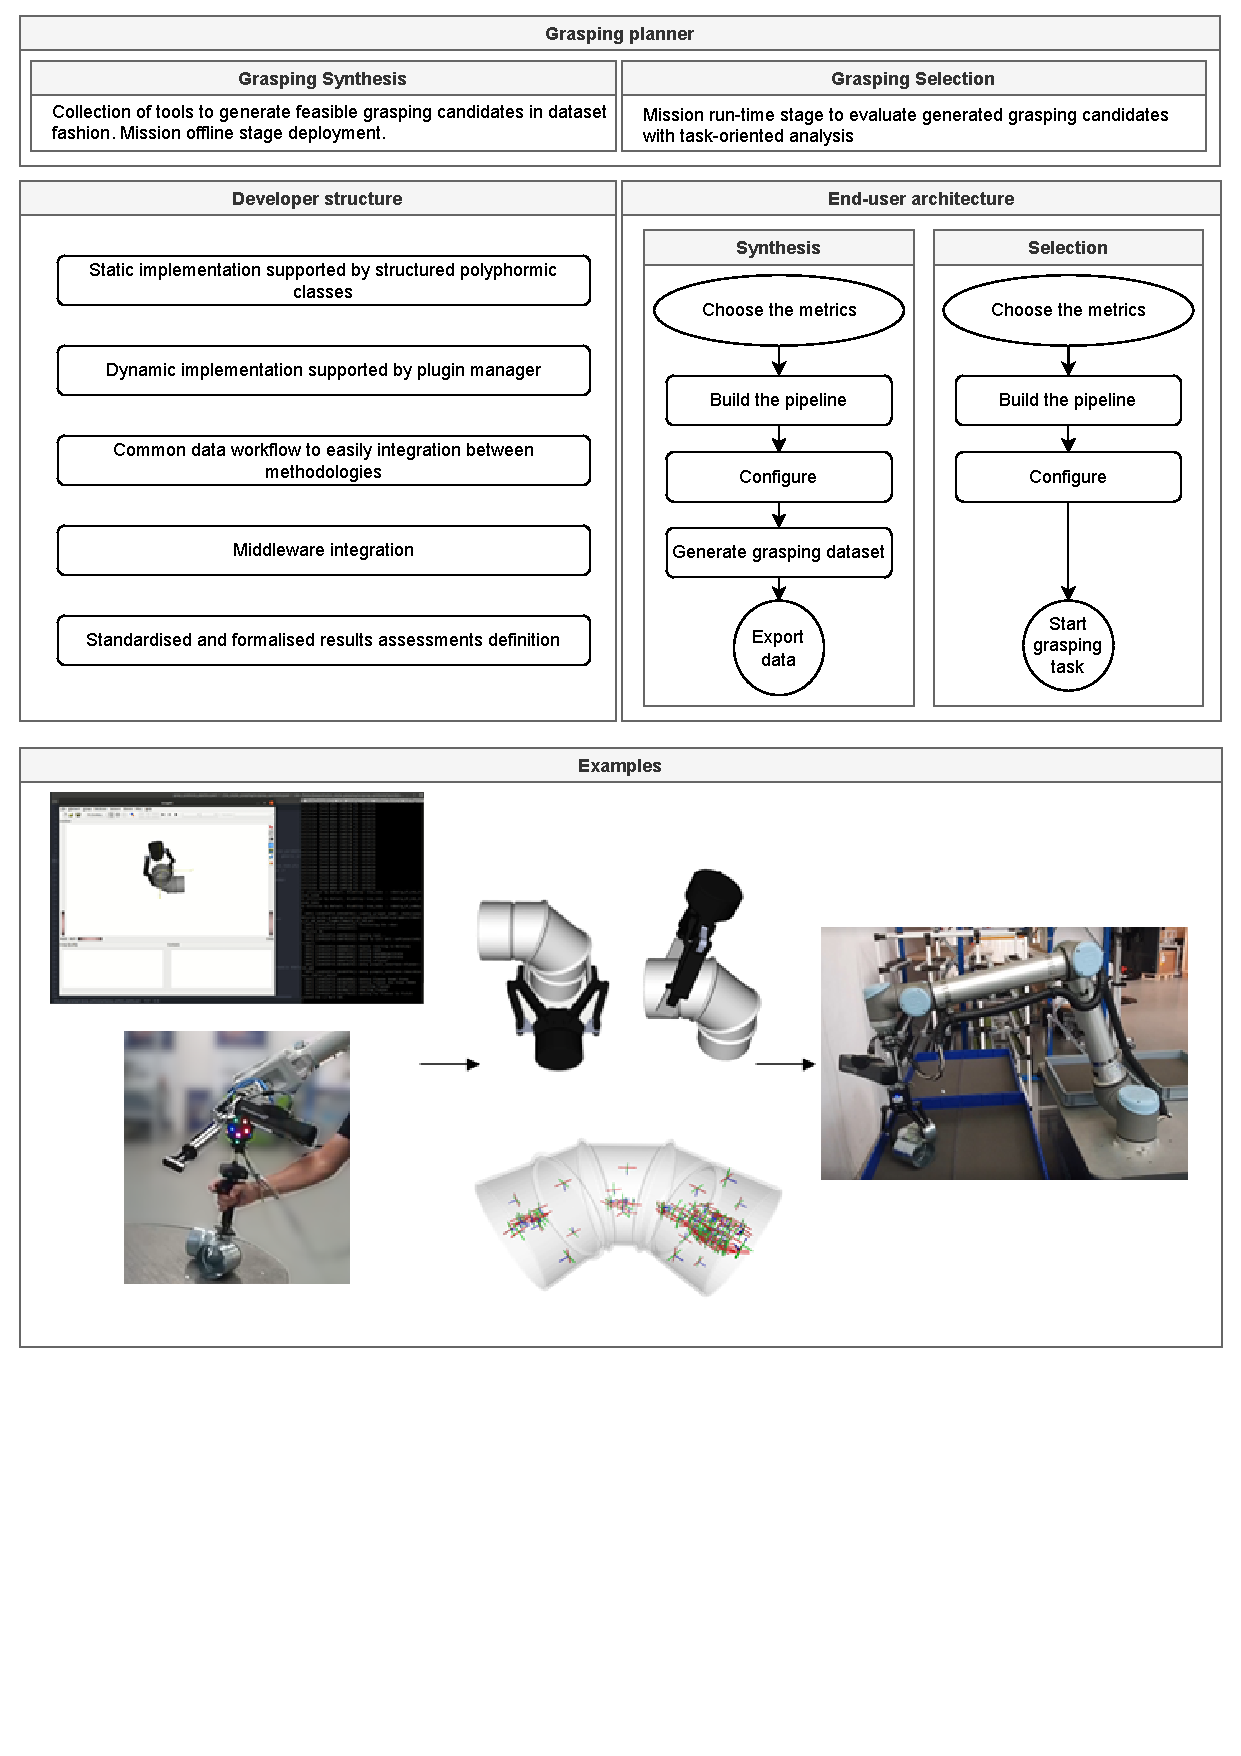
\includegraphics[trim={0cm 6.5cm 0cm 0cm},clip,width=1\linewidth,angle=0]{Cap0/Figuras/graphical_abstract_v4.pdf}}
%\caption{Graphical Abstract.}
%\label{fig:}
\end{figure}

\end{center}
%-----------------------------------------------------------------------------------------------------------------
\cleardoublepage
\phantomsection
%-----------------------------------------------------------------------------------------------------------------
\prefacesection{Agradecimentos}
%-----------------------------------------------------------------------------------------------------------------
\cred{TODO}
Meis summo ex eam, facer animal voluptaria te quo. Ad vix ancillae reprehendunt, mei integre erroribus te, eum aliquam platonem corrumpit ex. Pri tractatos definiebas ex, per alii zril diceret ea. Te per purto nulla scripta, dolorum facilis eam ea, autem dicant putent ex vis. Ad sed prima ipsum, ex cum alia simul.

In mel equidem verterem, dicta gloriatur definitionem eos ad. Mel id nulla inermis. Sed placerat reformidans at. Nibh eius eu vix, cum dolore eripuit evertitur eu, at velit phaedrum sed. At eum erant aperiri mediocrem, ius inani disputando ex. Usu aliquid moderatius disputationi te, dico ornatus moderatius an mei.

Per affert conclusionemque no. Quo et dico mazim vivendum, id senserit repudiare efficiantur vix, pri at consequat adversarium. Te quem mandamus qui, an enim laudem sed. An has omnis summo eleifend, ei sed eripuit similique.



\EspacoMedio
\EspacoMedio
\EspacoMedio
\noindent UTAD, \hfill Nome \\ Vila Real, xx de xxxxx de 20XX
%-----------------------------------------------------------------------------------------------------------------

%-----------------------------------------------------------------------------------------------------------------
\cleardoublepage
\phantomsection
\prefacesection{Publications}

This Ph.D. thesis proposal results in following publications:


%\nobibliography*

\begin{enumerate_jp}
\item \fullcite{DESOUZA2021102176}
\item \fullcite{carvalho2020}
\item \fullcite{6dmimicIMU}

\end{enumerate_jp}

%-----------------------------------------------------------------------------------------------------------------
\cleardoublepage
\phantomsection
%\prefacesection{R\&D Companion Projects and Industrial Deployment}
\prefacesection{Projects Deployment}

The following R\&D projects deployed this Ph.D. thesis proposal:

\begin{comment} %%%%%%%%%%%%%%%%%%
\begin{itemize_jp}
    \item \textbf{Fasten:} Flexible  and  Autonomous  Manufacturing  Systems  for  Custom-Designed Products. \url{http://www.fastenmanufacturing.eu/}. European Union’s Horizon 2020 research and innovation programme under grant agreement 777096.
    \item \textbf{Mari4 Yard:} Leverages the potential of Internet of Things (IoT), mobile and ubiquitous ICT tools, and robotics to develop user-centric solutions for flexible and modular manufactoring and thus implement a novel connectes shipyard. \url{https://www.mari4yard.eu/}. European Union’s Horizon 2020 research and innovation programme under Grant Agreement 101006798.
    \item \textbf{Produtech 4S\&C:} \url{http://mobilizadores.produtech.org/en/produtech-4-s-c?set_language=en}
    
    \item \textbf{Produtech SIF:} \url{http://mobilizadores.produtech.org/en/produtech-sif}
\end{itemize_jp}
\end{comment} %%%%%%%%%%%%%%%%%%



\begin{itemize_jp}
    \item \textbf{Fasten.} European Union’s Horizon 2020 research and innovation programme under grant agreement 777096. \url{http://www.fastenmanufacturing.eu/}.
    \item \textbf{Mari4 Yard.}  European Union’s Horizon 2020 research and innovation programme under Grant Agreement 101006798. \url{https://www.mari4yard.eu/}.
    \item \textbf{Produtech 4S\&C.}   European Regional Development Fund, through the Operational Programme for Competitiveness and Internationalisation - COMPETE 2020 Programme under the Portugal 2020 Partnership Agreement with reference POCI-01-0247-FEDER-046102. \url{http://mobilizadores.produtech.org/en/produtech-4-s-c}
    
    \item \textbf{Produtech SIF.} European Regional Development Fund, through the Operational Programme for Competitiveness and Internationalisation - COMPETE 2020 Programme under the Portugal 2020 Partnership Agreement with reference POCI-01-0247-FEDER-024541. \url{http://mobilizadores.produtech.org/en/produtech-sif}
\end{itemize_jp}



%-----------------------------------------------------------------------------------------------------------------
\cleardoublepage
\phantomsection
\currentpdfbookmark{\contentsname}{}
\tableofcontents%
%-----------------------------------------------------------------------------------------------------------------
\cleardoublepage
\phantomsection
\addcontentsline{toc}{chapter}{\listtablename}
%\listoftables %
%-----------------------------------------------------------------------------------------------------------------
\cleardoublepage
\phantomsection
\addcontentsline{toc}{chapter}{\listfigurename}
\listoffigures%
%-----------------------------------------------------------------------------------------------------------------
%-----------------------------------------------------------------------------------------------------------------
% Glossário de termos, lista de acrónimos e lista de abreviaturas
%-----------------------------------------------------------------------------------------------------------------
\prefacesection{Glossário, acrónimos e abreviaturas}
{
    \setlinespacing{1.33}
    \def\baselinestretch{1.15}
    \renewcommand{\arraystretch}{1.1}
    \setlength{\arrayrulewidth}{0.2mm}%
%-----------------------------------------------------------------------------------------------------------------
\section*{Glossary}
%-----------------------------------------------------------------------------------------------------------------
\vskip10mm

%-----------------------------------------------------------------------------------------------------------------
\section*{Acronym list}
%-----------------------------------------------------------------------------------------------------------------

%\begin{longtable}[c]{p{3cm} p{11cm}}
%    \textbf{Sigla} & \textbf{Expansão} \\
%    \endfirsthead
%    \textbf{Sigla} & \textbf{Expansão} \\
%    \endhead
%    \endfoot
%    \endlastfoot\\
%    SNN & \textit {Simulated Annealing} \\
%    DC & \emph{Direct Current} (corrente contínua) \\
%    
%    MOSFET & \textit {Metal-Oxide-Semiconductor Field-Effect Transistor} \\
%    
%\end{longtable}

\begin{acronym}
\acro{PbD}{Programming-by-Demonstration}
\acro{LbD}{Learning-by-Demonstration}
\acro{DL}{Deep Learning}
\acro{CNN}{Convolutional Neural Network}
\acro{FCN}{Fully Convolutional Network}
\acro{SL}{Supervised Learning}
\acro{RL}{Reinforcement Learning}
\acro{DRL}{Deep Reinforcement Learning}
\acro{MDP}{Markov Decision Process}
\acro{POMDP}{Partially Observable Markov Decision Process}
\acro{SANN}{Simulated Annealing}
\acro{SVM}{Support Vector Machine}
\acro{LbD}{Learning by Demonstration}
\acro{DLSR}{Dictionary Learning and Sparse Representations}
\acro{CGD}{Cornell Grasp Dataset}
\acro{RPN}{Region Proposal Network}
\acro{GPSR}{Grasping Prediction Success Rate}
\acro{GPT}{Grasping Prediction Time}
\acro{CPU}{Central Process Unit}
\acro{GPU}{Graphics Processing Unit}
\acro{Run-GPT}{Run-Time Grasping Prediction Time}
\acro{Offline-GPT}{Offline Grasping Prediction Time}
\acro{GPU-GPT}{GPU Grasping Prediction Time}
\acro{CPU-GPT}{CPU Grasping Prediction Time}
\acro{GRSR}{Grasping Reaching Success Rate}
\acro{GHSR}{Grasping-Holding Success Rate}
\acro{HGSR}{Handling Grasping Success Rate}
\acro{GQ-CNN}{Grasp Quality Convolution Neural Network}
\acro{IoT}{Internet of Things}
\acro{DOF}{Degree of Freedom}
\acro{ICP}{Interest Contact Point}
\acro{ICR}{Interest Contact Region}
\acro{COG}{Center of Gravity}
\acro{COBB}{Center of Bounding Box}
\acro{ROS}{Robot Operation System}
\acro{TCP}{Transmission Control Protocol}
\acro{DRL}{Dynamic Robot Localisation}
\acro{OR}{Object Recognition Package}
\acro{GUI}{Graphical User interface}


\end{acronym}

\vskip20mm
%-----------------------------------------------------------------------------------------------------------------

%-----------------------------------------------------------------------------------------------------------------



%-----------------------------------------------------------------------------------------------------------------

%-----------------------------------------------------------------------------------------------------------------
\afterpreface
%-----------------------------------------------------------------------------------------------------------------
\setlength{\parskip}{10pt}                  % Salto de par?grafo
\def\baselinestretch{1.15}
%-----------------------------------------------------------------------------------------------------------------
%-----------------------------------------------------------------------------------------------------------------
\chapter{Introduction}
\label{Ch:Introducao}
%---------------------------------------------------------------------------------------------------------------

\section{Context}

\sloppy %to force margin indentation
The robotic grasp is an important and challenging task that is still today the focus of several works. Although this function is intuitive and mastered by humans, for robots, it is a contemporary and imperative issue. The range of applications is wide, e.g., from bin-picking in the industry's logistics to a delicate and accurate human-machine interaction in domestic and collaborative robots applications.


\begin{figure}[h!]
\resizebox{1\textwidth}{!}{%
\begin{tcolorbox}
     \centering
     \begin{subfigure}[c]{0.45\textwidth}
         \centering
         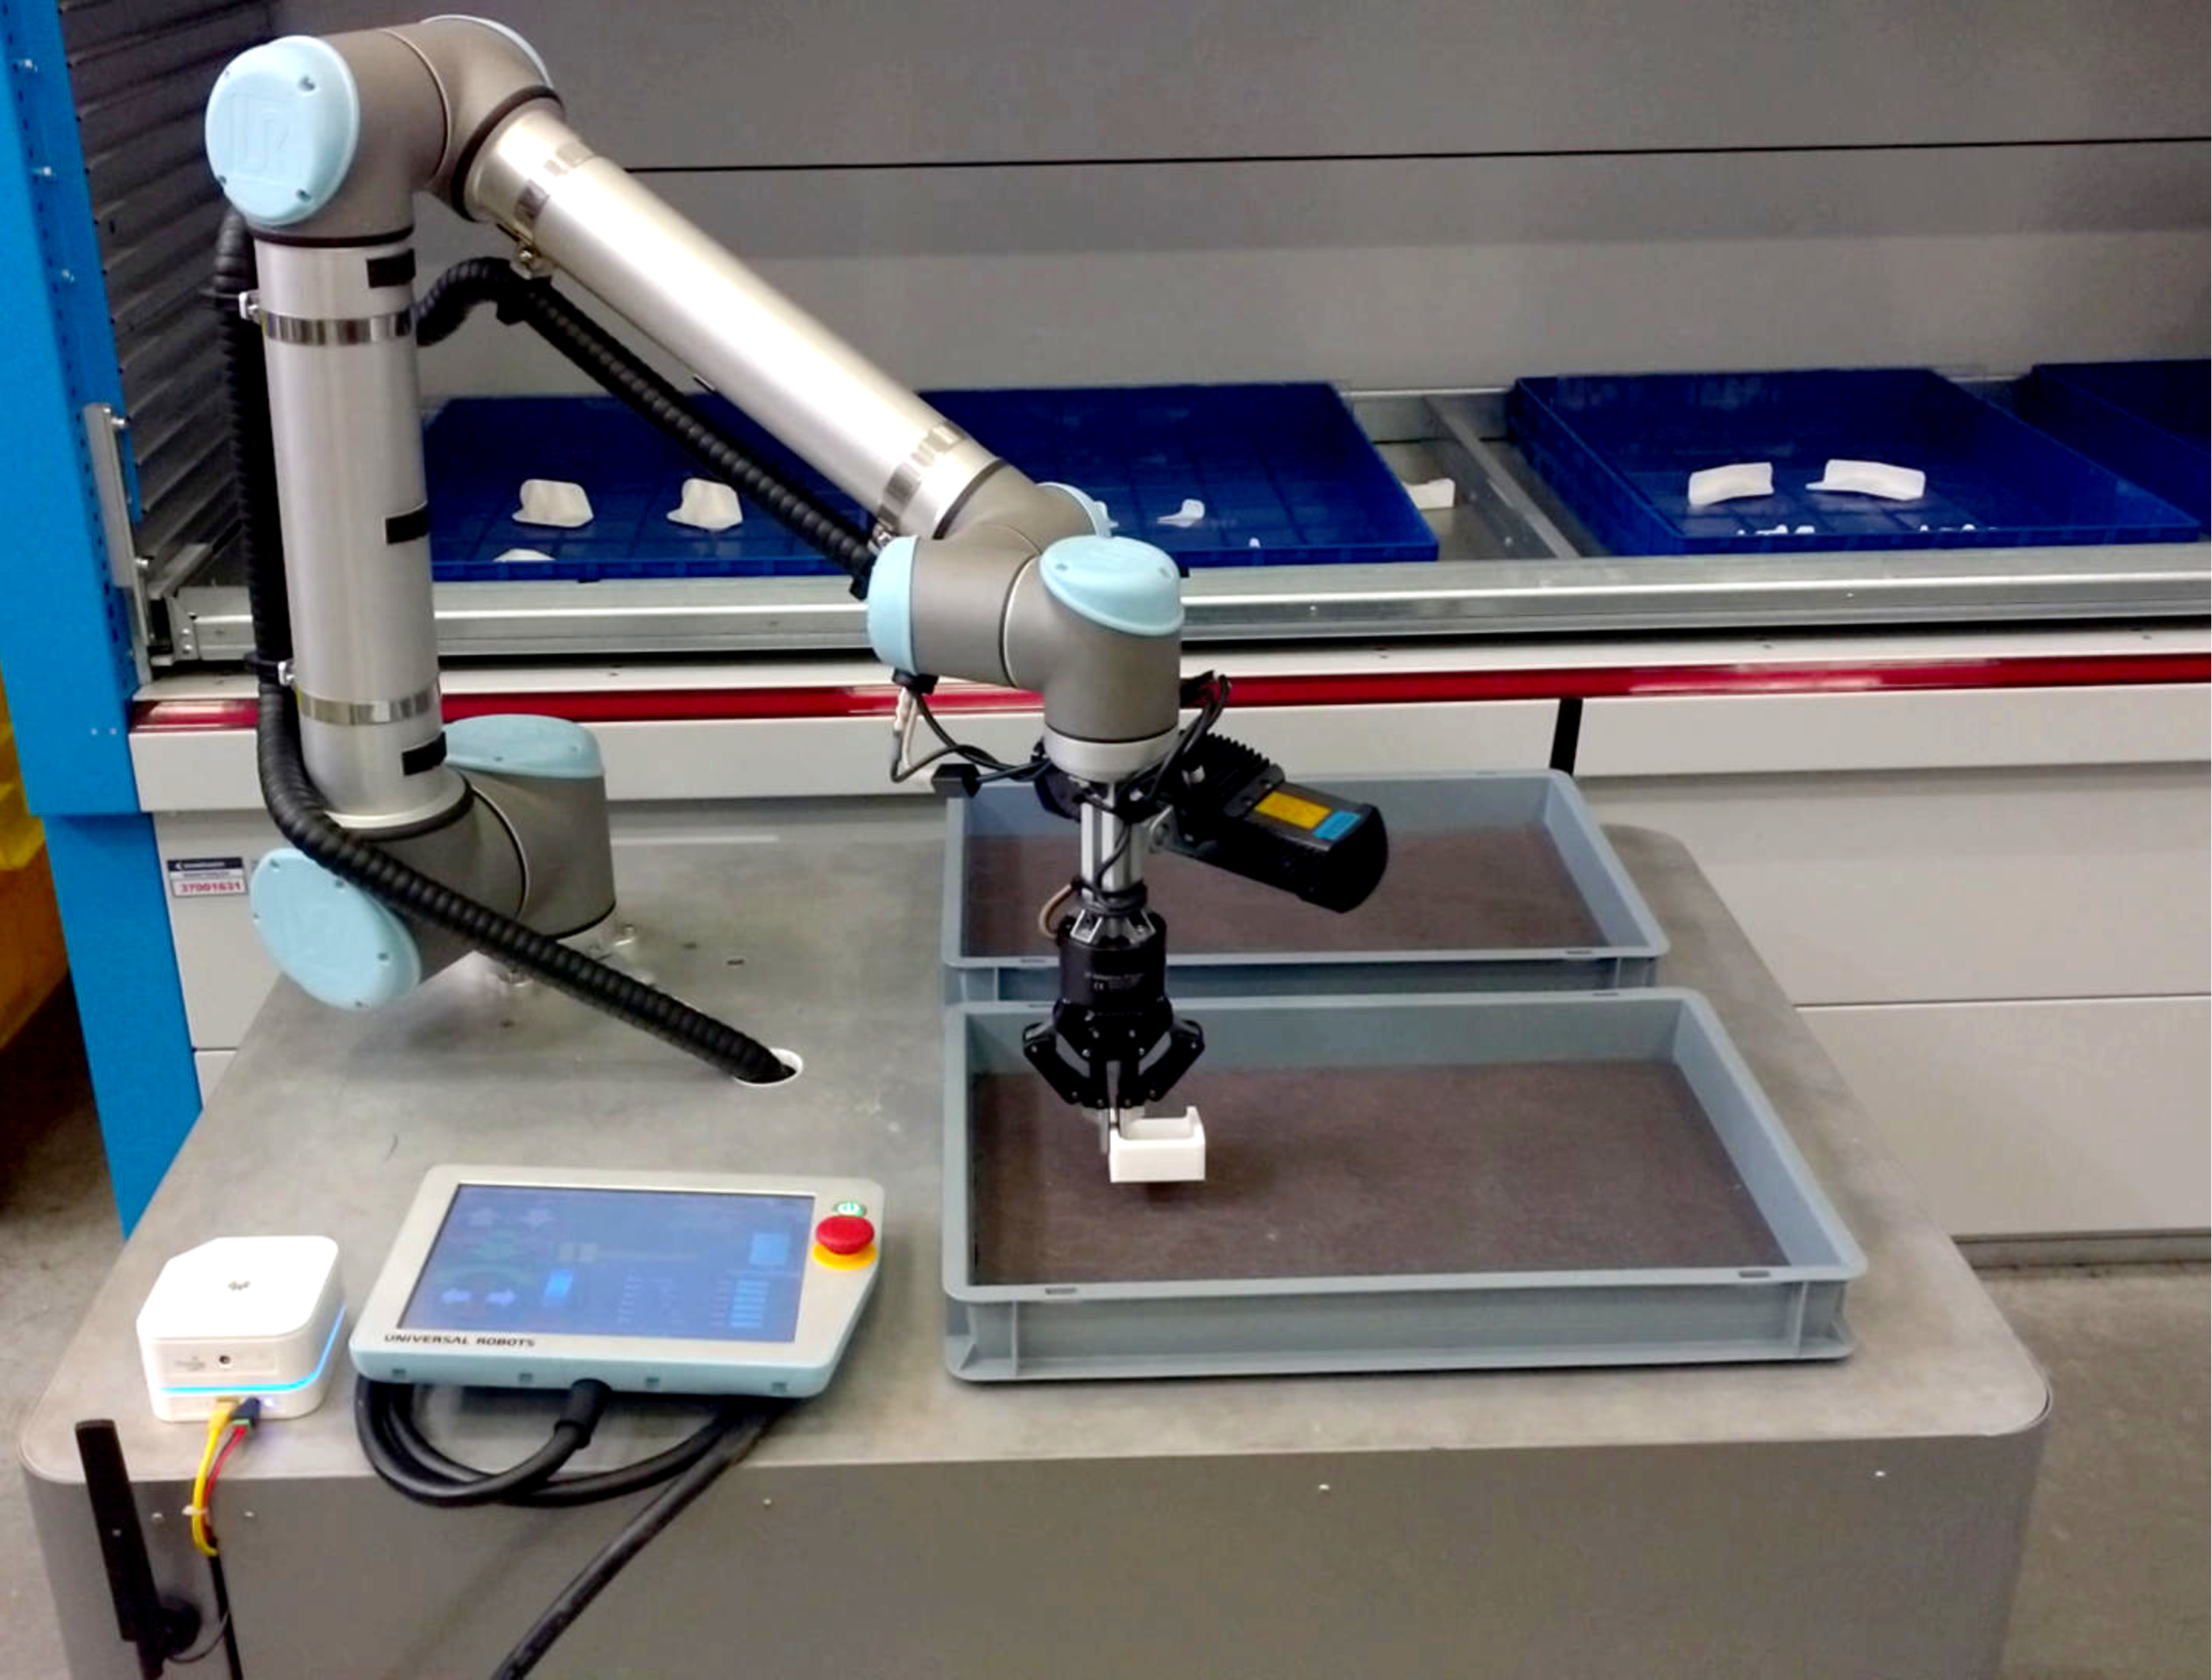
\includegraphics[width=1\textwidth]{Cap1/Figuras/platform.pdf}
         \caption{Industrial application.}
         \label{fig:g1}
     \end{subfigure}
     \hfill
     \begin{subfigure}[c]{0.45\textwidth}
         \centering
         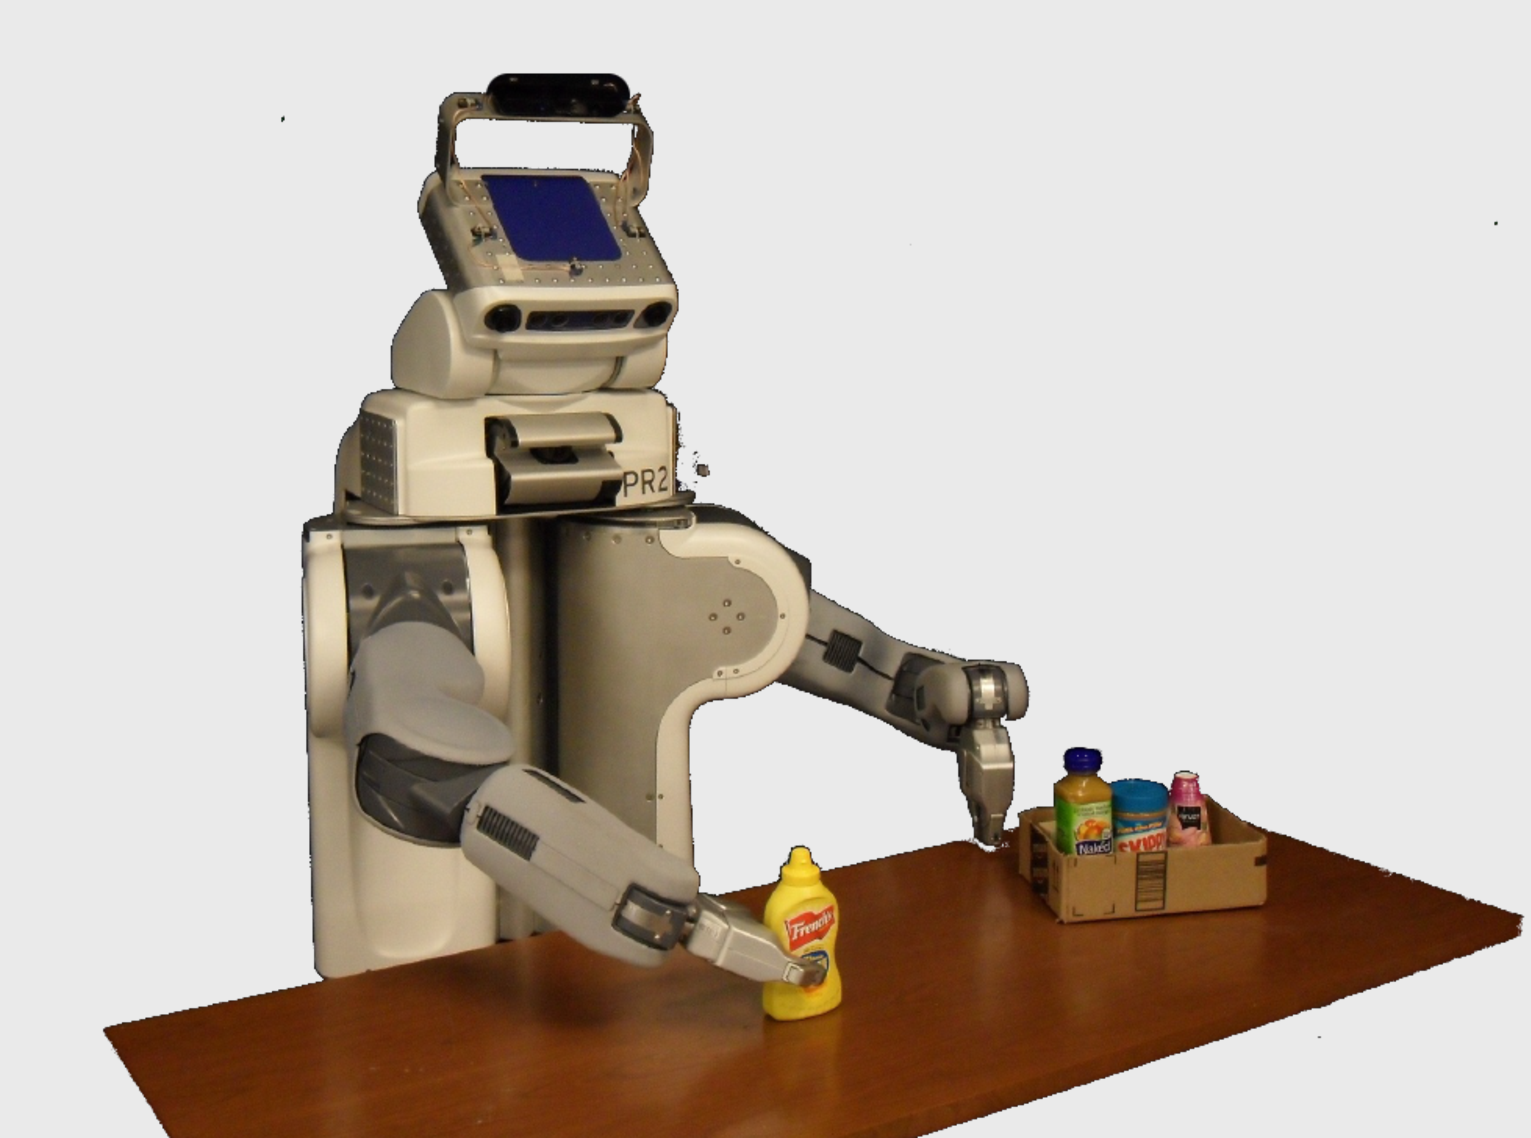
\includegraphics[width=1\textwidth]{Cap1/Figuras/pr2_grasping.pdf}
         \caption{Domestic employment~\cite{pr2robot}.}
         \label{fig:g2}
     \end{subfigure}
    \end{tcolorbox}
    \caption{Robotic grasping in different contexts.}
    \label{fig:most_usual_gripper_forms}
  }%end of resize box      
\end{figure}


In the early days, robotic manipulation was resumed as a context of human teleoperation \cite{bejczy1980sensors}. More recently, it evolved to \ac{PbD} \cite{ferreira2016stereo} and to the beginnings of \ac{LbD} \cite{suleman2011learning} even though the offline programming had been consolidated in the industrial robot programming \cite{de2020adaptpack,castro2020adaptpack}. The first studies focused on the analytical grasping modelling concerning the stability and equilibrium \cite{diziouglu1984mechanics, Nguyen1987_1, Nguyen1987_2, Ponce1995, Li2003}, besides metrics to evaluate them~\cite{Ferrari, Bicchi2000, Roa2014}. A large number of papers regarding this theme was established, achieving success grasping in specific cases. Nonetheless, the complexity rise when more general solutions are pursued: gripper's design and number of fingers~\cite{chen2020active}; previous knowledge of workpieces shape and properties \cite{babin2019stable,babin2019stable,bjornsson2018automated}, e.g., object-agnostic grasping or not; and cluttered or occluded scenes~\cite{d2020study}.

\begin{figure}[h]
\resizebox{.7\textwidth}{!}{%
\begin{tcolorbox}
\centerline{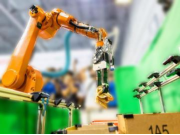
\includegraphics[trim={0cm 0cm 0cm 0cm},clip,width=1\linewidth,angle=0]{Cap1/Figuras/amazon_picking_challenge.pdf}}
\end{tcolorbox}
\caption{Amazon robotic picking challenge winner of 2017 \cite{Zeng2019}. The Amazon robotic picking challenge is an example effort to promote development the warehouse robotic grasping, such as the IROS challenge \cite{iros_challenge}}
\label{fig:}
}
\end{figure}

Subsequently, guided by computer processing and learning algorithms advancements,  works like~\cite{Saxena2008} proved that it is possible to create learning policies to grasping objects, particularly for object-agnostic grasping scenarios. Nowadays, the advent of \ac{DL} and the interesting results achieved in computer vision tasks motivate researchers to explore its capacity to grasp detection \cite{Lenz2015,Redmon2015,Kumra2017,Watson2017,Chu2018,asif2018ensemblenet, Chen2020, Guo2017,Gariepy2019,Mousavian_2019_ICCV,Ghazaei2019,TenPas2017,Chen2019,
Mahler2016,Mahler2017b, Mahler2017d, Mahler2017,Mahler2019,song2020novel}. 

Even with exciting discoveries and results successfully deployed in specific use cases, the robotic grasping still does not have a feasible generalisation solution that comprises the modern industry demands of fast design and easy deployment. It is important to note that, the results assessments standardisation is also a problem. Actually is challenging to study and choose a grasping methodology since several proposals use different results analyses that typically are not in accordance with the application necessities. 


\section{Motivation}
\label{cap1:introduction:motiviation}



%the robotic grasping still does not have a feasible generalisation solution that comprises the modern industry demands of fast design and easy deployment.

Since a complete and generic solution is unreachable until now, there is exists a lack in the deployment of a modular and flexible grasping framework for robots attending real industry demands and a well structured and formalised architecture in which organizes approaches allowing the evaluation and the base to new advancements in science. Therefore, the main Ph.D. question relies in:

\begin{flushright}
``Several approaches achieved interesting robotic grasping results in specific and/or controlled scenarios. However, how to choose and deploy them according to industry demands?"
\end{flushright}

Afterwards, when applying the grasping solution, engineers and researchers still have difficulty comparing the achieved results since the grasping parametrisation and evaluation demand big efforts. Current state-of-art deploy different metrics that, in some cases do not reflex the grasping complexity, which can involve from graspable object detection to stability estimation. Thus, the second PhD question is:

\begin{flushright}
``How evaluate a grasping methodology in a standard fashion allowing easy comparison between different techniques?"
\end{flushright}

%``Several approaches achieved interesting results in specific and/or controlled scenarios. However, how to choose and deploy them according to industry demands?"

%\cred{referenciar  ODS 9: Indústria, Inovação e Infraestruturas}

%-----------------------------------------------------------------------------------------------------------------
\section{Goals}
%-----------------------------------------------------------------------------------------------------------------

Aiming to answer the questions described in Section~\ref{cap1:introduction:motiviation}, the present thesis is summarised into two main objectives:


\begin{itemize_jp}

    \item Design of an innovative modular software architecture able to be hierarchy modified and reconfigured, structured in a pipeline flow which to organize the approaches' studies and evaluation. Therefore, developers can easily integrate new methodologies and end-users can set a pipeline of heuristics according to the task exigences and, choose between the best solution options between methodologies, i.e., the user will just need to pick the method and set its parameters without implementing the methods by self; 

    \item Formalisation and standardisation of the grasping evaluation idea since a grasping problem involves perception, planning, and control. Therefore, a clear standard could improve the methodologies' comparability since each step of the procedure affects the grasping performance. These criteria are applied in state-of-art literature and in the current work.

    %\item Discussion and presentation of the new steps and future works ideas not yet explored: from the academic field to the new challenges of industry 4.0.
    
\end{itemize_jp}

Other specific developments and contributions are highlighted as following:

\begin{itemize_jp}
    \item Discussion and review of state-of-the-art proposals regarding grasping solutions and how they evolved over the years; 
    \item Definition of a grasping dataset standard;
    \item Development of grasping hardware and firmware to support grasping by demonstration applications.
\end{itemize_jp}


%-----------------------------------------------------------------------------------------------------------------
\section{Thesis Organisation}
%-----------------------------------------------------------------------------------------------------------------


The remainder of the thesis is organised as follows: Chapter~\ref{cap2a:background} presents some theoretical background and concepts used in the present thesis. Chapter~\ref{cap2:related_work} shows and discusses the related work, from different grasping representations (since the characterisation is the most important step in any grasping planning approach) to a review of analytical, learning and deep Learning methods. Chapter~\ref{cap3:grasping_eval} presents a grasping evaluation discussion followed by the proposal of formalisation and standardisation of the grasping evaluation idea. Latter, the proposed standard is applied to state-of-art literature. The modular grasping pipeline proposal is described in Chapter~\ref{cap4:modular_grasping_architecture} with its sub-systems and hardware structures. Chapter~\ref{cap5:results} shows the proposal evaluation and test assessments. In the end, Chapter~\ref{cap6:conclusion} presents the conclusion and the future work discussion and suggestions.
 

%-----------------------------------------------------------------------------------------------------------------

%-----------------------------------------------------------------------------------------------------------------
\chapter{Technical and Theoretical Background}
\label{cap2a:background}
This chapter discusses the most important background concepts used in the current thesis. Namely, Section~\ref{sec:grippers_technolgy} is focused on explaining the existing gripper technologies and how devices and robots can grasp objects. Since a wide number of applications use multi-finger grasping, the theoretical background of this theme is presented in Section~\ref{sec:multifingered_grasping}. In the end, Section~\ref{sec:sim_ann} addresses the optimisation algorithm method embedded into the ``GraspIt!" simulator which is widely used by the academic community and further investigated in the current thesis proposal.  

%\clearpage
\section{Gripper Technologies}
\label{sec:grippers_technolgy}

End-effectors are hardware devices of handily mechanisms (e.g., robots and automation
systems) aiming them to interact with the environment.

Two classes of interaction are: passive and active.

In passive interaction, the end effectors are composed of sensors (e.g., inspection, quality assurance, and surveillance applications). Meanwhile, the active interaction consists of direct interaction with the workpiece (e.g., welding, cutting, drilling, screwing, grinding, painting, and grasping different objects).

\begin{figure}[h!]
\resizebox{0.85\textwidth}{!}{%
\begin{tcolorbox}
    \centering
    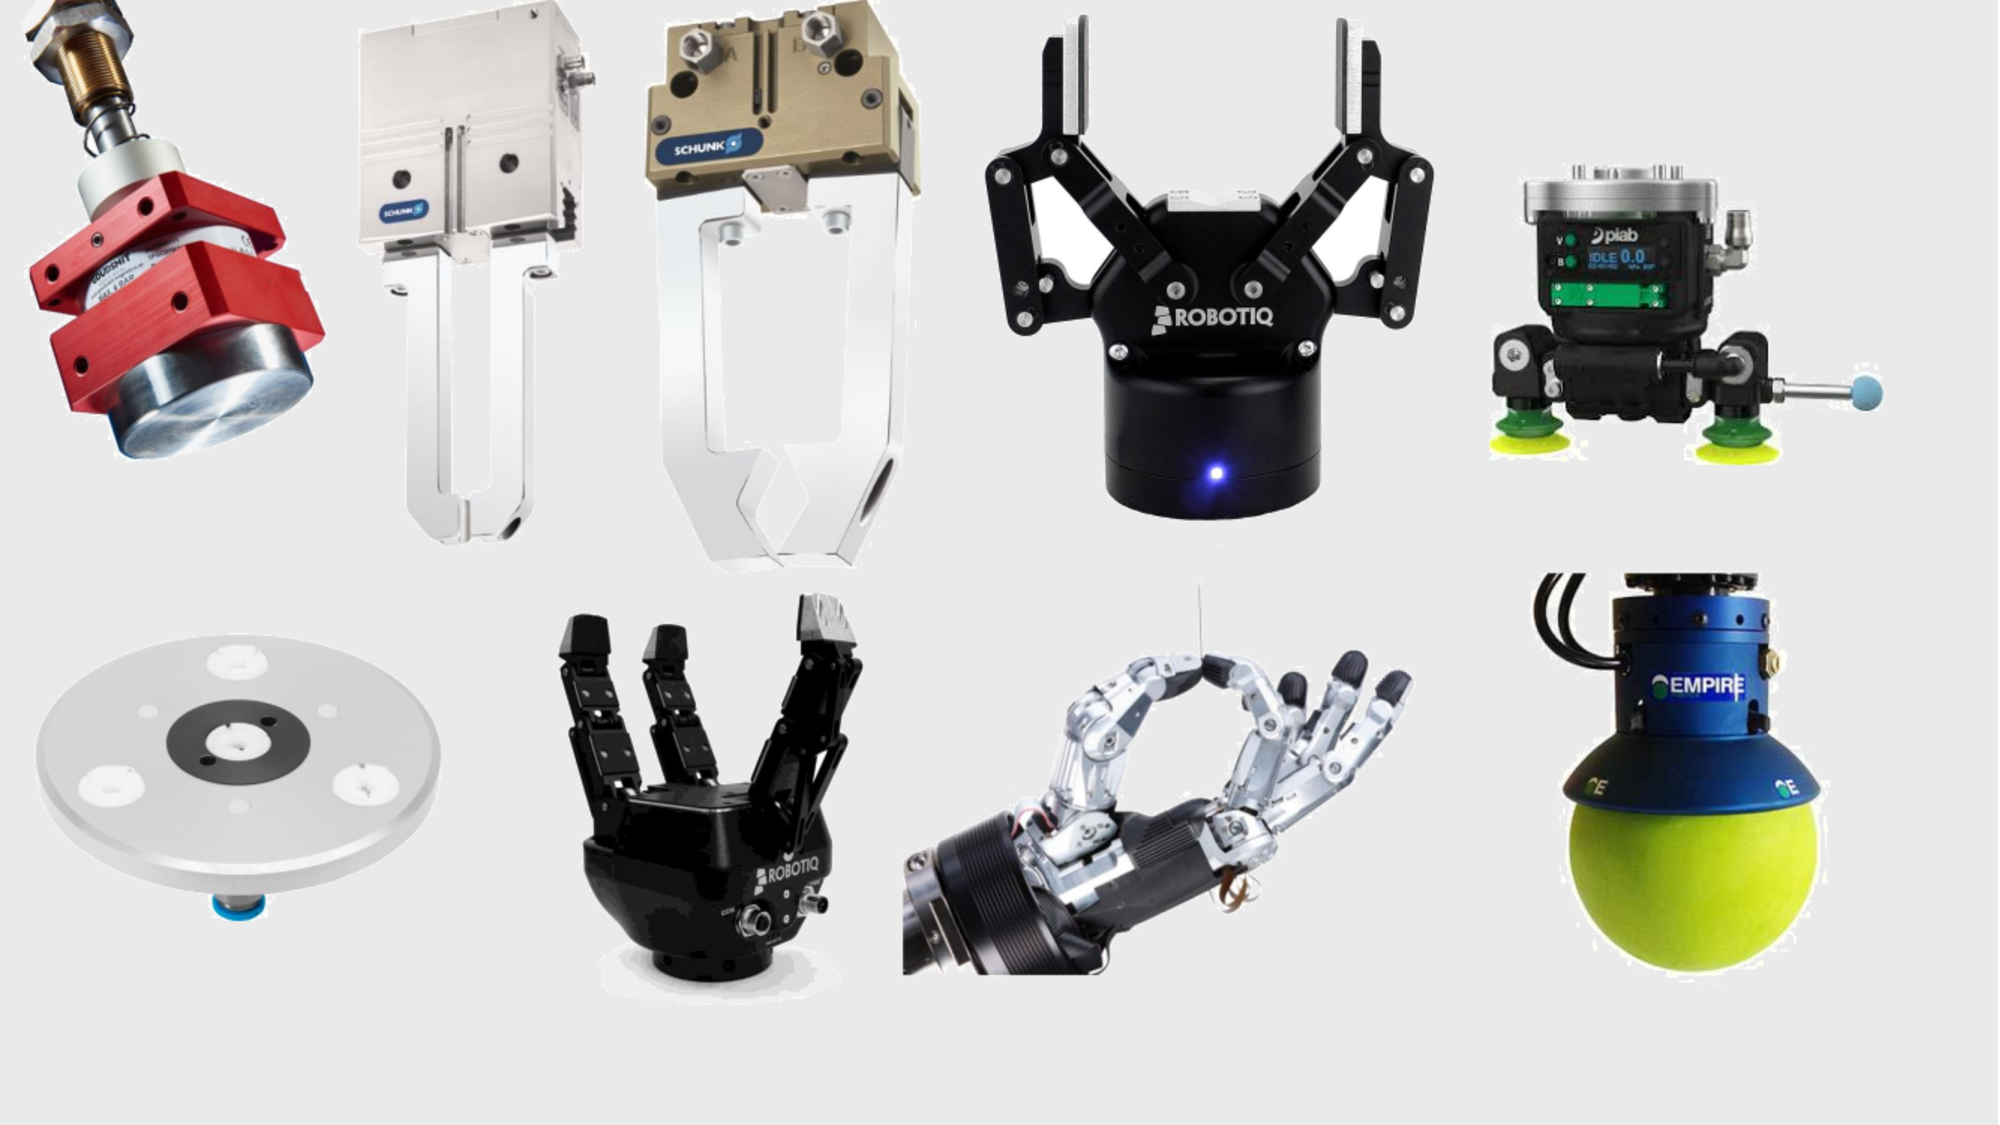
\includegraphics[trim={0mm 2cm 2cmm 0mm},clip,width=1\linewidth,angle=0]{Cap3/Figuras/grippers_list_gray_bg.pdf}
\end{tcolorbox}
    \caption{Commercial grippers examples. From top-left to down-right:  magnetic \cite{magnetic}, parallel fingers \cite{parallel}, angular fingers \cite{angular}, adaptive two-fingers \cite{robotiq_grippers}, dual suction \cite{dual_suction}, Bernoulli\cite{bernoulli}, adaptive three-fingers \cite{robotiq_grippers}, anthropomorphic \cite{anthopomorphic}, Versaball \cite{versaball}}
    \label{fig:gripper_examples}
    }%end of resize box
\end{figure}

The robotic grippers are a complex class of active end-effectors. They are active links to handle workpieces~\cite{monkman2007robot}. Grippers need to be flexible and versatile according to the application and object that they handle. Nowadays, with the development of new technologies, the variety of grippers and hardware allows more functionality, although it demands new efforts (e.g. modelling and control). In that way, hardware evaluation is also a part of the development of grasping estimation. The structure of the gripper defines a classification of grasping, related to the handling of the objects, i.e., hold an object with an emphasis in security (enveloping grasp) or dexterity and sensitivity (dexterous manipulation). The main characteristic of the dexterous is the manipulation of the object with fingers. Meanwhile, the enveloping grasping wraps the object with the palm and the finger \cite{Bicchi2000} and \cite{alonso2018current}.


Figure~\ref{fig:gripper_examples} and Figure~\ref{fig:most_usual_gripper_forms} elucidate some technologies applied in the concept of different
grippers. The most usual forms of grippers are \cite{monkman2007robot}:

\begin{itemize_jp}
    \item \textbf{Impactive}: the gripper realizes impactive forces against the surface of the workpiece. Some examples are the finger grippers.
    
    \item \textbf{Astrictive}: the gripper generates a field responsible for producing a binding force, as an air movement (vacuum suction), magnetic or electrostatic effect.
    
    \item \textbf{Contigutive}: the gripper touches a surface making contact prehension. The adhesion may be chemical or thermal effects.
    
    \item \textbf{Ingressive}: the gripper permeates the surface of the workpiece. This ingression can be intrusive (pins) or non-intrusive (e.g., hook and loop).    
\end{itemize_jp}

\begin{figure}[h!]
\resizebox{0.85\textwidth}{!}{%
\begin{tcolorbox}
     \centering
     \begin{subfigure}[c]{0.25\textwidth}
         \centering
         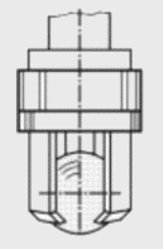
\includegraphics[width=.5\textwidth]{Apendices/Figuras/g1_gray_bg.pdf}
         \caption{Pure enclosing without clamping.}
         \label{fig:g1}
     \end{subfigure}
     \qquad
     \begin{subfigure}[c]{0.25\textwidth}
         \centering
         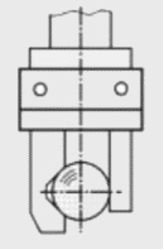
\includegraphics[width=.5\textwidth]{Apendices/Figuras/g2_gray_bg.pdf}
         \caption{Partial form fit combined with clamping force.}
         \label{fig:g2}
     \end{subfigure}
     \qquad
     \begin{subfigure}[c]{0.25\textwidth}
         \centering
         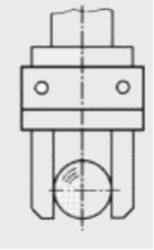
\includegraphics[width=.5\textwidth]{Apendices/Figuras/g3_gray_bg.pdf}
         \caption{Pure force closure.}
         \label{fig:g3}
     \end{subfigure}
	\qquad
     \begin{subfigure}[c]{0.25\textwidth}
         \centering
         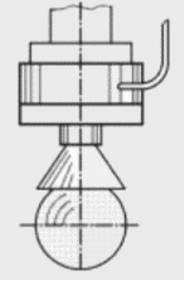
\includegraphics[width=.5\textwidth]{Apendices/Figuras/g4_gray_bg.pdf}
         \caption{Holding with vacuum air (pneumatic force closure).}
         \label{fig:g4}
     \end{subfigure}
     \qquad
     \begin{subfigure}[c]{0.25\textwidth}
         \centering
         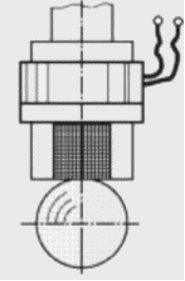
\includegraphics[width=.5\textwidth]{Apendices/Figuras/g5_gray_bg.pdf}
         \caption{Retention using magnetic field (force field).}
         \label{fig:g5}
     \end{subfigure}
     \qquad
     \begin{subfigure}[c]{0.25\textwidth}
         \centering
         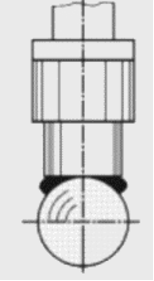
\includegraphics[width=.5\textwidth]{Apendices/Figuras/g6_gray_bg.pdf}
         \caption{Retention using adhesive media.}
         \label{fig:g6}
     \end{subfigure}
    \end{tcolorbox}
    \caption{Forms of grippers according to \cite{monkman2007robot}}
    \label{fig:most_usual_gripper_forms}
  }%end of resize box      
\end{figure}

The use of automatic tool change devices is an option to improve the flexibility, and
applicability of the grippers over the wide variety of objects and workpieces. Besides that, the use of handling machines or dual-arm robots in the automatic process is also a valid alternative (Figure~\ref{fig:alternatives}). Both solutions increase the complexity of the system, and the grasp estimation evaluation may determine which tool is best to complete the task to each object to grasp.

\begin{figure}[h!]
\resizebox{0.75\textwidth}{!}{%
\begin{tcolorbox}
    \centering
    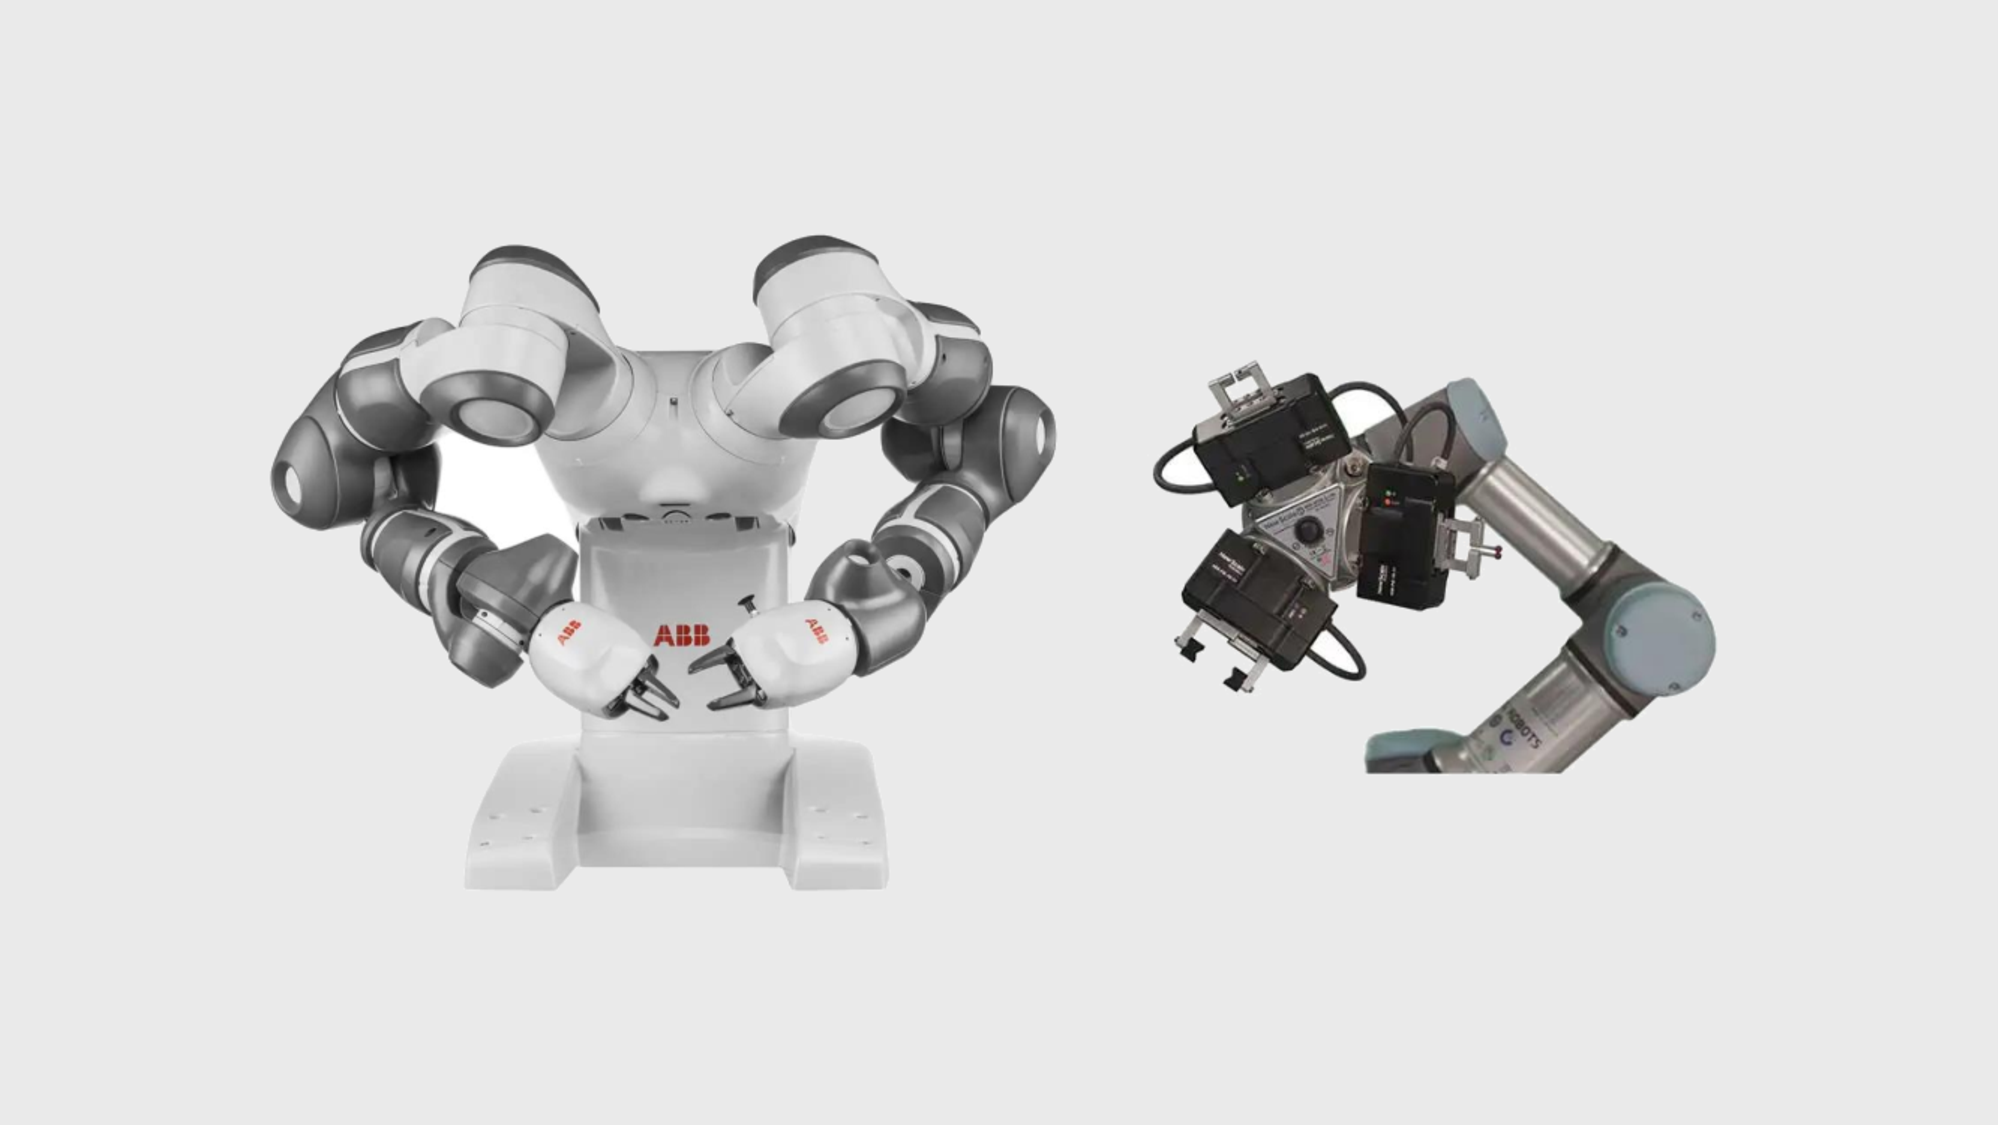
\includegraphics[trim={4cm 3cm 4cm 3cm},clip,width=1\linewidth,angle=0]{Apendices/Figuras/multi_end_effectors_gray_bg.pdf}
\end{tcolorbox}
    \caption{(left) Multi-arm robot~\cite{abb_dual_arm}. (right) Multi-gripper end-effector~\cite{multi_gripper_nsr}}
    \label{fig:alternatives}
}%end resize box
\end{figure}
%\clearpage
\section{Multi-Fingered Grasping}
\label{sec:multifingered_grasping}

A multi-fingered grasping is realised over a set of contacts between the active pairs (the workpiece and the gripper). Therefore, the determination of a suitable configuration of independent grasping points is the primary step of the fingered grasping planning. 

The wrench vectors describe the forces and moments that influence a rigid body's dynamic. These vectors can be used to formulate grasping locations, and a wrench vector is presented below:  

\begin{equation}
\mathbf{w_{c}}=\left[\begin{array}{l}
\mathbf{f} \\
\boldsymbol{\tau}
\end{array}\right]
\end{equation}

\noindent
where $\mathbf{f}$ and $\boldsymbol{\tau}$ are the vector representations of the forces and the moments. The wrench vectors have 3 and 6 \acp{DOF} in the case of $\mathbb{R}^2$ and $\mathbb{R}^3$, respectively.

The contact models can be categorised as friction-less contact, friction contact (also named hard finger contact), and soft contact~\cite{murray1994mathematical}. The focus of this chapter will be the friction contact, since this model covers the main application field of this thesis.

%The friction contact model considers the mechanical interaction between the active pairs. Therefore, the wrench convex depends on the friction contact forces, described by Coulomb model of friction: Considering the normal force $\mathbf{f_n}$, and the tangential force $\mathbf{f_t}$, static friction occurs when there is no slipping between the two surfaces of contact, that is when $\left|\mathbf{f_{t}}\right| \leq \mu_{t} |\mathbf{f_{n}}|
%$ where $\mu_{t} $ is a positive value representing the static tangential coefficient of friction. Figure~\ref{fig:friction_contact} shows an example of hard finger contact, the geometric representation of the Coulomb’s law and the friction cone convex also defined as ${FC}_{c_i}$. 

The friction contact model considers the mechanical interaction between the active pairs which is defined by Coulomb model of friction: Considering the normal force $\mathbf{f_n}$, and the tangential force $\mathbf{f_t}$, static friction occurs when there is no slipping between the two surfaces of contact, that is when $\left|\mathbf{f_{t}}\right| \leq \mu_{t} |\mathbf{f_{n}}|
$ where $\mu_{t} $ is a positive value representing the static tangential coefficient of friction. Figure~\ref{fig:friction_contact} shows an example of hard finger contact, the geometric representation of the Coulomb’s law and the friction cone convex also defined as ${FC}_{c_i}$. 

\begin{figure}[h!]
\resizebox{0.75\textwidth}{!}{%
\begin{tcolorbox}
\centerline{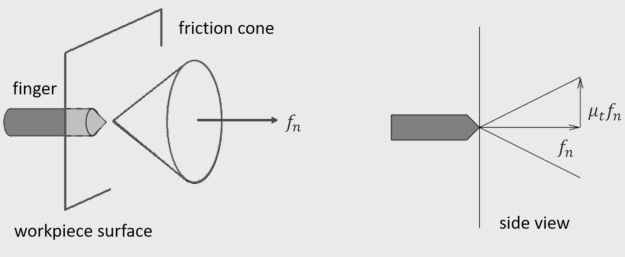
\includegraphics[trim={0cm 0cm 0cm 0cm},clip,width=1\linewidth,angle=0]{Apendices/Figuras/friction_contact_gray_bg2.pdf}}
\end{tcolorbox}
\caption{Friction contact model and the geometric representation of Coulomb’s law (figure based on~\cite{murray1994mathematical}).}
\label{fig:friction_contact}
} %end resize box
\end{figure}

A wrench representation, w.r.t the $i$-th contact point ($c_i$), could be defined as follows:

\begin{equation}
\mathbf{W_{c_i}}=\begin{bmatrix}
1 & 0 & 0 \\ 
0 & 1 & 0 \\ 
0 & 0 & 1 \\ 
0 & 0 & 0 \\ 
0 & 0 & 0 \\ 
0 & 0 & 0 
\end{bmatrix} \mathbf{f}_{c_i}, \quad \mathbf{f}_{c_i} \in F C_{c_i}
\end{equation}

\noindent
where $F C_{c_i}=\mathbf{f} \in \!R^3: \sqrt{f_{x}^{2}+f_{y}^{2}} \leq \mu_{t} f_{z,}, f_{z} \geq 0$, and $\mu_t$ is the transversal friction coefficient in $c_i$. 

Therefore, based on this wrench representation, it is possible to define the matrix that compose the wrench vector concept:

\begin{equation}
\mathbf{W}_{c_i}=\mathbf{B}_{c_i} \mathbf{f}_{c_i}, \quad \mathbf{f}_{c_i} \in F C_{c_i}
\end{equation}

\noindent
where $\mathbf{{B}_{c_i}}$ is the wrench basis matrix with dimension $p \times n$ where $p$ is the \acp{DOF} and $n$ the number of independent forces and moments that constitutes $\mathbf{{f}_{c_i}}$. The contact model discussed here has as reference frame the one with the origin coincident with the contact point itself. It is more convenient to refer all contacts in a grasp model to a common frame, generally the centre of mass of the work piece. Therefore the wrench transformation matrix is defined as follows:

\begin{equation}
^{o} \mathbf{Tw}_{c_i}=\left[\begin{array}{cc}
{^{o} \mathbf{R}_{\mathrm{c_i}}} & {0} \\
{^o \hat{\mathbf{t}}_{\mathrm{c_i}} {}^{o} \mathbf{R}_{\mathrm{c_i}}} & {^{o} \mathbf{R}_{\mathrm{c_i}}}
\end{array}\right]
\in \mathbb{R}^3
\end{equation}

\noindent
where $ ^o\mathbf{R}_{c_i}$ and $^o\mathbf{t}_{c_i}$ are the rotation and translation matrix of the $i$-th contact point ($c_i$) w.r.t. object frame ($o$). The $\mathbf{\hat{t}}$ is the linear operator representing the cross product $^o\mathbf{t}_{c_i} \times {{{}^o}\mathbf{R}}_{c_i}$ as bellow:

\begin{equation}
\widehat{\boldsymbol{a}}=\left[\begin{array}{ccc}
0 & -a_{3} & a_{2} \\
a_{3} & 0 & -a_{1} \\
-a_{2} & a_{1} & 0
\end{array}\right] \quad where \quad \boldsymbol{a} = \left[\begin{array}{c}
a_{1} \\
a_{2} \\
a_{3}
\end{array}\right]
\end{equation}


Hence, the contact map $\mathbf{G}_{i}$ is defined as follows:

\begin{equation}
\mathbf{G}_{i}=^{o} \mathbf{T} \mathbf{w}_{c_i}^{\prime} \mathbf{B}_{c_i}
\end{equation}

Note that it describes the direction of each component of the $i$-th applied wrench and defines the constraints of the contact. The grasp map is the matrix with all contact maps that characterise the contact model (it is also named constraint matrix):

\begin{equation}
\mathbf{G}=\left[\begin{array}{llll}
{{}^o \mathbf{T} \mathbf{w}_{c_1}^{\prime} \mathbf{B}_{c_1}} & {\dots} & {{}^{o} \mathbf{T} \mathbf{w}_{c_N}^{\prime} \mathbf{B}_{c_N}}
\end{array}\right]
\end{equation}

Then, including the magnitude of the forces, a workpiece wrench can be written:

\begin{equation}
^{o} \mathbf{W}=\left[\mathbf{G}_{1}, \ldots, \mathbf{G}_{N}\right]\left[\mathbf{f}_{c_1}, \ldots, \mathbf{f}_{c_N}\right]^{\prime}=\mathbf{G} \mathbf{F}
\end{equation}

\noindent
where: $\mathbf{F} \in F C \text { and } F C=F C_{c_1} \times \ldots \times F C_{C_N}$

The grasp map is an important matrix since it is the mathematical formulation of a multi-finger grasping. From now on, the common reference frame is defined as the object frame, and for convenience, the $^{o}\mathbf{W}$ will be substituted by $\mathbf{W}$. Each column of $\mathbf{W}$ represents the independent contact wrenches. All the contacts discussed here are punctual contacts since the other kinds of contact can be approximate by a set of punctual contacts and edge contacts.

By means of the convex linearisation of the friction contact, Figure~\ref{fig:friction_contact_linearised}, it is possible to represent the contact force ($\mathbf{f}_{c_i}$) as a linear combination of the cone edges ($\mathbf{S}_{c_i}$) and ($a_d$):

\begin{figure}[h!]
	\resizebox{0.75\textwidth}{!}{%
		\begin{tcolorbox}
			\centerline{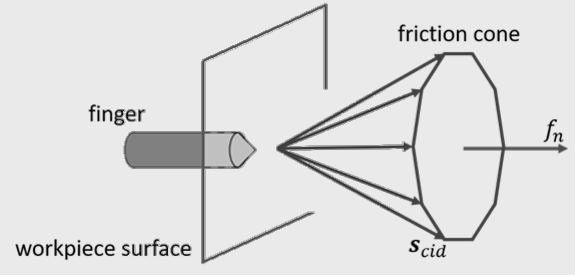
\includegraphics[trim={0cm 0cm 0cm 0cm},clip,width=1\linewidth,angle=0]{Apendices/Figuras/friction_contact_linearised.pdf}}
		\end{tcolorbox}
		\caption{Linearised friction contact model.}
		\label{fig:friction_contact_linearised}
	} %end resize box
\end{figure}


\begin{equation}
	\mathbf{f}_{ci} \approx \sum_{d=0}^{D} a_{d} \mathbf{s}_{ci_d}, a_{d} \geq 0 \quad, \quad \sum_{d=0}^{D} a_{d}=1
\end{equation}

where D is the number of edges that composes the linearised cone. A matrix notation can be formed as:

\begin{equation}
	\mathbf{f}_{ci}=\mathbf{A} \mathbf{S}_{ci}^{\prime}
\end{equation}

with $\mathbf{A}=\left[a_{0}, \ldots, a_{D}\right]$ and $\mathbf{S}_{ci}=\left[\mathbf{s}_{ci_0}, \ldots, \mathbf{s}_{ci_D}\right]$

Therefore, including all contact forces, the $\mathbf{W}$ associate with $\mathbf{S}$ is called primitive grasp map, also referred as primitive wrench map, defined as follow:

\begin{equation}
	\mathbf{W}_{p}=\left[\mathbf{G}_{1}, \ldots, \mathbf{G}_{N}\right]\left[\mathbf{A} \mathbf{S}_{c 1}^{\prime}, \ldots, \mathbf{A} \mathbf{S}_{c N}^{\prime}\right]^{\prime}=\mathbf{G} \mathbf{F}_{\mathbf{p}}
\end{equation}

The columns of $\mathbf{W}_{p}$ represent all wrenches associated with the edges of the linearised friction cone of the N contacts. It is an interesting matrix since it defines boundary conditions of contact. Applying a torque factor $\alpha$ (ensuring $|\tau| \leq|F|$) in each $w_{pd_{ci}}$ in $\mathbf{W}_{p}$, i.e.:

\begin{equation}
	w_{c}=\left[\begin{array}{c}
		\boldsymbol{f} \\
		\alpha \boldsymbol{\tau}
	\end{array}\right]
\end{equation}

and defining $\alpha=\frac{1}{r}$, where $r$ is the maximum radius of the centre of mass or gravity of the object and a contact point, it is possible to evaluate the grasps independently of the object size.

The $\mathbf{W}_p$ of all contact forces also defines the GWS (grasp wrench space) of the grasping. It is obtained by means of the $L_\infty$ or $L_1$ norm over the vector $\mathbf{g}$ composed by the magnitude of each contact normal force. The $L_\infty$ defines the GWS($W_L\infty$) considering the limitation of the maximum allowable normal contact force, while $L_1$ defines the GWS($W_{L1}$) by the sum magnitude of the normal contact forces. The norms operation yields to:


\begin{equation}
\begin{aligned}
\mathbf{W}_{L_{1}} &=\text { ConvexHull }\left(\bigcup_{c_i}^{N} \mathbf{w}_{p_1 c_i}, \ldots, \mathbf{w}_{p D_{c_i}}\right) \\
\mathbf{W}_{L_{\infty}} &=\text { ConvexHull }\left(\bigoplus_{c i}\left\{\mathbf{w}_{p_1 c_i}, \ldots, \mathbf{w}_{p D_{c_i}}\right\}\right)
\end{aligned}
\end{equation}

\noindent
where $\mathbf{w}_{pd_{ci}}$ $\in$ $\mathbf{W}$ and $\bigoplus$ is the Minkowski sum. More detail about the norm operation can be verified in~\cite{Ferrari}.


The concept of grasp closure evaluates the restraining of an object. A common assumption is the force-closure implies an equilibrium, but the inverse does not apply. A grasp has its convex hull defined by the wrenches that constitute the grasp configuration, i.e., the matrix $\mathbf{W}$. In a force-closure grasp, the convex hull includes the wrench space origin $\{O\}$, see Figure~\ref{fig:gws_force_closure}. According to the definition presented in~\cite{salisbury1983kinematic}, if all wrenches in $\mathbf{W}$ positively span the entire wrench space, the grasp will be force-closure. Figure~\ref{fig:gws_force_closure} shows a  grasp wrench space (GWS) and a convex hull of grasp configuration for force and non-force-closure, for a planar case with a fixed value for the moment ($\tau$) in the z-axis. Therefore, it is considered $\mathbf{f}_{c_i} \in  \mathbb{R}^2:  {f}_{c_i}  = (f_{x} , f_{y})$, and  the resistance to perturbation in both force axes is evaluated. 

\begin{figure}[h!]
\resizebox{0.8\textwidth}{!}{%
\begin{tcolorbox}
\centerline{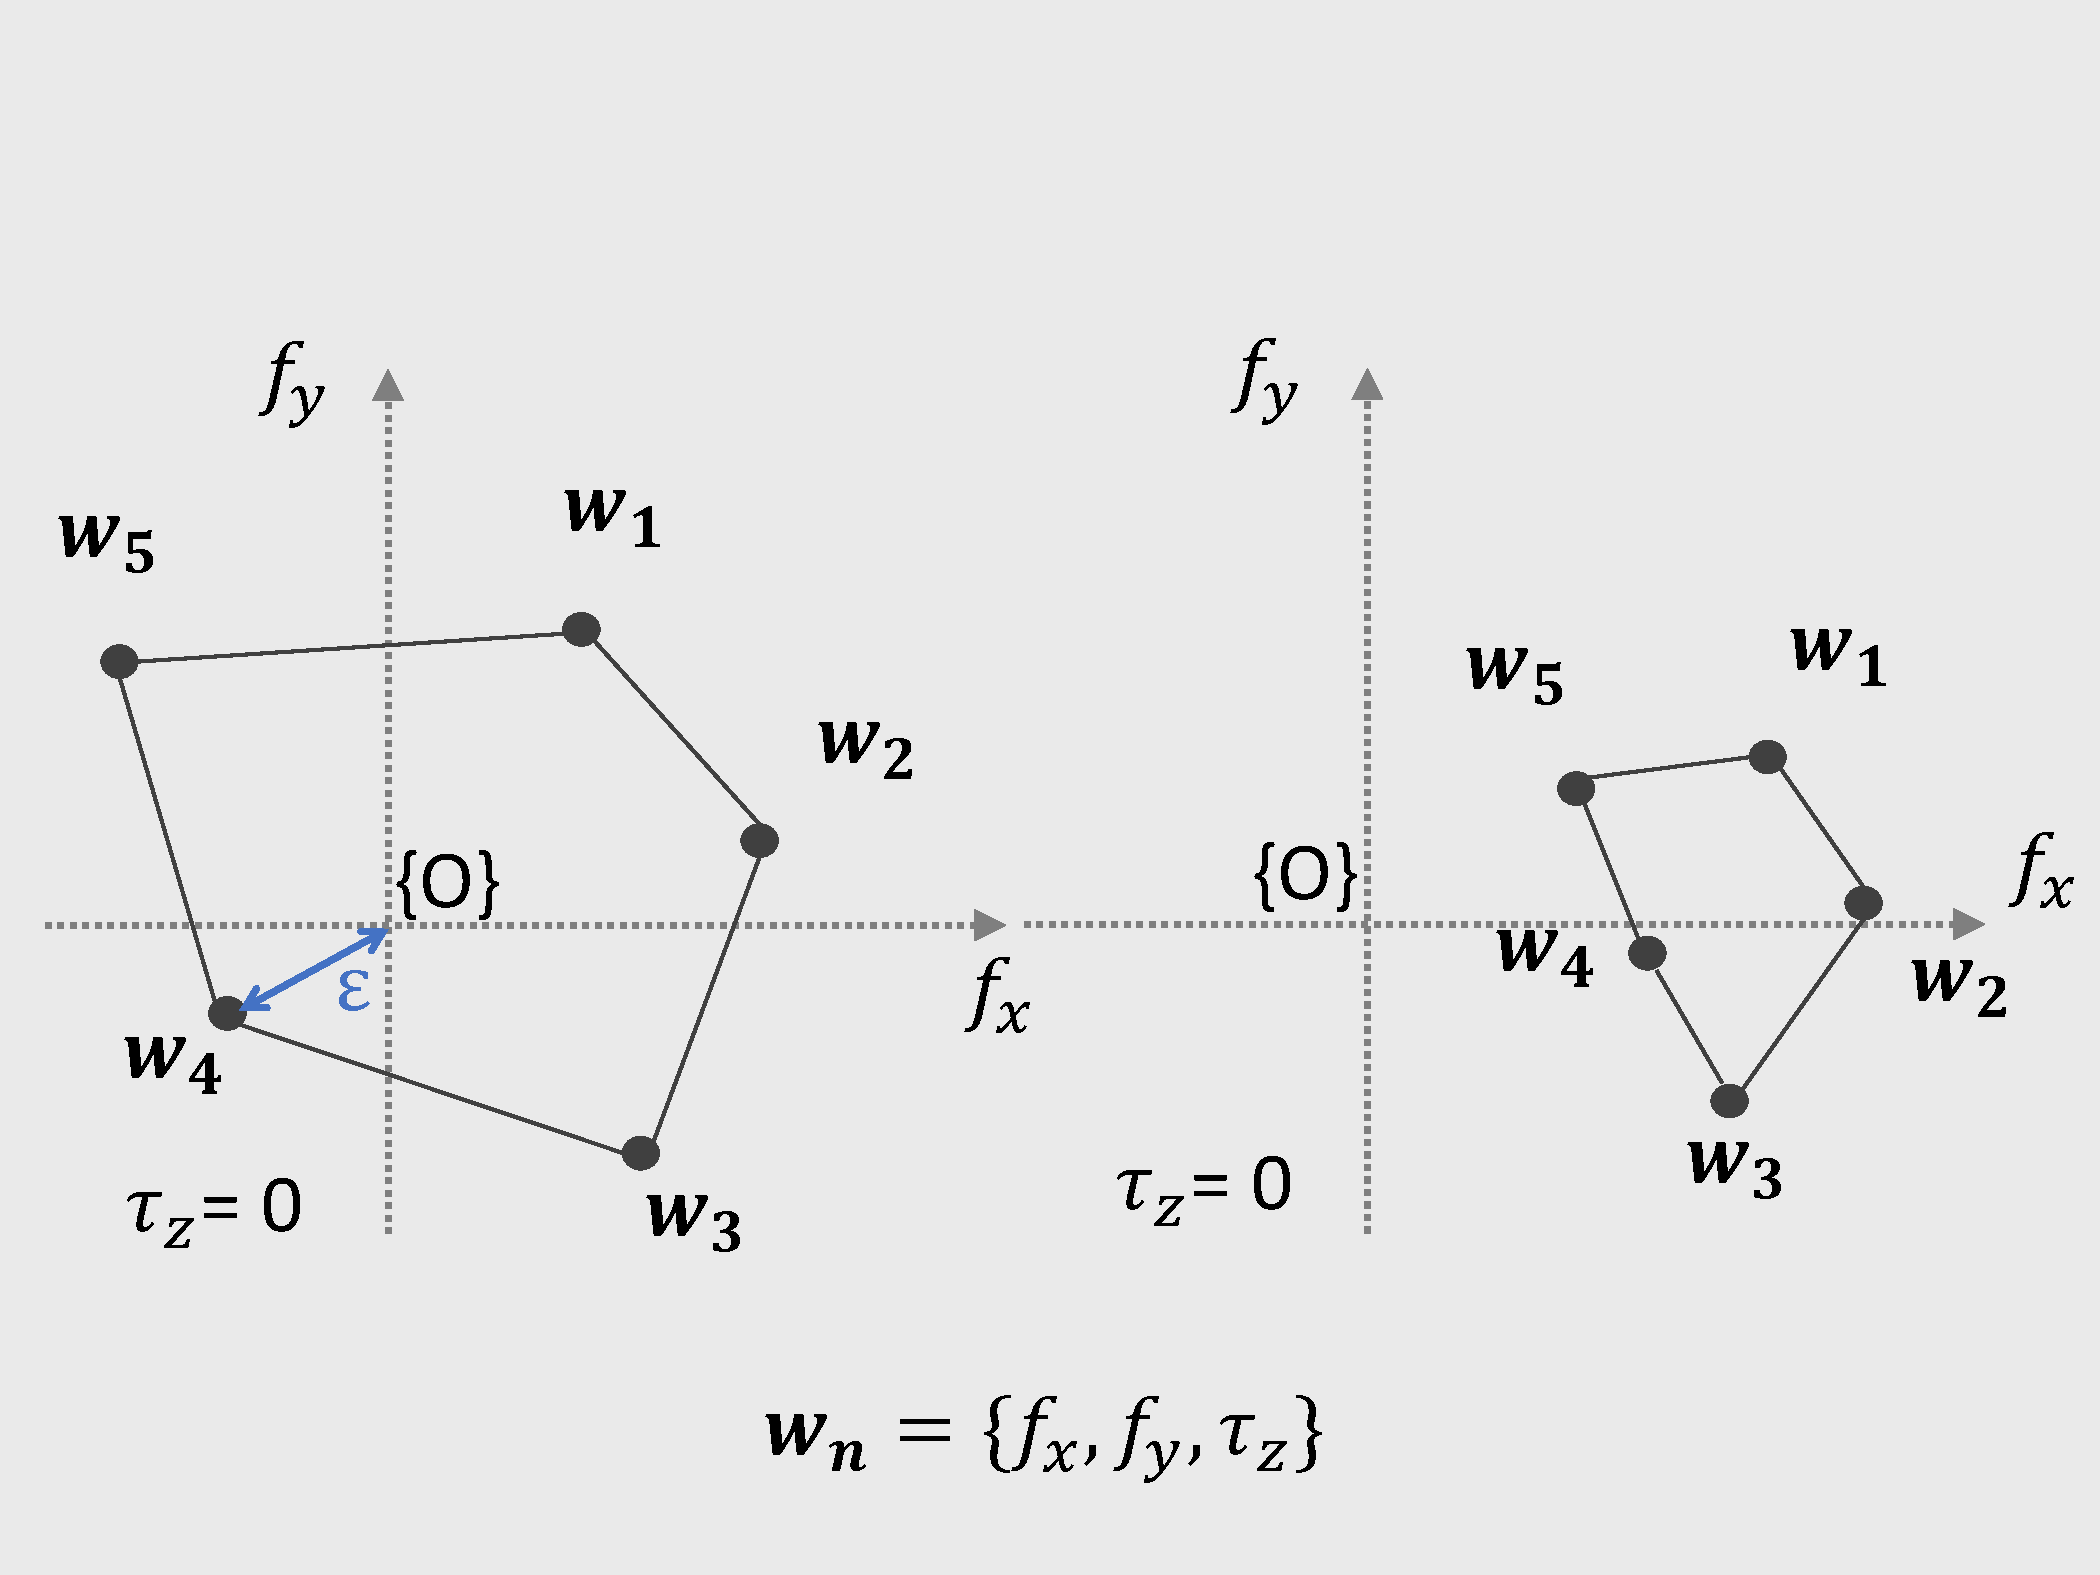
\includegraphics[trim={0cm 1.2cm 0cm 5.5cm},clip,width=1\linewidth,angle=0]{Cap2/Figuras/wrenchspace_anlayses_2.pdf}}
\end{tcolorbox}
\caption{Wrench convex-hull configuration. Force-closure and the $\epsilon$-value (left). Non-force-closure (right).}
\label{fig:gws_force_closure}
}%end resize box
\end{figure}

Since several configurations can reach a force-closure grasp, quality metrics like $\epsilon$-metric evaluate which one is best. The $\epsilon$ is a normalized value that represents the wrench vector's distance to the origin ($\{O\}$), which is the shortest, i.e., the worst wrench vector to support an external perturbation. An efficient grasp, ideally, has $\epsilon=1$ . The left GWS of Figure~\ref{fig:gws_force_closure} elucidates this metric and the readers are encouraged to a more detailed review of this grasping definition in~\cite{Ferrari}.



%\clearpage
\section{Simulated Annealing Grasping}
\label{sec:sim_ann}

The \ac{SANN} algorithm~\cite{Ciocarlie2009} integrated in the ``GraspIt!'' simulator~\cite{AndrewT2004} is one of the tools that the grasping pipeline relies on. Since it was used from the perspective of an end user, a brief explanation will be done here, and any further information can be retrieved on the referenced papers.

The \ac{SANN} is a heuristic optimization algorithm based on the cooling of a set of atoms to a minimum state of energy, and it was first introduced by~\cite{kirkpatrick1983} in a Statistical Mechanics optimization algorithm application. The ``Very Fast Simulated Re-Annealing'' was an improvement made by Ingber at~\cite{ingber1988} and used here. Since it is based on temperature, Ingber proposed that its cooling process decrease as described by Equation~\ref{eq:temperature}

\begin{equation}
T=T_{0} \cdot exp{(-k^{1/D})}
\label{eq:temperature}
\end{equation}

\noindent
where $D$ is the dimensional search space, $k$ a \ac{SANN} parameter step, and $T_0$ is the initial temperature.

Each algorithm iteration generates new state variables following a rule of neighbouring. Considering current and a new variable state as $S_{current}$ and $S_{new}$, this rule yields Equation~\ref{eq:neighbors}.

\begin{equation}
S_{new}=S_{current}+T \cdot(-1)^{round(Rand(0,1))} \cdot\left(1+\frac{1}{T}\right)^{Rand(-1,1)}
\label{eq:neighbors}
\end{equation}

\noindent
and the probability to change the state between the current and the new one is defined by Equation~\ref{eq:very_fast_snn_prob} where $Q(\bullet)$ represents the objective function of the optimization problem.

\begin{equation}
exp({\frac{Q(S_{current})-Q(S_{new})}{T}})>Rand(0,1)
\label{eq:very_fast_snn_prob}
\end{equation}

Regarding the multi-fingered grasping, it is possible to define a state based on the hand posture $\mathbf{p}$ and, the position and orientation of the wrist $\mathbf{w}$ such as:

%\begin{equation}
%S=[\mathbf{p}, \mathbf{w}], \quad \mathbf{p} \in \mathcal{R}^{d}, \mathbf{w} \in \mathcal{R}^{6}
%\label{eq:fob_grasp}
%\end{equation}

\begin{equation}
	\mathbf{S}=\left[\begin{array}{c}
		\mathbf{p} \\
		\mathbf{w}\end{array}\right], \quad \mathbf{p} \in \mathcal{R}^{d}, \mathbf{w} \in \mathcal{R}^{6}
\label{eq:fob_grasp}
\end{equation}

\noindent
where $d$ is the number of intrinsic \acp{DOF} of the hand. For instance, the human hand and the robotic Barrett gripper~\cite{barret_hand} have 20 \acp{DOF} and 4 \acp{DOF}, respectively.

As discussed by~\cite{Ciocarlie2009}, the hand posture is defined by \textit{eigengrasps}, a subspace of movement based on how human generate hand postures. The \textit{eigengrasps} reduces the \acp{DOF} of the hand based on how humans select appropriate grasps and hand postures in a primitive fashion. Studies show that humans simplify, unconsciously, the problem with a pattern in the movement. More information can be verified in~\cite{Ciocarlie2009,Santello2002}. 

Considering a hand with $d$ hand's postures DOFs, it is possible to defined a d-dimensional \textit{eigengrasp} ($\mathbf{e}_i$) as:

\begin{equation}
	\mathbf{e}_{i}=\left[\begin{array}{llll}
		e_{i, 1} & e_{i, 2} & \ldots & e_{i, d}
	\end{array}\right]
\end{equation}

\noindent where each $e_{i,d}$ represents the individual joint direction movement. In other words, the \textit{eigengrasp} ($\mathbf{e}_i$) is a d-dimensional direction vector that represents the motion of a group joint space. Therefore, it is possible to create a set of \textit{eigengrasps} with size $b \ll  d$, simplifying the searching space. Hence, a posture can be defined by Equation~\ref{eq:eigengrasp_posture}.

\begin{equation}
p=\mathbf{p}_m+\sum_{i=1}^{b} a_{i} \mathbf{e}_i
\label{eq:eigengrasp_posture}
\end{equation}


\noindent
with posture origin defined by $\mathbf{p}_m$ and $b$ the total number of \textit{eigengrasps}. Since it is a linear combination, the parameter array $\mathbf{a} = [a_1, a_2, ... , a_b]$  will be the optimisation variable in Equation~\ref{eq:fob_grasp} together with the $\mathbf{w}$. Therefore, the dimensional search space $D$ has a reduced length, i.e. $D = sizeof(\mathbf{a}) +  sizeof(\mathbf{w})$. The Figure~\ref{fig:barrett_eigengrasps} elucidates the \textit{eigengrasp} discussion in the case of 4 \ac{DOF} Barrett gripper.


\begin{figure}[h!]
	\resizebox{0.85\textwidth}{!}{%
		\begin{tcolorbox}
			\centering
			\begin{subfigure}[c]{.475\textwidth}
				\centering
				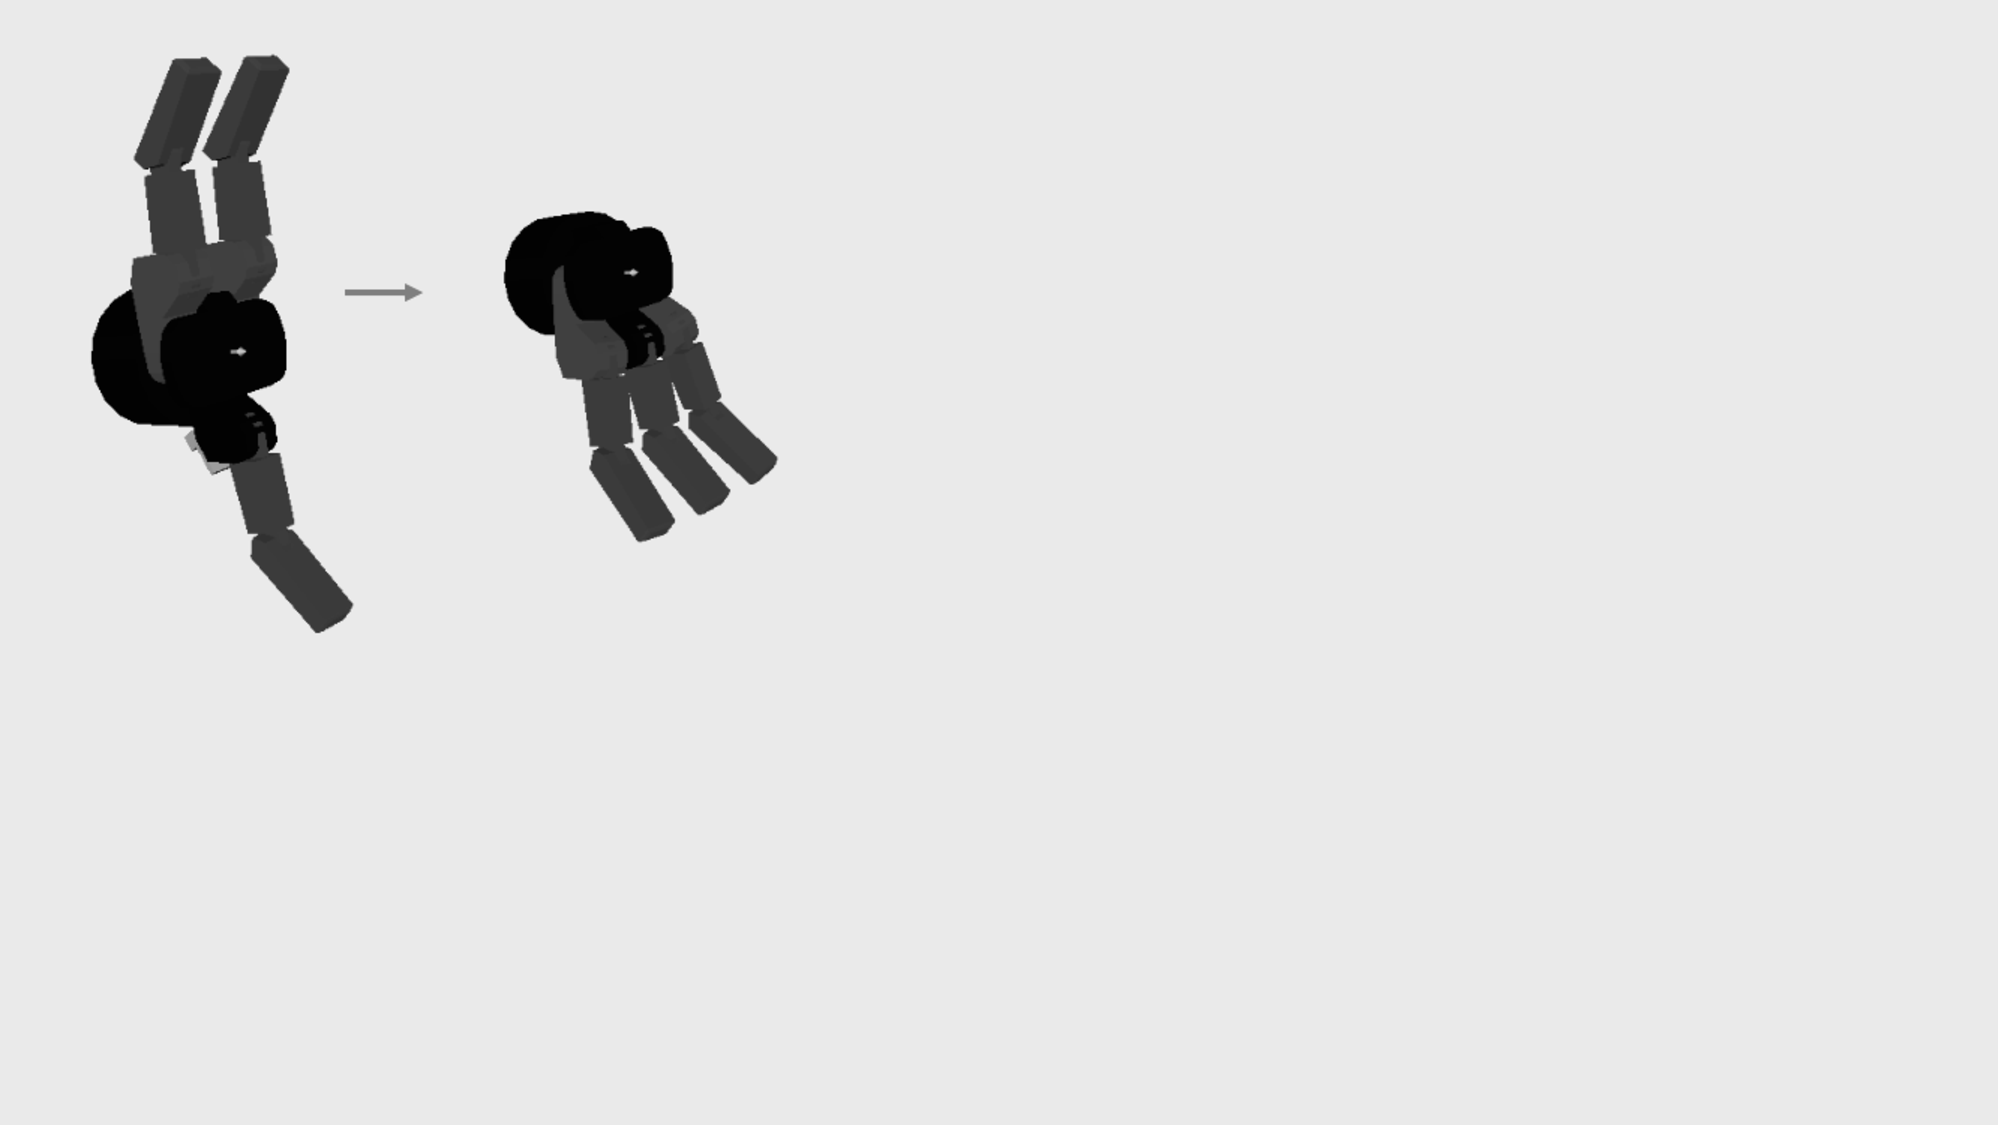
\includegraphics[trim={1cm 8cm 19cm 0cm},clip,width=1\linewidth,angle=0]{Apendices/Figuras/barret_eigengrasp_01.pdf}
				\caption{\textit{Eigengrasp} 01: fingers twist movement over wrist's normal axis.}
				\label{fig:barrett_eigengrasp01}
			\end{subfigure}
			\quad
			\begin{subfigure}[c]{.475\textwidth}
				\centering
				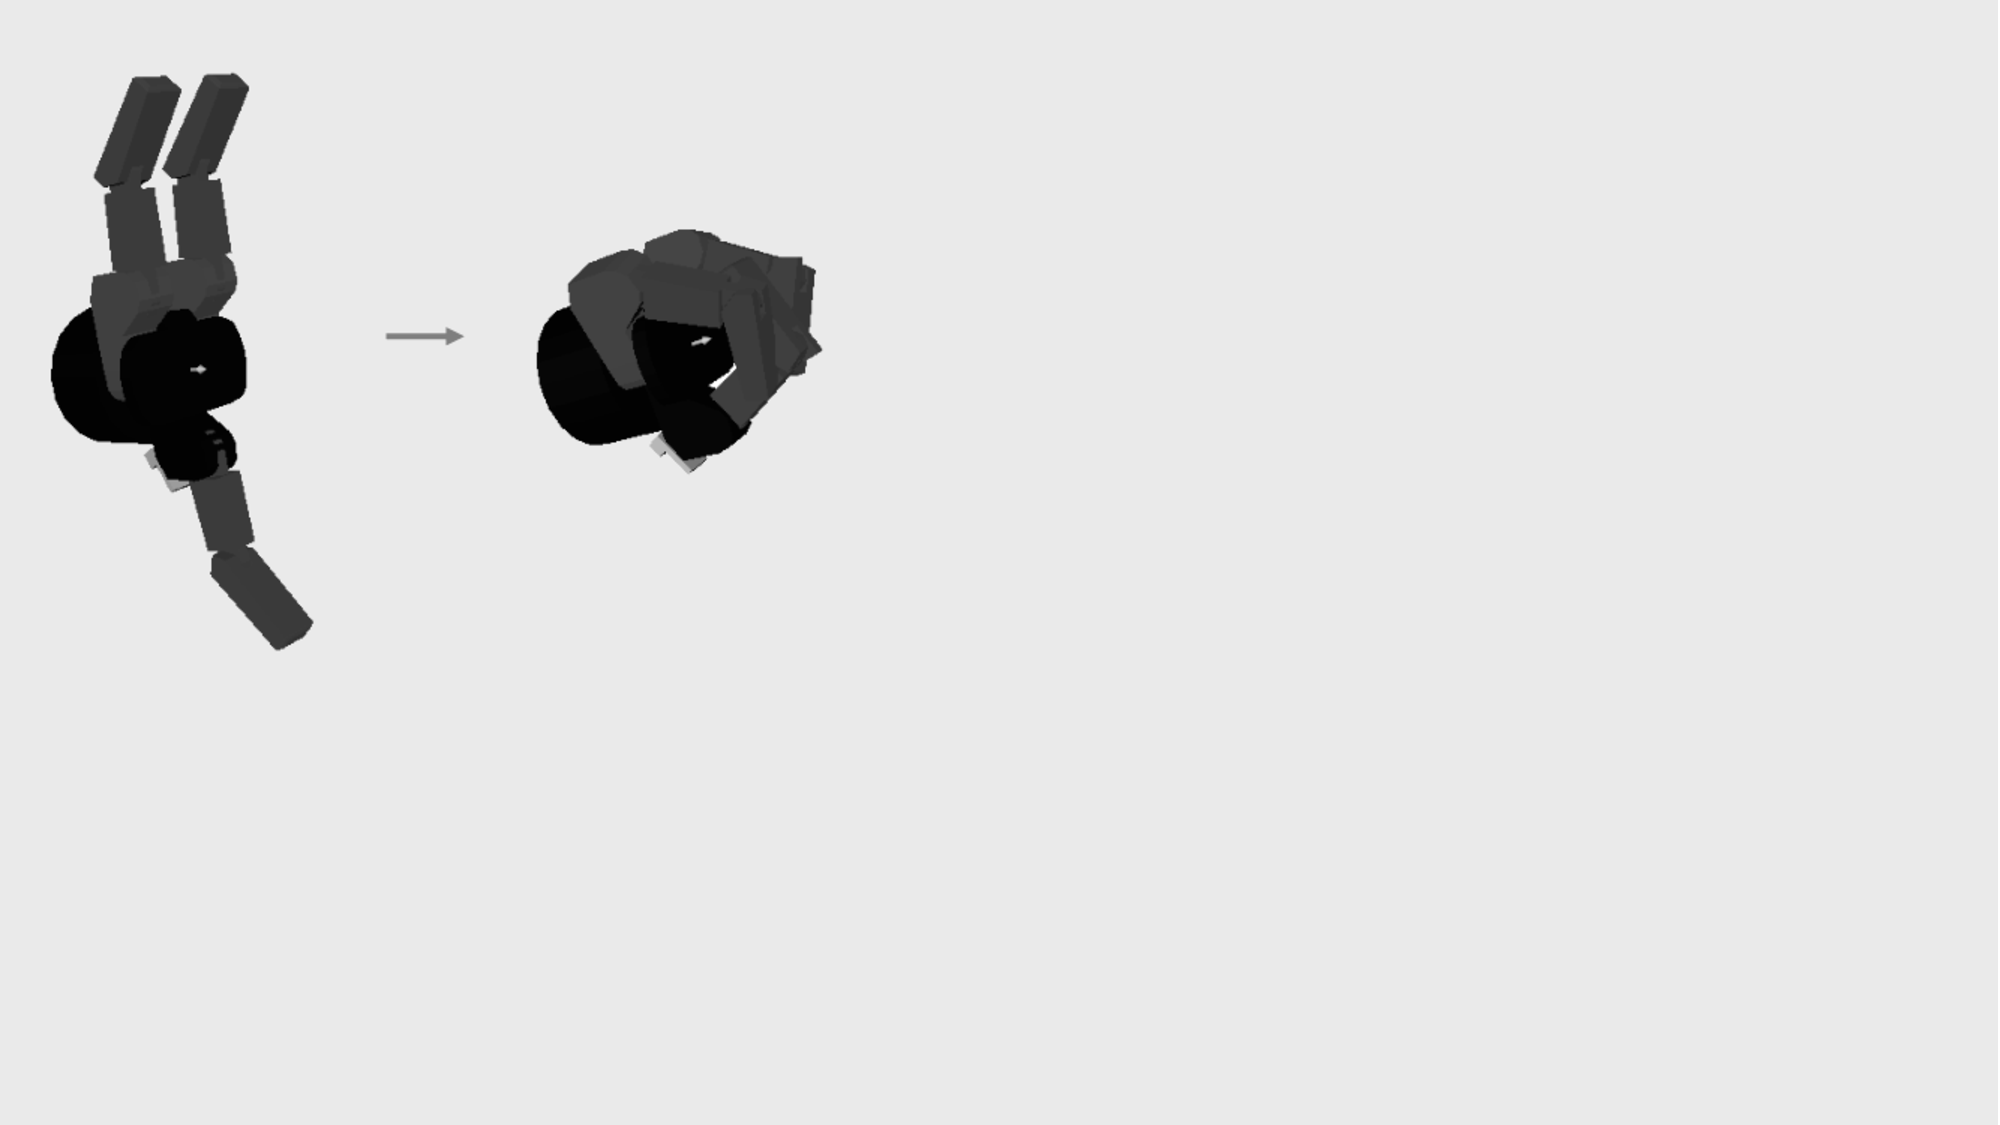
\includegraphics[trim={0.75cm 8cm 19cm 0.85cm},clip,width=1\linewidth,angle=0]{Apendices/Figuras/barret_eigengrasp_02.pdf}
				\caption{\textit{Eigengrasp} 02: fingers flexion.}
				\label{fig:barrett_eigengrasp02}
			\end{subfigure}
		\end{tcolorbox}
		\caption{The 4 \ac{DOF} Barrett gripper and its bidimensional \textit{eigengrasp} representation. }
		\label{fig:barrett_eigengrasps}
	}%end of resize box      
\end{figure}

The optimisation algorithm tries to minimize the distance from the \ac{ICP}, that constitute the \ac{ICR} (Figure~\ref{fig:icp_opt}), to the object surface by adjusting the discussed optimization variables $\mathbf{a}$ and $\mathbf{w}$. The \ac{ICR} is a contact region model (a predefined group of distributed \acp{ICP}) used to calculate the interaction of the algorithm, thus it is possible to create a feasible procedure. 

Therefore, the objective function to be minimised is describe by Equation~\ref{eq:fob_grasp_complete}, where $N$ is the number of total contacts in \ac{ICR}, $\mathbf{\hat{n}}_{i}$ is the surface normal, $\mathbf{o}_{i}$ the distance between the \ac{ICP} and the object ($i \in N$). The scalar $\alpha$ is a range adjustment factor between the distance and the normalised dot product of the second sum part. It is important to note that the $\mathbf{o}_{i}$ and $\mathbf{\hat{n}}_{i}$ are updated according to 3D simulation interaction in the ``GraspIt!''~\cite{AndrewT2004}. %A detailed description of the algorithm procedure is presented in \cite{Ciocarlie2009}.    

\begin{equation}
Q=\sum_{i=1}^{N}\left(1-\delta_{i}\right)\hspace{0.5cm}\textnormal{with}\hspace{0.5cm}\delta_{i}=\frac{\left|\mathbf{o}_{i}\right|}{\alpha}+\left(1-\frac{\mathbf{\hat{n}}_{i} \cdot\mathbf{o}_{i}}{\left|\mathbf{o}_{i}\right|}\right)
\label{eq:fob_grasp_complete}
\end{equation}


\begin{figure}[h!] %because of cas-sc
\resizebox{1\textwidth}{!}{%
\begin{tcolorbox}
% \centerline{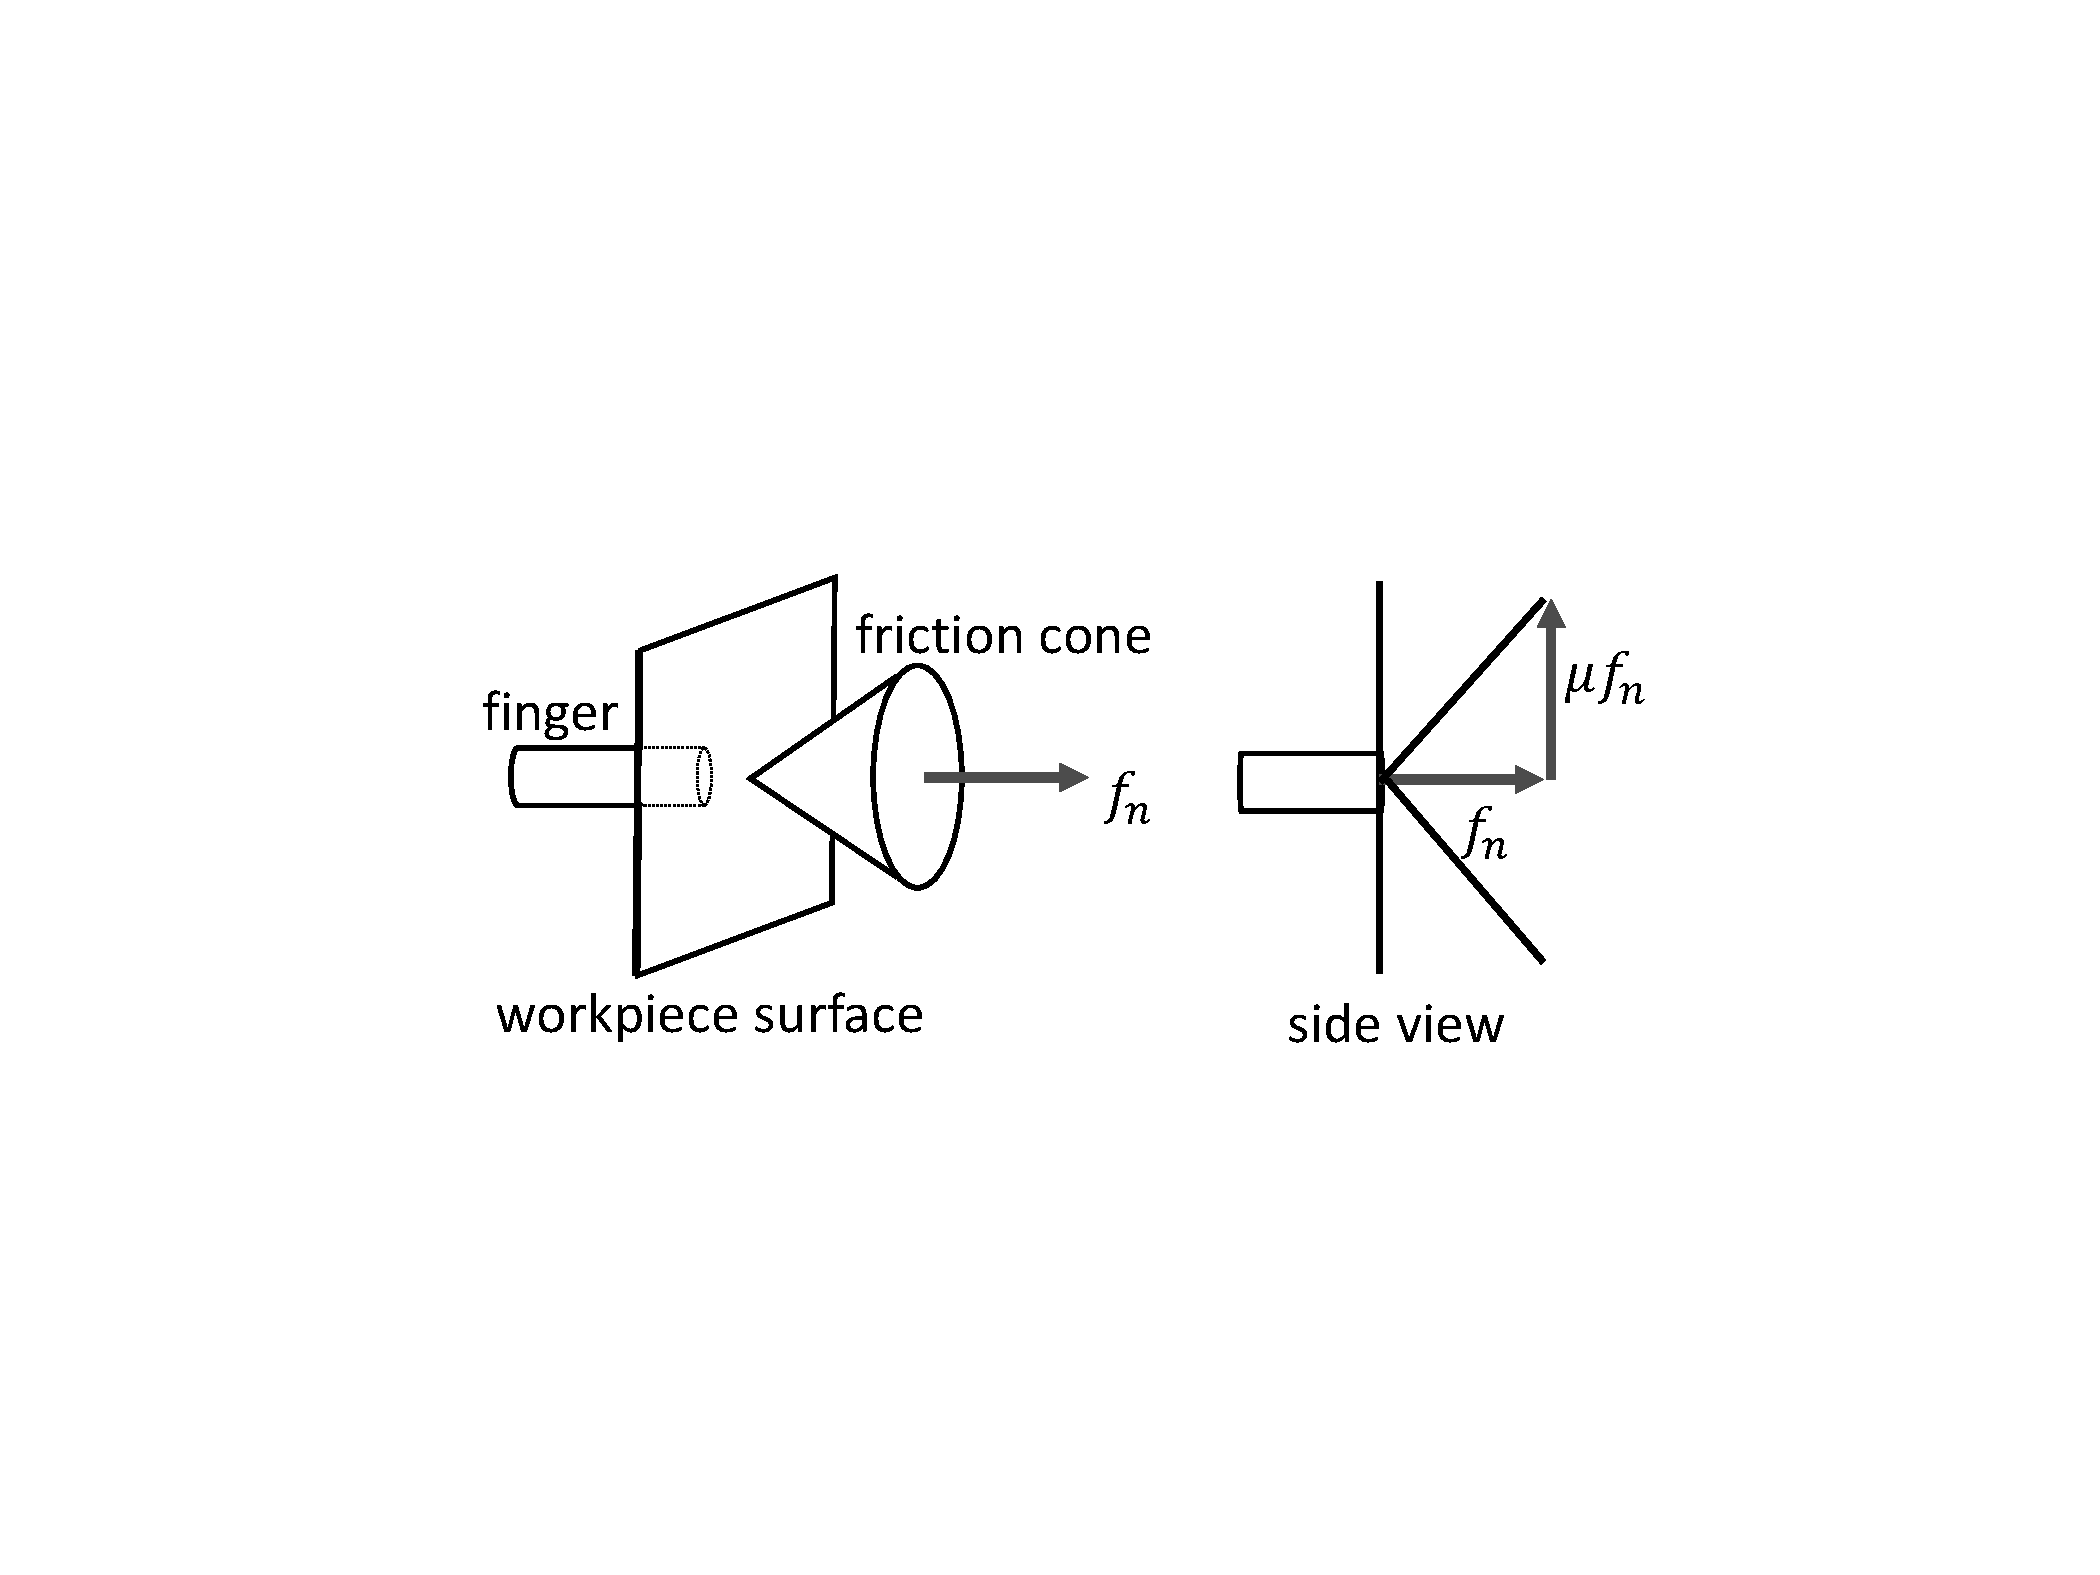
\includegraphics[trim={7cm 8cm 7cm 9cm},clip,width=1\linewidth,angle=0]{Cap2/Figuras/friction_contact.pdf}}
\centerline{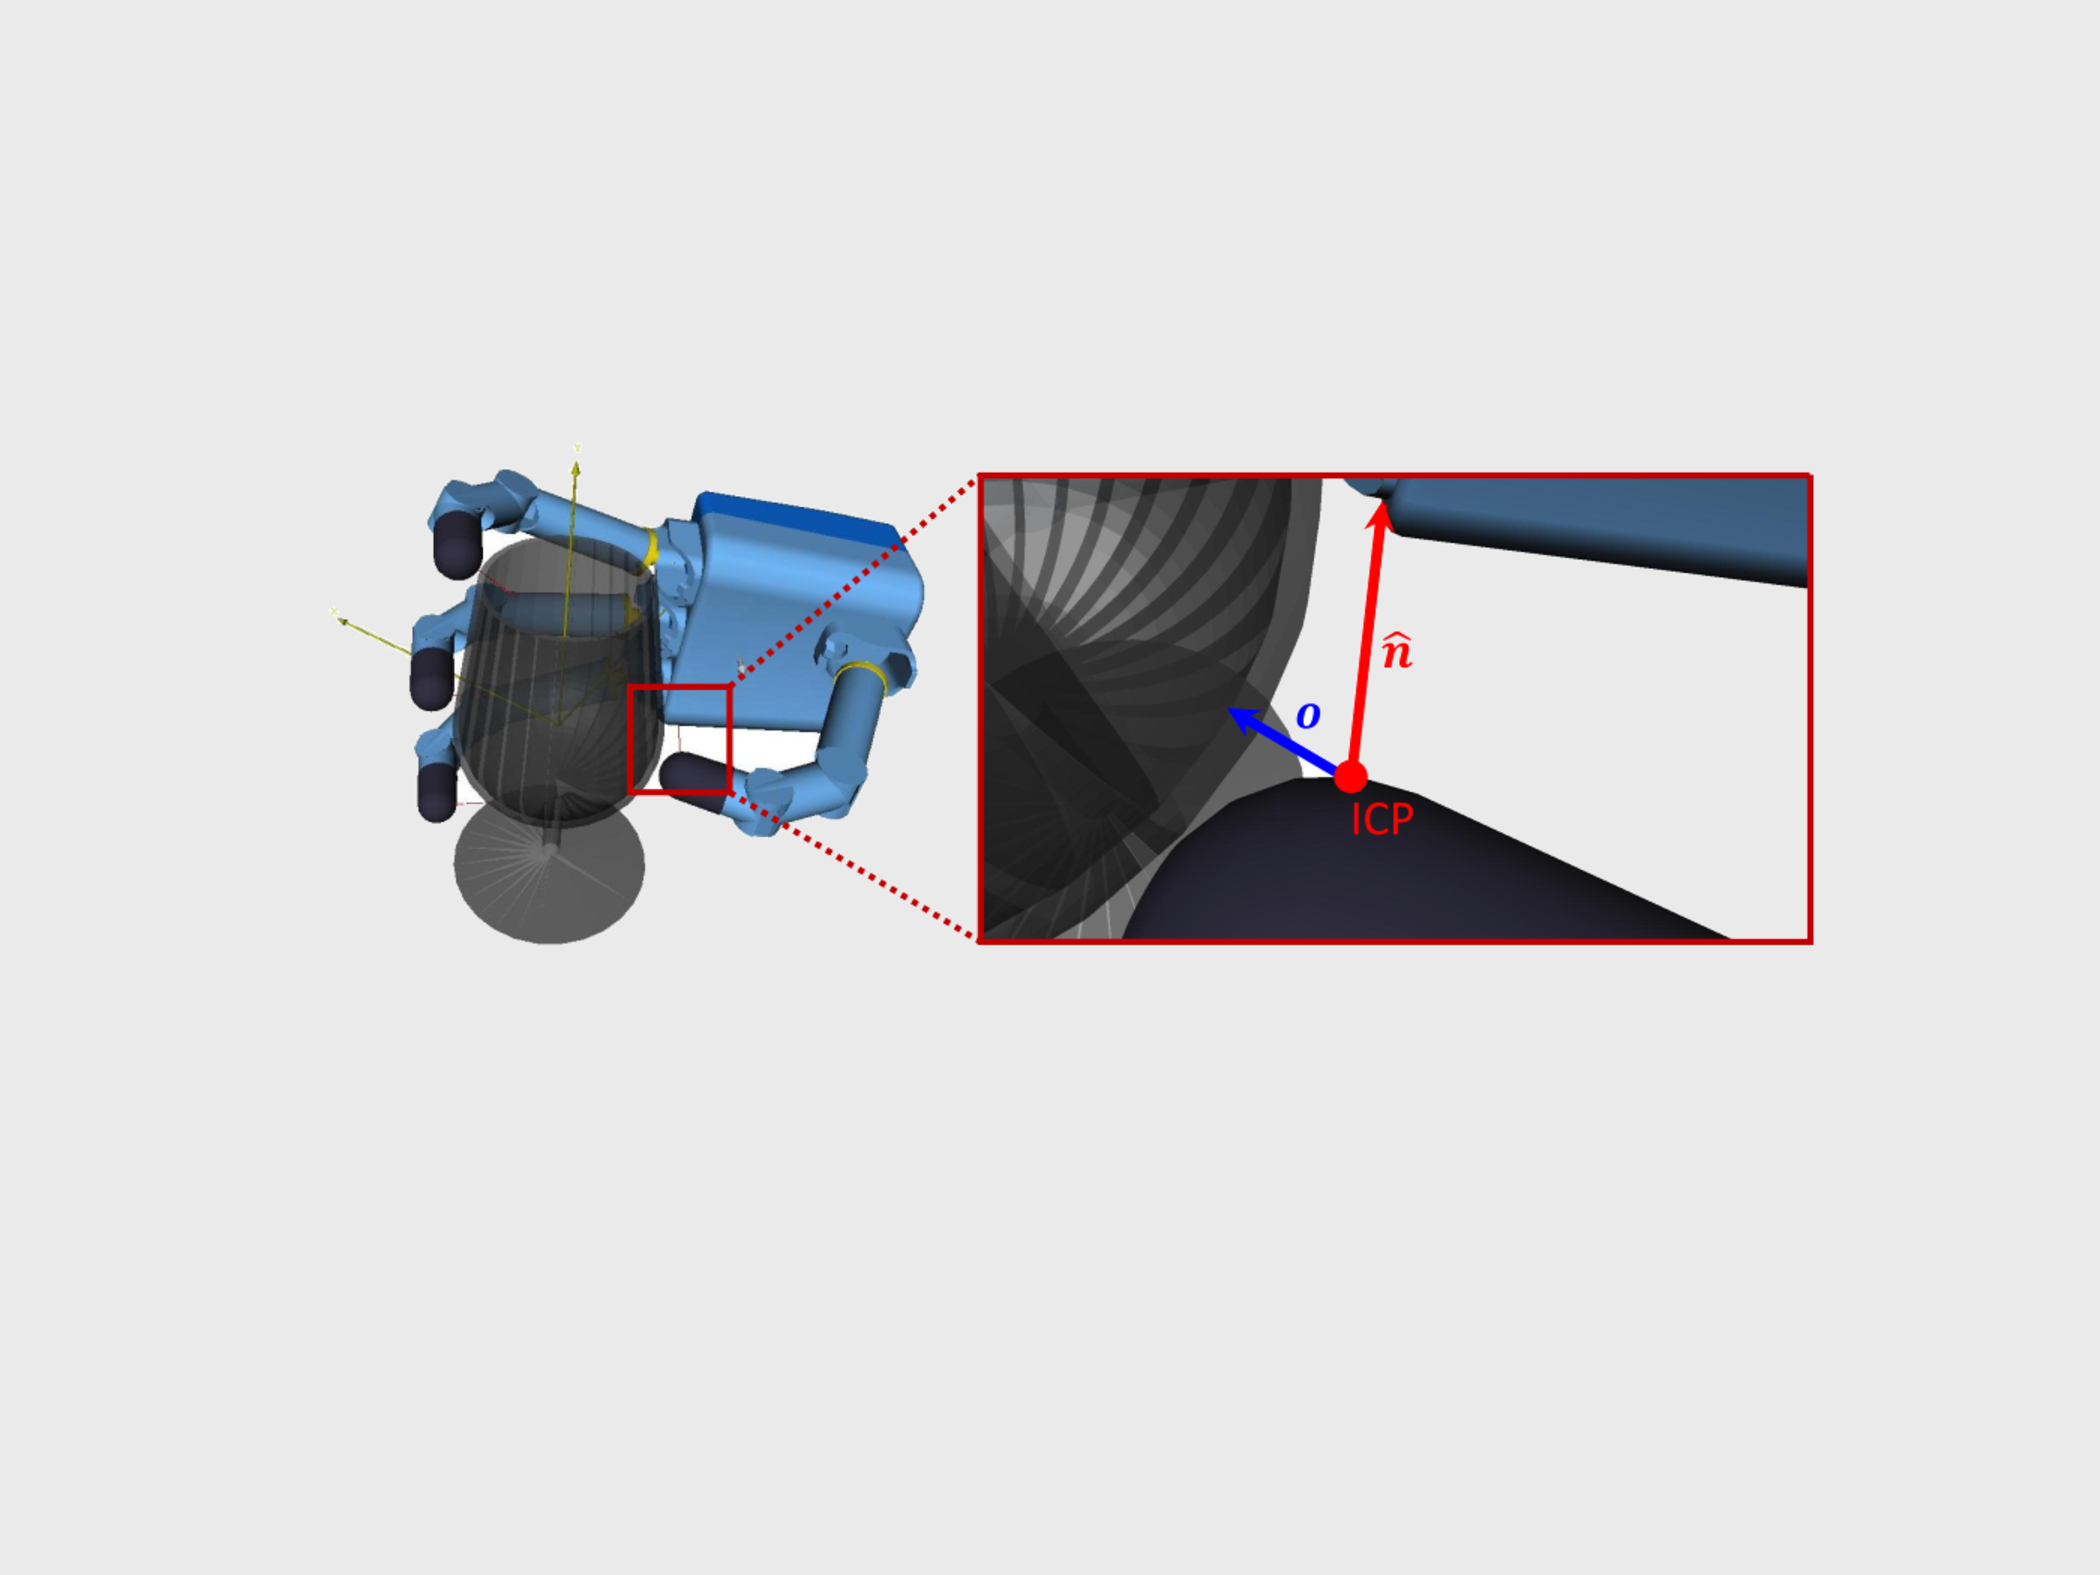
\includegraphics[trim={6.5cm 10cm 4cm 8cm},clip,width=1\linewidth,angle=0]{Apendices/Figuras/ICPreduction_gray_bg.pdf}}
\end{tcolorbox}
\caption{Grasping optimisation process elucidation.}
\label{fig:icp_opt}
}
\end{figure}


The algorithm proposed by~\cite{Ciocarlie2009}, and used in this proposal, is replicated in Algorithm~\ref{alg:snn_grasp}. As already mentioned, the variables that define the states are $\mathbf{a}$, related to the \textit{eigengrasp}, and $\mathbf{w}$, related to the wrist pose. The ``\textit{ObjFunc}'' is described by Equation~\ref{eq:fob_grasp_complete}. The ``\textit{Ngbr}'' is the calculus of the state variables neighbout valuer using the Equation~\ref{eq:neighbors} and, ``\textit{Probability}'' is the function to perform the jump probability to a new state according to Equation~\ref{eq:very_fast_snn_prob}. Since this step of the algorithm is based on ``GraspIt!''} the ``ForwardKinematics'' and collision check are are parts of this tool.

 \begin{algorithm}[h!]
 	\centering
	\resizebox{0.85\textwidth}{!}{%
	\begin{tcolorbox}
		\ForAll {variables of CurrentState} 
		{CurrentState.variable = RandomValue()}
		QCurrent = ObjFunc(CurrentState)\;
		Steps = 0\;
		QSaved = 0\;
		\While{Steps $\neq$ MaxSteps}{
			{Generate a new state as a neighbor of current state}\;
			\Repeat{legalState == true}
			{
				\ForAll{variables of NewState}{
					Sim. Annealing neighbor generation function\;
					NewState.variable = Ngbr(CurrentState.variable)\;
				}
				Apply ForwardKinematics(NewState)\;
				\If{collisions detected \textnormal{\textbf{or}} joint limits exceeded} {
					legalState = false\;
				} \Else{
					legalState = true
				}
				
			} 
			QNew = ObjFunc(NewState)\;
			\If{QNew $>$ QSaved}
			{
				Insert NewState in SavedStatesList\;
				QSaved = lowest ObjFunc value in SavedStateList\;
			}
			Sim. Annealing probability of "jumping" to new state\;
			PJump = Probability(QCurrent, QNew)\;
			\If{PJump $>$ 0.5}{
				CurrentState = NewState\;
				QCurrent = QNew\;
			}
			Steps = Steps + 1\;
		}	
		 \end{tcolorbox}
		\caption{\ac{SANN} applied to grasping}
		\label{alg:snn_grasp}
		}
\end{algorithm}

%-----------------------------------------------------------------------------------------------------------------
\chapter{Related Work}
\label{cap2:related_work}

%-------------------------------------------------------------------------------------------------------------
Given the vast range of works in the robotic grasping, this chapter discusses and reviews state-of-the-art proposals of grasping solutions and how they evolved over the years. This chapter build the basis to the thesis proposals.

%It also discusses and presents the new steps and future works ideas not yet explored: from the academic field to the new challenges of industry 4.0. 

%Moreover, the first Ph.D contribution is presented. It formalises and standardises the grasping evaluation idea since a grasping problem involves perception, planning, and control. Therefore, a clear standard could improve the methodologies' comparability since each step of the procedure affects the grasping performance. 

The remainder of the chapter is organised as follows: Section~\ref{cap2:related_work:sec:grasping_representation} shows and discusses the different grasping representations since the characterisation is the most important step to any grasping planning approach. A review of Analytical, Learning and Deep Learning methods is given in Sections~\ref{cap2:related_work:sec:grasping_approaches:subsec:analytical_review}, \ref{cap2:related_work:sec:grasping_approaches:subsec:learning_review}, and \ref{cap2:related_work:sec:grasping_approaches:subsec:deep_learning_review}, respectively.

%Section~\ref{sec:grasping_evaluation} presents a grasping evaluation discussion following by our proposal.  The discussion, exploration of future works ideas, and the conclusion are presented in Sections~\ref{sec:discussion_and_future_work}, and ~\ref{sec:conclusion}, respectively. 


%The rest of the paper is divided as follow: after the introduction section, a grasping definition %problem is introduced in Section~\ref{sec:grasping_definition_problem}, formalizing the discussion %along the paper. Section~\ref{sec:grasping_representation} shows and discuss the types of grasping %representation. A review about Analytical, Learning and Deep Learning methods are given in %Sections~\ref{sec:analytical_review}, \ref{sec:learning_review} and \ref{sec:deep_learning_review}, %respectively. The Section~\ref{sec:grasping_evaluation} presents a grasping evaluation discussion %following by our proposal.  In the end, the conclusion is presented in Section~\ref{sec:conclusion} %exploring future works ideas. 


% \section{The Robotic Grasping Problem}\label{sec:grasping_definition_problem}

% The robotic grasping affordance is related to perform a set of contacts (or stay near, in the case of magnetic and suction gripper) between the active pairs (the workpiece and the gripper). Typically, as related by~\cite{Ghazaei2019}, a grasping procedure can be divided in three parts: perception, planning and control. An detailed example description of this common proposal is presented in the Figure~\ref{fig:grasping}. 


%\begin{figure}[h]
%    \centering
%    \includegraphics[scale=0.5]{example-image-a} 
%    \caption{XXX}
%    \label{fig:grasping}
%\end{figure}{}



\section{Grasping Representation}
\label{cap2:related_work:sec:grasping_representation}


There are several approaches regarding how to represent a grasping, i.e., how to describe and characterise it. This subject is a valuable step to the development of grasping planning or grasping detection algorithms and will be discussed in this section.  


Some approaches model the physical interaction between the active pairs and evaluate its equilibrium and stability performance with the wrench space analyses and Coulomb's law in multi-fingered grasping (Figure~\ref{fig:friction_contact}). It is a prevalent approach in analytical methodologies~\cite{liu2004complete,el2009computing, miller2004graspit, AndrewT2004} and present in Learning and \ac{DL} policies~\cite{Mahler2016, Mahler2017b, Mahler2017d, Mahler2017, Mahler2019}. Typically, it depends on the active pair's 3D shape (Point-Cloud, Voxel Grids, or 3D models) since the contacts need to be evaluated in an iteration algorithm or simulation. Well-recognised quality metrics are the Convex Hull's volume and the Epsilon radius of the grasping wrench space configuration proposed by \citeauthor{Ferrari} in~\cite{Ferrari} (Figure~\ref{fig:gws_force_closure_main}). Since a complete wrench space analyses  demand effort, a simplified modelling strategy is the antipodal restraints~\cite{Nguyen1987_1} represented by Figure~\ref{fig:antipodal}, which is commonly used by proposals that employ two-finger grasping. 

\begin{figure}[h!] %because of cas-sc
\resizebox{.7\textwidth}{!}{%
\begin{tcolorbox}
\centerline{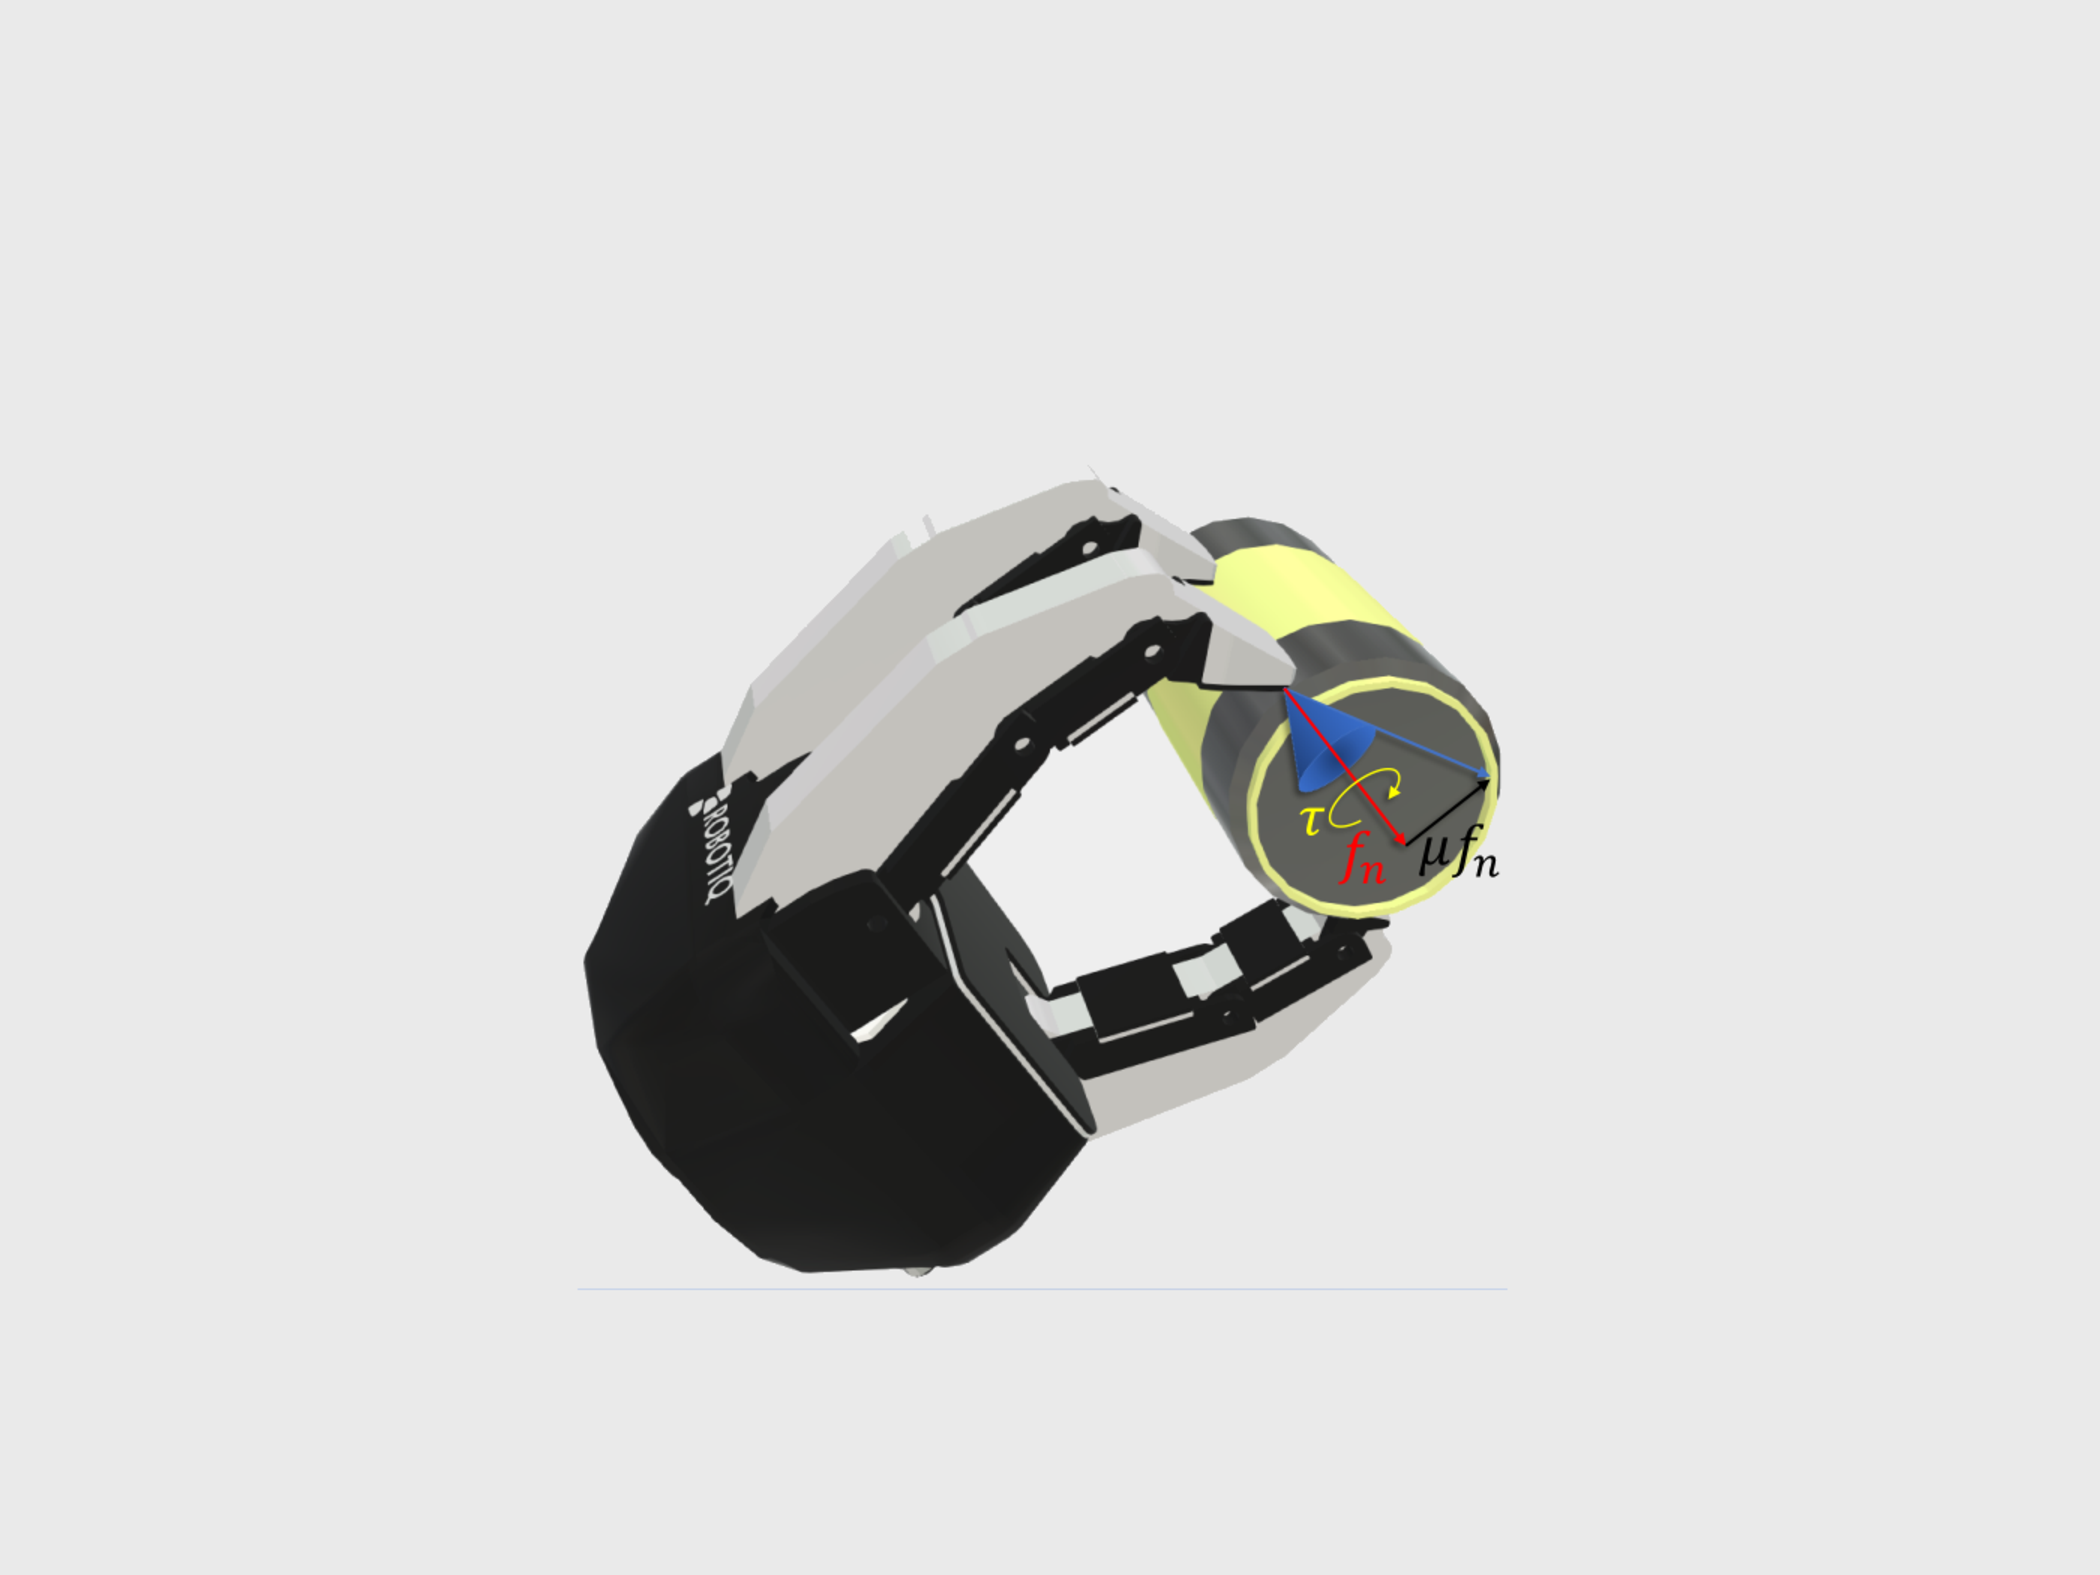
\includegraphics[trim={10cm 5cm 10.2cm 8cm},clip,width=.75\linewidth,angle=0]{Cap2/Figuras/grasp.pdf}}
\end{tcolorbox}
\caption{Soft finger friction contact model.}
\label{fig:friction_contact}
\label{fig:}
}
\end{figure}



% \begin{figure}[h]
%     \centering
%     \includegraphics[scale=0.5]{example-image-a} 
%     \caption{Wrench space analyses and Coulomb’s law}
%     \label{fig:wrench_space_coulombs_theory}
% \end{figure}

% \begin{figure}[h]
%     \centering
%     \includegraphics[scale=0.5]{example-image-a} 
%     \caption{Convex Hull's Epsilon and Volume grasping representation: normally the task is to find the finger's poses over the object and evaluate the epsilon and volume values.}
%     \label{fig:epsilon_and_volume}
% \end{figure}


% \begin{figure}[h!] %because of cas-sc
% % \centerline{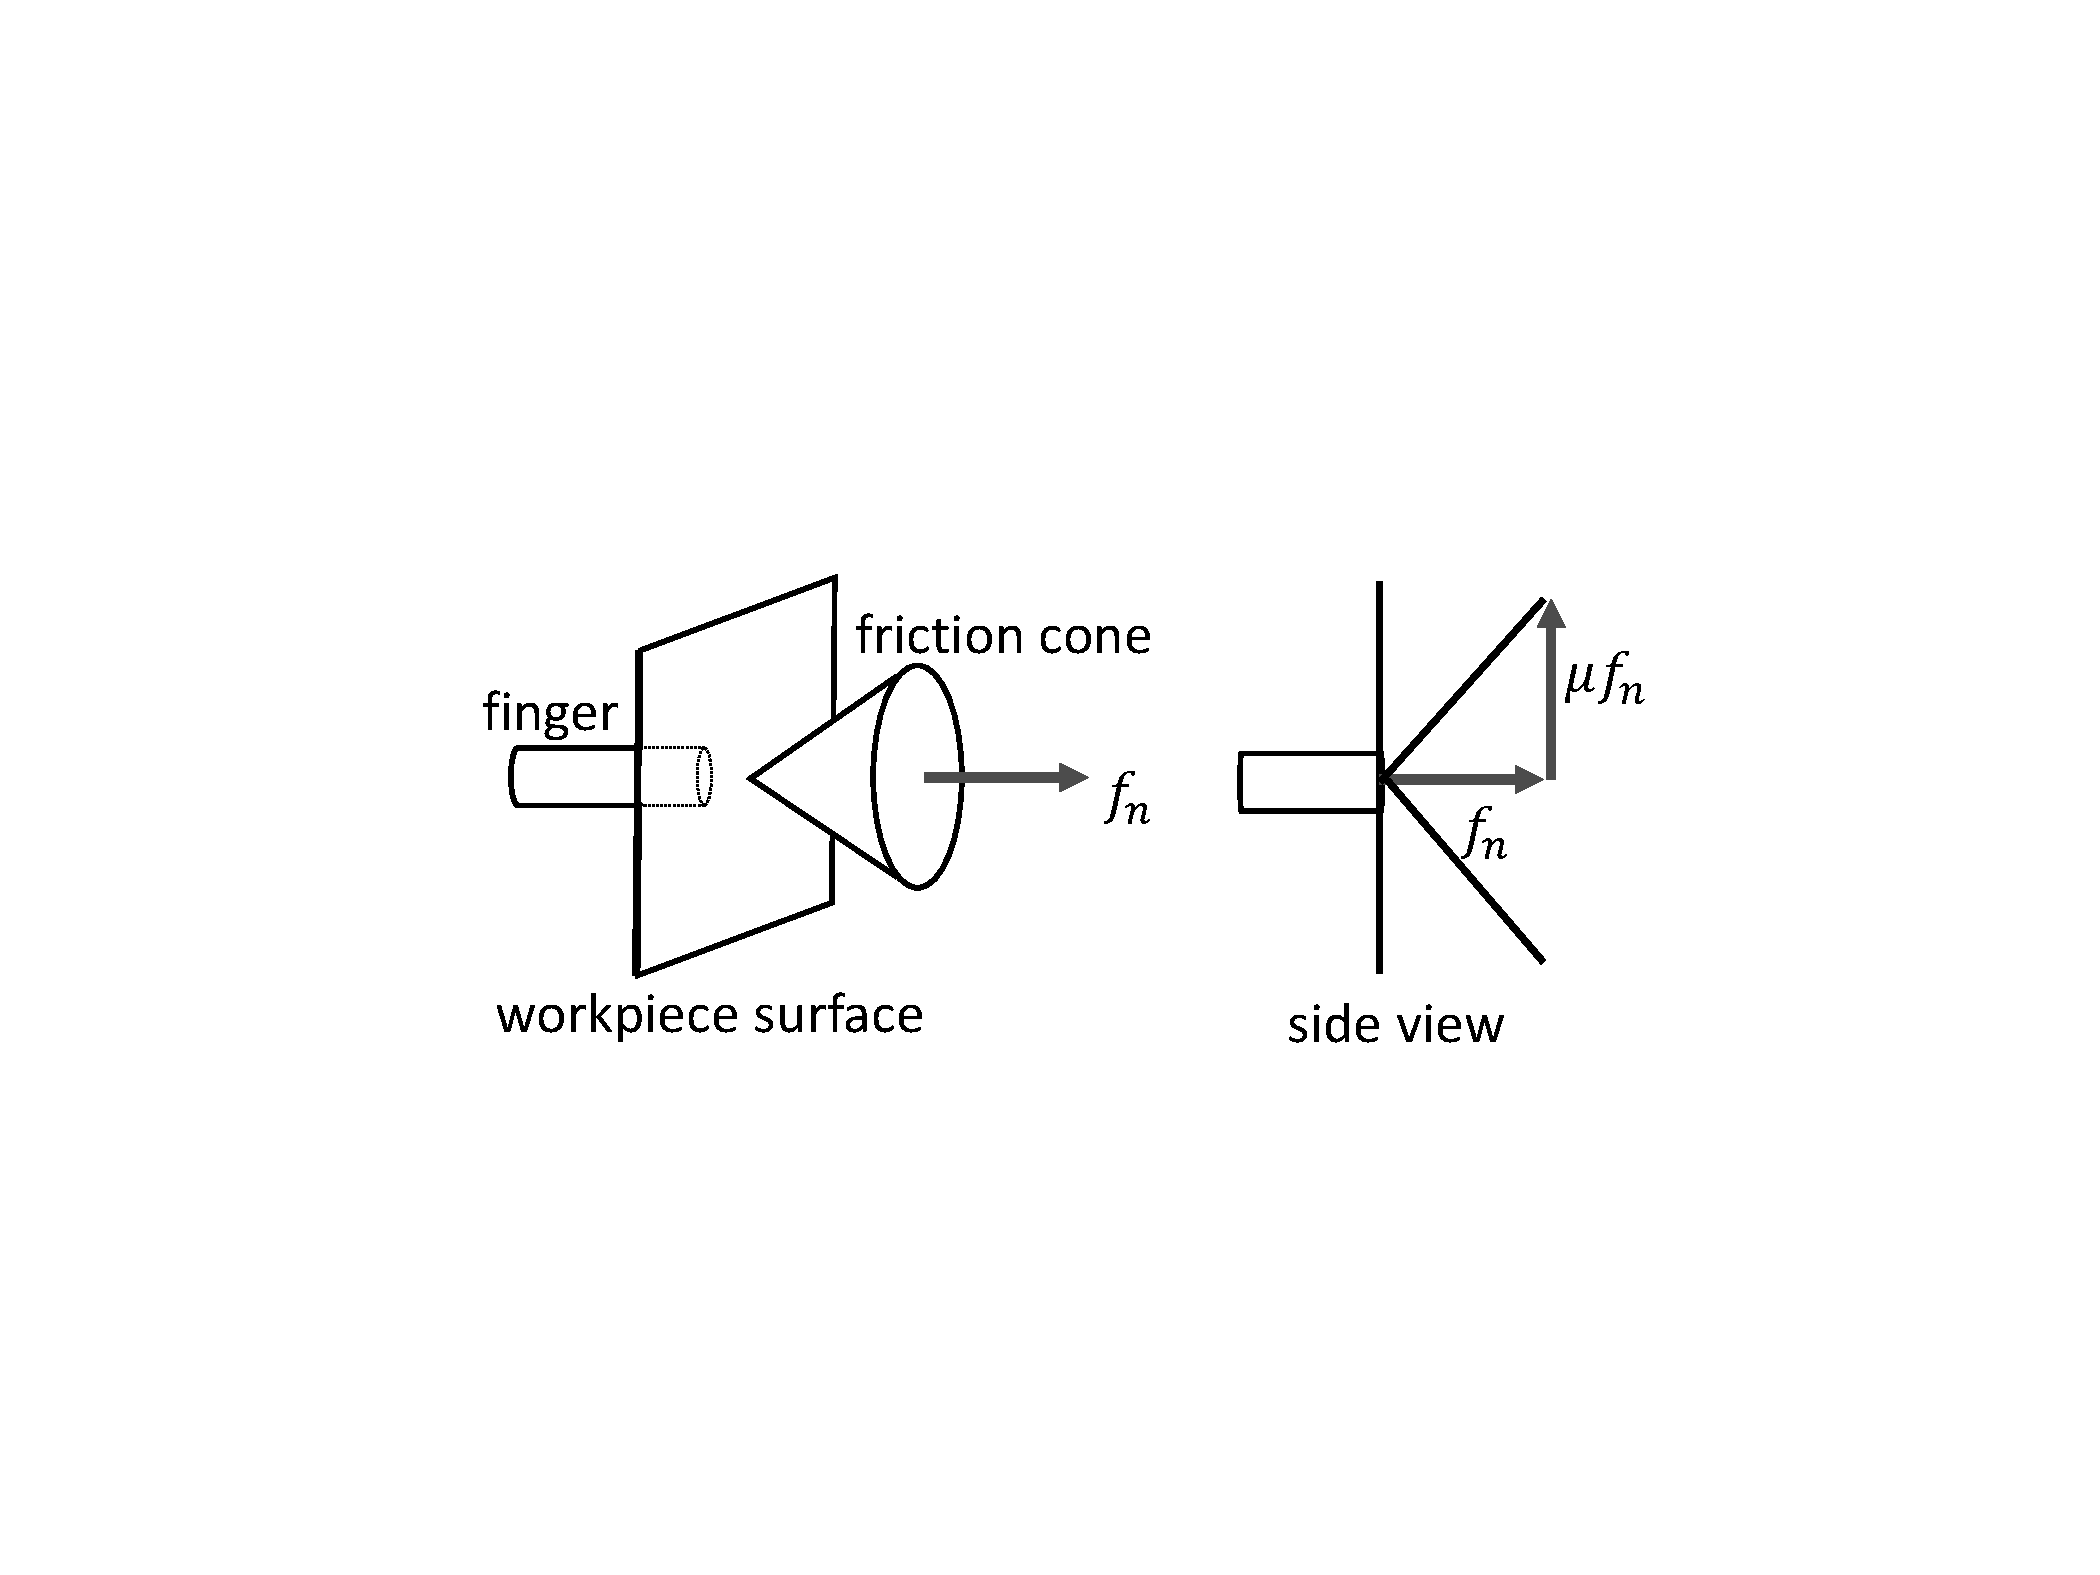
\includegraphics[trim={7cm 8cm 7cm 9cm},clip,width=1\linewidth,angle=0]{Cap2/Figuras/friction_contact.pdf}}
% \centerline{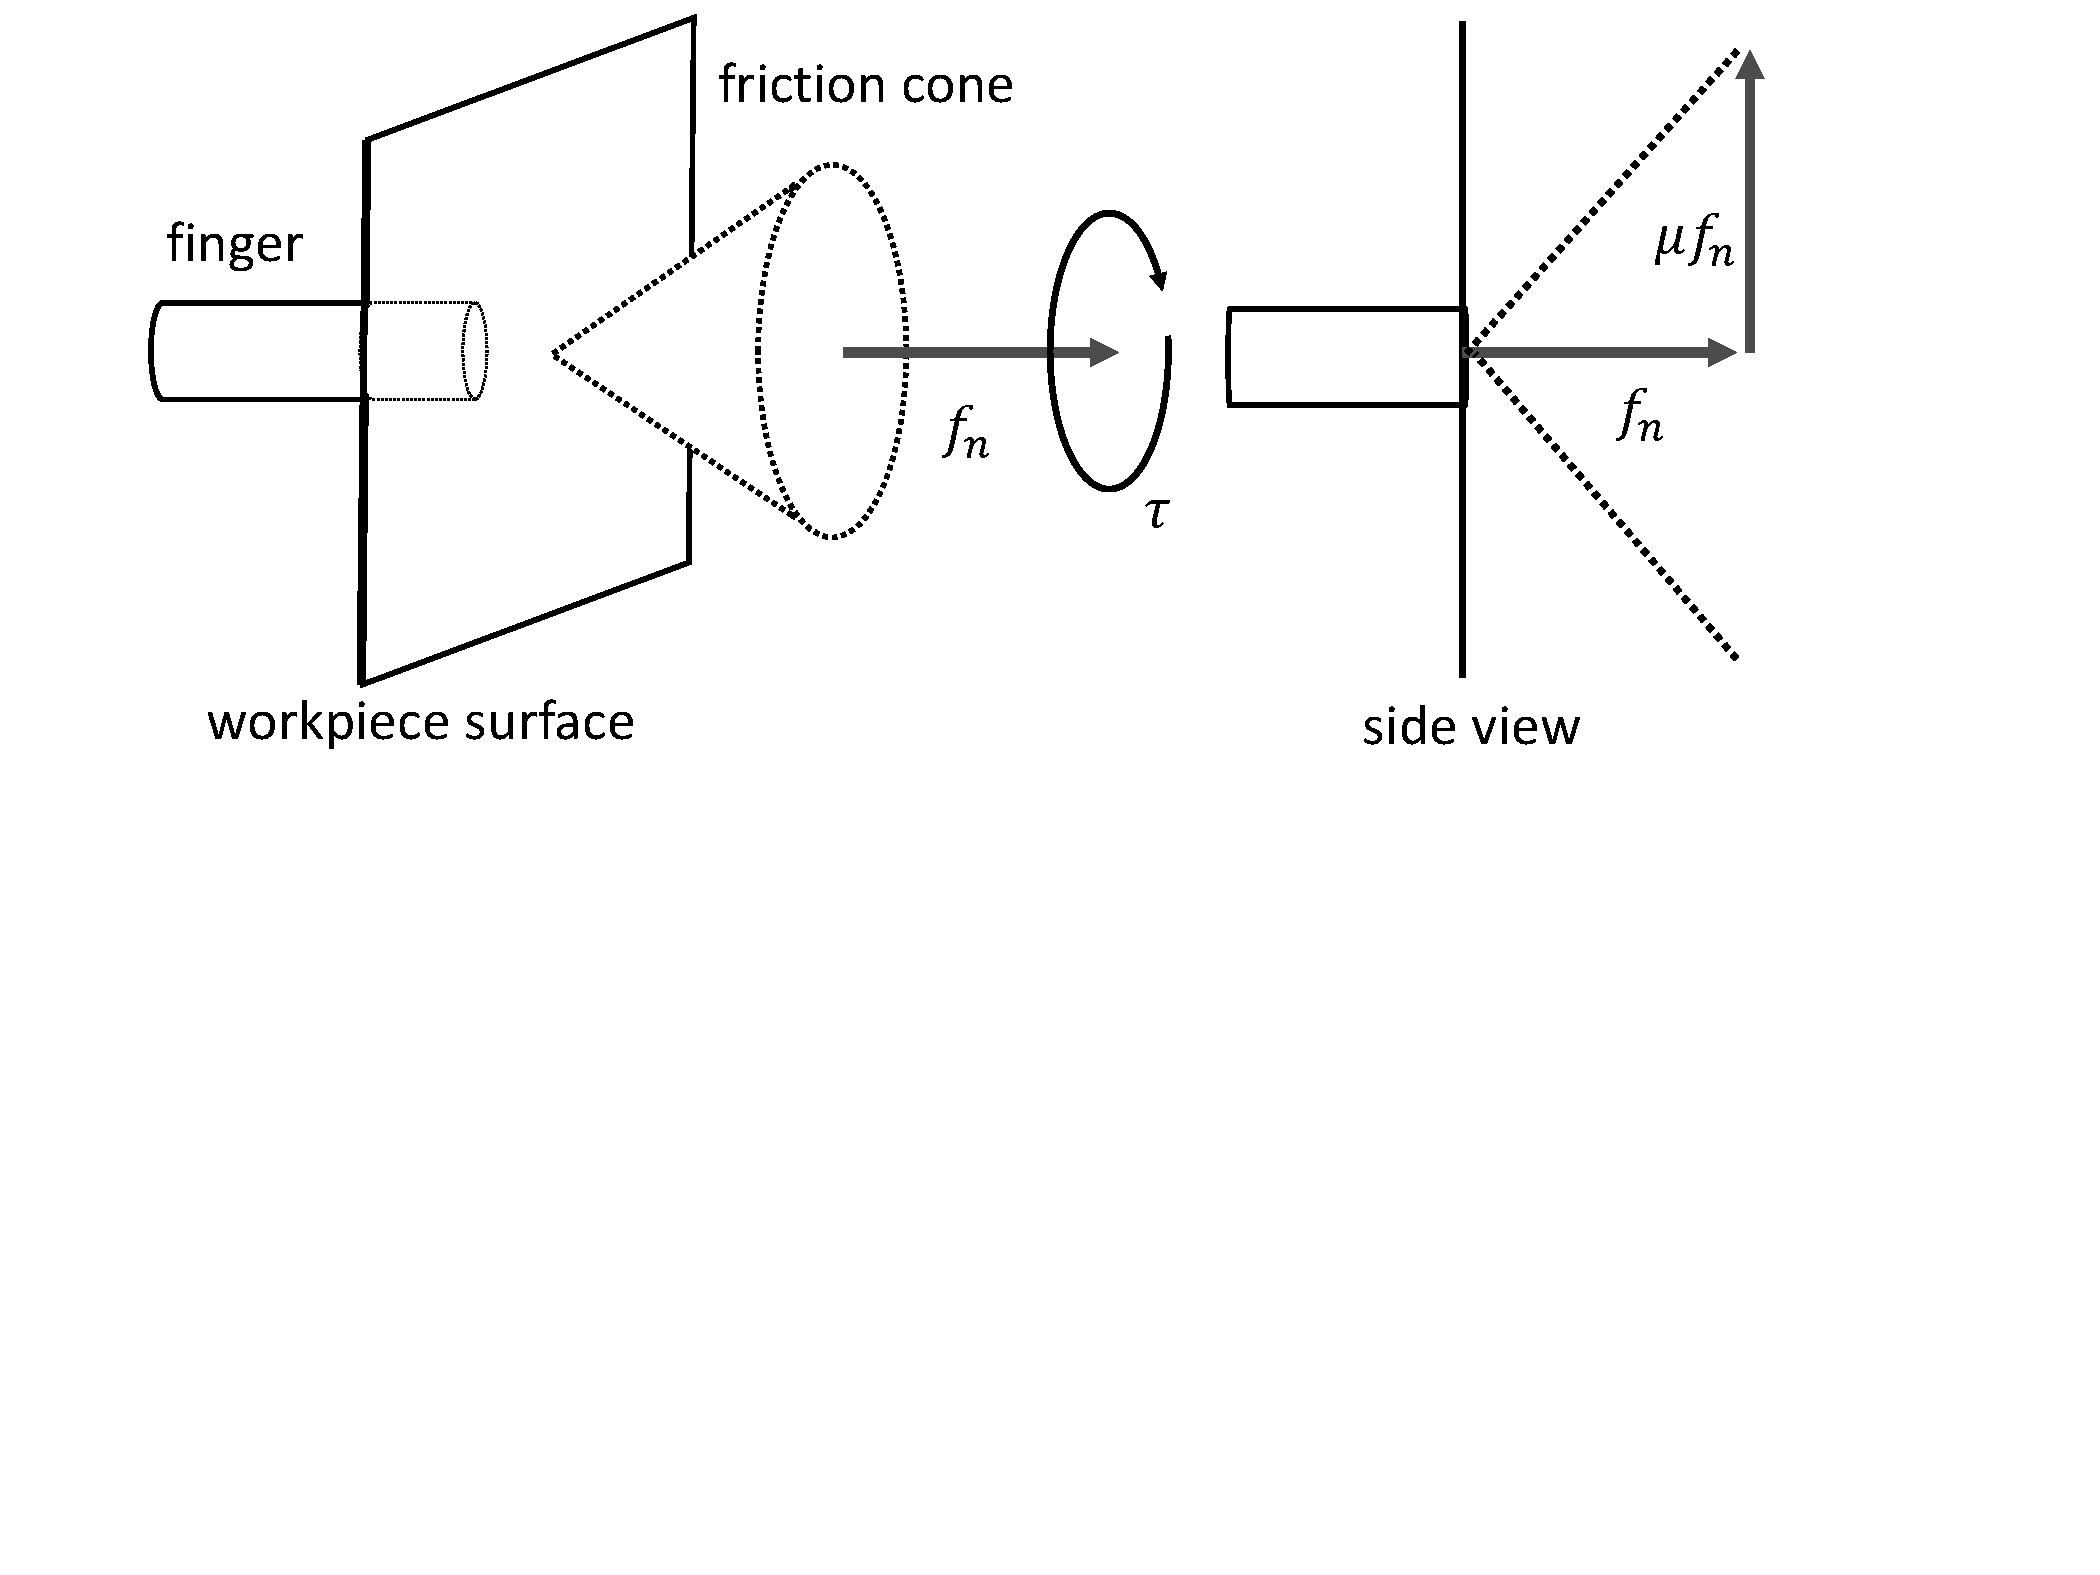
\includegraphics[trim={2.5cm 14cm 5.7cm 0cm},clip,width=.85\linewidth,angle=0]{Cap2/Figuras/soft_finger_contact.pdf}}
% \caption{A soft friction contact model and the geometric representation of Coulomb’s law (figure based on~\cite{murray1994mathematical}). }
% \label{fig:friction_contact}
% \end{figure}


In many applications,  the model shapes unfamiliarity is a significant drawback, and the ability to exceed the grasping to novel objects is necessary. This capability is also referred to as object-agnostic grasping. Decomposition heuristics and learning algorithms try to solve this issue. Even though, in most cases, the gripper topology generalisation is not considered. The point~\cite{Saxena2008} and the oriented rectangle grasping representations~\cite{Jiang2011a} (Figure~\ref{fig:exemples_rep}) were the options of several works to find a grasping pose over an object. These metrics, used in \ac{SL} methodologies, commonly require a labelled ground-truth, as \ac{CGD}~\cite{conerll_database} and Jacquard~\cite{jacquard_dataset} datasets. The point representation, normally indicated by a 3D pose, has a lack of physical limitation descriptors, like gripper's width and orientation approach angle, which are included in the rectangle methodology, see Figure~\ref{fig:exemples_rep}. The point representation metric only evaluates a distance between the detected grasping pose and the ground-truth, while the rectangle is also evaluated by the Jacquard threshold (Figure~\ref{fig:pen_jacquard}).


\begin{tcolorbox}[every float=\centering, drop shadow, title= Wrench Space Analyses]
Each contact can be modelled by a wrench vector $\mathbf{w}$ composed of forces and torques. All contact wrenches associated mould the convex-hull configuration, which can evaluate a grasping equilibrium. In a case of planar multi-fingered grasp, a force-closure grasp has the wrench space origin included by its convex-hull geometry (left convex-hull of Figure~\ref{fig:gws_force_closure_main}), unlike a non-force closure (right convex-hull of Figure~\ref{fig:gws_force_closure_main}). The $\epsilon$ is an example of the quality value to define the best force-closure configuration. It represents the wrench vector's distance to the origin ($\{O\}$), which is the shortest, i.e., the worst wrench vector to support an external perturbation.

\vspace*{1ex}

% \centerline{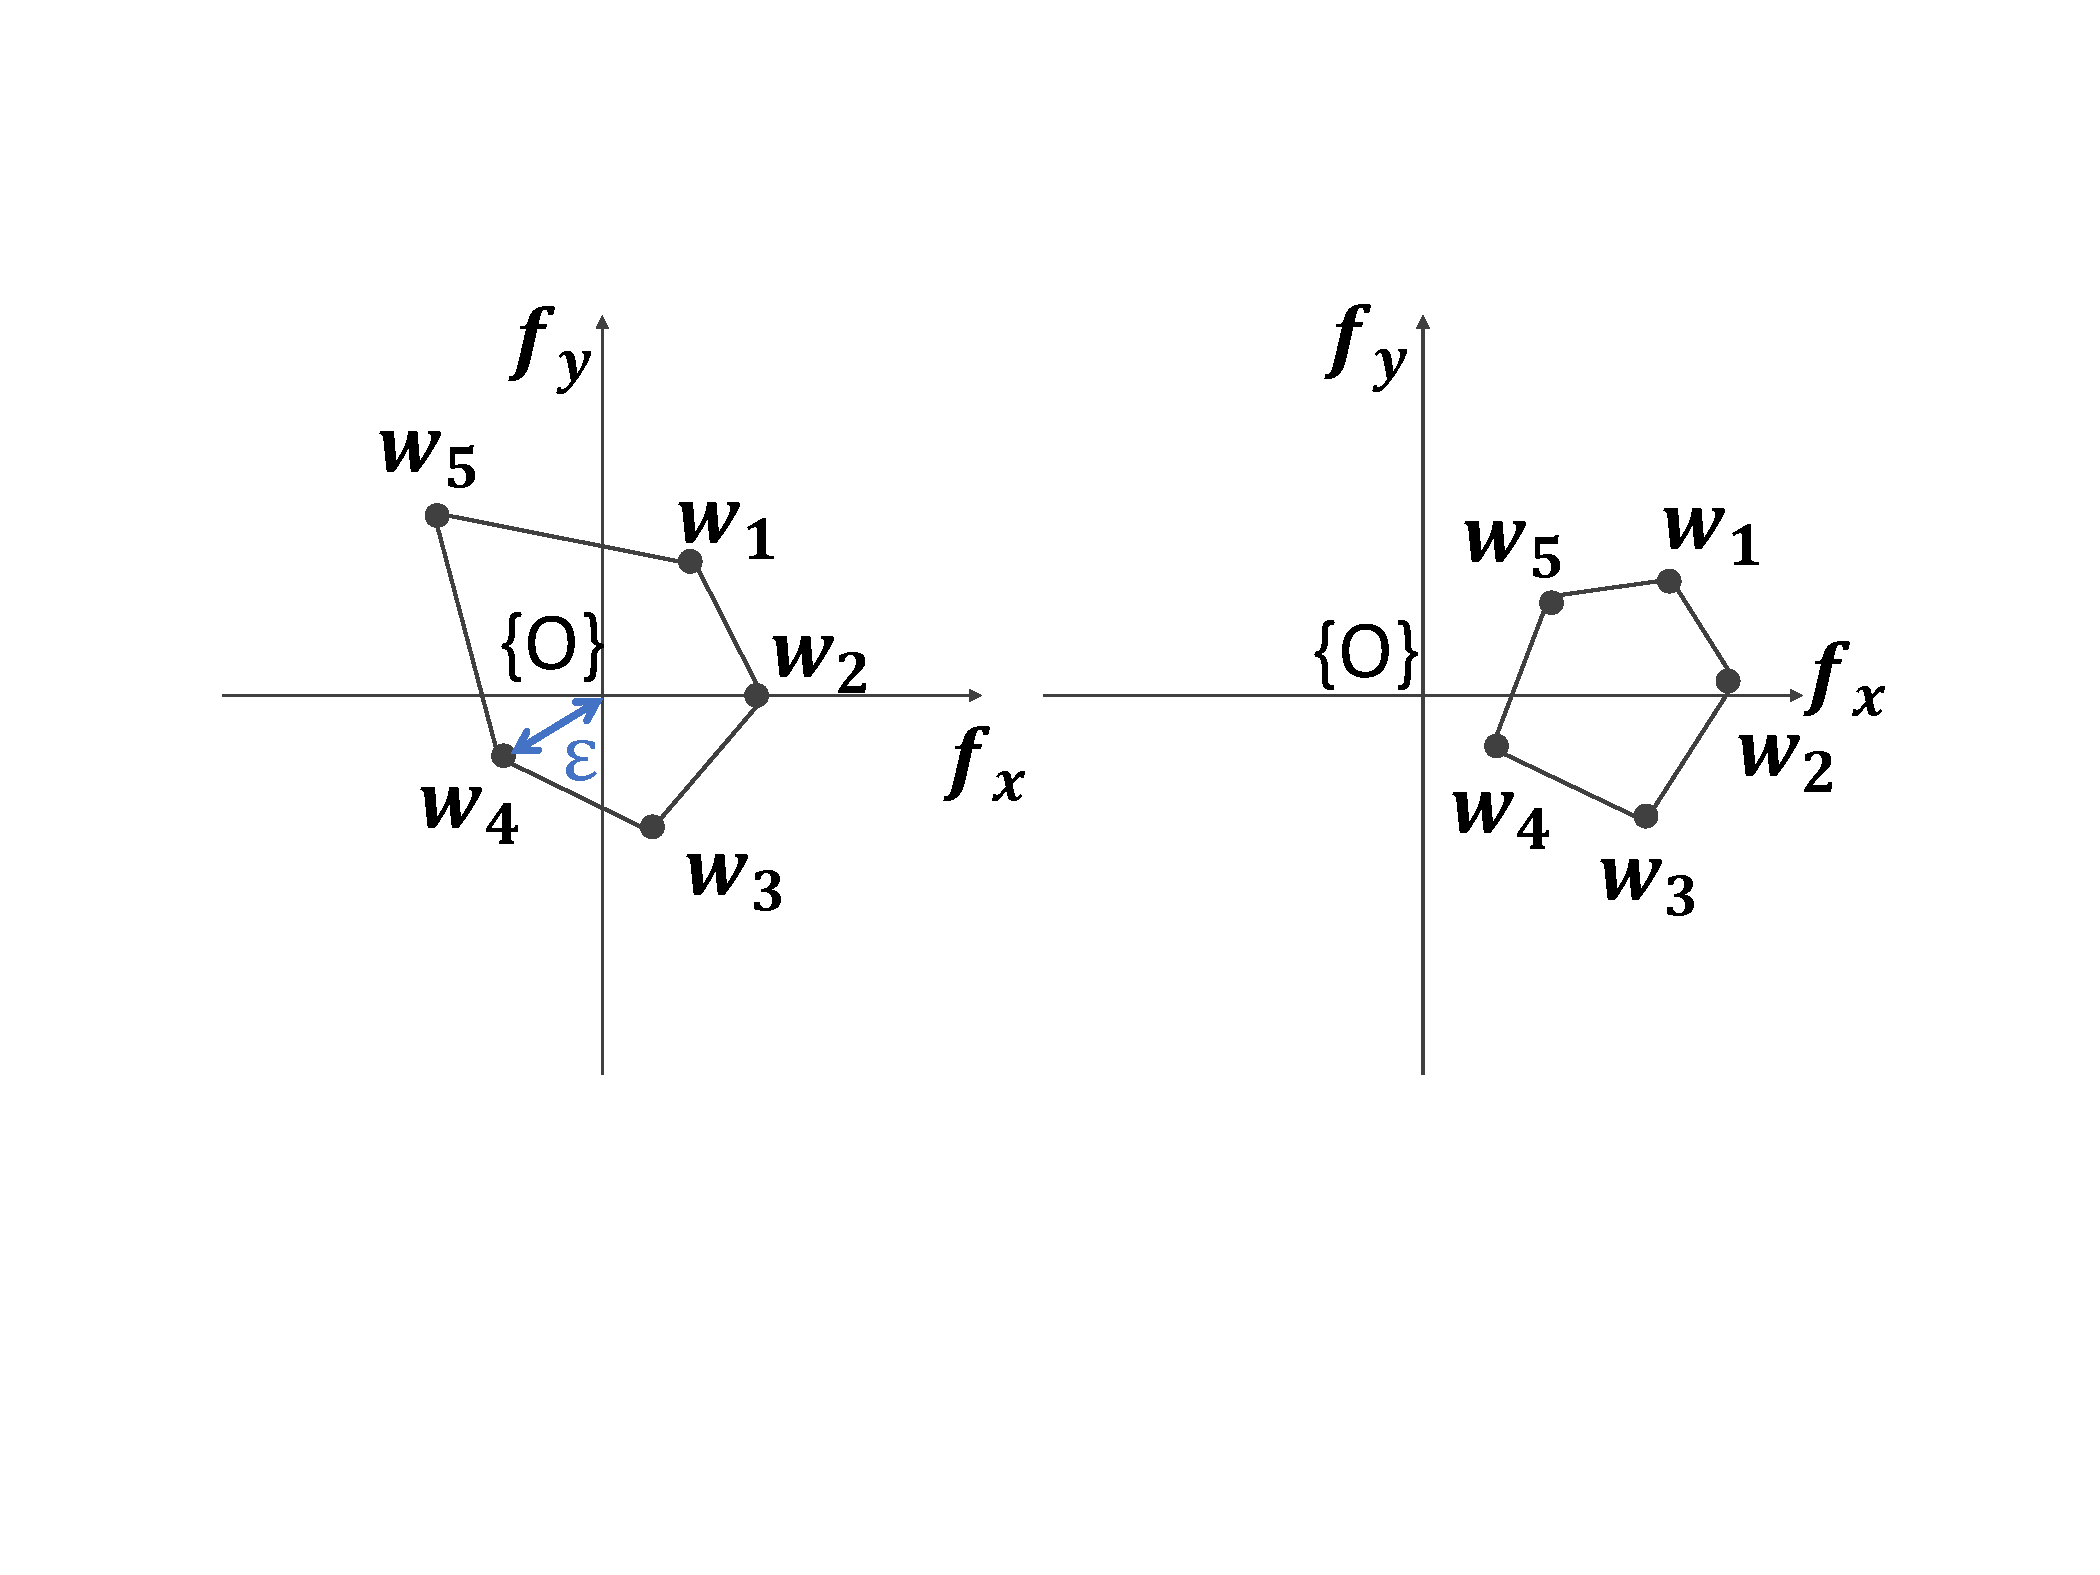
\includegraphics[trim={4cm 10cm 3cm 5cm},clip,width=1\linewidth,angle=0]{Cap2/Figuras/convex_hull_force_grasp.pdf}}
\centerline{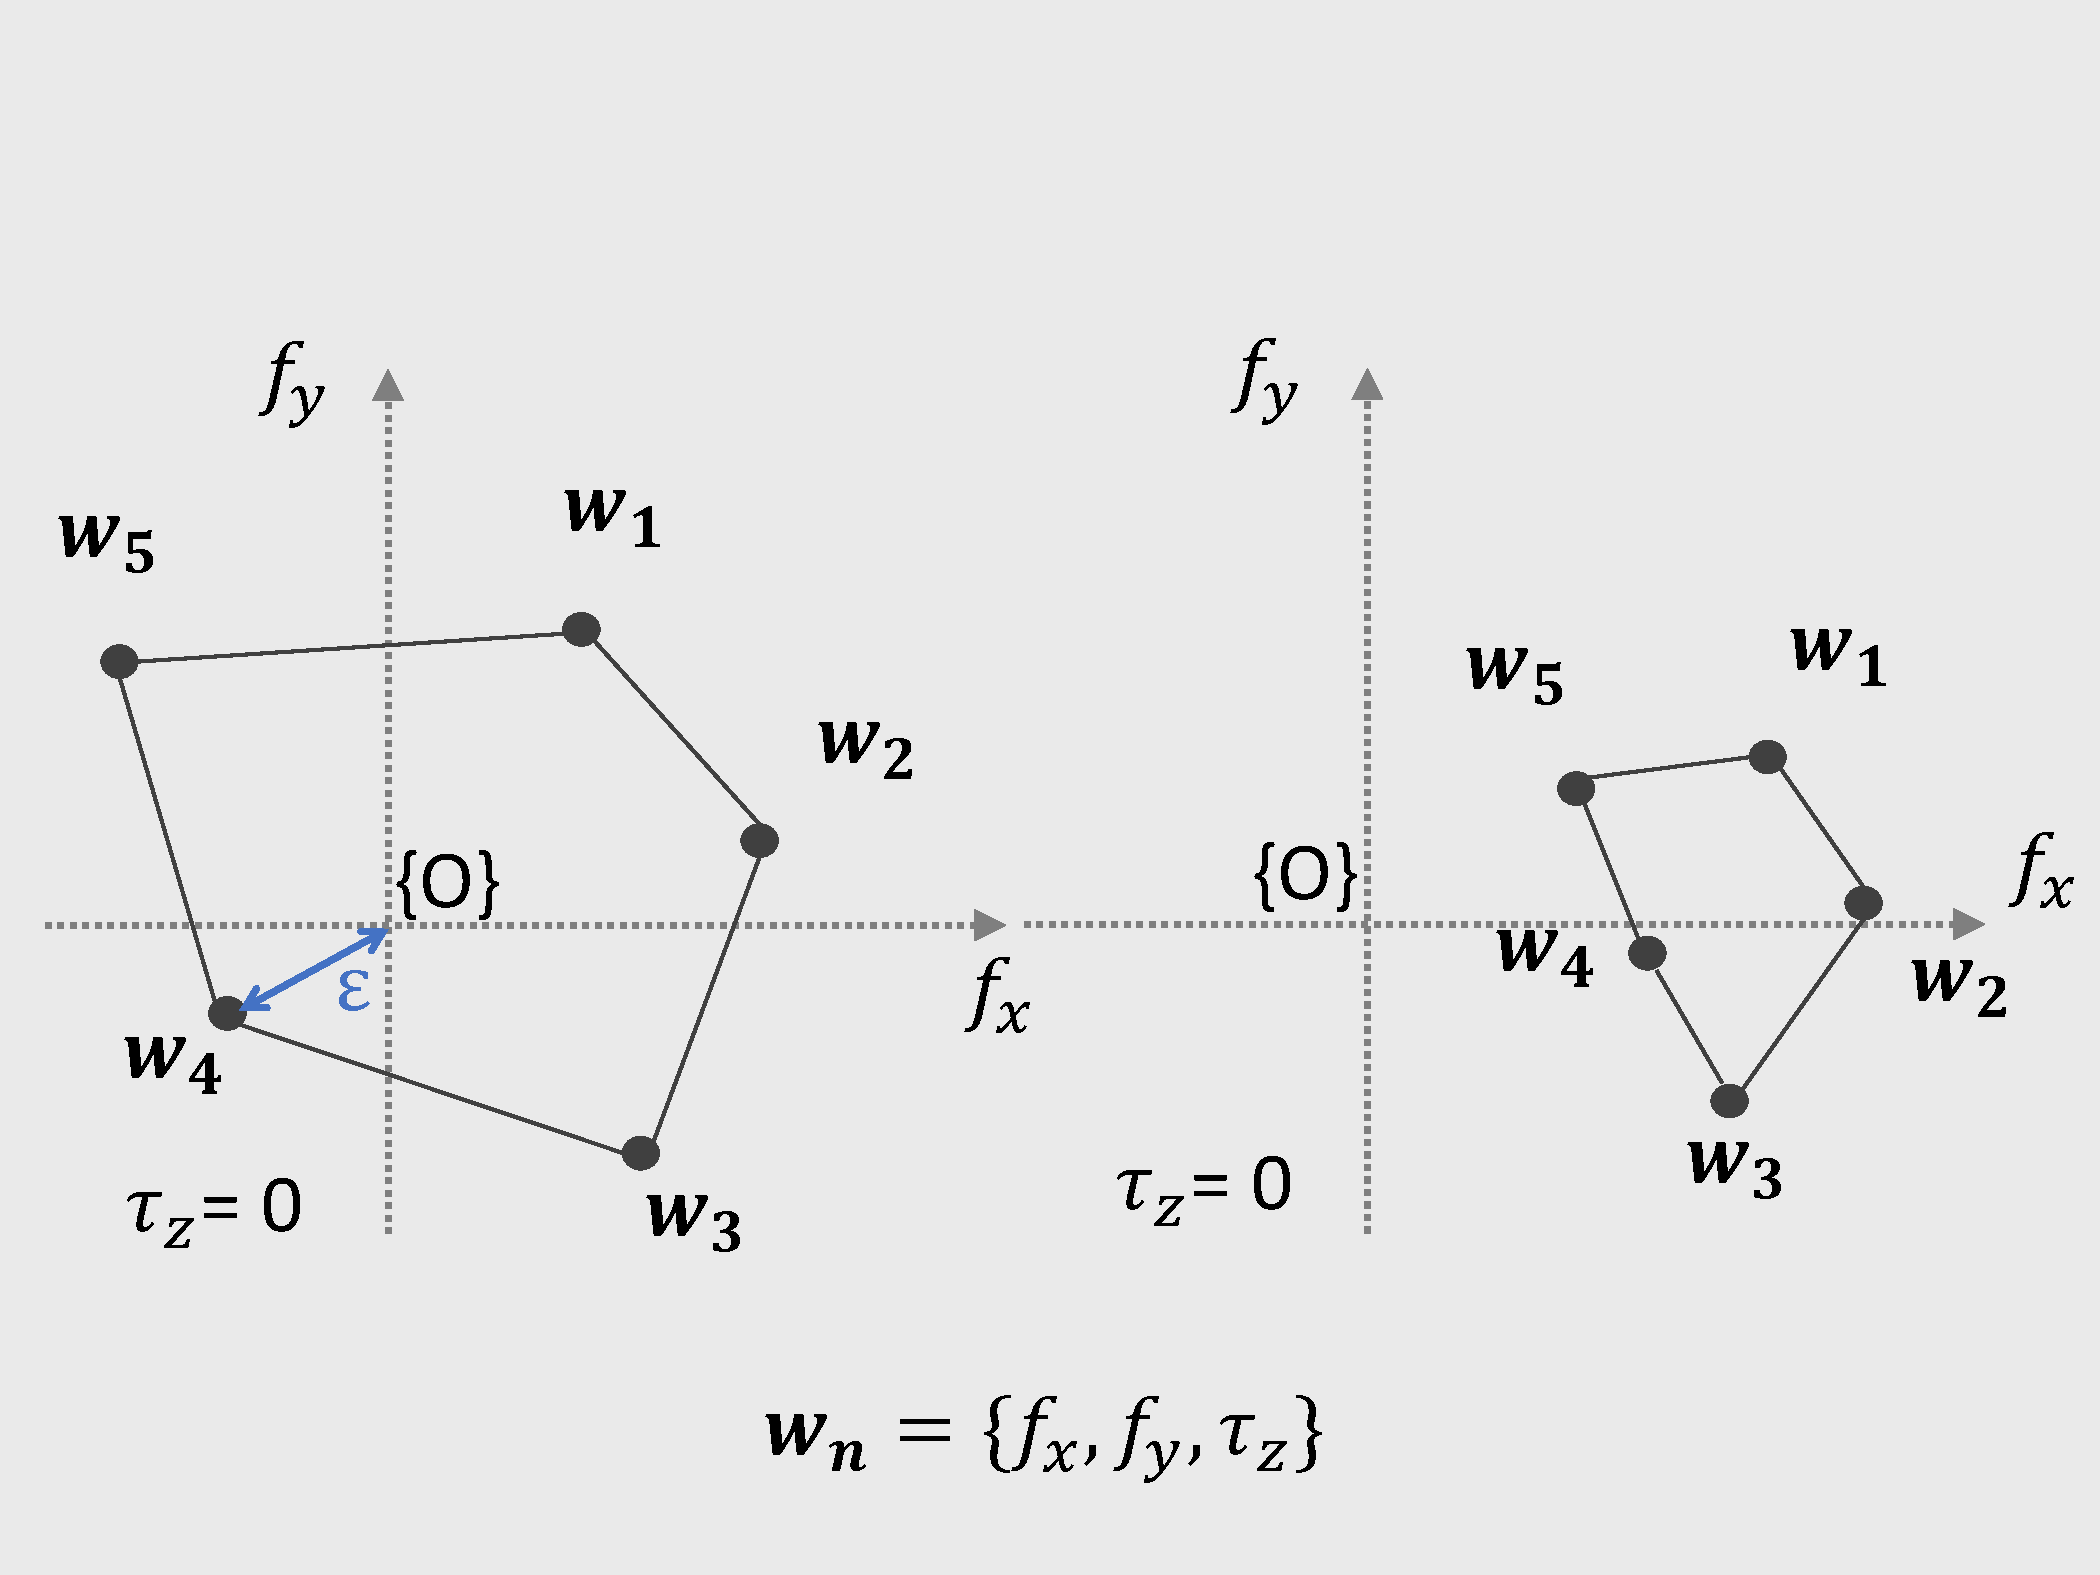
\includegraphics[trim={0cm 1.2cm 0cm 5.5cm},clip,width=0.65\linewidth,angle=0]{Cap2/Figuras/wrenchspace_anlayses_2.pdf}}
\captionof{figure}{Wrench space analyses representation}\label{fig:gws_force_closure_main}
\end{tcolorbox}

Following~\cite{Jiang2011a}, \citeauthor{Lenz2015}~\cite{Lenz2015} propose that the 6DOF-Rectangle could be simplified and confirm that this representation can be projected back to a 3DOF space. However, it was not explained this mapping. Later works~\cite{Redmon2015,Watson2017,Gariepy2019,asif2018ensemblenet} used this approach and achieved an interesting grasping detection success rate. 

\begin{tcolorbox}[every float=\centering, drop shadow, title= Antipodal Grasping]

 Two-finger contact with friction can be defined as force-closure if, and only if,  the line that connects each contact lays inside both friction cones. A non-force closure and a force closure antipodal grasping are represented by the left and right grasps of Figure~\ref{fig:antipodal}, respectively.

\vspace*{1ex}

\centerline{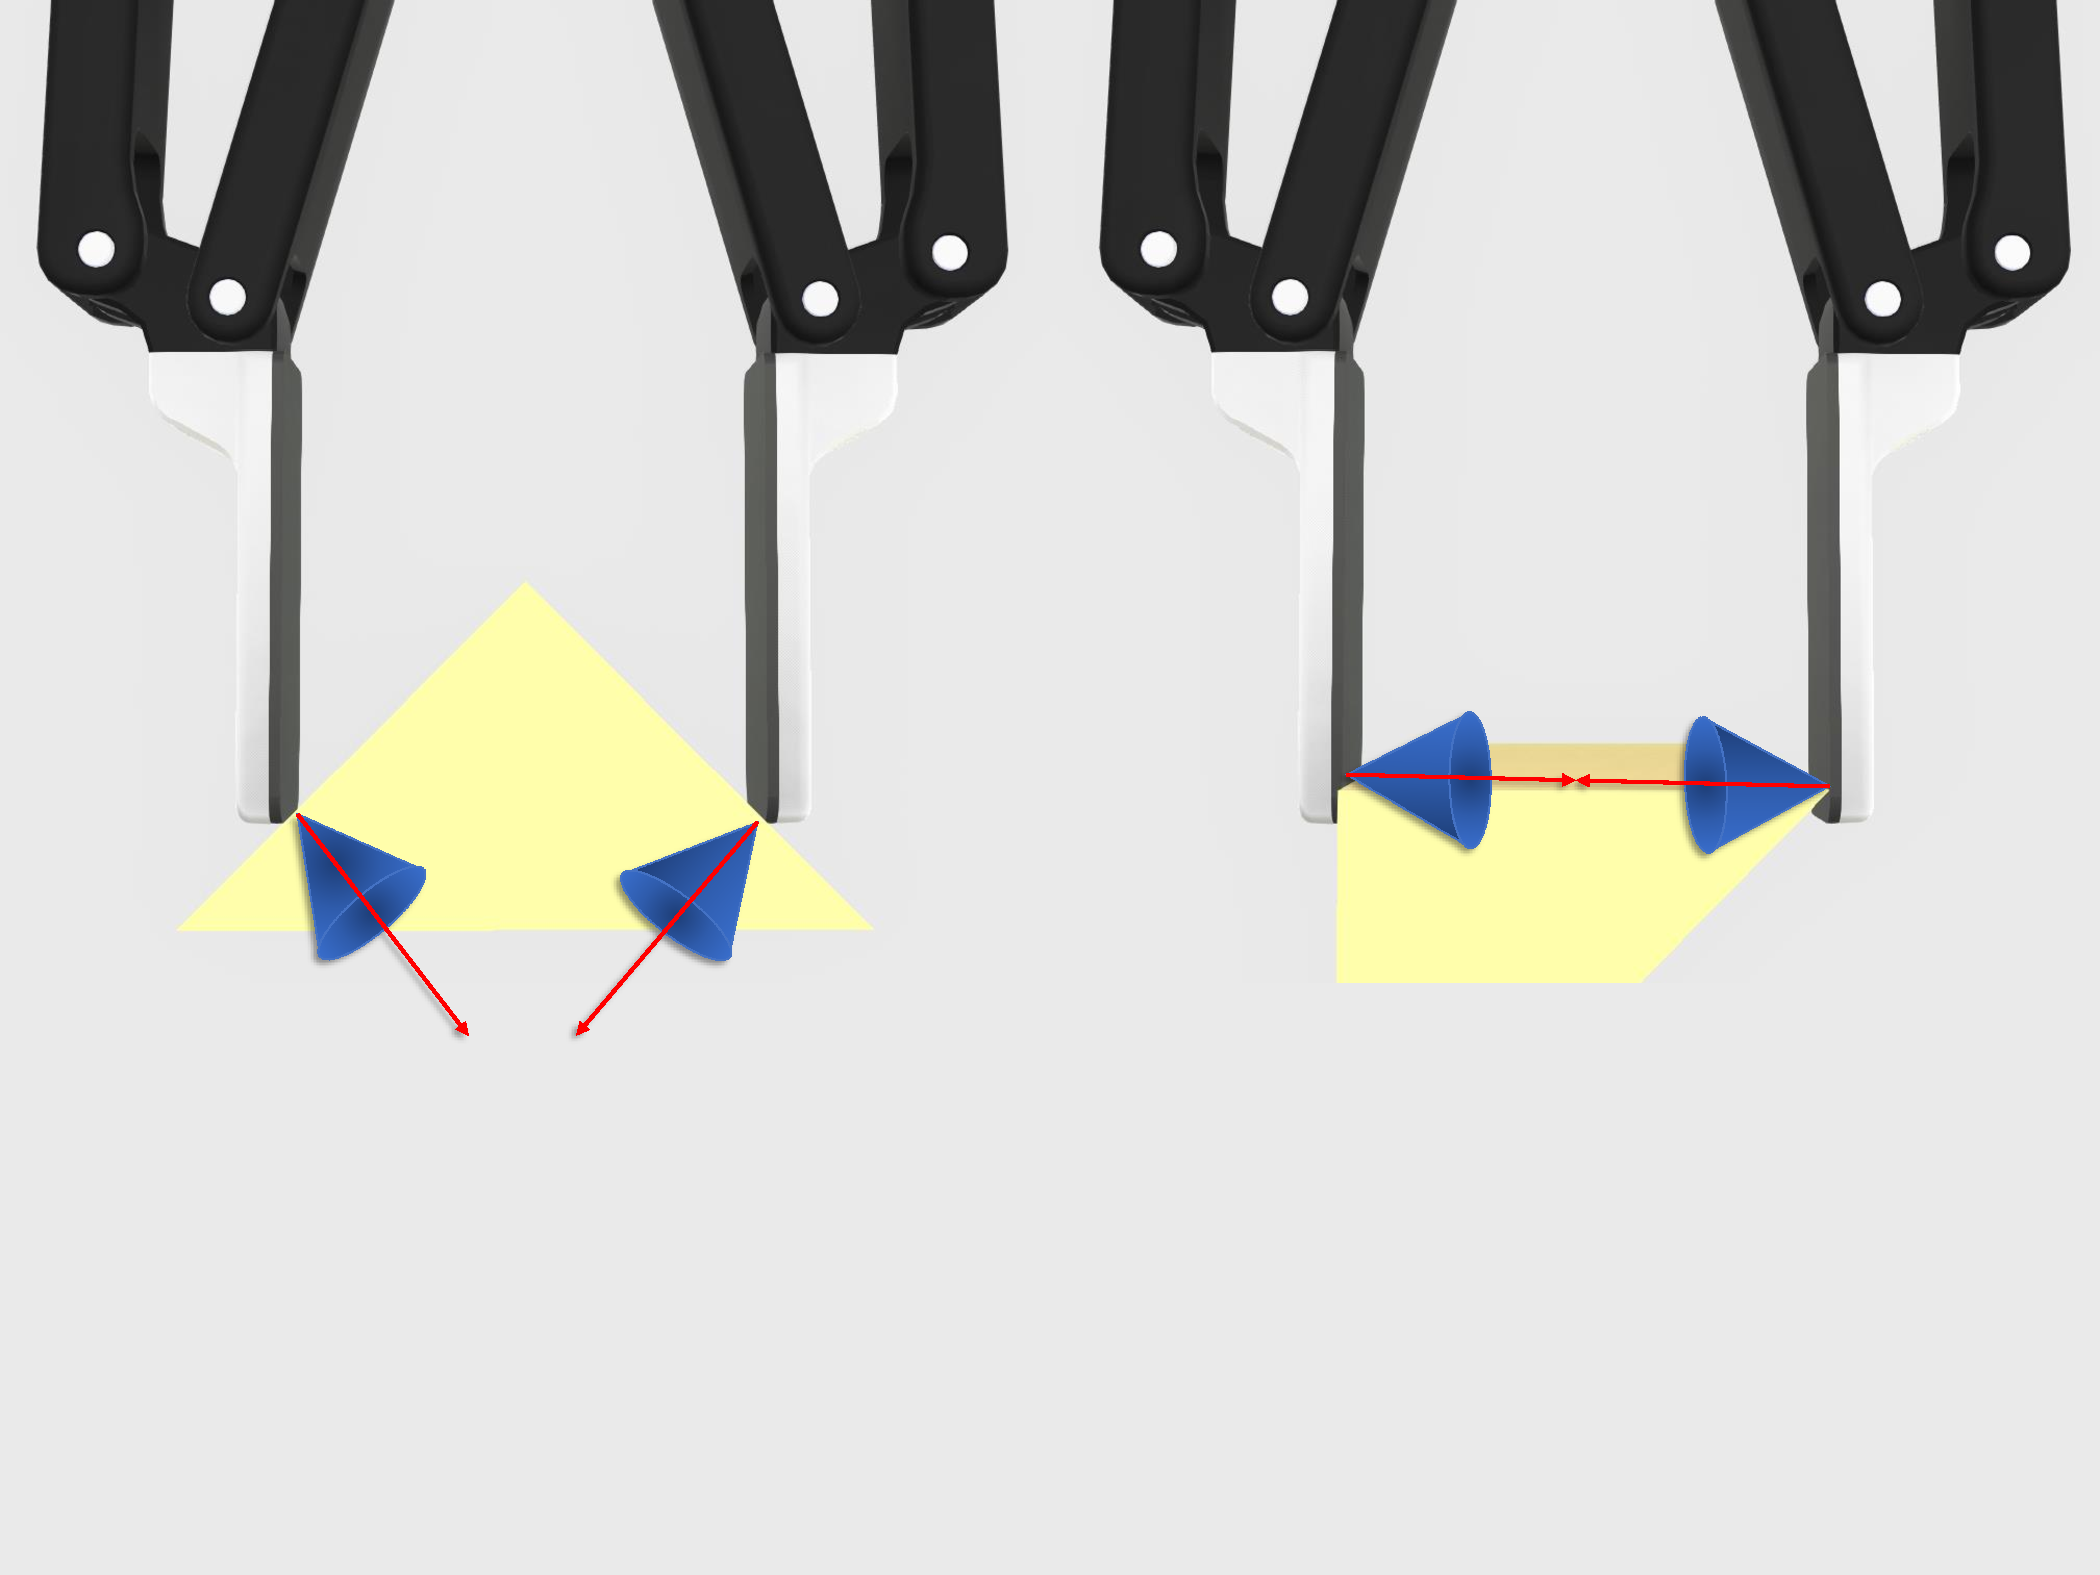
\includegraphics[trim={0cm 10cm 0cm 0cm},clip,width=.5\linewidth,angle=0]{Cap2/Figuras/antipodal_2.pdf}}
\captionof{figure}{Antipodal grasping restriction}\label{fig:antipodal}
\end{tcolorbox}


Even if several state-of-the-art works use these image-based metrics to assess the efficiency of grasping detection, this approach is questionable ~\cite{Guo2017,Gariepy2019,Mousavian_2019_ICCV,Ghazaei2019,TenPas2017,choi2018learning, Chen2019}. Some authors~\cite{Gariepy2019,Ghazaei2019} affirm that the grasping is not completely defined like an object's classification in an image, i.e., there still exist many grasping possibilities which are not mapped in a ground-truth database. Despite the gripper's physical limitations of rectangle representation modelling,  it is possible to note that the grasping performance does not reflect several works' success detection rates. This approach does not consider the real physical interactions between active pairs, e.g., force-closure properties and Coulomb's law. It also does not consider sensing noises and robot action's inconsistencies. Thus, \citeauthor{Guo2017}~\cite{Guo2017} propose a hybrid deep learning architecture combining the visual rectangle representation and tactile sensing for robotic grasping detection. Their experiments indicate that tactile data improve the grasping detection task. \citeauthor{Ghazaei2019}~\cite{Ghazaei2019} present the grasping belief maps to generate a set of grasping over an image without classifying the object whilst considering uncertainties (Figure~\ref{fig:exemples_rep}). A similar approach of pixel-wise representation is also verified by~\cite{Zeng2018}. Another continuous approach is the Grasp Path proposed by~\cite{Chen2019,Chen2020} (see Figure~\ref{fig:exemples_rep}). Asserting that the predicted comparison with the ground-truth database could eliminate other graspable candidates that are not included in the overlap threshold, the authors of~\cite{Chen2019,Chen2020} formulated a path that leads to the set configuration of rectangular grasping poses. In their tests, Grasp Path show to be less dependent on the Jacquard threshold. 


\begin{figure}[h!]
	\resizebox{.75\textwidth}{!}{%
		\begin{tcolorbox}
			\centering
			\begin{subfigure}[c]{0.45\textwidth}
				\centering
				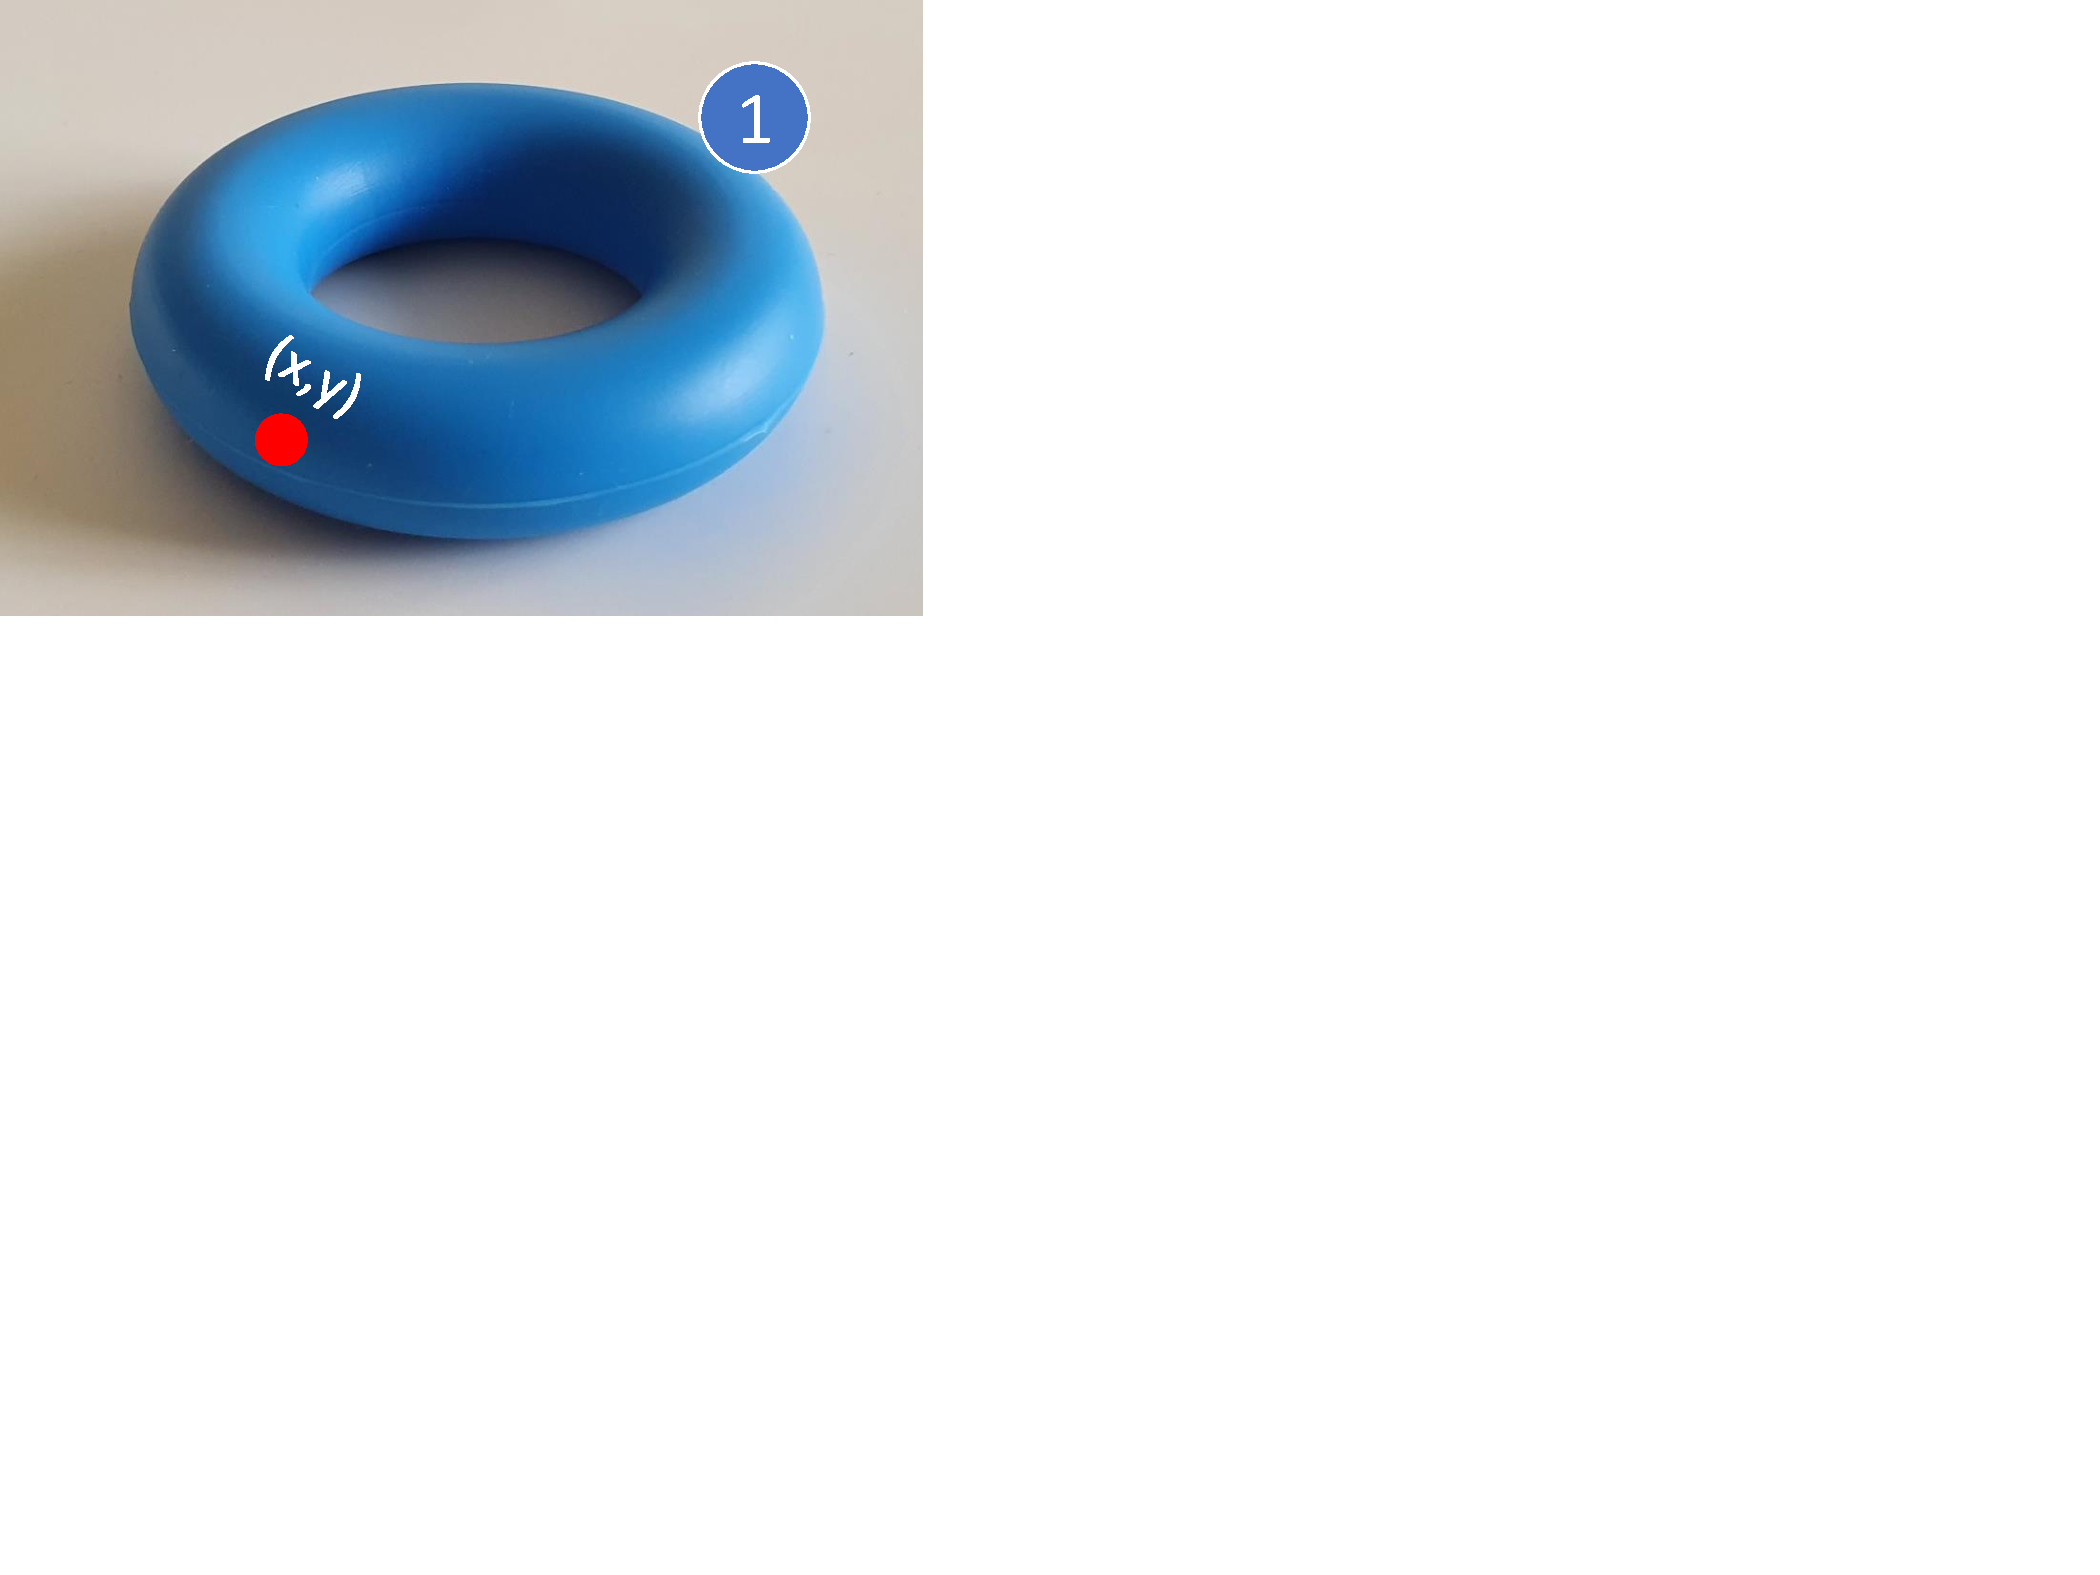
\includegraphics[trim={19mm 162mm 215mm 8mm},clip,width=1\columnwidth,angle=0]{Cap2/Figuras/point_rep.pdf}
				%\caption{Pure enclosing without clamping.}
				%\label{fig:g1}
			\end{subfigure}
			\hfill
			\begin{subfigure}[c]{0.45\textwidth}
				\centering
				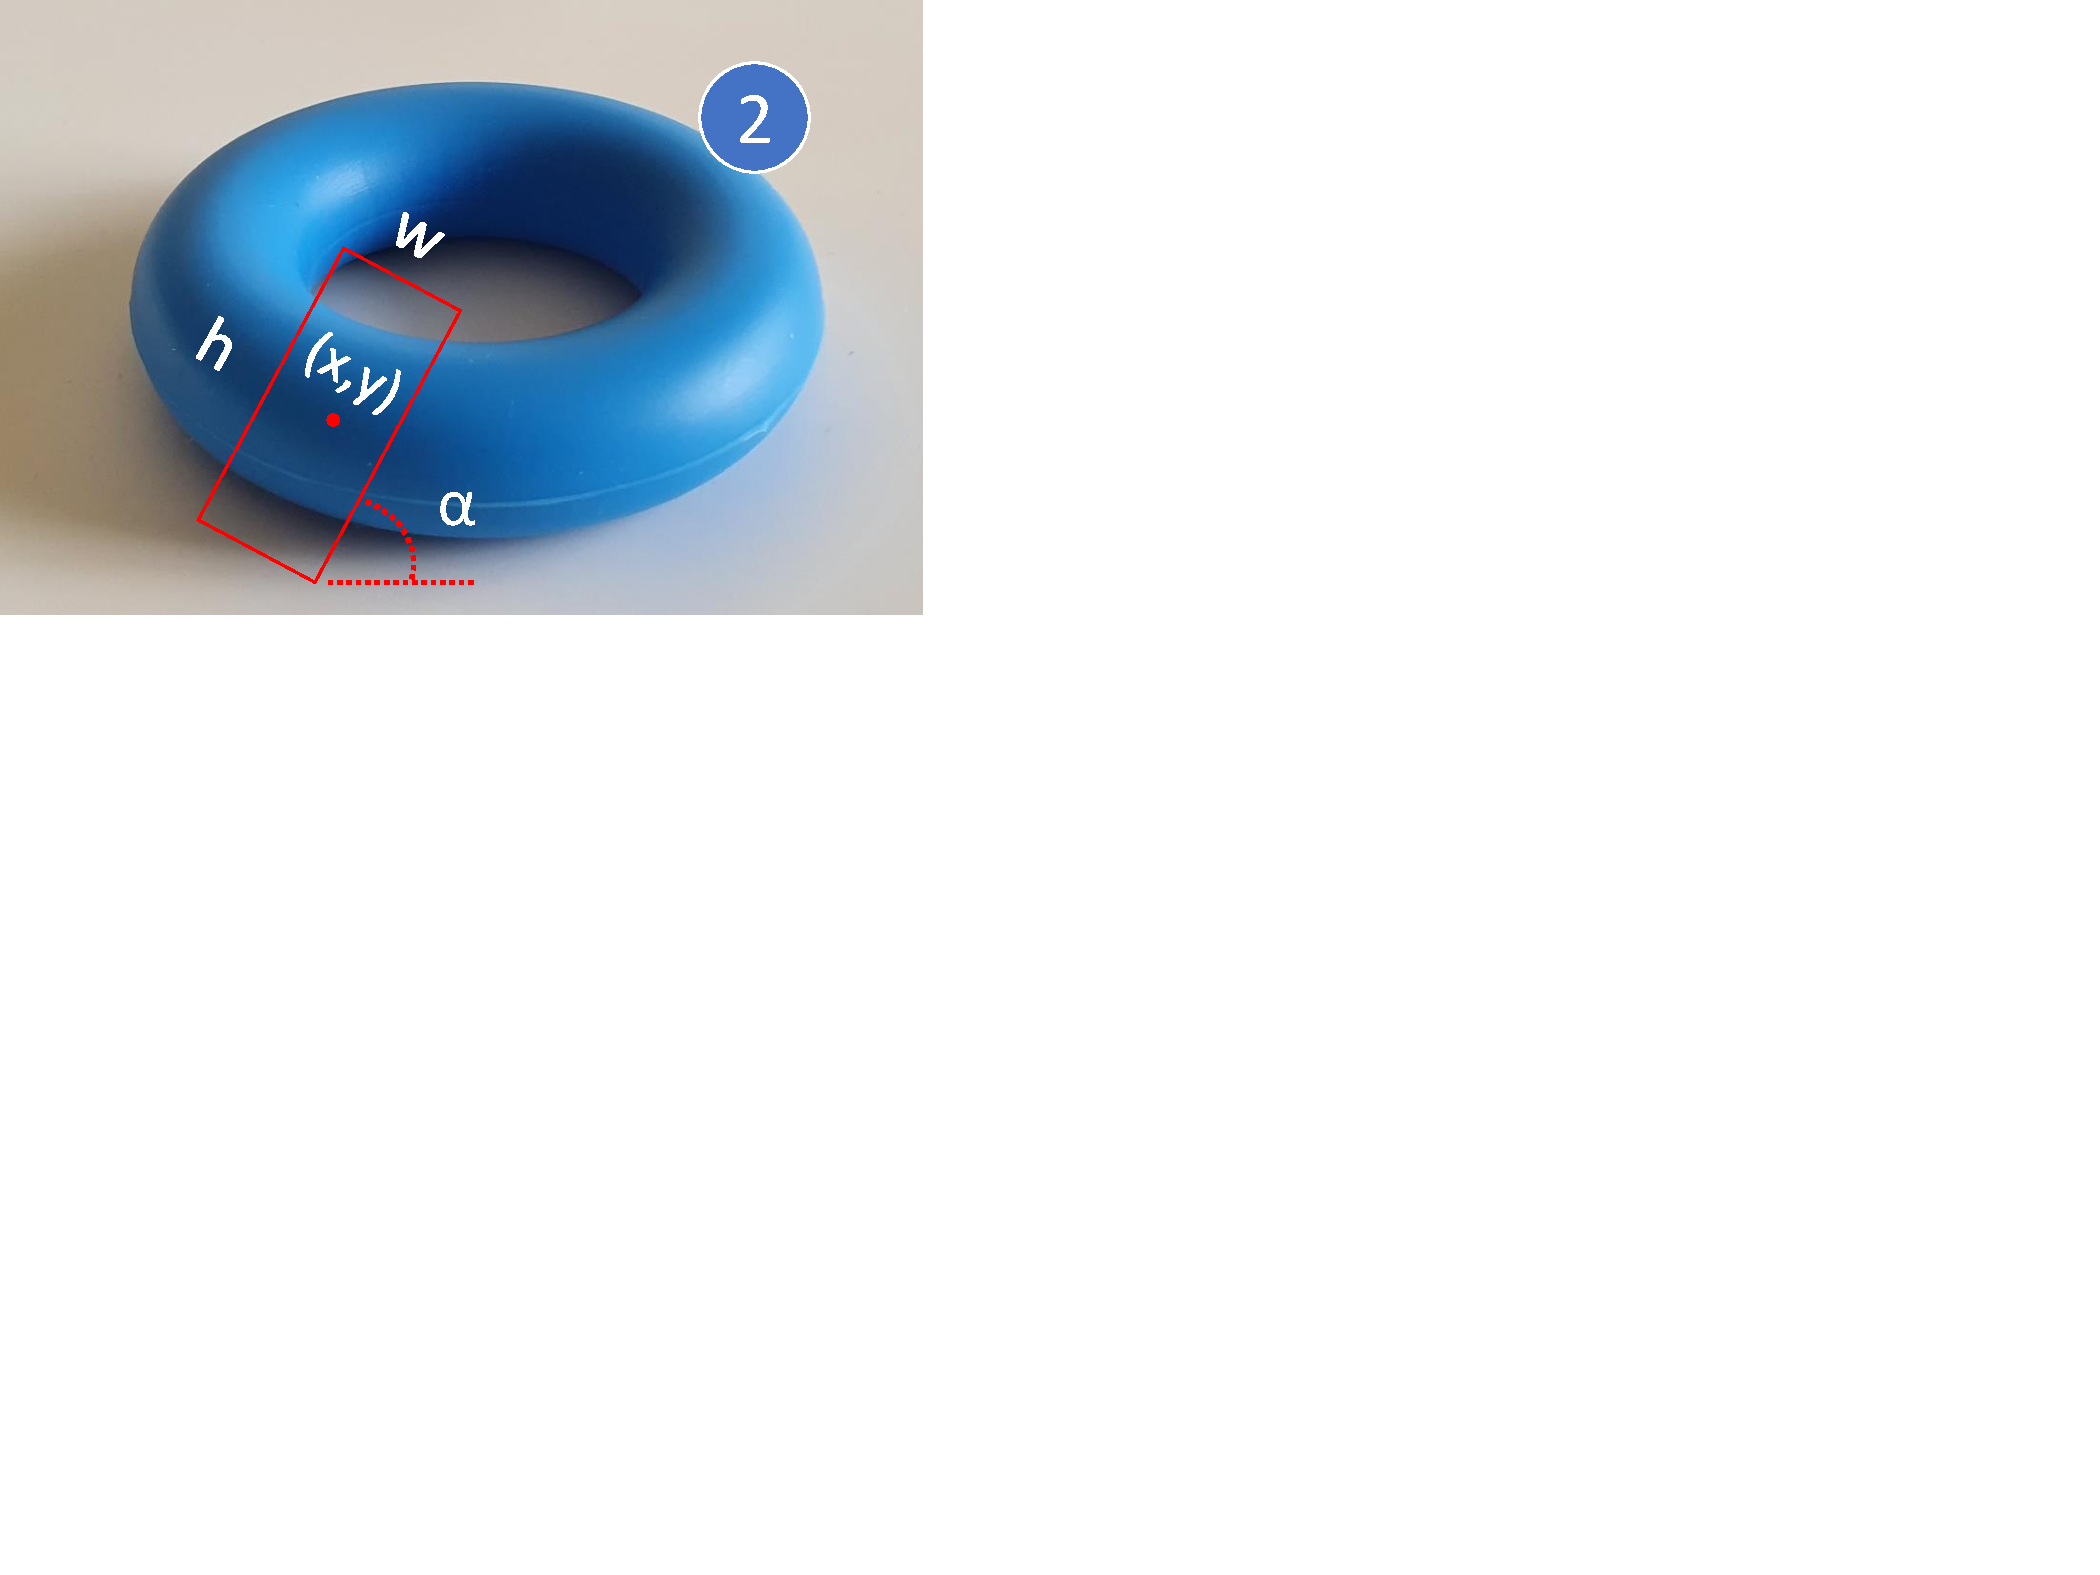
\includegraphics[trim={19mm 162mm 215mm 8mm},clip,width=1\linewidth,angle=0]{Cap2/Figuras/rec_rep.pdf}
				%\caption{Partial form fit combined with clamping force.}
				%\label{fig:g2}
			\end{subfigure}
			\hfill
			\begin{subfigure}[c]{0.45\textwidth}
				\centering
				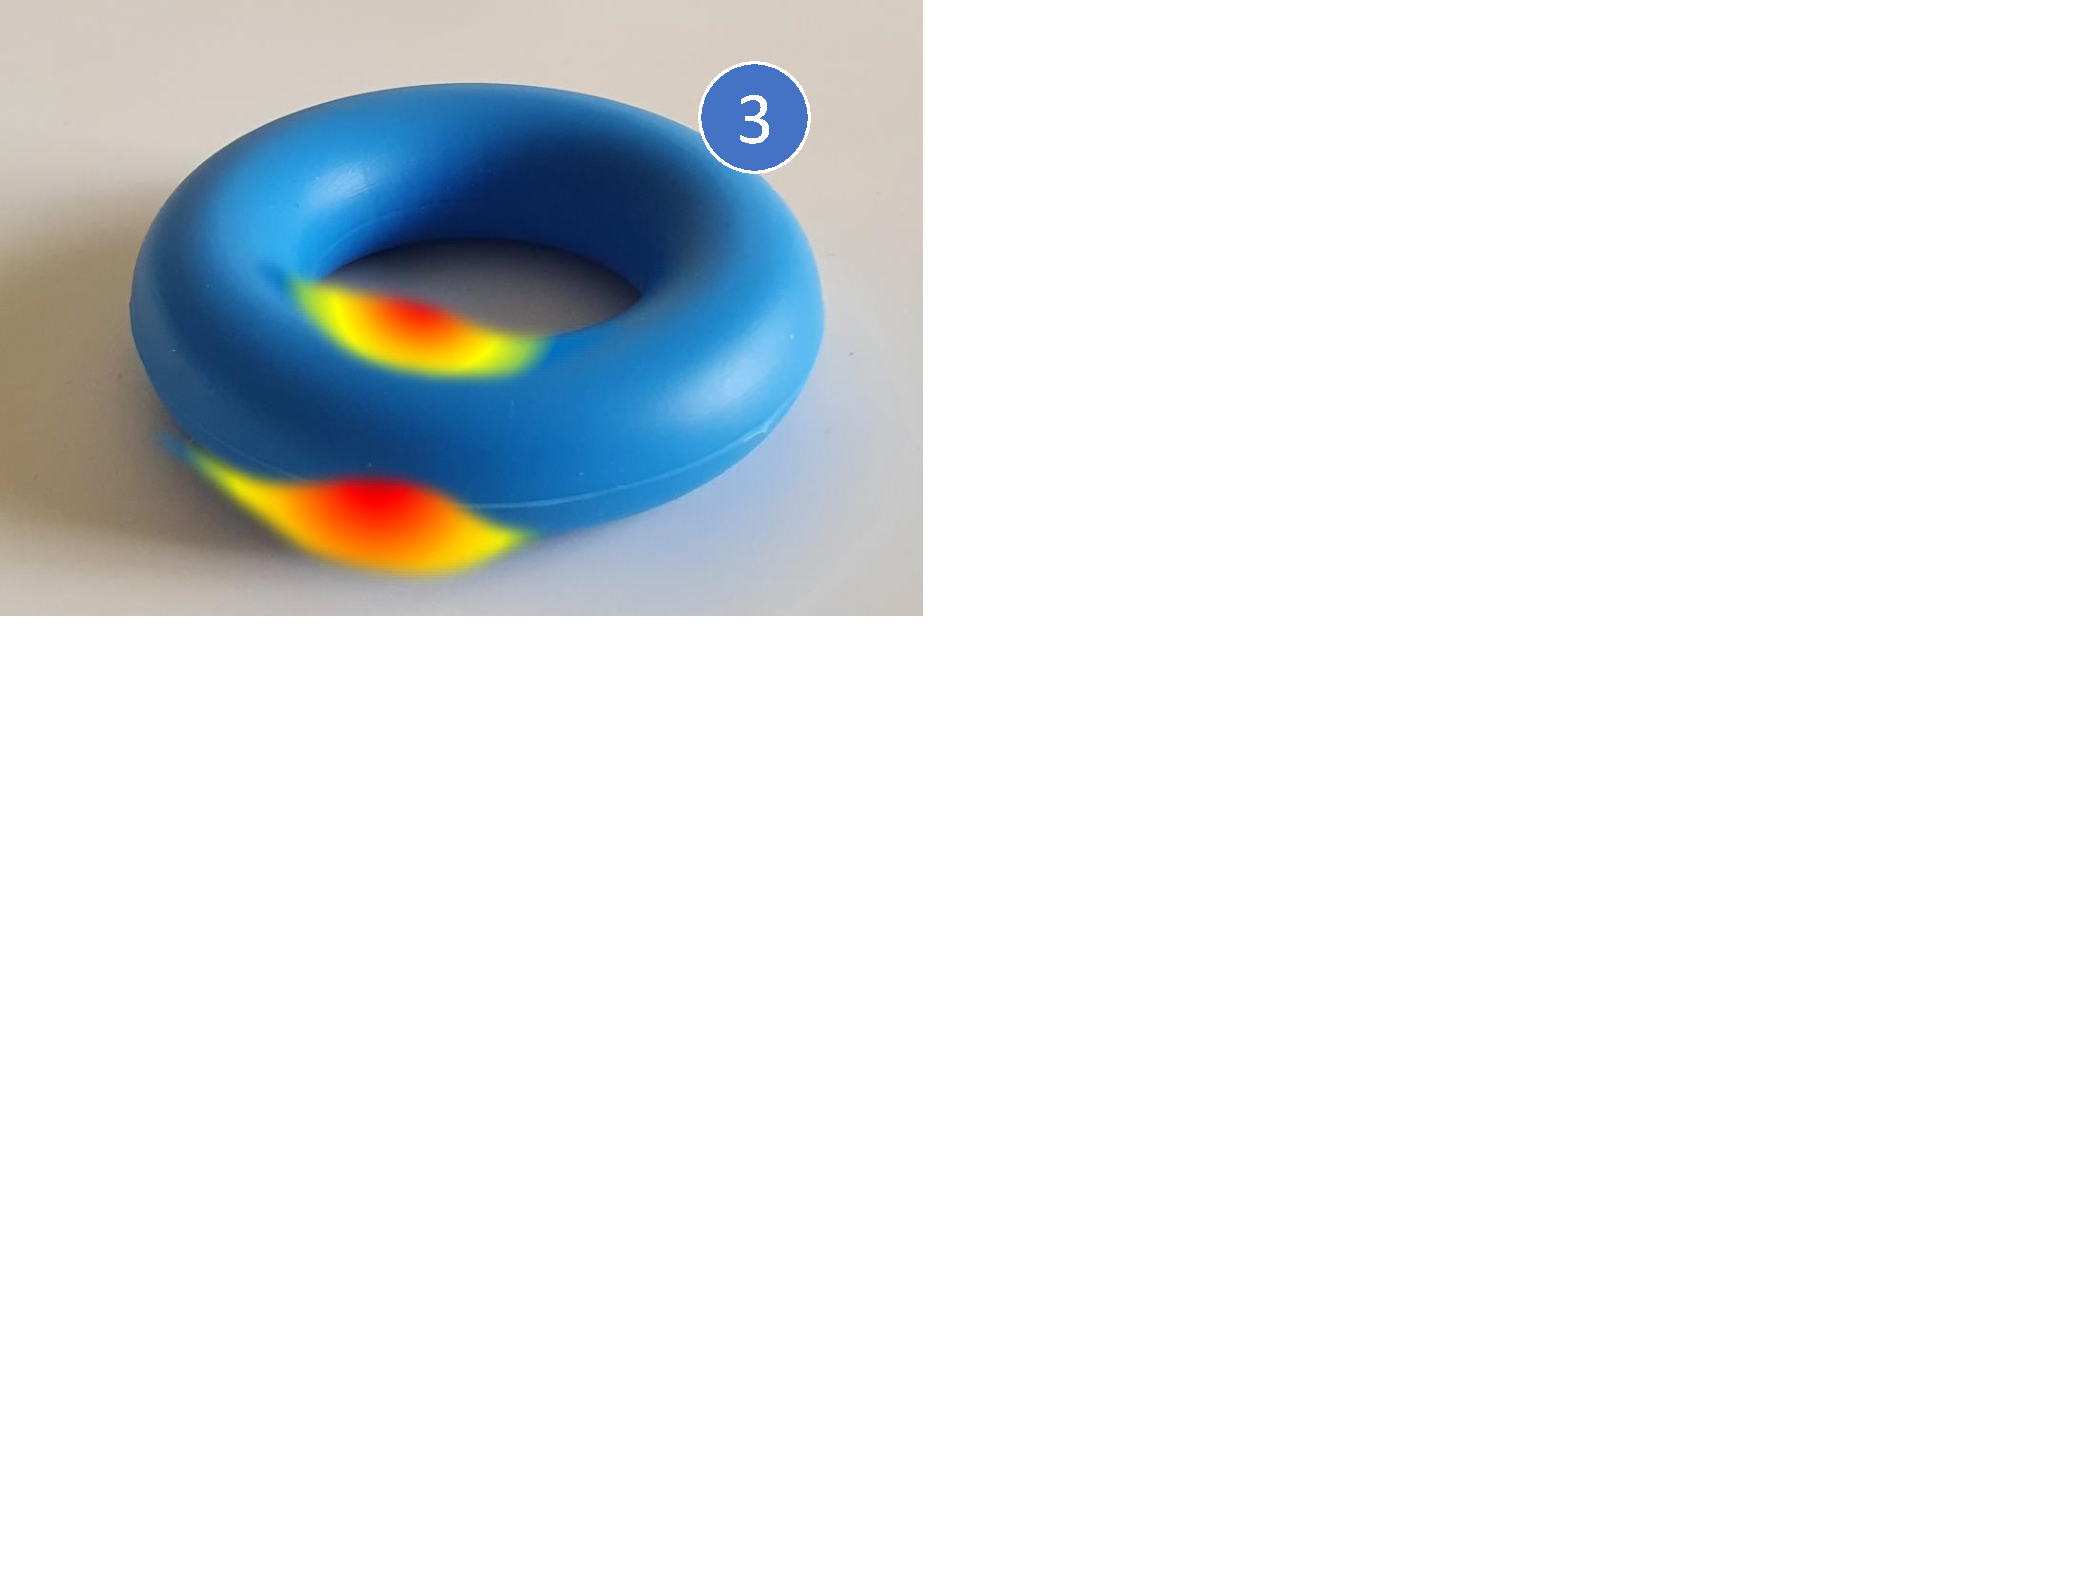
\includegraphics[trim={19mm 162mm 215mm 8mm},clip,width=1\columnwidth,angle=0]{Cap2/Figuras/myBeliefMap.pdf}
				%\caption{Pure force closure.}
				%\label{fig:g3}
			\end{subfigure}
			\hfill
			\begin{subfigure}[c]{0.45\textwidth}
				\centering
				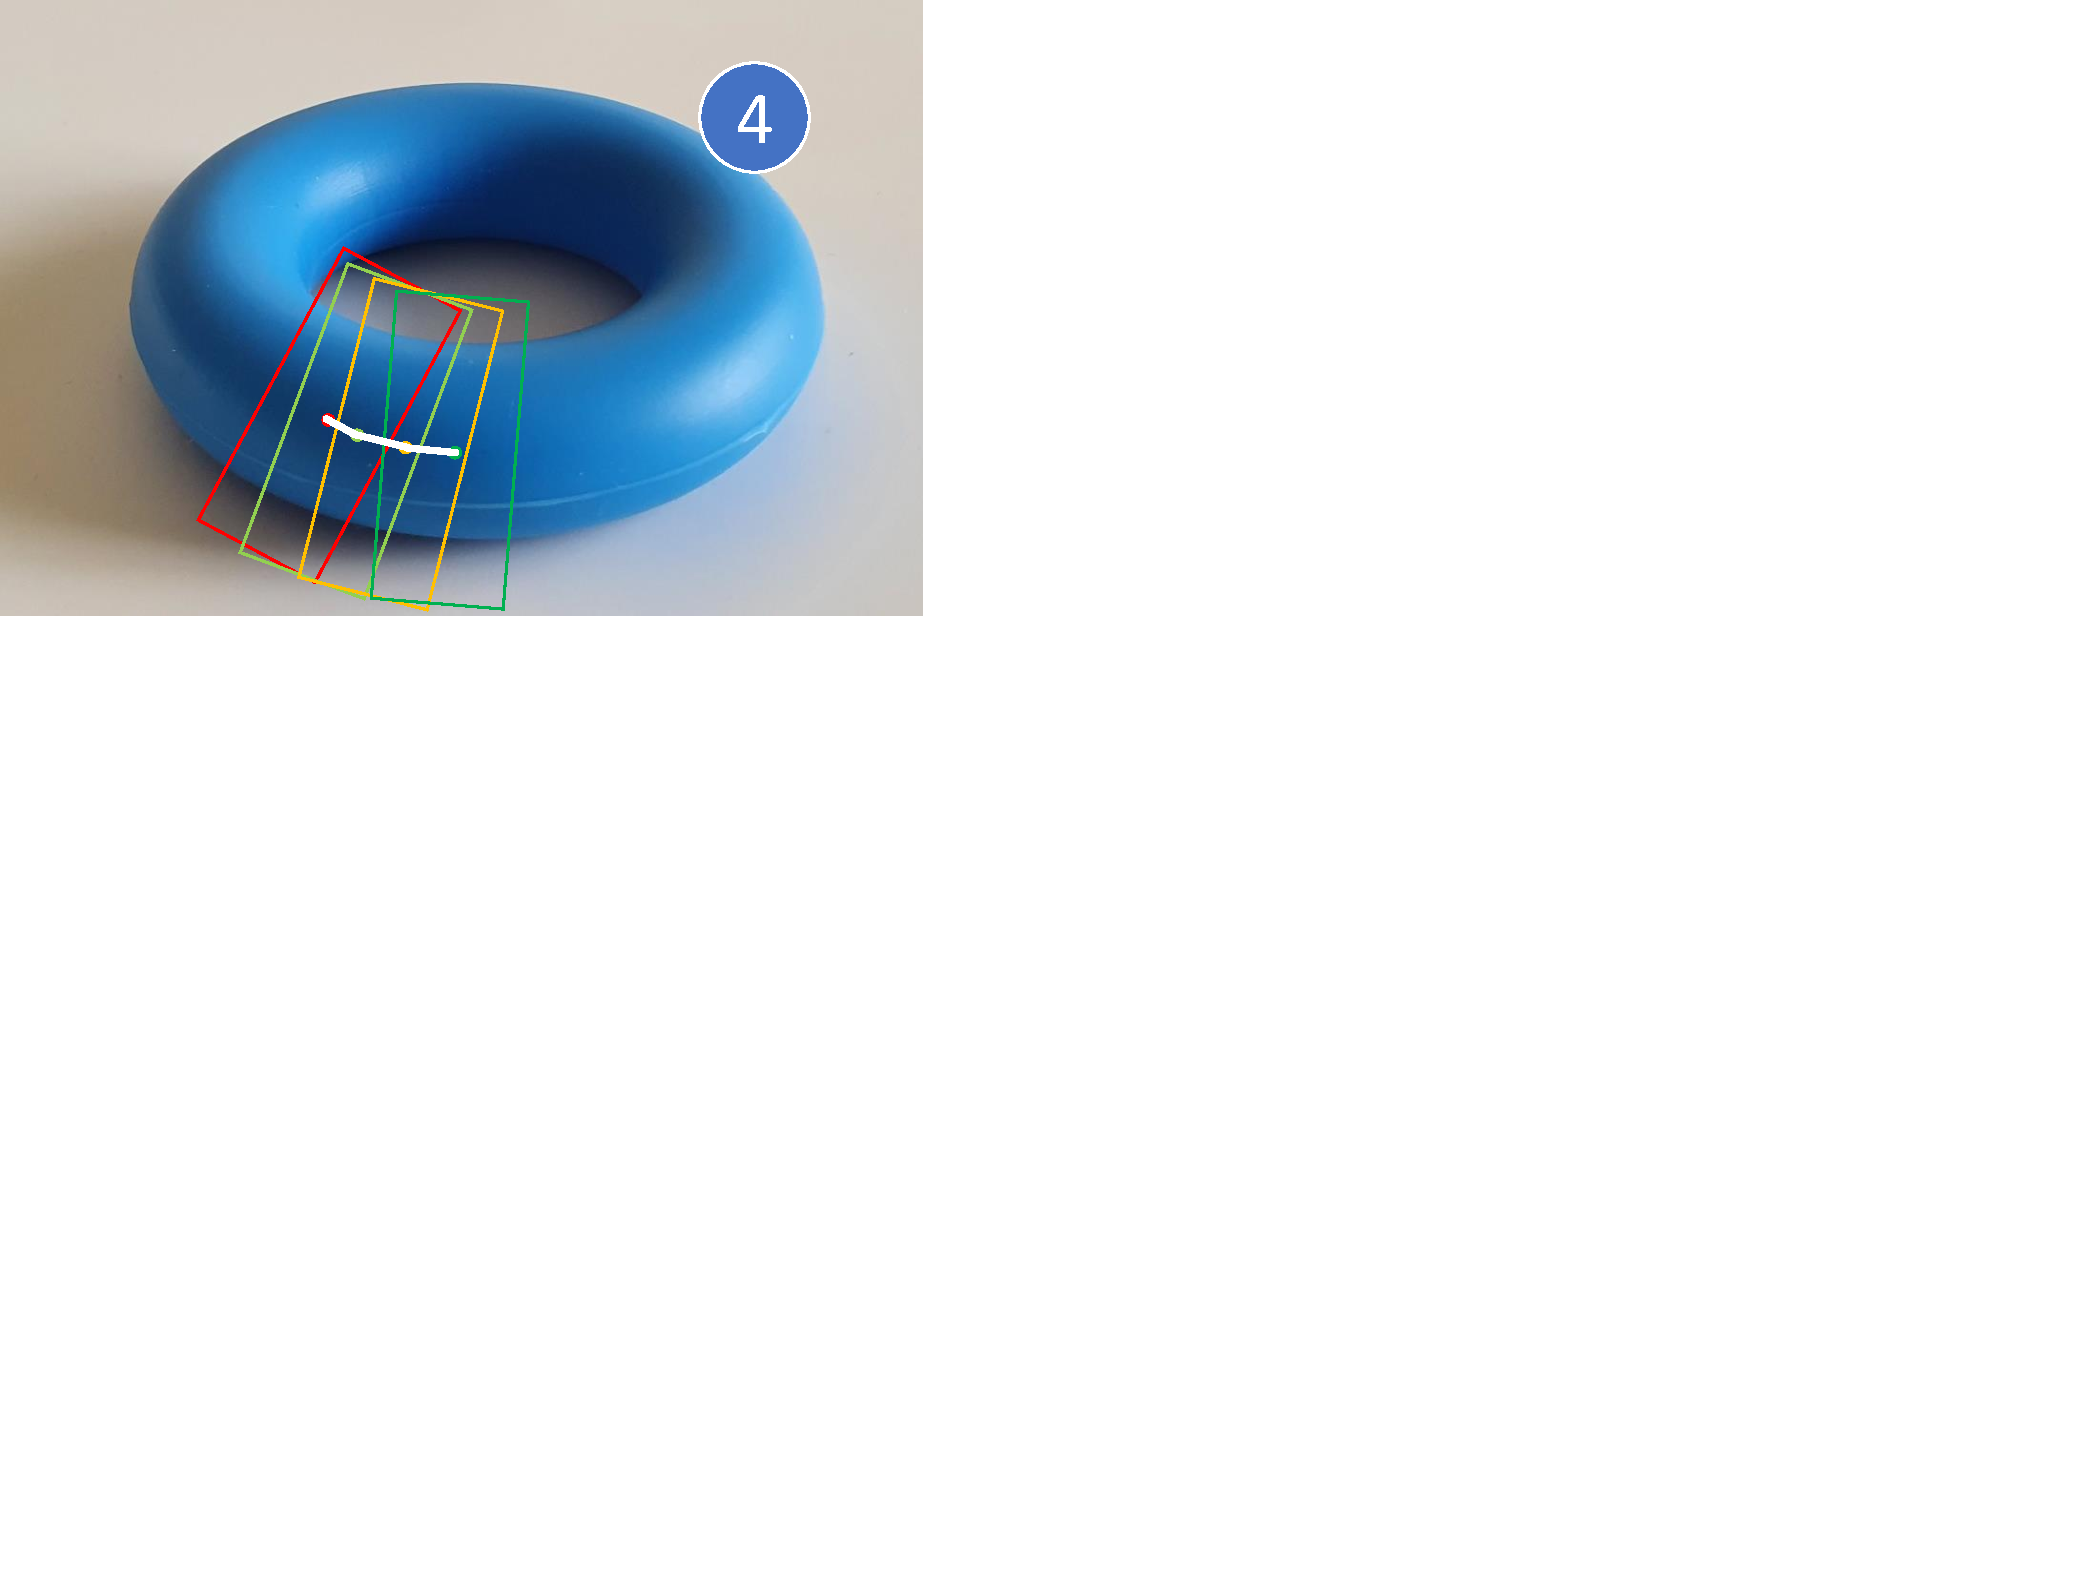
\includegraphics[trim={19mm 162mm 215mm 8mm},clip,width=1\linewidth,angle=0]{Cap2/Figuras/myGraspPath.pdf}
				%\caption{Holding with vacuum air (pneumatic force closure).}
				%\label{fig:g4}
			\end{subfigure}
		\end{tcolorbox}
		\caption{Grasping representation in 2D images. Grasping point (1) describes a grasping position $(x,y)$ without any physical considerations, while the rectangle representation (2) also represents the gripper's width ($w$), height ($h$), and orientation ($\alpha$). The grasping belief map (3) models a spatial uncertainty in a grasp distribution fashion. The grasping path (4), described by a white line, leads the prediction of several possible rectangle grasp candidates.}
		\label{fig:exemples_rep}
	}%end of resize box      
\end{figure}



%\begin{figure}[h]
%    \centering
%    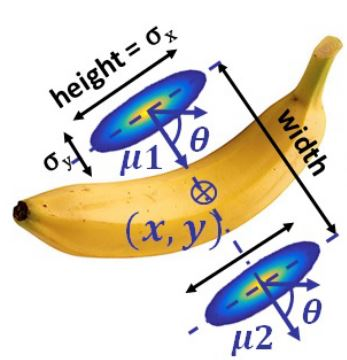
\includegraphics[scale=0.5]{Cap2/Figuras/grasping_belief_map.JPG} 
%    \caption{Grasping Belief Maps and Grasp Path.}
%    \label{fig:grasp_belief_grasp_path}
%\end{figure}

% \begin{figure}[h]
%     \centering
%     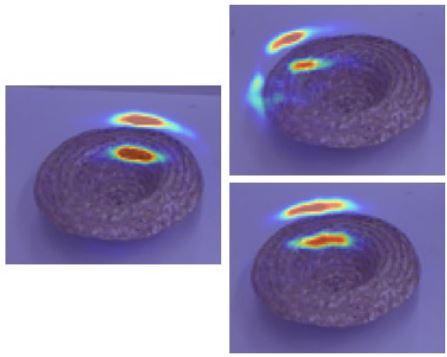
\includegraphics[scale=0.75]{Cap2/Figuras/grasping_belief_map2.JPG} 
%     \caption{Grasping Belief Maps~\cite{Ghazaei2019}.}
%     \label{fig:grasp_belief_map}
% \end{figure}

% \begin{figure}[h]
%     \centering
%     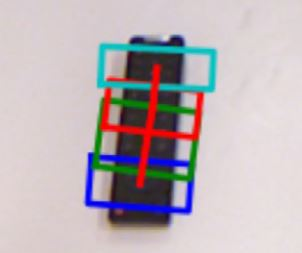
\includegraphics[scale=.5]{Cap2/Figuras/grasp_path.JPG} 
%     \caption{Grasp Path~\cite{Chen2019}}
%     \label{fig:grasp_path}
% \end{figure}

%\subsection{Discussion}
%\label{cap2:related_work:sec:grasping_representation:subsec:discussion}


As it is possible to see in this section, grasping representation is an essential phase in grasping planning. The mathematical formulation and description, such as wrench space analyses, antipodal restriction, $\epsilon$, and volume metrics are the basis for understanding physical phenomena between the active-pair interaction, e.g., basis widely used in 3D model grasping representations (3D-sensing and CAD simulations). However, these mathematical description techniques showed to be limited by several factors, e.g., high complexity implementation according to application demands and the necessity to know the gripper and graspable object characteristics. Therefore, these approaches typically work well only in specific cases.  

\begin{tcolorbox}[every float=\centering, drop shadow, title= Jacquard threshold]
	
	The Jacquard threshold also referred to as the Jacquard index, is commonly used as a quality metric for grasping predictions. The mathematical formulation is defined by $Area(G\cap G^*)/Area(G\cup G^*)$, where $G$ and $G^*$ are the predicted and the ground-truth grasping rectangles, respectively. It is restricted to rectangle grasping representation which is widely used by two-finger grasps. It is important to notice that this approach can lead to miss concept conclusions since the high Jacquard index is not completely related to grasping success, e.g different rectangle orientations can have the same intersection region, therefore the same Jacquard value, and lead to unfeasible grasps. Thus, it is common that this metric has complementary analyses in several works.
	
	\vspace*{1ex}
	
	\centerline{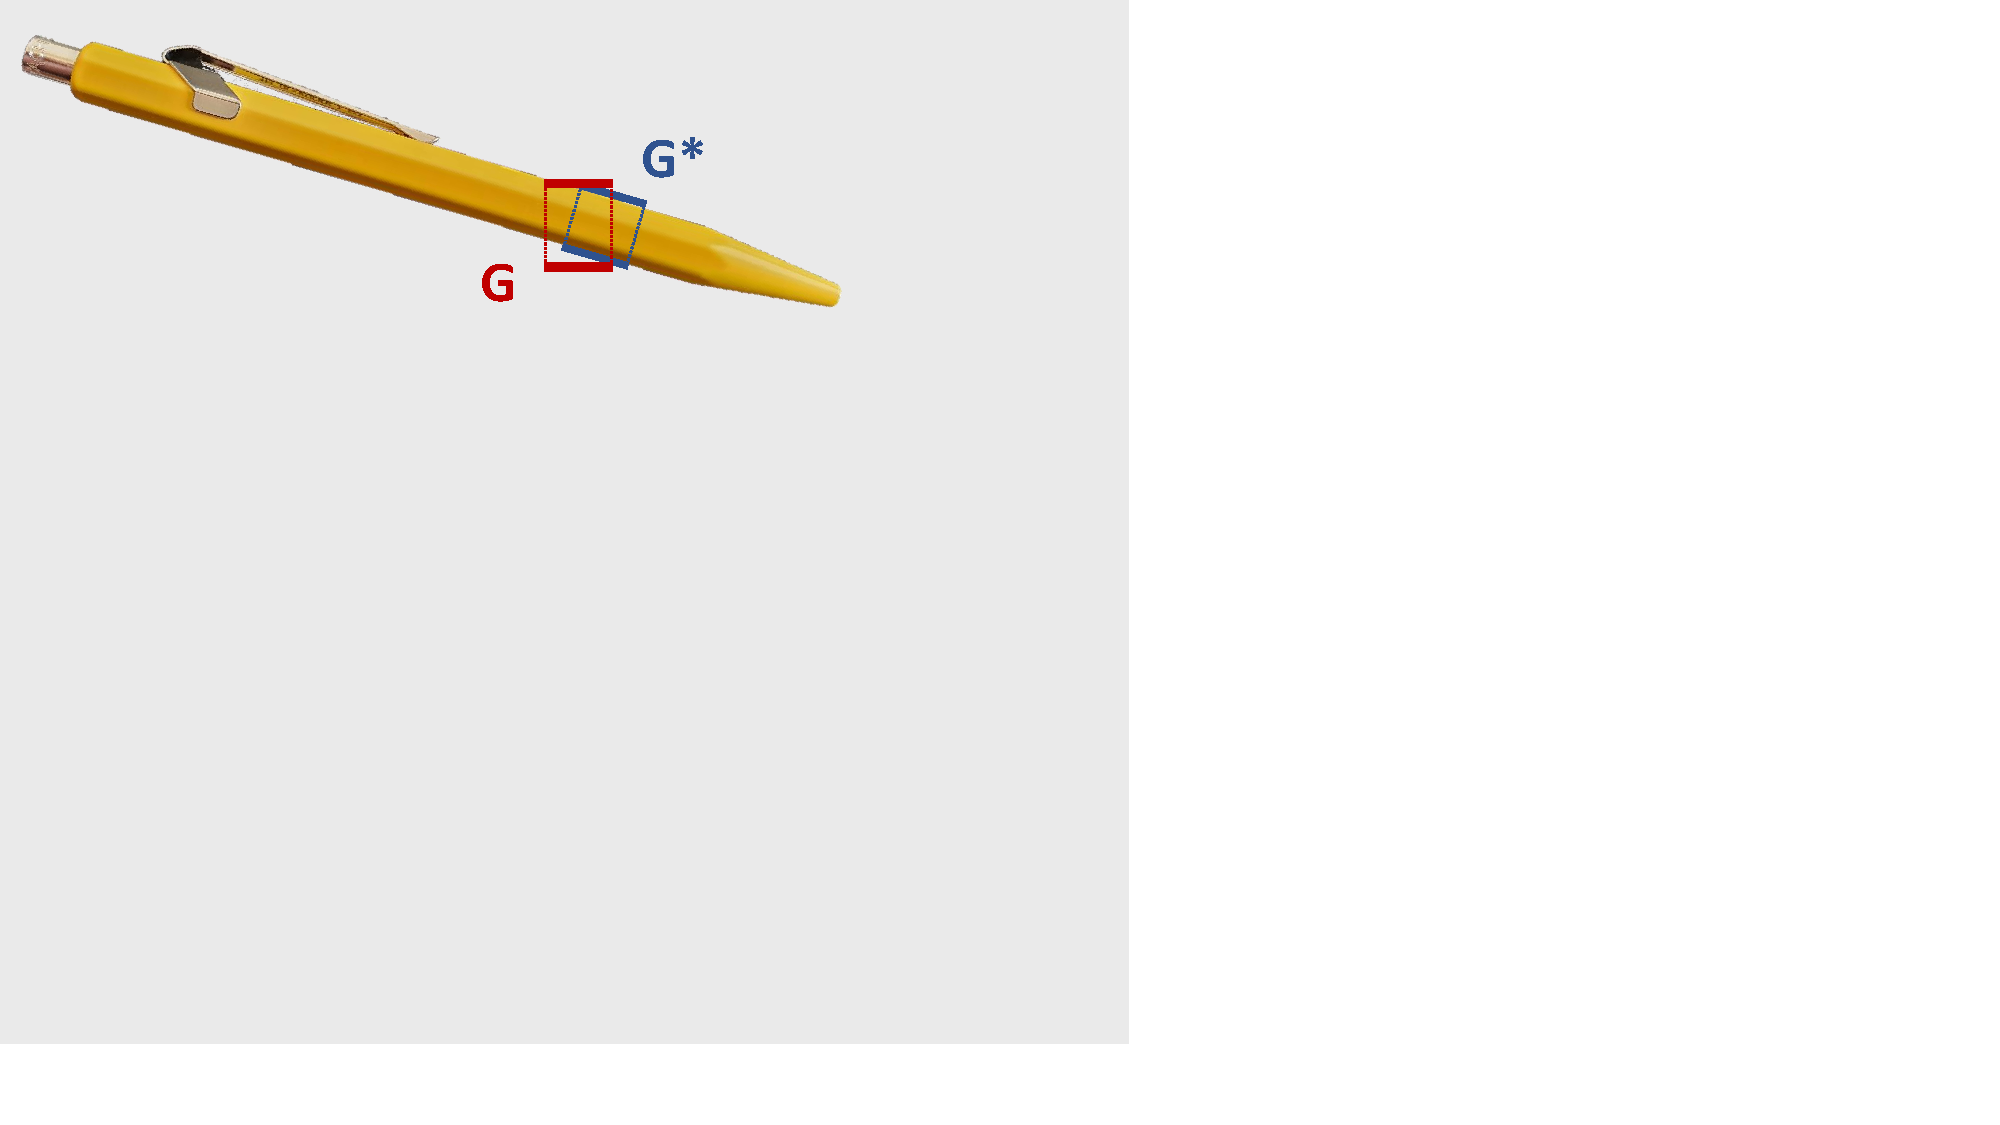
\includegraphics[trim={0cm 12.5cm 17cm 0cm},clip,width=.65\linewidth,angle=0]{Cap2/Figuras/pen_jacquard.pdf}}
	\captionof{figure}{Jacquard threshold representation.}\label{fig:pen_jacquard}
\end{tcolorbox}

The 2D image grasping representation, as already stated, has a lack of fully physical grasping representation. This factor is prominent in point representation since the grasping is only described by its spatial coordinate. Differently, the rectangle representation also includes gripper properties, e.g. finger's width and height, but does not consider friction or any spacial uncertainty, such as the belief map's. The Grasp Path could also be an alternative since it guides several grasp hypotheses to contour the limited space search problem.

It is important to note that, in numerous proposals, the discussed cases are used, and the gripper structure generalisation is not considered (typically, only two fingers are investigated), showing the complexity of this task.

Heretofore, to the best of the authors' knowledge, the most promising representation is formulated by DexNet dataset proposed in~[32-36]. The DexNet is constituted by 3D CAD models labelled with robust grasps for two-finger and suction grippers, i.e., the database was build considering analytical methodologies, iterative algorithm, and simulation interactions. They also included bin-picking and ambidextrous policies. This leads to the idea that the human grasping intuiting is more complicated than only visual representation.


% Ghazei et  al. ideia could be a start ideia to solvenot rigid objects.

\section{Robotic Grasping Approaches}
\label{cap2:related_work:sec:grasping_approaches}

Since the advent of robotic operations, numerous proposals explore the grasping solution idea, from analytical to deep learning approaches. In summary, analytical methods showed to be the first solution to several proposals that achieved exciting results in specific cases. They also formulate the basis used in recent days. However, the main problem is the object grasping generalisation and complexity rise according to the application demand. Currently, the computer science field advances led to machine learning usage that shows to be a potential fashion to deploy effective grasping solutions, until now not reached but with promising results. 

Therefore, the present section is an effort to categorise these strategies over the years and build a structured basis for new studies. This section is organised as follows: first, the analytical methods are explored in Section~\ref{cap2:related_work:sec:grasping_approaches:subsec:analytical_review} following by the data-driven grasping policies, Section~\ref{cap2:related_work:sec:grasping_approaches:subsec:learning_review}. As the deep learning methodology has been the study-case of several state-of-art proposals, this data-driven policy subcategory is presented apart in Section~\ref{cap2:related_work:sec:grasping_approaches:subsec:deep_learning_review}.

\subsection{Analytical Methods}
\label{cap2:related_work:sec:grasping_approaches:subsec:analytical_review}

% A few decades ago, the study of grasp planning was focused on analytical methods. This class of grasping is based on a problem's mathematical model considering the kinematics and dynamics formulations and, strongly depends of the know-how's grasping issue of the specialist, since it is hand-designed methodology. This strategy proved to become complicated, even in the formulation or in computer processing. The challenges arise quickly when more refined is the modelling. Therefore, it is possible to find a significant number of papers that solve specific cases of grasp using the mathematical modelling of the grasp issue. Typically these works are focused in the force- and form-closure properties, wrench space analyses, contact's/friction's equilibrium and stability study. 

% Nguyen [1] proposed and proved some definitions and propositions well suitable and accepted by the actual literature, regarding the creation of three fingers and two fingers gripping contacts in the case of polyhedral and polygon objects. Besides, he proposed an algorithm to perform force closure grasp in these conditions. Nguyen also presents in [2] the development of an algorithm to create a set of stable grasps. In the paper [3], the author proposes an extension of the Nguyen's after a review of analytical analyses, definitions, and propositions while Li et al. [4] offer a different approach, with new analytical definitions, to calculate a three-finger force-closure grasps of 2D objects extending to 3D objects. 

In the beginning, grasping planning was focused on analytical methods. This grasping class is based on a problem's mathematical model considering the kinematics and dynamics formulations. Well-accepted and suitable definitions and propositions regarding form- and force-closure grasping were first explored by~\cite{diziouglu1984mechanics,Nguyen1987_1,Nguyen1987_2}. Subsequently, several proposals extend its grasping stability analyses like~\cite{bicchi1995closure, ponce1995computing, li2003computing} and
the firsts algorithms were proposed, as~\cite{liu1999qualitative,liu2000computing,ding2000computing}. The readers are encouraged to review~\cite{murray1994mathematical,prattichizzo2016grasping} for an embracing grasping analysis.

%TODO: maybe remove the part bellow
% Liu presents a qualitative and a grasp optimized force-closure grasping algorithm in~\cite{liu1999qualitative}. Here, the qualitative analyses are based on the convex theory about the wrenches and are solved with a linear programming method. This paper has an interesting algorithm to evaluate and define the wrenches (the values of the force according to the friction cone) to perform a force-closure but does not estimate the position of the fingers. Trying to formulate a solution to a n-finger gripper, Liu in~\cite{liu2000computing} also proposes an algorithm to estimate all force-closure grasps of an n-finger gripper on a polygonal object. Namely, it defines regions on space to allow a force-closure grasp. Results were evaluated under analytical programming; it was not evaluated using neither a real nor a simulated scenario. The proposal is only for polygonal objects and considers the force-closure analyses taking into account the places of the fingers without defining where to put the finger. Another approach is presented by the authors of~\cite{ding2000computing} who create an optimization algorithm where the position of n-m fingers to perform a force closure grasp to 3D polygonal objects is calculated a priori. 

The analytical methods are applied in specifics cases, with the complexity rising according to the applications' demand. The disparity in mathematical modelling and the real operation is also an issue. Complete and generic analytical grasping solutions are presented by~\cite{liu2004complete,el2009computing} and elucidate these problems. \citeauthor{liu2004complete}~\cite{liu2004complete} propose a complete analytical solution to find a 3D force-closure grasp, frictional or friction-less, for any type of object, including the one with a curved surface. The algorithm combines a local process with a recursive strategy of problem decomposition. First, it inserts n-contacts on the object and recursively tries to find a convex hull that includes the origin. When the search finds a local minimum, the algorithm sets the recursive decomposition method decomposing the problem in sub-problems. Results are analysed over numerical examples without a completely guarantee to find a feasible grasp; an issue is a computational complexity that needs to be evaluated according to the number of contacts used.

\citeauthor{el2009computing}\cite{el2009computing} addressed robust force-closure grasps for generic objects with n-finger hands. To achieve the goal, authors randomly generate $n-1$ fingers position and define the last finger position using the strictly negative linear combination of one of the first generated $n-1$ fingers wrench basis. In this way, the authors reached a faster algorithm, to the detriment of the success rate.

It is important to note that some analytical approaches only aim at estimating the stability of suitable grasps, sometimes called grasping synthesis. However, it is also necessary to determine the best grasp to perform the task. Some analytical methods treat this step as an optimisation problem (\cite{Ciocarlie2009,rakesh2018optimizing}) of some quality measurements. As listed by \citeauthor{Roa2014}~\cite{Roa2014}, a quality measurement can be categorised based on the contact points' position and the hand configuration. An extensive review of these quality methods is presented in~\cite{Roa2014}. These measurements define the grasp analyses optimisation that, in several cases, do not guarantee the grasp determination because of the local minima problem.


\citeauthor{Ciocarlie2009} proposed in~\cite{Ciocarlie2009} to embed the ``Very Fast Simulated Re-Annealing''~\cite{ingber1988}~\cite{kirkpatrick1983} optimisation algorithm, into \textit{Graspit!} simulator~\cite{AndrewT2004}, a widely used grasping planning environment~\cite{morales2006integrated, carvalho2020}. With a 3D pair-wise model, this algorithm tries to reduce the distance of the gripper's contact points and the object's surface evaluating wrist pose and gripper/hand posture. As discussed by \citeauthor{Ciocarlie2009}~\cite{Ciocarlie2009}, the hand posture is defined by \textit{eigengrasps}, a subspace of movement based on how human-generated hand postures. The \textit{eigengrasps} reduces the hand's DOFs based on how humans select appropriate grasps and hand postures. Studies~\cite{Ciocarlie2009,Santello2002} show that humans simplify, unconsciously, the problem with a pattern in the movement. 

Besides the interesting results, the discussed methods demand some unfeasible application efforts, e.g., the optimisation's convergence time could limit the run-time grasping decision process. Thus, the strategy to divide the grasping planning into offline (grasping synthesis) and run-time processes (grasping selection) are used~\cite{carvalho2020}. Typically, the offline procedure generates a list of grasp candidates. The run-time selects the best grasp (under task-oriented capabilities) after matching the sensing data to a dataset. The major problem of these techniques is to know the objects' shape and the gripper's structure. Therefore exceed grasping of novel objects based on already known ones is not possible. This evaluation incorporates the sensing step into grasping planning rather than only perform object localisation and recognition.

%\begin{figure}[h]
%    \centering
%    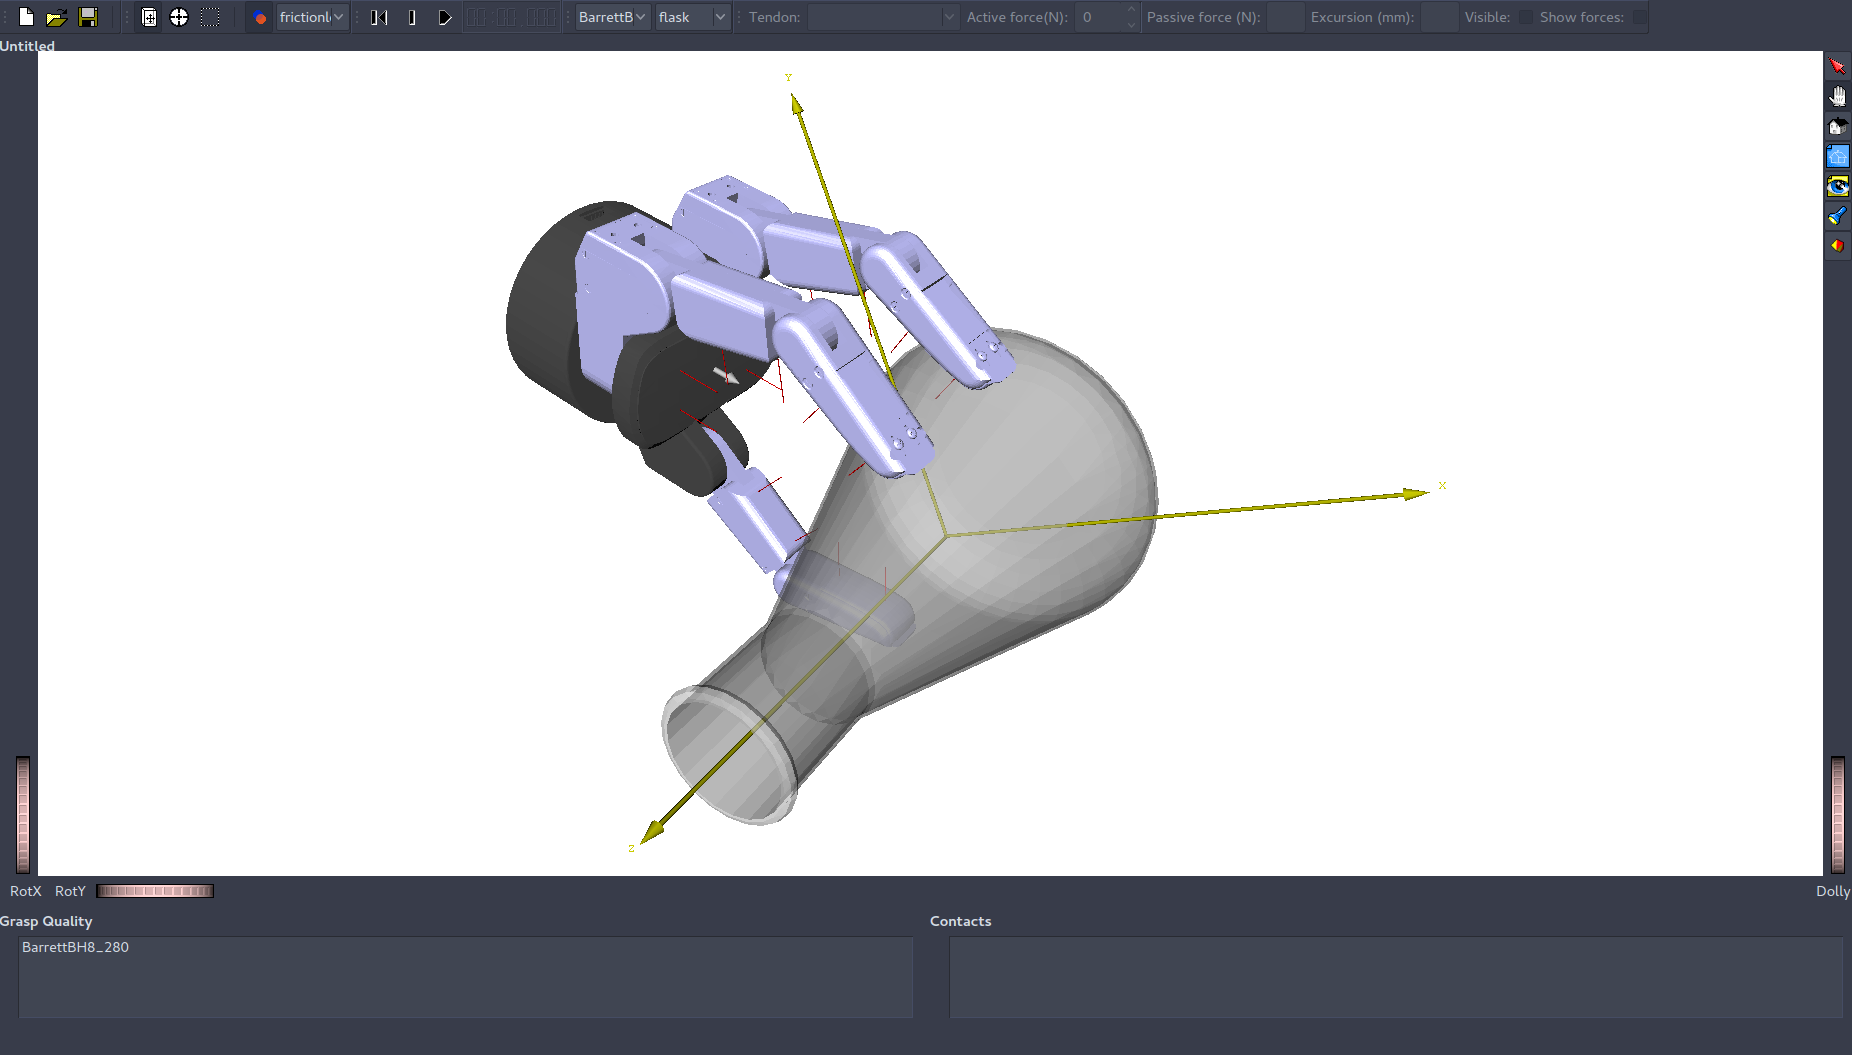
\includegraphics[trim={0 0 0 0},clip,width=1\columnwidth,angle=0]{Cap2/Figuras/graspit5.png} 
%    \caption{``Graspit!'' simulator.}
%    \label{fig:graspit}
%\end{figure}

Once knowing how to grasp spheres, cylinders, cones, and boxes with analytical methods,~\citeauthor{Miller2003}~\cite{Miller2003} investigate the idea to approximate an object to these primitive shapes. \citeauthor{Jain2016} did the same~\cite{Jain2016} by using the point cloud directly. In this context, some approaches use object model decomposition in a set of primitives and execute the ``grasping by parts''. Therefore, the grasping synthesis is simplified, and heuristics methods, associated with analytical approaches as quality control, are proposed. Not only the shape definition is used, but the decomposition tree with superquadrics shapes~\cite{Goldfeder2007}, Reeb graph~\cite{Aleotti2012}, and Medial Axis Transformation~\cite{Przybylski2011} methods are examples trying to solve the related issue. 


% These are the cases of primitive shape, superquadratic and Medial Axis Transformation decomposition methods of~\cite{Miller2003}, \cite{Goldfeder2007}, and  \cite{przybylski2011planning}. Decomposing an object point cloud in primitives and creates two-finger gripper grasps candidates [5] is also an alternative to the previously unknown of the object shape. The grasping by parts is also present in learning policies.

% Verificar se é necessario o seguinte paragrafo.
As discussed in the presented section, the analytical approach has a list of issues that can be summarised as high modelling complexity; high computational complexity; practical inconsistencies; and restricted assumptions. Therefore, the use of learning methods has gained attention, and its development is growing. This fact is verified by the crescent number of papers regarding this theme.

\subsection{Data-Driven Grasping and Learning Policies} 
\label{cap2:related_work:sec:grasping_approaches:subsec:learning_review}

As presented in Section~\ref{cap2:related_work:sec:grasping_representation}, in robotic grasping there is a lack of full representation of the input data, i.e., a partial data representation structure. For instance, a 2D image cannot map the truly grasping interaction, while the simulation could reduce this problem in the loss of applicability. Modelling all physical interaction and noise is unfeasible. However, this issue is not restricted to robots but also presented in humans. Humans can plan to grasp using a stereo-based image with eyes and based on previous experience~\cite{castiello2005neuroscience}. This simple motivation lead studies about learning methodologies to supply these demands, and some pioneer studies can be reviewed in~\cite{Oztop2001, Wheeler2002, Rezzoug2002}.

Indirectly, the optimisation grasping techniques use data or previously known interaction to find a possible solution or refine it~\cite{roa2009finding}. Therefore this kind of methodology can also be included in the data-driven category. However, looking for structured categorisation, this section will only discuss methods regarding classification and machine learning algorithms.

\citeauthor{Pelossof2004}~\cite{Pelossof2004} explore the application of \ac{SVM}, trying to find a regression function to build a map between object shape, grasp parameters, and grasp quality. The authors face the problem of grasp representation in \ac{SL} methodology. Therefore, it was proposed the use of the superquadric objects since these are easily characterised. This approach limits the grasping generalisation only to novel superquadric objects. The ``GraspIt!'' simulator was deployed to generate the database and propose as future work the superquadric combination to characterise more complex objects, later studied by~\cite{Goldfeder2007}. The complexity of feature extraction, while considering different grippers, was also a pioneer study by \citeauthor{dini2000planning}~\cite{dini2000planning}, where a classic Neural Network was proposed to classify an object-agnostic grasping qualitatively. A more recent work~\cite{tenPas} use \ac{SVM} to classify antipodal grasping directly from a point cloud and without recognising it. This paper also evaluates the performance in a densely cluttered environment. The same methodology was used in~\cite{Mahler2017b} but with a grasping proposed database. \citeauthor{Mahler2017b}~\cite{Mahler2017b} also evaluate the use of the Random Forest \ac{SL} algorithm motivated by the work of~\cite{seita2016large}. %However the results do not achieve state-of-art success rates. 

\citeauthor{Saxena2008}~\cite{Saxena2008} was one of the first to explore the supervised grasping learning technique and target object 2D image-based features. They were also motivated by the fact that human object recognition is not related to grasping~\cite{goodale1991neurological}. For this, the authors propose using logistic regression to find grasping point representations and were able to grasp a variety of novel household objects with a success rate of 87.8\%. Based on this, \citeauthor{Jiang2011a}~\cite{Jiang2011a} proposes the use of a two-stage \ac{SVM} classification to detect rectangular grasping contesting the point representation (see Section~\ref{cap2:related_work:sec:grasping_representation}). The first stage is faster and less accurate, while the second stage is more accurate with complex feature detection. Their studies motivate the grasping by an image that later evolves to deep learning policies (Section~\ref{cap2:related_work:sec:grasping_approaches:subsec:deep_learning_review}).

\citeauthor{Trottier2017}~\cite{Trottier2017} use the rectangle strategy, RGB-D images, and \ac{DLSR}, showing a different strategy to \ac{SL} procedure. The authors propose several architectures trying to avoid the big dataset needed for deep learning policies (discussion in Section~\ref{cap2:related_work:sec:grasping_approaches:subsec:deep_learning_review}). They achieved a state-of-art grasping detection rate, but the processing time was not qualified to perform the grasping. %It is also possible to teach a robot grasping by demonstration, in a \ac{LbD} fashion, as related by XXXX. XXX

The \ac{RL} applied to robotic grasping is the focus of studies~\cite{Bernd2002,BaierLowenstein2007, boularias2015learning, platt2007learning} that try to avoid the \ac{SL} approaches shortcomings, e.g., the time-spend to build a labelled database and the limitation of grasping performance according to the supervisor/teacher ability to interpret the physical problem. Typically this class of algorithms is based on trial-and-error approaches focusing on maximising a cumulative reward function. This concept allows an object-agnostic grasping procedure without environment restrictions modelling. However, the major drawback is the time-consuming learning experiments. \citeauthor{boularias2015learning}~\cite{boularias2015learning} use the strategy to push the objects before grasping them in clutter scenes, which was modelled as a \ac{MDP}. A kernel-based \ac{RL} methodologies were implemented, showing that pushing movements can improve grasping performance. Instead of using visual information, \citeauthor{platt2007learning}~\cite{platt2007learning} investigates how to grasp using the contact relative motion model, i.e., using a force sensor as feedback, the algorithm tries to increment small displacement of the finger until reach grasp stability. Modelling it as a \ac{POMDP},~\cite{platt2007learning} tries to solve the optimal control problem using~\ac{RL} methodologies. First, a simulated \ac{RL} was used, which was later transferred to the real robot. This approach is more related to a refined grasping procedure than a grasp synthesis since an initial random grasping point needs to be a priori estimated.

Nowadays, the \ac{SL} and  \ac{RL}  methods were guided to \ac{DL} methodologies based on the promising results of deep architectures applied in robotic task generalisation. Therefore, it is possible to define a distinctive category that will be presented in Section~\ref{cap2:related_work:sec:grasping_approaches:subsec:deep_learning_review}, the deep learning grasping.


%TODO: ler mais papers daqui... Learning: LbD; RL; SL; UL ....

\subsection{Deep Learning Grasping Policies}
\label{cap2:related_work:sec:grasping_approaches:subsec:deep_learning_review}


The new deep learning policies and deep network architectures have leveraged computer vision detection tasks, as the object recognition problem proposed by ImageNet Large Scale Visual Recognition Challenge~\cite{imagenet_challenge}. In this field, the advent of deep \ac{CNN}~\cite{krizhevsky2012imagenet}, and the constant improvement of its architecture shown promising results. These results have been drawn the attention of robotic researchers that seek to apply the generalisation capability of these networks in the grasping issue, as can be seen by the competitor's proposals of Amazon Picking Challenge~\cite{amazon_challenge}.

\citeauthor{Lenz2015}~\cite{Lenz2015} was one of the first to investigate the \ac{DL} in grasp planning. In their proposal, a grasp rectangle~\cite{Jiang2011a} is elected after a two-stage cascade detection learning network using RGB-D images. The first layer, less accurate, is responsible for learning a large number of direct features from the view, and the second layer selects the best grasp position using these features. The input image is gathered using a sliding window technique. However, this strategy compromises the real-time application, as reported by
~\cite{Redmon2015, Guo2017,Chu2018}. \citeauthor{Lenz2015}~\cite{Lenz2015} verified that the \ac{DL} improve the learning process since a hand-engineering feature modelling was not needed. Another precursor \ac{DL} work was proposed by \citeauthor{Redmon2015} in~\cite{Redmon2015} which applied the AlexNet~\cite{krizhevsky2012imagenet} \ac{CNN} architecture to grasping prediction.  \citeauthor{Redmon2015}~\cite{Redmon2015} explored the Transfer Learning concept between \ac{DL} applications, latterly used by works~\cite{Kumra2017,TenPas2017, Chen2019,Mahler2017d,Zeng2019,Chen2020}, and verified that this approach supports the training process preventing over-fitting due to the limited labelled database size. Their proposal uses a complete RGD image to direct regression to rectangle grasp. The strategy of replacing the blue channel with depth is also verified in subsequent works~\cite{Kumra2017,Chen2019,song2020novel} that adapt the image classification \ac{CNN} architectures to the grasping problem. The authors affirm that adding an extra channel in these architectures avoids the pre-training phase with the image classification dataset. Therefore, the grasping architecture was pre-trained with object classification of~\cite{imagenet_challenge} and also evaluated by the hypothesis to classify an object before grasping it. The authors achieved an almost $85\%$ of detection success rate (see Table~\ref{tab:met_state_of_art}), however when the proposal is exceeded to real grasping a reduction in the efficiency is related, as can be verified by the results achieved in~\cite{Watson2017} and~\cite{Chu2018}.

After the advent of ResNet \ac{CNN} architecture~\cite{he2016deep}, \citeauthor{Kumra2017}~\cite{Kumra2017} propose its use in grasping in two different modalities: uni-modal with direct RGB or RGD data, and multi-modal with RGB and three-dimensional depth data, therefore two ResNet networks. In both cases, the ResNet layer was responsible for extracting the features that were classified as good grasping by a fully connected layer. This multi-modal strategy is also verified in papers as~\cite{Guo2017}. However, \citeauthor{Guo2017}~\cite{Guo2017} use tactile data motivated by the fact that the grasping is not only a classification image-like problem.  It was expected to model the grasp stability during the training process indirectly. With a deep visual network and a deep tactile network, the hybrid architecture achieved an $89\%$ detection success rate. The practical grasping performance was tested by \citeauthor{Chu2018} in~\cite{Chu2018} achieving a success rate of $81\%$ (see Table~\ref{tab:met_state_of_art}). \citeauthor{Chu2018}~\cite{Chu2018} also proposed the use of  ResNet and VGG-16 \ac{CNN} architecture with candidate regions to a focused feature search (motivated by \ac{RPN}). With this approach, the authors achieved interesting detection rates with practical evaluation, see Table~\ref{tab:met_state_of_art}. 

The ResNet is also used by \citeauthor{Ghazaei2019}~\cite{Ghazaei2019} in a \ac{FCN} architecture which, instead of finding a regression from RGB images to rectangle grasp, direct output a Grasp Belief map (see Section~\ref{cap2:related_work:sec:grasping_representation}). However, to evaluate and train their network, it was used the \ac{CGD} which caused~\cite{Ghazaei2019} to ``translates'' the belief map in rectangle grasping, compromising the truly potential evaluation. Other examples of deep \ac{CNN} applied to the grasping problem is the LeNet of~\cite{TenPas2017} that use direct Point-Clouds of the scene to estimate feasible antipodal grasps, and the DarkNet53 (from YoloV3)~\cite{Chen2020} used to estimated the grasp path discussed in Section~\ref{cap2:related_work:sec:grasping_representation}. 

It is possible to notice that a better grasp success rate is more dependent on a complete grasping modelling than only the Deep Network architecture strategy. This fact can be seen by the DexNet project's design which confirms that the grasping planning is a more complex task than only a classification image-like problem. \citeauthor{Mahler2016} start the DexNet project~\cite{Mahler2016} designing an algorithm to create a more reliable database called DexNet 1.0. This database, interactively generated, is composed of a set of parallel-jaw grasps associated with the object's 3D model. Each grasp is labelled with a probability of force closure under uncertainty in object pose, gripper pose, and friction coefficient. In the following works, the database evolved, including: scenario constraints, as planar base surface; different scene points of view; bin-picking and dense clutter scenarios; and ambidextrous policies to select the appropriate gripper (suction or two-finger). With the DexNet, a \ac{GQ-CNN} was proposed to select and define a robust grasp configuration in single object grasping and bin-picking. Nevertheless, the authors encounter challenges in grasp flexible, porous objects and with loose packing.

As shown in this section, building a sufficient size labelled database is the main drawback of \ac{DL} policies. Even though a large database could be available,  assess if the labelled database modelling includes all necessary practical assumptions is difficult. Therefore, some proposals try to overcome this problem by generating data through practical experiments or using \ac{DRL} methodologies. That is the case of \citeauthor{Pinto2015}~\cite{Pinto2015} that generates a proprietary database with 50k tries of random robotic grasping and mapping them to the rectangle database. For the authors, the image ground-truth and the simulated interactions database are questionable. However, their reduced success rate probably is due to their grasping representation simplification. Although their proposal is a \ac{SL}, the authors face a similar problem of \ac{RL} methodologies: the time spent by the database physical try-and-error.

% There exists several \ac{DCNN} architectures that can be applied into a grasping problem, like the discussed AlexNet, ResNet, VGG-16, LeNet~\cite{TenPas2017} and DarkNet53~\cite{Chen2020} and all the results lead to the following interpretation: the grasp representation, Section~\ref{sec:grasping_representation}, and database build plays an important role in grasping success rate. Focusing on that, the DexNet~\cite{Mahler2016, Mahler2017b, Mahler2017d, Mahler2017, Mahler2019} project achieved interesting results including two-fingered, suction grasping, bin-picking, and ambidextrous policies. ...

% {TODO: falar que nao antigiram resultado bon para multiplo objectos e likar com paper do 6DOF}

% Maybe insert images from these papers ...

The authors of~\cite{Zeng2019} propose the direct use of RGB-D pixel-wise to infer, with \ac{FCN}, affordances grasping instead of classical mapping to grasping parameters. In a grasp-first-then-recognise workflow, the authors mapped affordance maps of a discrete set of grasping primitives for suction and two-finger grippers. With this direct approach, as related by~\cite{Zeng2019}, a faster, reliable, and able to learn complex grasping rules was verified. \citeauthor{Zeng2018} also investigate in~\cite{Zeng2018} a Deep Reinforcement Learning methodology to evaluate the synergy between push and grasp, achieving interesting results to adversarial clutter scenarios without previous knowledge of the object's shape. It was proposed the use of two \ac{FCN}, trained by simulated trial-and-error experiments and Q-learning approach. Studies regarding complex object formats are needed.

Using a monocular camera, \citeauthor{Levine2018}~\cite{Levine2018} evaluated the use of a \ac{CNN} and a servomechanism to end-to-end grasping planning, in a visuomotor control fashion. The visuomotor approach allows a direct map from visual sensing, gets continuous environment cues, and reacts to adversarial conditions and perturbations, i.e., more appropriate to dynamic environments~\cite{morrison2020learning}. However, a drawback in end-to-end is regarding the portability since the algorithm needs to be re-adjusted according to the robot. In these methods, the control loop entirely depends on the system in usage. Other strategies of this methodology can also be check in~\cite{james2017transferring} and~\cite{viereck2017learning}. \citeauthor{Levine2018}~\cite{Levine2018} confronted the high effort to build a reliable self-supervised database, similar to~\cite{Pinto2015} using several robots during two months to teach their grasping prediction \ac{CNN}. The authors of~\cite{Pinto2015,Levine2018} noticed that their approach matched deep \ac{RL} methodologies requisites. %TODO: verificar!!!!  %The visuomotor and the \ac{RL} showed some interesting results however, the effort needed to create the system is its main drawback and, improvement in this field is the focus of several state-of-art-studies. 

\section{Conclusion}
\label{cap2:related_work:sec:grasping_approaches:subsec:conclusion}

Several works were reported in the reviewed literature showing the scientific community's significant effort to solve the robotic grasping issue. This chapter elucidated how complex and deep is the grasping planning problem. It also presented some of the several works on the area, the main contributions, and how robotic grasping evolved and still evolving over the past decades: from wrench space heuristics to {DL} policies, i.e., to analytical to deep machine learning methodologies. 







%This paper also discussed and presented the motivations that allow the authors to formulate some fair and transparent definitions of the results' assessment. With this, an attempt was made to standardise the grasping results metrics simplifying the research community's comparison. The paper also discussed and enumerated some future work ideas based on the review, guiding and clarifying some next steps in robotic grasping strategies.




\chapter{Grasping Evaluation Proposal}
\label{cap3:grasping_eval}

After the grasping solution development, researchers encounter a common problem: how to evaluate the proposed methodology? The robotic grasping is typically composed of a complex system that includes, in most cases but not essential, the following issues: object sensing and identification; pose estimation; grasping detection; grasping selection; trajectory planning; force and stability estimation; collision avoidance, among others. All these components have their errors related and directly affect grasping performance. For instance, robotic manipulators and 3D sensors have intrinsic's action and measurement errors, respectively. Besides, estimation and planning algorithms also have considerable accuracy errors and variations.

Regarding this evaluation shortcoming, some authors proposed well-accepted assessments in the literature. These include point and rectangle grasping representation comparing with distance threshold and Jacquard index in \ac{DL} policies' database ground-truth. The Epsilon and Volume wrench space metrics are also other examples applied to analytical grasping methodologies (Section~\ref{cap2:related_work:sec:grasping_representation}). Although these metrics are focused on a specific grasping step (rectangle and point comparison metric in the detection, and Epsilon and Volume in physical active-pair interaction), they do not reflect the practical robot grasping performance. Some papers specify their own evaluation metric to a robotic grasping in a real scenario, but it is still difficult for readers to have a comparative review of the results. Therefore, these motivations allow us to formulate some fair and transparent definitions of the results' assessment. Thus, readers can have a clear idea of what is in the comparison between the methods. With the grasping problem steps presented in Figure~\ref{fig:eval}, it is defined four grasping evaluation success rate criteria: Grasp Prediction, Grasping Reaching, Grasping-Hold, and Handling Grasping.

\begin{figure}[h!] %because of cas-sc
\begin{tcolorbox}
% \centerline{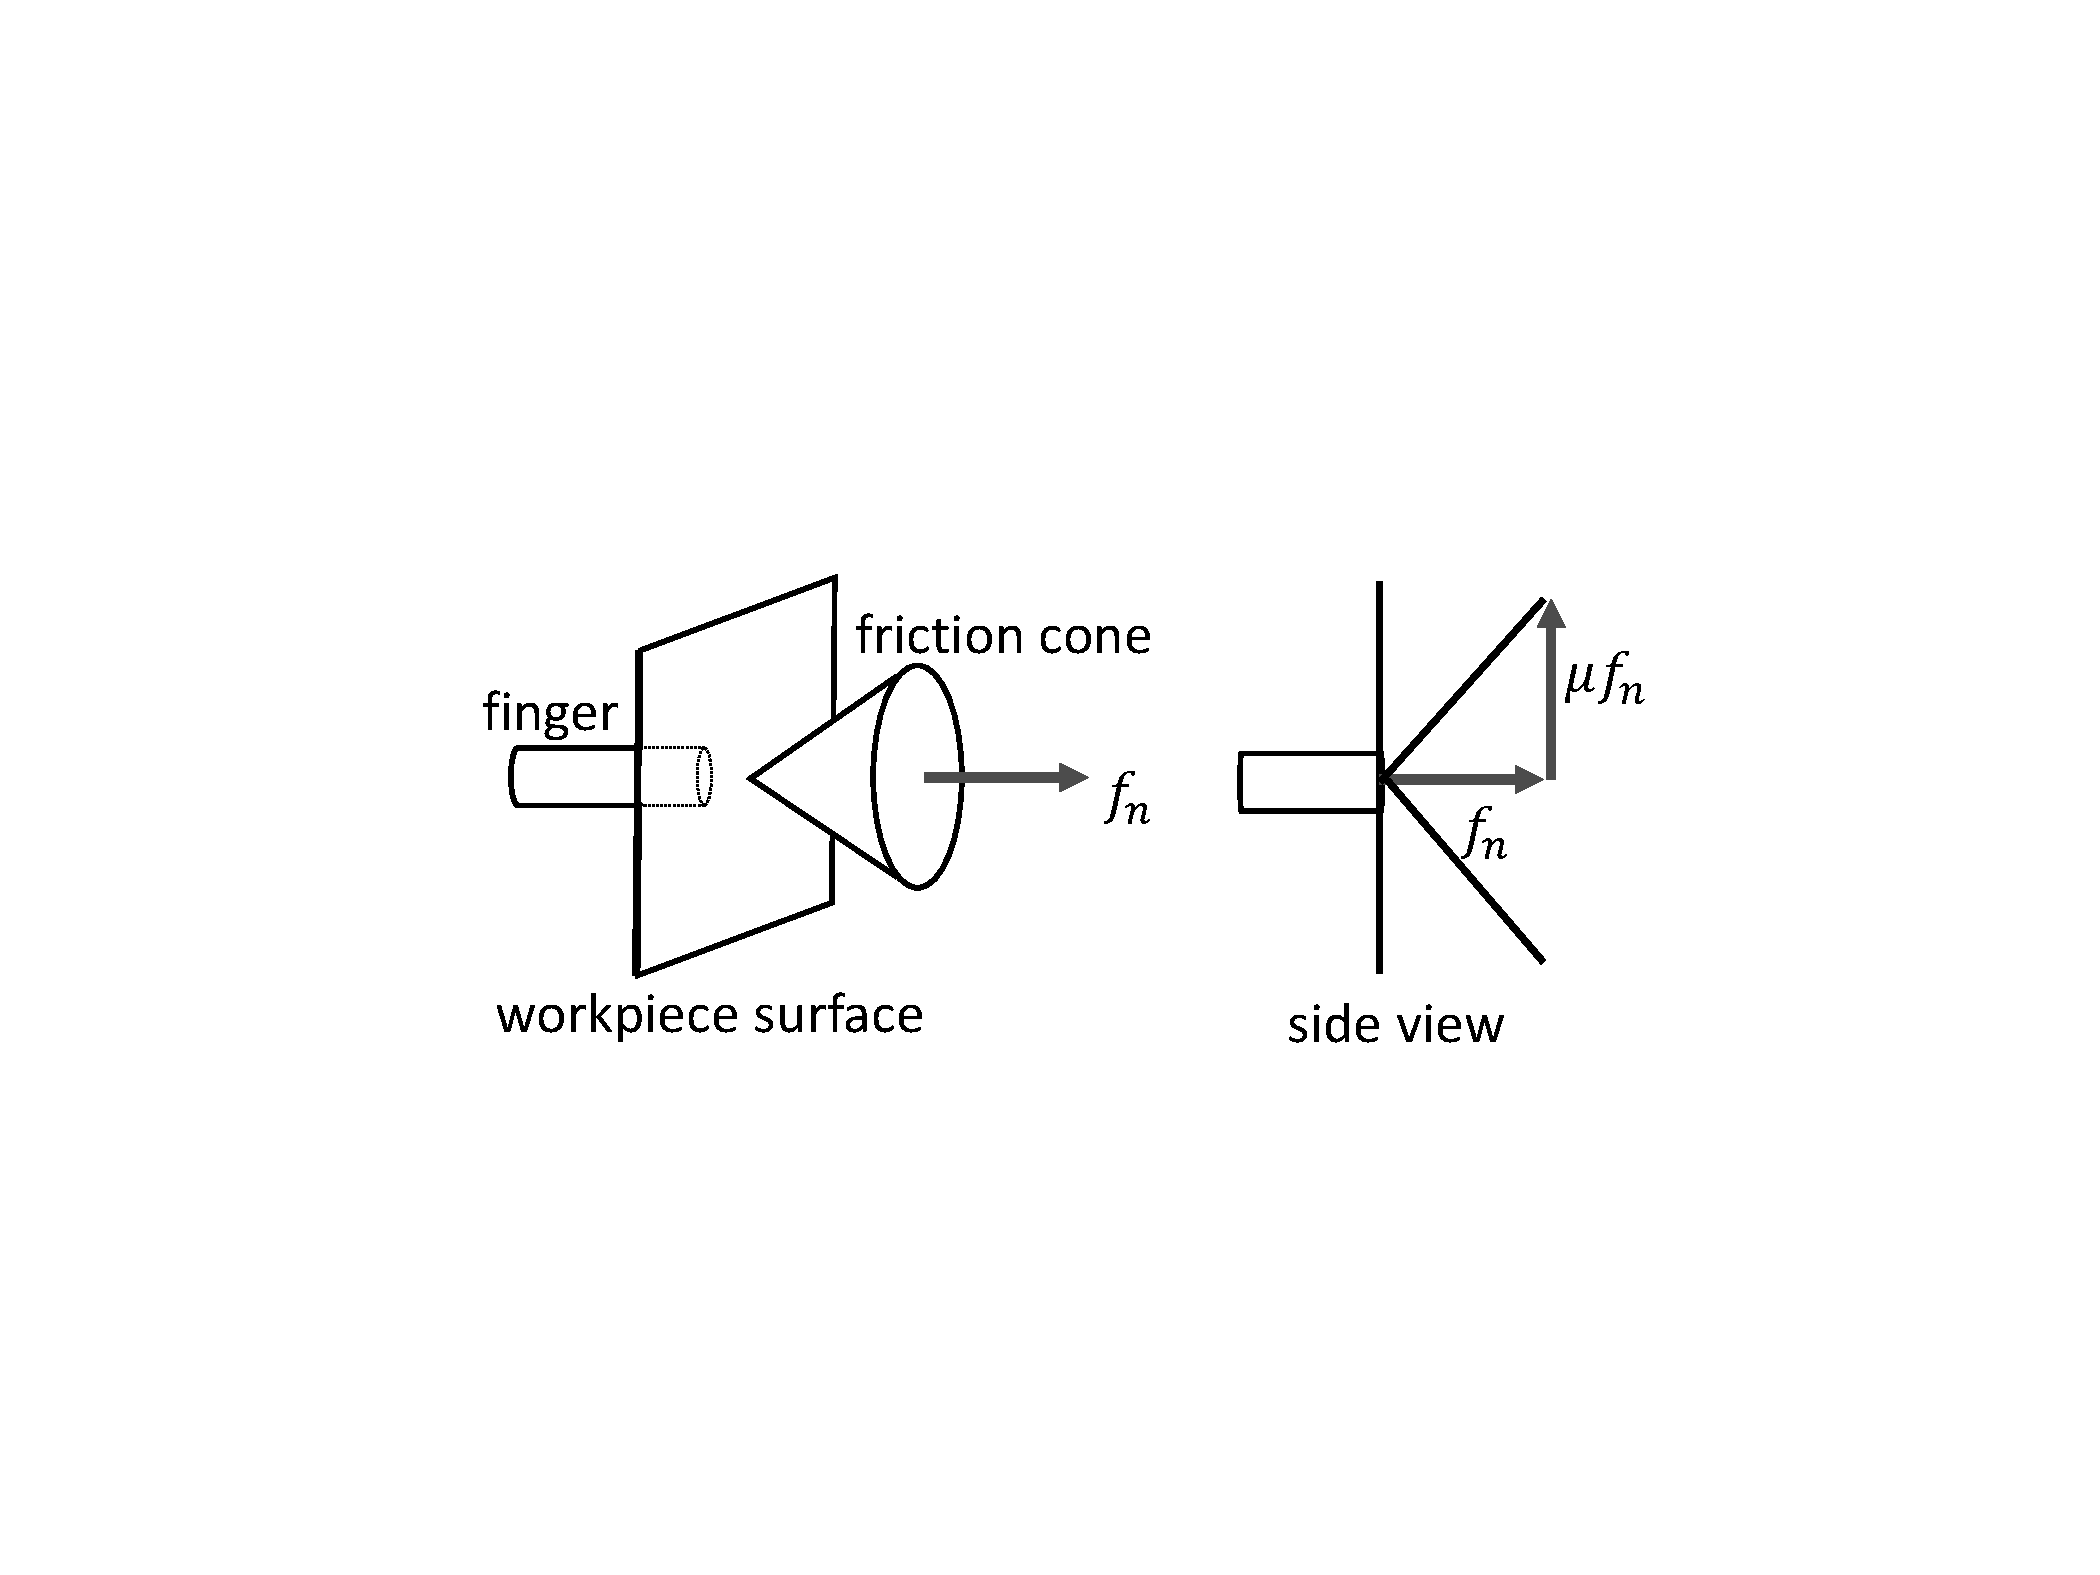
\includegraphics[trim={7cm 8cm 7cm 9cm},clip,width=1\linewidth,angle=0]{Cap2/Figuras/friction_contact.pdf}}
\centerline{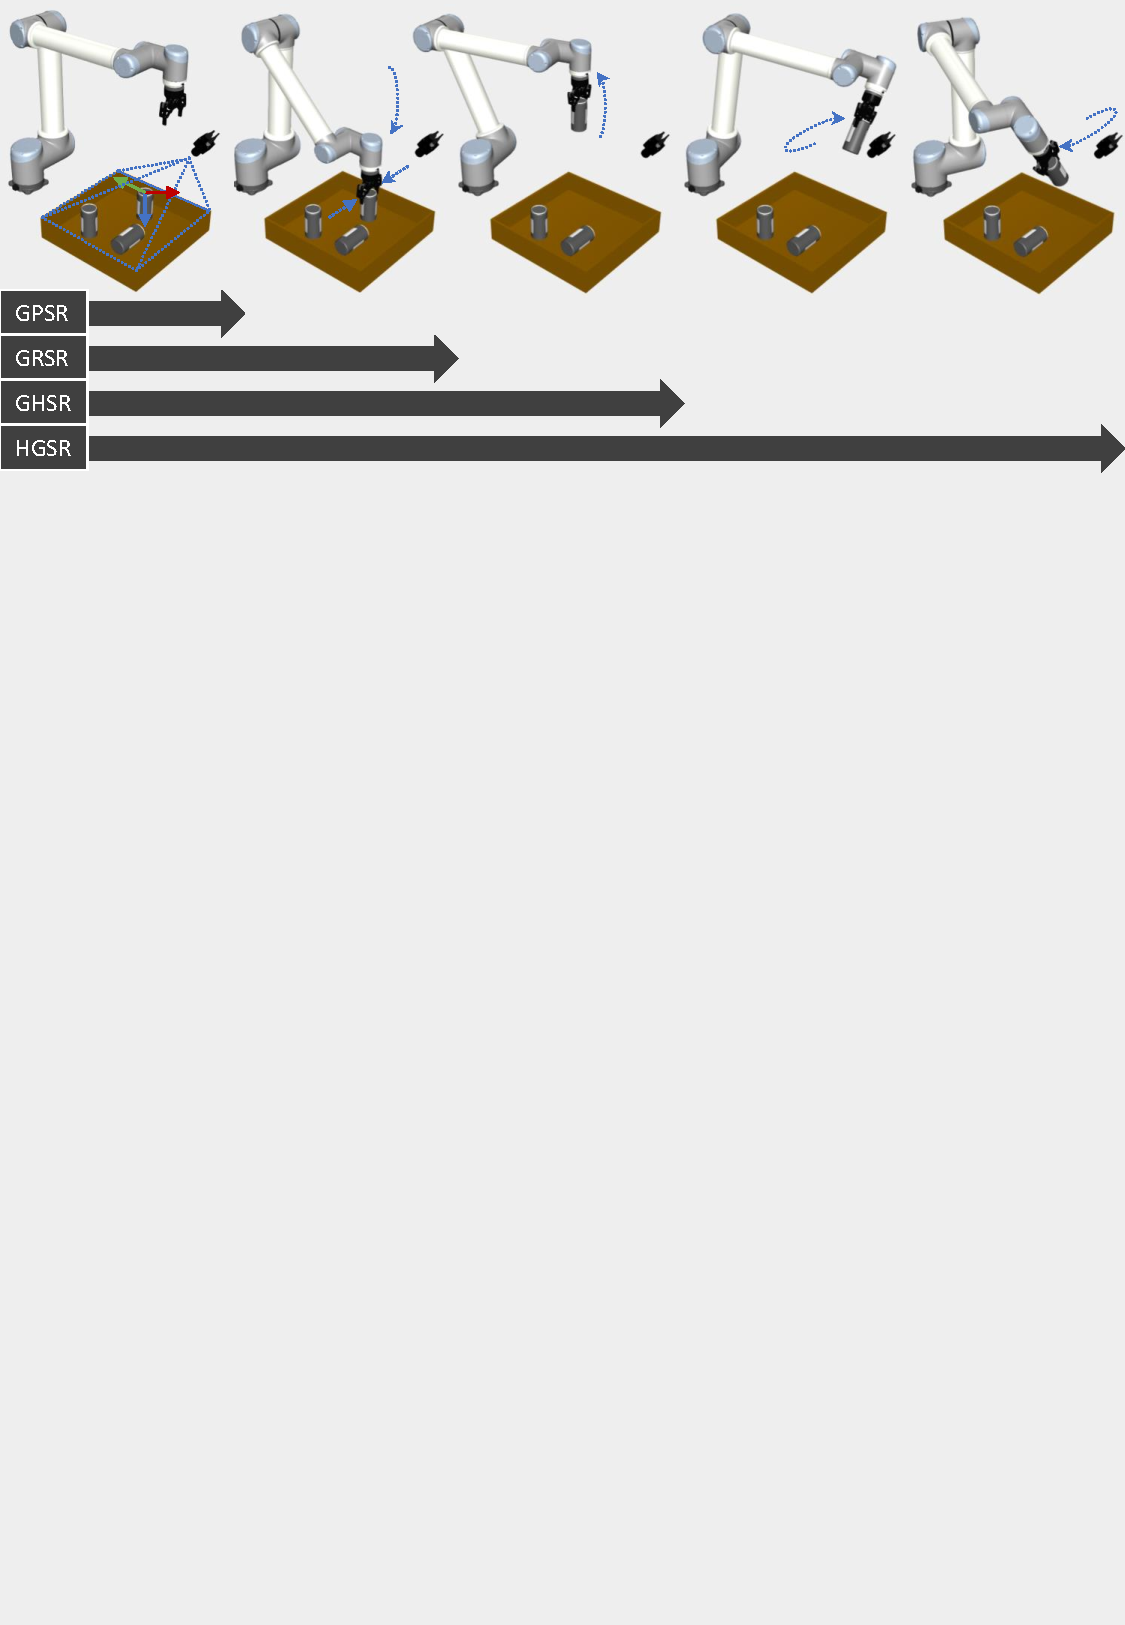
\includegraphics[trim={0cm 19.5cm 0cm 0.07cm},clip,width=1\linewidth,angle=0]{Cap2/Figuras/teste_2.pdf}}
\end{tcolorbox}
\caption{Proposed grasping assessments and their progression timeline. The categories evaluate the grasping performance in different levels based on the complexity of the actions, indicated by the arrows timeline. Each class englobes the prior class resulting in an ascending complexity order from Grasp Prediction (GPSR), Grasping Reaching (GRSR), Grasping-Hold (GHSR) to Handling Grasping success rates (HGSR). The last two successive images describe the 6DOF movements of HGSR.}
\label{fig:eval}
\end{figure}

\section{Grasping Prediction Success Rate}
\label{cap3:grasping_eval:sec:gpsr}

The \ac{GPSR} allows the grasp prediction (or detection) evaluation that consists of the grasp pose estimation generated by methodologies such as the \ac{DL} with \ac{CNN}~\cite{Mahler2019} and the \ac{SANN} optimization technique~\cite{AndrewT2004,carvalho2020}.

In these methods, single or multiple grasping poses are compared with ground-truth and an evaluation of how the graspable estimation is likely to perform, with success, given sensing type: RGB image, Depth map, or Point-Cloud. It is necessary to define if the object is previously known or, in case of \ac{SL} methodologies, if the metric considers sensing-wise (an object sensing data was already presented in the learning phase but with different perspectives from the test case) or object-wise (the object sensing data was never shown in the learning phase). The ground-truth used could be based on a labelled database, such as the \ac{CGD} database, or human supervision considering the user task expertise. Comparison metrics examples are the Euclidean distance between grasping points, the Jacquard threshold to rectangle grasping, the wrench space volume, or the $\epsilon$-value into a simulation procedure. These methods are discussed in Section~\ref{cap2:related_work:sec:grasping_representation}.

This class of success rate is prevalent in deep \ac{CNN} policy proposals, like~\cite{Redmon2015,Kumra2017,asif2018ensemblenet,song2020novel}.Usually, when applied in experimental cases, it has its success rate impaired since it does not evaluate the grasping interaction either the grasping related movements as can be seen in~\cite{Chu2018}.

The processing time related is \ac{GPT}. Normally in this step, the convergence time could be higher in analytical/optimization methods (Section~\ref{cap2:related_work:sec:grasping_approaches:subsec:analytical_review}) demanding a split in grasping planning: offline (\ac{Offline-GPT}) and run-time (\ac{Run-GPT}) approaches~\cite{carvalho2020}. In \ac{DL} policies it could require swap the processing unit from \ac{CPU} to \ac{GPU} generating the \ac{CPU-GPT} and \ac{GPU-GPT}, respectively.

The \ac{CPU-GPT} and \ac{GPU-GPT} could be directly compared; however, the unit processing explicitly shows the hardware requirement. In real applications, an ideally need is the \ac{CPU-GPT}  since \ac{CPU} is cheaper and simpler to be implemented and used, even though this achievement looks like far to state-of-art literature. It is important to note that, with the development of cheaper \acp{GPU} and accessible and straightforward libraries, like CUDA~\cite{cuda}, this could be an irrelevant issue.


\section{Grasping Reaching Success Rate} 
\label{cap3:grasping_eval:sec:grsr}

Suppose a grasping task where sensing is performed, followed by the grasp detection, grasp movement, and gripper's close over the grasp point. In this case, the \ac{GRSR} evaluates the methodology performance considering the deviation from the generate grasping pose and the active grasp point, i.e., the gripper's closing over the object. Therefore, it is a complete way to check the validity of error propagation in a practical scenario compared to \ac{GPSR}, which only evaluates mathematical modelling parameters where practical inconsistencies can appear. This metric includes the accuracy of object sensing, estimation, grasp prediction, grasping acting and can be specified by these error variations. Works like~\cite{moreira_2016} consider this intermediate error assessment, classified as valid or not by a kNN algorithm, critical to a reliable grasping since the \ac{GRSR} defines a starter error that can affect the next task steps.

However, not all physical interactions between the active-pair are evaluated, and only the grasping position precision and friction are appraised. It is important to note that small deviations could generate stable grasps, and a vast number of sensors, robotics manipulators, and grippers have a reduced intrinsic's error. Therefore in a controlled environment, the evaluated error could be small. Also, in referred conditions, the estimation, sensing, and planning algorithms must be designed with caution not to generate high error rates, i.e. a complete error propagation from \ac{GPSR} into \ac{GRSR}. This metric could be useful in precision grasping applications where the contact grasping region is necessary or the grasp slippage avoiding is critical. In addition, the \ac{GRSR} could be considered a filter to eliminate a significant pose grasping error and evaluate its propagation in the overall system.


\section{Grasping-Hold Success Rate} 
\label{cap3:grasping_eval:sec:ghsr}

The \ac{GHSR} allows a complete grasping evaluation criteria. It is considered a robotic grasping application where sensing is performed followed by grasp detection, grasp movement, gripper close over the grasp point, lift the object and hold it for a period. Besides evaluating the error propagation in a practical scenario, as \ac{GRSR} does, it is possible to check the equilibrium of the grasping performance over perturbations and physical interactions, e.g., the slip, wrench space configuration, and the gravity force actuation. This metric could also be evaluated according to object and gripper material friction changes and holding time variation. It important to note that this category excludes the unintentionally grasp that could happen in cluttered and/or bin-picking grasping operations.

\section{Handling Grasping Success Rate}
\label{cap3:grasping_eval:sec:hgsr}

Although \ac{GHSR} could be enough to define a good grasping approach, a more realistic grasping evaluation criteria is the \ac{HGSR}.  Besides including all considerations of \ac{GHSR},  the \ac{HGSR} evaluates the grasping holding of an object and moving it in all robot's DOFs, checking its stability. This metric is relevant for practical scenarios since, in the industry, the work cycle is an important parameter to evaluate. The \ac{GHSR} could be assessed according to the robot movement's speed and acceleration variation, besides the work cycle. It is also possible to include the object's placing movement. However, any analysis of this procedure could confront a new task apart from grasping.

\section{Discussion}
\label{cap3:grasping_eval:sec:discussion}

Aiming to deploy the proposed grasping evaluation in currently state-of-art and, stabilising a fair comparison about the literature solutions, Table~\ref{tab:met_state_of_art} presents some grasping approaches and their performance. This table is a guiding tool, and the readers are encouraged to check the source since, besides the specific restriction used in each paper's database that can lead to an unfair comparison, the results presented here are an elucidation give the described conditions: 

\begin{enumerate_jp}
    \item All assessments are restricted to agnostic-grasping (the current challenge in grasping) even though some paper also present better results evaluation with previous knowledge of object shape; 
    \item Only object-wise metric are presented since the object-agnostic is considered;
    \item For tests where the author categorise the objects, the most ``typical'' class is selected in the present table;
    \item The column ``Model Interaction'' indicates if any model interaction is needed to synthesised or selected a grasp (it does not include the database build step of results evaluation) since this affects the grasping performance convergence time;
    \item It is only considered static scenario;
    \item Each methodology was classified according to proposed Grasp Evaluation, Section~\ref{cap3:grasping_eval}. Therefore, if realised, it is presented the most complex category in descending order of: \ac{HGSR}, \ac{GHSR}, \ac{GRSR} and \ac{GPSR}. 
\end{enumerate_jp}


%clutter and isolated scenarios are specified

%%\clear
% Please add the following required packages to your document preamble:
% \usepackage{graphicx}
% \usepackage[table*,xcdraw]{xcolor}
% If you use beamer only pass "xcolor=table*" option, i.e. \documentclass[xcolor=table*]{beamer}


% \usepackage{geometry}
\newgeometry{paper=a4paper,hmargin={1cm,1cm},offset={0cm,-3.5cm}, bottom=-5cm} 

\begin{table*}[h!]
%\vspace{-8.5em}%

\resizebox{0.755\textwidth}{!}{%
\centering
\caption{Object-agnostic grasping methodology proposals and their performances.}
\label{tab:met_state_of_art}
\begin{threeparttable}

\begin{tabular}{cccccccccc}
\hline
\rowcolor[HTML]{C0C0C0} 
%Year &
  \textbf{Methodology Description} &
  \textbf{\begin{tabular}[c]{@{}c@{}}Clutter\\ Scenario\end{tabular}} &
  \textbf{\begin{tabular}[c]{@{}c@{}}Gripper\\ Approach\end{tabular}} &
  \textbf{\begin{tabular}[c]{@{}c@{}}Grasping\\ Representation\end{tabular}} &
  \textbf{\begin{tabular}[c]{@{}c@{}}Model\\ Interaction\end{tabular}} &
  \textbf{\begin{tabular}[c]{@{}c@{}}Sensing\\ data type\end{tabular}} &
  \textbf{\begin{tabular}[c]{@{}c@{}}Processing\\ Time\end{tabular}} &
  \textbf{\begin{tabular}[c]{@{}c@{}}Result\\ Class\end{tabular}} &
  \textbf{\begin{tabular}[c]{@{}c@{}}Performance \\ (Success Grasps)\end{tabular}} \\ \hline
%2004 &
  \begin{tabular}[c]{@{}c@{}}SVM with superquadric \\ shape objects description~\cite{Pelossof2004} \end{tabular}&
  No &
  Generic* &
  Eigengrasp &
  Yes &
  N/R &
  N/R &
  N/R &
  N/R \\
\rowcolor[HTML]{C0C0C0}
%2008 &
  \begin{tabular}[c]{@{}c@{}}Proprietary learning algorithm with\\ logistic regression and image~\cite{Saxena2008}\end{tabular} &
  No &
  Two-Finger &
  Point &
  Yes &
  RGB &
  N/R &
  GHSR &
  87.80\% \\
%2008 &
  \begin{tabular}[c]{@{}c@{}}Proprietary learning algorithm with\\ logistic regression and image~\cite{Saxena2008}\end{tabular} &
  Light &
  Two-Finger &
  Point &
  Yes &
  \begin{tabular}[c]{@{}c@{}}Gray Scale\\ and Depth\end{tabular} &
  N/R &
  HGSR &
  80.00\% \\
\rowcolor[HTML]{C0C0C0} 
%2011 &
  Two-Stage SVM-rank classification~\cite{Jiang2011a} &
  No &
  Two-Finger &
  Rectangle &
  No &
  RGB-D &
  50.000s &
  GHSR &
  87.90\% \\
%2015 &
  Two-stage deep network~\cite{Lenz2015} &
  No &
  Two-Finger &
  Rectangle &
  No &
  RGB-D &
  13.500s &
  GHSR &
  84.00\% \\
\rowcolor[HTML]{C0C0C0} 
%2015 &
  \begin{tabular}[c]{@{}c@{}}Single grasp based on AlexNet\\ direct regression~\cite{Redmon2015}\end{tabular} &
  No &
  Two-Finger &
  Rectangle &
  No &
  RGD &
  0.076s &
  GPSR &
  84.90\% \\
%2015 &
  Multi grasp detection based on AlexNet~\cite{Redmon2015} &
  No &
  Two-Finger &
  Rectangle &
  No &
  RGD &
  0.076s &
  GPSR &
  87.10\% \\
\rowcolor[HTML]{C0C0C0} 
%2016 &
  \begin{tabular}[c]{@{}c@{}}K-NN classification of proprietary dataset and\\ histogram of oriented gradient description~\cite{Pinto2015}\end{tabular} &
  Light &
  Two-Finger &
  Rectangle &
  No &
  RGB-D &
  N/R &
  GPSR &
  69.40\% \\
%2016 &
  \begin{tabular}[c]{@{}c@{}}Linear SVM of proprietary dataset and histogram\\ of oriented gradient description ~\cite{Pinto2015}\end{tabular} &
  Light &
  Two-Finger &
  Rectangle &
  No &
  RGB-D &
  N/R &
  GPSR &
  73.30\% \\
\rowcolor[HTML]{C0C0C0} 
%2016 &
  CNN with proprietary database~\cite{Pinto2015} &
  Light &
  Two-Finger &
  Rectangle &
  No &
  RGB-D &
  N/R &
  GHSR &
  66.00\% \\
%2016 &
  "Common-Sense" analytical heuristic~\cite{Pinto2015} &
  Light &
  Two-Finger &
  Rectangle &
  No &
  RGB-D &
  N/R &
  GPSR &
  62.11\% \\
\rowcolor[HTML]{C0C0C0} 
%2017 &
  \begin{tabular}[c]{@{}c@{}}Unimodal grasp predictor \\ (DCNN + shallow NN)~\cite{Kumra2017}\end{tabular} &
  No &
  Two-Finger &
  Rectangle &
  No &
  RGB or RGD &
  0.062s &
  GPSR &
  88.53\% \\
%2017 &
  \begin{tabular}[c]{@{}c@{}} Multimodal grasp predictor \\ (DCNN + shallow NN)~\cite{Kumra2017} \end{tabular}&
  No &
  Two-Finger &
  Rectangle &
  No &
  \begin{tabular}[c]{@{}c@{}}RGB and\\ 3Channel Depth\end{tabular} &
  0.100s &
  GPSR &
  89.21\% \\
\rowcolor[HTML]{C0C0C0} 
%2017 &
  Image and Tactile DCNN~\cite{Guo2017} &
  No &
  Two-Finger &
  Rectangle &
  No &
  RGB and Tactile &
  N/R &
  GPSR &
  89.10\% \\
%2017 &
  DLSR with NKM-LARS~\cite{Trottier2017} &
  No &
  Two-Finger &
  Rectangle &
  No &
  RGB-D &
  High \tnote{a} &
  GPSR &
  88.07\% \\
\rowcolor[HTML]{C0C0C0} 
%2017 &
  DLSR with GSVQ-ST~\cite{Trottier2017} &
  No &
  Two-Finger &
  Rectangle &
  No &
  RGB-D &
  High \tnote{a} &
  GPSR &
  88.79\% \\
%2017 &
  DLSR with OMP-N~\cite{Trottier2017} &
  No &
  Two-Finger &
  Rectangle &
  No &
  RGB-D &
  High \tnote{a} &
  GPSR &
  88.56\% \\
\rowcolor[HTML]{C0C0C0} 
%2017 &
  DLSR with NKM-N~\cite{Trottier2017} &
  No &
  Two-Finger &
  Rectangle &
  No &
  RGB-D &
  High \tnote{a} &
  GPSR &
  88.17\% \\
%2017 &
  DLSR with RP-N~\cite{Trottier2017} &
  No &
  Two-Finger &
  Rectangle &
  No &
  RGB-D &
  High \tnote{a} &
  GPSR &
  86.61\% \\
\rowcolor[HTML]{C0C0C0} 
%2017 &
  \begin{tabular}[c]{@{}c@{}}CNN classification \\ on analytical designed dataset~\cite{TenPas2017} \end{tabular}&
  Dense &
  Two-Finger &
  \begin{tabular}[c]{@{}c@{}}Analytical\end{tabular} &
  Yes &
  Point Cloud &
  1.000s to 8.000s &
  GHSR &
  89.00\% \\
%2017 &
  Dexnet2.0 and GQ-CNN~\cite{Mahler2017b} &
  No &
  Two-Finger &
  Antipodal  &
  Yes &
  2.5D &
  0.8s &
  HGSR &
  80.00\% \\ %80$\pm$11
\rowcolor[HTML]{C0C0C0} 
%2017 &
  Dexnet2.0 and GQ-CNN~\cite{Mahler2017b} &
  No &
  Two-Finger &
  Antipodal  &
  Yes &
  2.5D &
  0.800s &
  HGSR &
  93.00\% \\ %93$\pm$6\%
%2017 &
  REG~\cite{Mahler2017b} &
  No &
  Two-Finger &
  Antipodal  &
  Yes &
  2.5D &
  2.600s &
  HGSR &
  52.00\% \\ %52$\pm$14
\rowcolor[HTML]{C0C0C0} 
%2017 &
  IGQ~\cite{Mahler2017b} &
  No &
  Two-Finger &
  Antipodal  &
  Yes &
  2.5D &
  1.900s &
  HGSR &
  60.00\% \\%60$\pm$13
%2017 &
  IGQ~\cite{Mahler2017b} &
  No &
  Two-Finger &
  Antipodal  &
  Yes &
  2.5D &
  1.900s &
  HGSR &
  70.00\% \\ %70$\pm$10
\rowcolor[HTML]{C0C0C0} 
%2017 &
  CG-CNN with DexNet 2.1~\cite{Mahler2017d} &
  Dense &
  Two-Finger &
  Antipodal  &
  Yes &
  PointCloud &
  9.400s &
  HGSR &
  85.00\% \\
%2017 &
  CG-CNN with DexNet 2.0~\cite{Mahler2017d} &
  Dense &
  Two-Finger &
  Antipodal  &
  Yes &
  PointCloud &
  10.000s &
  HGSR &
  81.00\% \\
\rowcolor[HTML]{C0C0C0} 
%2017 &
  SVM with geometric descriptions~\cite{Mahler2017d} &
  Dense &
  Two-Finger &
  Antipodal  &
  Yes &
  PointCloud &
  12.857s &
  HGSR &
  64,00\% \\
%2018 &
  \begin{tabular}[c]{@{}c@{}}SVM Classifier based on \\ analytical designed dataset~\cite{tenPas}\end{tabular} &
  No &
  Two-Finger &
  Antipodal  &
  Yes &
  PointCloud & % Registered 2 Views
  N/R &
  HGSR &
  87.80\% \\
\rowcolor[HTML]{C0C0C0} 
%2018 &
  \begin{tabular}[c]{@{}c@{}}SVM Classifier based on \\ analytical designed dataset~\cite{tenPas}\end{tabular} &
  Dense &
  Two-Finger &
  Antipodal  &
  Yes &
  PointCloud & % Registered 2 Views
  N/R &
  HGSR &
  73.00\% \\
%2018 &
  VGG-16 (Single Object - Single Grasp)~\cite{Chu2018} &
  No &
  Two-Finger &
  Rectangle &
  No &
  RGB-D &
  0.058s &
  GPSR &
  91.70\% \\
\rowcolor[HTML]{C0C0C0} 
%2018 &
  RESNET50 (Single Object - Single Grasp)~\cite{Chu2018} &
  No &
  Two-Finger &
  Rectangle &
  No &
  RGB &
  0.120s &
  GPSR &
  95.50\% \\
%2018 &
  RESNET50 (Single Object - Single Grasp)~\cite{Chu2018} &
  No &
  Two-Finger &
  Rectangle &
  No &
  RGBD &
  0.120s &
  GHSR &
  89.00\% \\
\rowcolor[HTML]{C0C0C0} 
%2018 &
  \begin{tabular}[c]{@{}c@{}}EnsembleNet  \\ (MobileNet (Reg.) + VGG16 (Reg.) + ResNet50 (Reg.)) \\ \cite{asif2018ensemblenet}\end{tabular} &
  Light &
  Two-Finger &
  Rectangle &
  No &
  RGB-D &
  N/R &
  GPSR &
  91.20\% \\
%2018 &
  \begin{tabular}[c]{@{}c@{}}EnsembleNet\\ (MobileNet (Joint) + VGG16 (Joint) + ResNet50 (Joint)) \\ \cite{asif2018ensemblenet}\end{tabular} &
  Light &
  Two-Finger &
  Rectangle &
  No &
  RGB-D &
  N/R &
  GPSR &
  93.70\% \\
\rowcolor[HTML]{C0C0C0} 
%2018 &
  \begin{tabular}[c]{@{}c@{}}EnsembleNet \\ (MobileNet (Joint.) + VGG16 (Reg.) + ResNet50 (Joint.)) \\ \cite{asif2018ensemblenet}\end{tabular} &
  Light &
  Two-Finger &
  Rectangle &
  No &
  RGB-D &
  N/R &
  GPSR &
  92.60\% \\
%2018 &
  Planarity Optimization~\cite{Mahler2017} &
  No &
  Suction &
  \begin{tabular}[c]{@{}c@{}}Simple Cup \\      Analytical Model\end{tabular} &
  Yes &
  PointCloud &
  N/R &
  HGSR &
  67.00\% \\
\rowcolor[HTML]{C0C0C0} 
%2018 &
  Centroid Optimization~\cite{Mahler2017} &
  No &
  Suction &
  \begin{tabular}[c]{@{}c@{}}Simple Cup \\      Analytical Model\end{tabular} &
  Yes &
  PointCloud &
  N/R &
  HGSR &
  78.00\% \\
%2018 &
  Planarity and Centroid Optimization~\cite{Mahler2017} &
  No &
  Suction &
  \begin{tabular}[c]{@{}c@{}}Simple Cup \\      Analytical Model\end{tabular} &
  Yes &
  PointCloud &
  N/R &
  HGSR &
  67.00\% \\
\rowcolor[HTML]{C0C0C0} 
%2018 &
  GQ-CNN with Adversarial dataset~\cite{Mahler2017} &
  No &
  Suction &
  \begin{tabular}[c]{@{}c@{}}Simple Cup \\      Analytical Model\end{tabular} &
  Yes &
  PointCloud &
  N/R &
  HGSR &
  67.00\% \\
%2018 &
  \begin{tabular}[c]{@{}c@{}}GQ-CNN with DexNet 3.0 and Adversarial datasets \\~\cite{Mahler2017}\end{tabular} &
  No &
  Suction &
  \begin{tabular}[c]{@{}c@{}}Simple Cup \\      Analytical Model\end{tabular} &
  Yes &
  PointCloud &
  3.000s &
  HGSR &
  82.00\% \\
\rowcolor[HTML]{C0C0C0} 
%2018 &
  \begin{tabular}[c]{@{}c@{}} QG-CNN and DexNet2.0\\~\cite{jaskowski2018improved}\end{tabular} &
  Dense &
  Two-Finger &
  \begin{tabular}[c]{@{}c@{}}Antipodal \\ \end{tabular} &
  Yes &
  PointCloud &
  N/R &
  GPSR &
  86.70\% \\
%2018 &
  FCN and Q-Learning~\cite{Zeng2018} &
  Dense &
  Two-Finger &
  \begin{tabular}[c]{@{}c@{}}Antipodal \\ \end{tabular} &
  Yes &
  Heightmaps &
  N/R &
  GHSR &
  83.30\% \\
\rowcolor[HTML]{C0C0C0} 
%2018 &
  CNN and servoing heuristic~\cite{Levine2018} &
  Dense &
  Two-Finger &
  Analytical &
  No &
  RGB &
  N/R &
  HGSR &
  82.50\% \\
%2019 &
  \begin{tabular}[c]{@{}c@{}}Single grasp based on AlexNet direct regression\\ with Grasp Path description~\cite{Chen2019}\end{tabular} &
  No &
  Two-Finger &
  Rectangle &
  No &
  RGD &
  N/R &
  GPSR &
  81.90\% \\
\rowcolor[HTML]{C0C0C0} 
%2019 &
  \begin{tabular}[c]{@{}c@{}}Multi grasp based on AlexNet direct regression\\ Grasp Path description~\cite{Chen2019}\end{tabular} &
  No &
  Two-Finger &
  Rectangle &
  No &
  RGD &
  N/R &
  GPSR &
  84.70\% \\
%2019 &
  \begin{tabular}[c]{@{}c@{}}Single grasp based on ResFCNN and \\ 2D Belief Map description~\cite{Ghazaei2019}\end{tabular} &
  No &
  Two-Finger &
  2D Belief Map &
  No &
  RGB &
  N/R &
  GPSR &
  81.00\% \\
\rowcolor[HTML]{C0C0C0} 
%2019 &
  \begin{tabular}[c]{@{}c@{}}Multi grasp based on ResFCNN and \\ 2D Belief Map description~\cite{Ghazaei2019}\end{tabular} &
  No &
  Two-Finger &
  2D Belief Map &
  No &
  RGB &
  N/R &
  GPSR &
  90.60\% \\
%2019 &
  6-DOF GraspNet~\cite{Mousavian_2019_ICCV} &
  Light &
  Two-Finger &
  \begin{tabular}[c]{@{}c@{}}Point Cloud\\Shape \end{tabular} &
  Yes &
  PointCloud &
  3.040s &
  GHSR &
  88.00\% \\
\rowcolor[HTML]{C0C0C0} 
%2019 &
  \begin{tabular}[c]{@{}c@{}}Ambidextrous QG-CNN and\\ DexNet4.0~\cite{Mahler2019}\end{tabular} &
  Dense &
  \begin{tabular}[c]{@{}c@{}}Two-Fingers and\\       Suction Cup\end{tabular} &
  \begin{tabular}[c]{@{}c@{}}Antipodal and\\       Analytical Suction\end{tabular} &
  Yes &
  PointCloud &
  11.538s &
  HGSR &
  95.00\% \\
%2019 &
  Suction geometry heuristic~\cite{Mahler2019} &
  Dense &
  \begin{tabular}[c]{@{}c@{}}Two-Fingers and\\       Suction Cup\end{tabular} &
  \begin{tabular}[c]{@{}c@{}}Simple Cup \\      Analytical Model\end{tabular} &
  Yes &
  PointCloud &
  11.842s &
  HGSR &
  80.00\% \\
\rowcolor[HTML]{C0C0C0} 
%2019 &
  \begin{tabular}[c]{@{}c@{}}Composite (Two-Finger and suction) \\ geometric heuristic~\cite{Mahler2019}\end{tabular} &
  Dense &
  \begin{tabular}[c]{@{}c@{}}Two-Fingers and \\      Suction Cup\end{tabular} &
  \begin{tabular}[c]{@{}c@{}}Antipodal and \\ Analytical\end{tabular} &
  Yes &
  PointCloud &
  15.126s &
  HGSR &
  76.00\% \\
%2019 &
  \begin{tabular}[c]{@{}c@{}}Ambidextrous QG-CNN with\\ DexNet2.0 and DexNet 3.0~\cite{Mahler2019}\end{tabular} &
  Dense &
  \begin{tabular}[c]{@{}c@{}}Two-Fingers and\\ Suction Cup\end{tabular} &
  \begin{tabular}[c]{@{}c@{}}Antipodal and\\ Analytical\end{tabular} &
  Yes &
  PointCloud &
  14.117s &
  HGSR &
  76.00\% \\
\rowcolor[HTML]{C0C0C0} 
%2019 &
  FCN and ConvNet~\cite{Zeng2019} &
  Dense &
  \begin{tabular}[c]{@{}c@{}}Two-Fingers and \\ Suction Cup\end{tabular} &
  \begin{tabular}[c]{@{}c@{}}Discrete Set of\\  Primitives Grasps\end{tabular} &
  Yes &
  RGB-D &
  N/R &
  HGSR &
  \begin{tabular}[c]{@{}c@{}}92.40\% (Suction) \\ 96.70\% (Gripper)\end{tabular} \\
%2019 &
  \begin{tabular}[c]{@{}c@{}}Suction heuristic based on surface normal \\ variance over a cloud~\cite{Zeng2019}\end{tabular} &
  Dense &
  Suction Cup &
  \begin{tabular}[c]{@{}c@{}}Simple Cup \\      Analytical model\end{tabular} &
  Yes &
  PointCloud &
  N/R &
  HGSR &
  35.20\% \\
\rowcolor[HTML]{C0C0C0} 
%2019 &
  \begin{tabular}[c]{@{}c@{}}Antipodal heuristic in hill \\ format shapes cloud~\cite{Zeng2019}\end{tabular} &
  Dense &
  Two-Finger &
  Antipodal  &
  Yes &
  PointCloud &
  N/R &
  HGSR &
  92.50\% \\
%2020 &
  \begin{tabular}[c]{@{}c@{}}Backboned in Blacknet53 (YOLOv3) \\ with Grasp Path description~\cite{Chen2020}\end{tabular} &
  No &
  Two-Finger &
  Rectangle &
  No &
  RGB &
  0.110s &
  GPSR &
  94.60\% \\
\rowcolor[HTML]{C0C0C0} 
%2020 &
  One stage region convolutional network~\cite{song2020novel} &
  No &
  Two-Finger &
  Rectangle &
  No &
  RGD &
  N/R &
  GPSR &
  95.60\% \\
%2020 &
  GG-CNN~\cite{morrison2020learning} &
  No &
  Two-Finger &
  Rectangle Like \tnote{b} &
  No &
  2.5D &
  0.019s \tnote{c} &
  GHSR &
  92.00\% \\
\rowcolor[HTML]{C0C0C0} 
%2020 &
  GG-CNN with visuomotor feedback~\cite{morrison2020learning} &
  No &
  Two-Finger &
  Rectangle Like \tnote{b} &
  No &
  2.5D &
  0.019s \tnote{c} &
  GHSR &
  91.00\% \\
%2020 &
  GG-CNN with visuomotor feedback~\cite{morrison2020learning} &
  Dense &
  Two-Finger &
  Rectangle Like \tnote{b} &
  No &
  2.5D &
  0.019s \tnote{c} &
  GHSR &
  87.00\% \\ \hline
\end{tabular}%

  \begin{tablenotes}
  \large
  \item[] N/R: not reported; 
  \item[] All acronyms are presented in related papers; %not presented
  \item[a] As stated by the authors. The algorithm do not achieved competitive performance time;
  \item[b] Minor differences from rectangle representation;
  \item[c] It was presented prediction time and not performance time. %\tnote{c}

  \end{tablenotes}
  
\end{threeparttable}
}
\end{table*}

\restoregeometry

%LER
%https://journals.sagepub.com/doi/10.1177/0278364919859066

\clearpage
\thispagestyle{empty}
%\clear
% Please add the following required packages to your document preamble:
% \usepackage{graphicx}
% \usepackage[table*,xcdraw]{xcolor}
% If you use beamer only pass "xcolor=table*" option, i.e. \documentclass[xcolor=table*]{beamer}


% \usepackage{geometry}
\newgeometry{paper=a4paper,hmargin={1cm,1cm},offset={0cm,-3.5cm}, bottom=-5cm} 

\begin{table*}[h!]
%\vspace{-8.5em}%

\resizebox{0.755\textwidth}{!}{%
\centering
\caption{Object-agnostic grasping methodology proposals and their performances.}
\label{tab:met_state_of_art}
\begin{threeparttable}

\begin{tabular}{cccccccccc}
\hline
\rowcolor[HTML]{C0C0C0} 
%Year &
  \textbf{Methodology Description} &
  \textbf{\begin{tabular}[c]{@{}c@{}}Clutter\\ Scenario\end{tabular}} &
  \textbf{\begin{tabular}[c]{@{}c@{}}Gripper\\ Approach\end{tabular}} &
  \textbf{\begin{tabular}[c]{@{}c@{}}Grasping\\ Representation\end{tabular}} &
  \textbf{\begin{tabular}[c]{@{}c@{}}Model\\ Interaction\end{tabular}} &
  \textbf{\begin{tabular}[c]{@{}c@{}}Sensing\\ data type\end{tabular}} &
  \textbf{\begin{tabular}[c]{@{}c@{}}Processing\\ Time\end{tabular}} &
  \textbf{\begin{tabular}[c]{@{}c@{}}Result\\ Class\end{tabular}} &
  \textbf{\begin{tabular}[c]{@{}c@{}}Performance \\ (Success Grasps)\end{tabular}} \\ \hline
%2004 &
  \begin{tabular}[c]{@{}c@{}}SVM with superquadric \\ shape objects description~\cite{Pelossof2004} \end{tabular}&
  No &
  Generic* &
  Eigengrasp &
  Yes &
  N/R &
  N/R &
  N/R &
  N/R \\
\rowcolor[HTML]{C0C0C0}
%2008 &
  \begin{tabular}[c]{@{}c@{}}Proprietary learning algorithm with\\ logistic regression and image~\cite{Saxena2008}\end{tabular} &
  No &
  Two-Finger &
  Point &
  Yes &
  RGB &
  N/R &
  GHSR &
  87.80\% \\
%2008 &
  \begin{tabular}[c]{@{}c@{}}Proprietary learning algorithm with\\ logistic regression and image~\cite{Saxena2008}\end{tabular} &
  Light &
  Two-Finger &
  Point &
  Yes &
  \begin{tabular}[c]{@{}c@{}}Gray Scale\\ and Depth\end{tabular} &
  N/R &
  HGSR &
  80.00\% \\
\rowcolor[HTML]{C0C0C0} 
%2011 &
  Two-Stage SVM-rank classification~\cite{Jiang2011a} &
  No &
  Two-Finger &
  Rectangle &
  No &
  RGB-D &
  50.000s &
  GHSR &
  87.90\% \\
%2015 &
  Two-stage deep network~\cite{Lenz2015} &
  No &
  Two-Finger &
  Rectangle &
  No &
  RGB-D &
  13.500s &
  GHSR &
  84.00\% \\
\rowcolor[HTML]{C0C0C0} 
%2015 &
  \begin{tabular}[c]{@{}c@{}}Single grasp based on AlexNet\\ direct regression~\cite{Redmon2015}\end{tabular} &
  No &
  Two-Finger &
  Rectangle &
  No &
  RGD &
  0.076s &
  GPSR &
  84.90\% \\
%2015 &
  Multi grasp detection based on AlexNet~\cite{Redmon2015} &
  No &
  Two-Finger &
  Rectangle &
  No &
  RGD &
  0.076s &
  GPSR &
  87.10\% \\
\rowcolor[HTML]{C0C0C0} 
%2016 &
  \begin{tabular}[c]{@{}c@{}}K-NN classification of proprietary dataset and\\ histogram of oriented gradient description~\cite{Pinto2015}\end{tabular} &
  Light &
  Two-Finger &
  Rectangle &
  No &
  RGB-D &
  N/R &
  GPSR &
  69.40\% \\
%2016 &
  \begin{tabular}[c]{@{}c@{}}Linear SVM of proprietary dataset and histogram\\ of oriented gradient description ~\cite{Pinto2015}\end{tabular} &
  Light &
  Two-Finger &
  Rectangle &
  No &
  RGB-D &
  N/R &
  GPSR &
  73.30\% \\
\rowcolor[HTML]{C0C0C0} 
%2016 &
  CNN with proprietary database~\cite{Pinto2015} &
  Light &
  Two-Finger &
  Rectangle &
  No &
  RGB-D &
  N/R &
  GHSR &
  66.00\% \\
%2016 &
  "Common-Sense" analytical heuristic~\cite{Pinto2015} &
  Light &
  Two-Finger &
  Rectangle &
  No &
  RGB-D &
  N/R &
  GPSR &
  62.11\% \\
\rowcolor[HTML]{C0C0C0} 
%2017 &
  \begin{tabular}[c]{@{}c@{}}Unimodal grasp predictor \\ (DCNN + shallow NN)~\cite{Kumra2017}\end{tabular} &
  No &
  Two-Finger &
  Rectangle &
  No &
  RGB or RGD &
  0.062s &
  GPSR &
  88.53\% \\
%2017 &
  \begin{tabular}[c]{@{}c@{}} Multimodal grasp predictor \\ (DCNN + shallow NN)~\cite{Kumra2017} \end{tabular}&
  No &
  Two-Finger &
  Rectangle &
  No &
  \begin{tabular}[c]{@{}c@{}}RGB and\\ 3Channel Depth\end{tabular} &
  0.100s &
  GPSR &
  89.21\% \\
\rowcolor[HTML]{C0C0C0} 
%2017 &
  Image and Tactile DCNN~\cite{Guo2017} &
  No &
  Two-Finger &
  Rectangle &
  No &
  RGB and Tactile &
  N/R &
  GPSR &
  89.10\% \\
%2017 &
  DLSR with NKM-LARS~\cite{Trottier2017} &
  No &
  Two-Finger &
  Rectangle &
  No &
  RGB-D &
  High \tnote{a} &
  GPSR &
  88.07\% \\
\rowcolor[HTML]{C0C0C0} 
%2017 &
  DLSR with GSVQ-ST~\cite{Trottier2017} &
  No &
  Two-Finger &
  Rectangle &
  No &
  RGB-D &
  High \tnote{a} &
  GPSR &
  88.79\% \\
%2017 &
  DLSR with OMP-N~\cite{Trottier2017} &
  No &
  Two-Finger &
  Rectangle &
  No &
  RGB-D &
  High \tnote{a} &
  GPSR &
  88.56\% \\
\rowcolor[HTML]{C0C0C0} 
%2017 &
  DLSR with NKM-N~\cite{Trottier2017} &
  No &
  Two-Finger &
  Rectangle &
  No &
  RGB-D &
  High \tnote{a} &
  GPSR &
  88.17\% \\
%2017 &
  DLSR with RP-N~\cite{Trottier2017} &
  No &
  Two-Finger &
  Rectangle &
  No &
  RGB-D &
  High \tnote{a} &
  GPSR &
  86.61\% \\
\rowcolor[HTML]{C0C0C0} 
%2017 &
  \begin{tabular}[c]{@{}c@{}}CNN classification \\ on analytical designed dataset~\cite{TenPas2017} \end{tabular}&
  Dense &
  Two-Finger &
  \begin{tabular}[c]{@{}c@{}}Analytical\end{tabular} &
  Yes &
  Point Cloud &
  1.000s to 8.000s &
  GHSR &
  89.00\% \\
%2017 &
  Dexnet2.0 and GQ-CNN~\cite{Mahler2017b} &
  No &
  Two-Finger &
  Antipodal  &
  Yes &
  2.5D &
  0.8s &
  HGSR &
  80.00\% \\ %80$\pm$11
\rowcolor[HTML]{C0C0C0} 
%2017 &
  Dexnet2.0 and GQ-CNN~\cite{Mahler2017b} &
  No &
  Two-Finger &
  Antipodal  &
  Yes &
  2.5D &
  0.800s &
  HGSR &
  93.00\% \\ %93$\pm$6\%
%2017 &
  REG~\cite{Mahler2017b} &
  No &
  Two-Finger &
  Antipodal  &
  Yes &
  2.5D &
  2.600s &
  HGSR &
  52.00\% \\ %52$\pm$14
\rowcolor[HTML]{C0C0C0} 
%2017 &
  IGQ~\cite{Mahler2017b} &
  No &
  Two-Finger &
  Antipodal  &
  Yes &
  2.5D &
  1.900s &
  HGSR &
  60.00\% \\%60$\pm$13
%2017 &
  IGQ~\cite{Mahler2017b} &
  No &
  Two-Finger &
  Antipodal  &
  Yes &
  2.5D &
  1.900s &
  HGSR &
  70.00\% \\ %70$\pm$10
\rowcolor[HTML]{C0C0C0} 
%2017 &
  CG-CNN with DexNet 2.1~\cite{Mahler2017d} &
  Dense &
  Two-Finger &
  Antipodal  &
  Yes &
  PointCloud &
  9.400s &
  HGSR &
  85.00\% \\
%2017 &
  CG-CNN with DexNet 2.0~\cite{Mahler2017d} &
  Dense &
  Two-Finger &
  Antipodal  &
  Yes &
  PointCloud &
  10.000s &
  HGSR &
  81.00\% \\
\rowcolor[HTML]{C0C0C0} 
%2017 &
  SVM with geometric descriptions~\cite{Mahler2017d} &
  Dense &
  Two-Finger &
  Antipodal  &
  Yes &
  PointCloud &
  12.857s &
  HGSR &
  64,00\% \\
%2018 &
  \begin{tabular}[c]{@{}c@{}}SVM Classifier based on \\ analytical designed dataset~\cite{tenPas}\end{tabular} &
  No &
  Two-Finger &
  Antipodal  &
  Yes &
  PointCloud & % Registered 2 Views
  N/R &
  HGSR &
  87.80\% \\
\rowcolor[HTML]{C0C0C0} 
%2018 &
  \begin{tabular}[c]{@{}c@{}}SVM Classifier based on \\ analytical designed dataset~\cite{tenPas}\end{tabular} &
  Dense &
  Two-Finger &
  Antipodal  &
  Yes &
  PointCloud & % Registered 2 Views
  N/R &
  HGSR &
  73.00\% \\
%2018 &
  VGG-16 (Single Object - Single Grasp)~\cite{Chu2018} &
  No &
  Two-Finger &
  Rectangle &
  No &
  RGB-D &
  0.058s &
  GPSR &
  91.70\% \\
\rowcolor[HTML]{C0C0C0} 
%2018 &
  RESNET50 (Single Object - Single Grasp)~\cite{Chu2018} &
  No &
  Two-Finger &
  Rectangle &
  No &
  RGB &
  0.120s &
  GPSR &
  95.50\% \\
%2018 &
  RESNET50 (Single Object - Single Grasp)~\cite{Chu2018} &
  No &
  Two-Finger &
  Rectangle &
  No &
  RGBD &
  0.120s &
  GHSR &
  89.00\% \\
\rowcolor[HTML]{C0C0C0} 
%2018 &
  \begin{tabular}[c]{@{}c@{}}EnsembleNet  \\ (MobileNet (Reg.) + VGG16 (Reg.) + ResNet50 (Reg.)) \\ \cite{asif2018ensemblenet}\end{tabular} &
  Light &
  Two-Finger &
  Rectangle &
  No &
  RGB-D &
  N/R &
  GPSR &
  91.20\% \\
%2018 &
  \begin{tabular}[c]{@{}c@{}}EnsembleNet\\ (MobileNet (Joint) + VGG16 (Joint) + ResNet50 (Joint)) \\ \cite{asif2018ensemblenet}\end{tabular} &
  Light &
  Two-Finger &
  Rectangle &
  No &
  RGB-D &
  N/R &
  GPSR &
  93.70\% \\
\rowcolor[HTML]{C0C0C0} 
%2018 &
  \begin{tabular}[c]{@{}c@{}}EnsembleNet \\ (MobileNet (Joint.) + VGG16 (Reg.) + ResNet50 (Joint.)) \\ \cite{asif2018ensemblenet}\end{tabular} &
  Light &
  Two-Finger &
  Rectangle &
  No &
  RGB-D &
  N/R &
  GPSR &
  92.60\% \\
%2018 &
  Planarity Optimization~\cite{Mahler2017} &
  No &
  Suction &
  \begin{tabular}[c]{@{}c@{}}Simple Cup \\      Analytical Model\end{tabular} &
  Yes &
  PointCloud &
  N/R &
  HGSR &
  67.00\% \\
\rowcolor[HTML]{C0C0C0} 
%2018 &
  Centroid Optimization~\cite{Mahler2017} &
  No &
  Suction &
  \begin{tabular}[c]{@{}c@{}}Simple Cup \\      Analytical Model\end{tabular} &
  Yes &
  PointCloud &
  N/R &
  HGSR &
  78.00\% \\
%2018 &
  Planarity and Centroid Optimization~\cite{Mahler2017} &
  No &
  Suction &
  \begin{tabular}[c]{@{}c@{}}Simple Cup \\      Analytical Model\end{tabular} &
  Yes &
  PointCloud &
  N/R &
  HGSR &
  67.00\% \\
\rowcolor[HTML]{C0C0C0} 
%2018 &
  GQ-CNN with Adversarial dataset~\cite{Mahler2017} &
  No &
  Suction &
  \begin{tabular}[c]{@{}c@{}}Simple Cup \\      Analytical Model\end{tabular} &
  Yes &
  PointCloud &
  N/R &
  HGSR &
  67.00\% \\
%2018 &
  \begin{tabular}[c]{@{}c@{}}GQ-CNN with DexNet 3.0 and Adversarial datasets \\~\cite{Mahler2017}\end{tabular} &
  No &
  Suction &
  \begin{tabular}[c]{@{}c@{}}Simple Cup \\      Analytical Model\end{tabular} &
  Yes &
  PointCloud &
  3.000s &
  HGSR &
  82.00\% \\
\rowcolor[HTML]{C0C0C0} 
%2018 &
  \begin{tabular}[c]{@{}c@{}} QG-CNN and DexNet2.0\\~\cite{jaskowski2018improved}\end{tabular} &
  Dense &
  Two-Finger &
  \begin{tabular}[c]{@{}c@{}}Antipodal \\ \end{tabular} &
  Yes &
  PointCloud &
  N/R &
  GPSR &
  86.70\% \\
%2018 &
  FCN and Q-Learning~\cite{Zeng2018} &
  Dense &
  Two-Finger &
  \begin{tabular}[c]{@{}c@{}}Antipodal \\ \end{tabular} &
  Yes &
  Heightmaps &
  N/R &
  GHSR &
  83.30\% \\
\rowcolor[HTML]{C0C0C0} 
%2018 &
  CNN and servoing heuristic~\cite{Levine2018} &
  Dense &
  Two-Finger &
  Analytical &
  No &
  RGB &
  N/R &
  HGSR &
  82.50\% \\
%2019 &
  \begin{tabular}[c]{@{}c@{}}Single grasp based on AlexNet direct regression\\ with Grasp Path description~\cite{Chen2019}\end{tabular} &
  No &
  Two-Finger &
  Rectangle &
  No &
  RGD &
  N/R &
  GPSR &
  81.90\% \\
\rowcolor[HTML]{C0C0C0} 
%2019 &
  \begin{tabular}[c]{@{}c@{}}Multi grasp based on AlexNet direct regression\\ Grasp Path description~\cite{Chen2019}\end{tabular} &
  No &
  Two-Finger &
  Rectangle &
  No &
  RGD &
  N/R &
  GPSR &
  84.70\% \\
%2019 &
  \begin{tabular}[c]{@{}c@{}}Single grasp based on ResFCNN and \\ 2D Belief Map description~\cite{Ghazaei2019}\end{tabular} &
  No &
  Two-Finger &
  2D Belief Map &
  No &
  RGB &
  N/R &
  GPSR &
  81.00\% \\
\rowcolor[HTML]{C0C0C0} 
%2019 &
  \begin{tabular}[c]{@{}c@{}}Multi grasp based on ResFCNN and \\ 2D Belief Map description~\cite{Ghazaei2019}\end{tabular} &
  No &
  Two-Finger &
  2D Belief Map &
  No &
  RGB &
  N/R &
  GPSR &
  90.60\% \\
%2019 &
  6-DOF GraspNet~\cite{Mousavian_2019_ICCV} &
  Light &
  Two-Finger &
  \begin{tabular}[c]{@{}c@{}}Point Cloud\\Shape \end{tabular} &
  Yes &
  PointCloud &
  3.040s &
  GHSR &
  88.00\% \\
\rowcolor[HTML]{C0C0C0} 
%2019 &
  \begin{tabular}[c]{@{}c@{}}Ambidextrous QG-CNN and\\ DexNet4.0~\cite{Mahler2019}\end{tabular} &
  Dense &
  \begin{tabular}[c]{@{}c@{}}Two-Fingers and\\       Suction Cup\end{tabular} &
  \begin{tabular}[c]{@{}c@{}}Antipodal and\\       Analytical Suction\end{tabular} &
  Yes &
  PointCloud &
  11.538s &
  HGSR &
  95.00\% \\
%2019 &
  Suction geometry heuristic~\cite{Mahler2019} &
  Dense &
  \begin{tabular}[c]{@{}c@{}}Two-Fingers and\\       Suction Cup\end{tabular} &
  \begin{tabular}[c]{@{}c@{}}Simple Cup \\      Analytical Model\end{tabular} &
  Yes &
  PointCloud &
  11.842s &
  HGSR &
  80.00\% \\
\rowcolor[HTML]{C0C0C0} 
%2019 &
  \begin{tabular}[c]{@{}c@{}}Composite (Two-Finger and suction) \\ geometric heuristic~\cite{Mahler2019}\end{tabular} &
  Dense &
  \begin{tabular}[c]{@{}c@{}}Two-Fingers and \\      Suction Cup\end{tabular} &
  \begin{tabular}[c]{@{}c@{}}Antipodal and \\ Analytical\end{tabular} &
  Yes &
  PointCloud &
  15.126s &
  HGSR &
  76.00\% \\
%2019 &
  \begin{tabular}[c]{@{}c@{}}Ambidextrous QG-CNN with\\ DexNet2.0 and DexNet 3.0~\cite{Mahler2019}\end{tabular} &
  Dense &
  \begin{tabular}[c]{@{}c@{}}Two-Fingers and\\ Suction Cup\end{tabular} &
  \begin{tabular}[c]{@{}c@{}}Antipodal and\\ Analytical\end{tabular} &
  Yes &
  PointCloud &
  14.117s &
  HGSR &
  76.00\% \\
\rowcolor[HTML]{C0C0C0} 
%2019 &
  FCN and ConvNet~\cite{Zeng2019} &
  Dense &
  \begin{tabular}[c]{@{}c@{}}Two-Fingers and \\ Suction Cup\end{tabular} &
  \begin{tabular}[c]{@{}c@{}}Discrete Set of\\  Primitives Grasps\end{tabular} &
  Yes &
  RGB-D &
  N/R &
  HGSR &
  \begin{tabular}[c]{@{}c@{}}92.40\% (Suction) \\ 96.70\% (Gripper)\end{tabular} \\
%2019 &
  \begin{tabular}[c]{@{}c@{}}Suction heuristic based on surface normal \\ variance over a cloud~\cite{Zeng2019}\end{tabular} &
  Dense &
  Suction Cup &
  \begin{tabular}[c]{@{}c@{}}Simple Cup \\      Analytical model\end{tabular} &
  Yes &
  PointCloud &
  N/R &
  HGSR &
  35.20\% \\
\rowcolor[HTML]{C0C0C0} 
%2019 &
  \begin{tabular}[c]{@{}c@{}}Antipodal heuristic in hill \\ format shapes cloud~\cite{Zeng2019}\end{tabular} &
  Dense &
  Two-Finger &
  Antipodal  &
  Yes &
  PointCloud &
  N/R &
  HGSR &
  92.50\% \\
%2020 &
  \begin{tabular}[c]{@{}c@{}}Backboned in Blacknet53 (YOLOv3) \\ with Grasp Path description~\cite{Chen2020}\end{tabular} &
  No &
  Two-Finger &
  Rectangle &
  No &
  RGB &
  0.110s &
  GPSR &
  94.60\% \\
\rowcolor[HTML]{C0C0C0} 
%2020 &
  One stage region convolutional network~\cite{song2020novel} &
  No &
  Two-Finger &
  Rectangle &
  No &
  RGD &
  N/R &
  GPSR &
  95.60\% \\
%2020 &
  GG-CNN~\cite{morrison2020learning} &
  No &
  Two-Finger &
  Rectangle Like \tnote{b} &
  No &
  2.5D &
  0.019s \tnote{c} &
  GHSR &
  92.00\% \\
\rowcolor[HTML]{C0C0C0} 
%2020 &
  GG-CNN with visuomotor feedback~\cite{morrison2020learning} &
  No &
  Two-Finger &
  Rectangle Like \tnote{b} &
  No &
  2.5D &
  0.019s \tnote{c} &
  GHSR &
  91.00\% \\
%2020 &
  GG-CNN with visuomotor feedback~\cite{morrison2020learning} &
  Dense &
  Two-Finger &
  Rectangle Like \tnote{b} &
  No &
  2.5D &
  0.019s \tnote{c} &
  GHSR &
  87.00\% \\ \hline
\end{tabular}%

  \begin{tablenotes}
  \large
  \item[] N/R: not reported; 
  \item[] All acronyms are presented in related papers; %not presented
  \item[a] As stated by the authors. The algorithm do not achieved competitive performance time;
  \item[b] Minor differences from rectangle representation;
  \item[c] It was presented prediction time and not performance time. %\tnote{c}

  \end{tablenotes}
  
\end{threeparttable}
}
\end{table*}

\restoregeometry

%LER
%https://journals.sagepub.com/doi/10.1177/0278364919859066
\clearpage

Based on Table~\ref{tab:met_state_of_art} and the grasping evaluation discussed in the presented chapter, it is possible to infer that, even with interesting proposals and results successfully deployed in specific use cases, the robotic grasping still does not have a feasible generalisation solution that comprises the modern industry demands of fast design and easy deployment.

Since a complete and generic solution is unreachable until now, there exists a lack in the deployment of a modular and flexible grasping framework for robots attending to real industry demands and a well structured and formalised architecture which organizes approaches allowing the evaluation and the base to new advancements in science. The evaluation metrics discussed in this chapter could be the first step to achieving this proposal and formalising the research process.
\chapter{Modular Grasping Pipeline Architecture}
\label{cap4:modular_grasping_architecture}

Nowadays, since a completely generic solution, independently from previous knowledge of object shape, gripper design, and sensing type, is not an available option, there is a gap between real application, research development and scientific evaluation. Thus, creating a re-configurable grasping framework integrating the best of all methodologies could transfer this to a practical robotic grasping task which is the main contribution of the present thesis.

The core of the developed grasping planning architecture pipeline is divided into two parts: the grasping synthesis and the grasping selection (Figure~\ref{fig:grasping_framework_code}). In summary, the grasping synthesis is a system architecture responsible for generating all the grasping poses. It creates a set of  hypothetical grasping candidates in an offline step, i.e., it runs outside the robot system in a setup phase. The generated data is then uploaded to the robot system to be used during the grasping selection step. This architecture is responsible for choosing the best grasping candidate following a set of heuristics and priorities. It is a task-oriented procedure that analyses the environment and the run-time constraints of the task. The following sections provide a detailed description of the procedure.

\begin{figure}[h!]
\begin{tcolorbox}
% \centerline{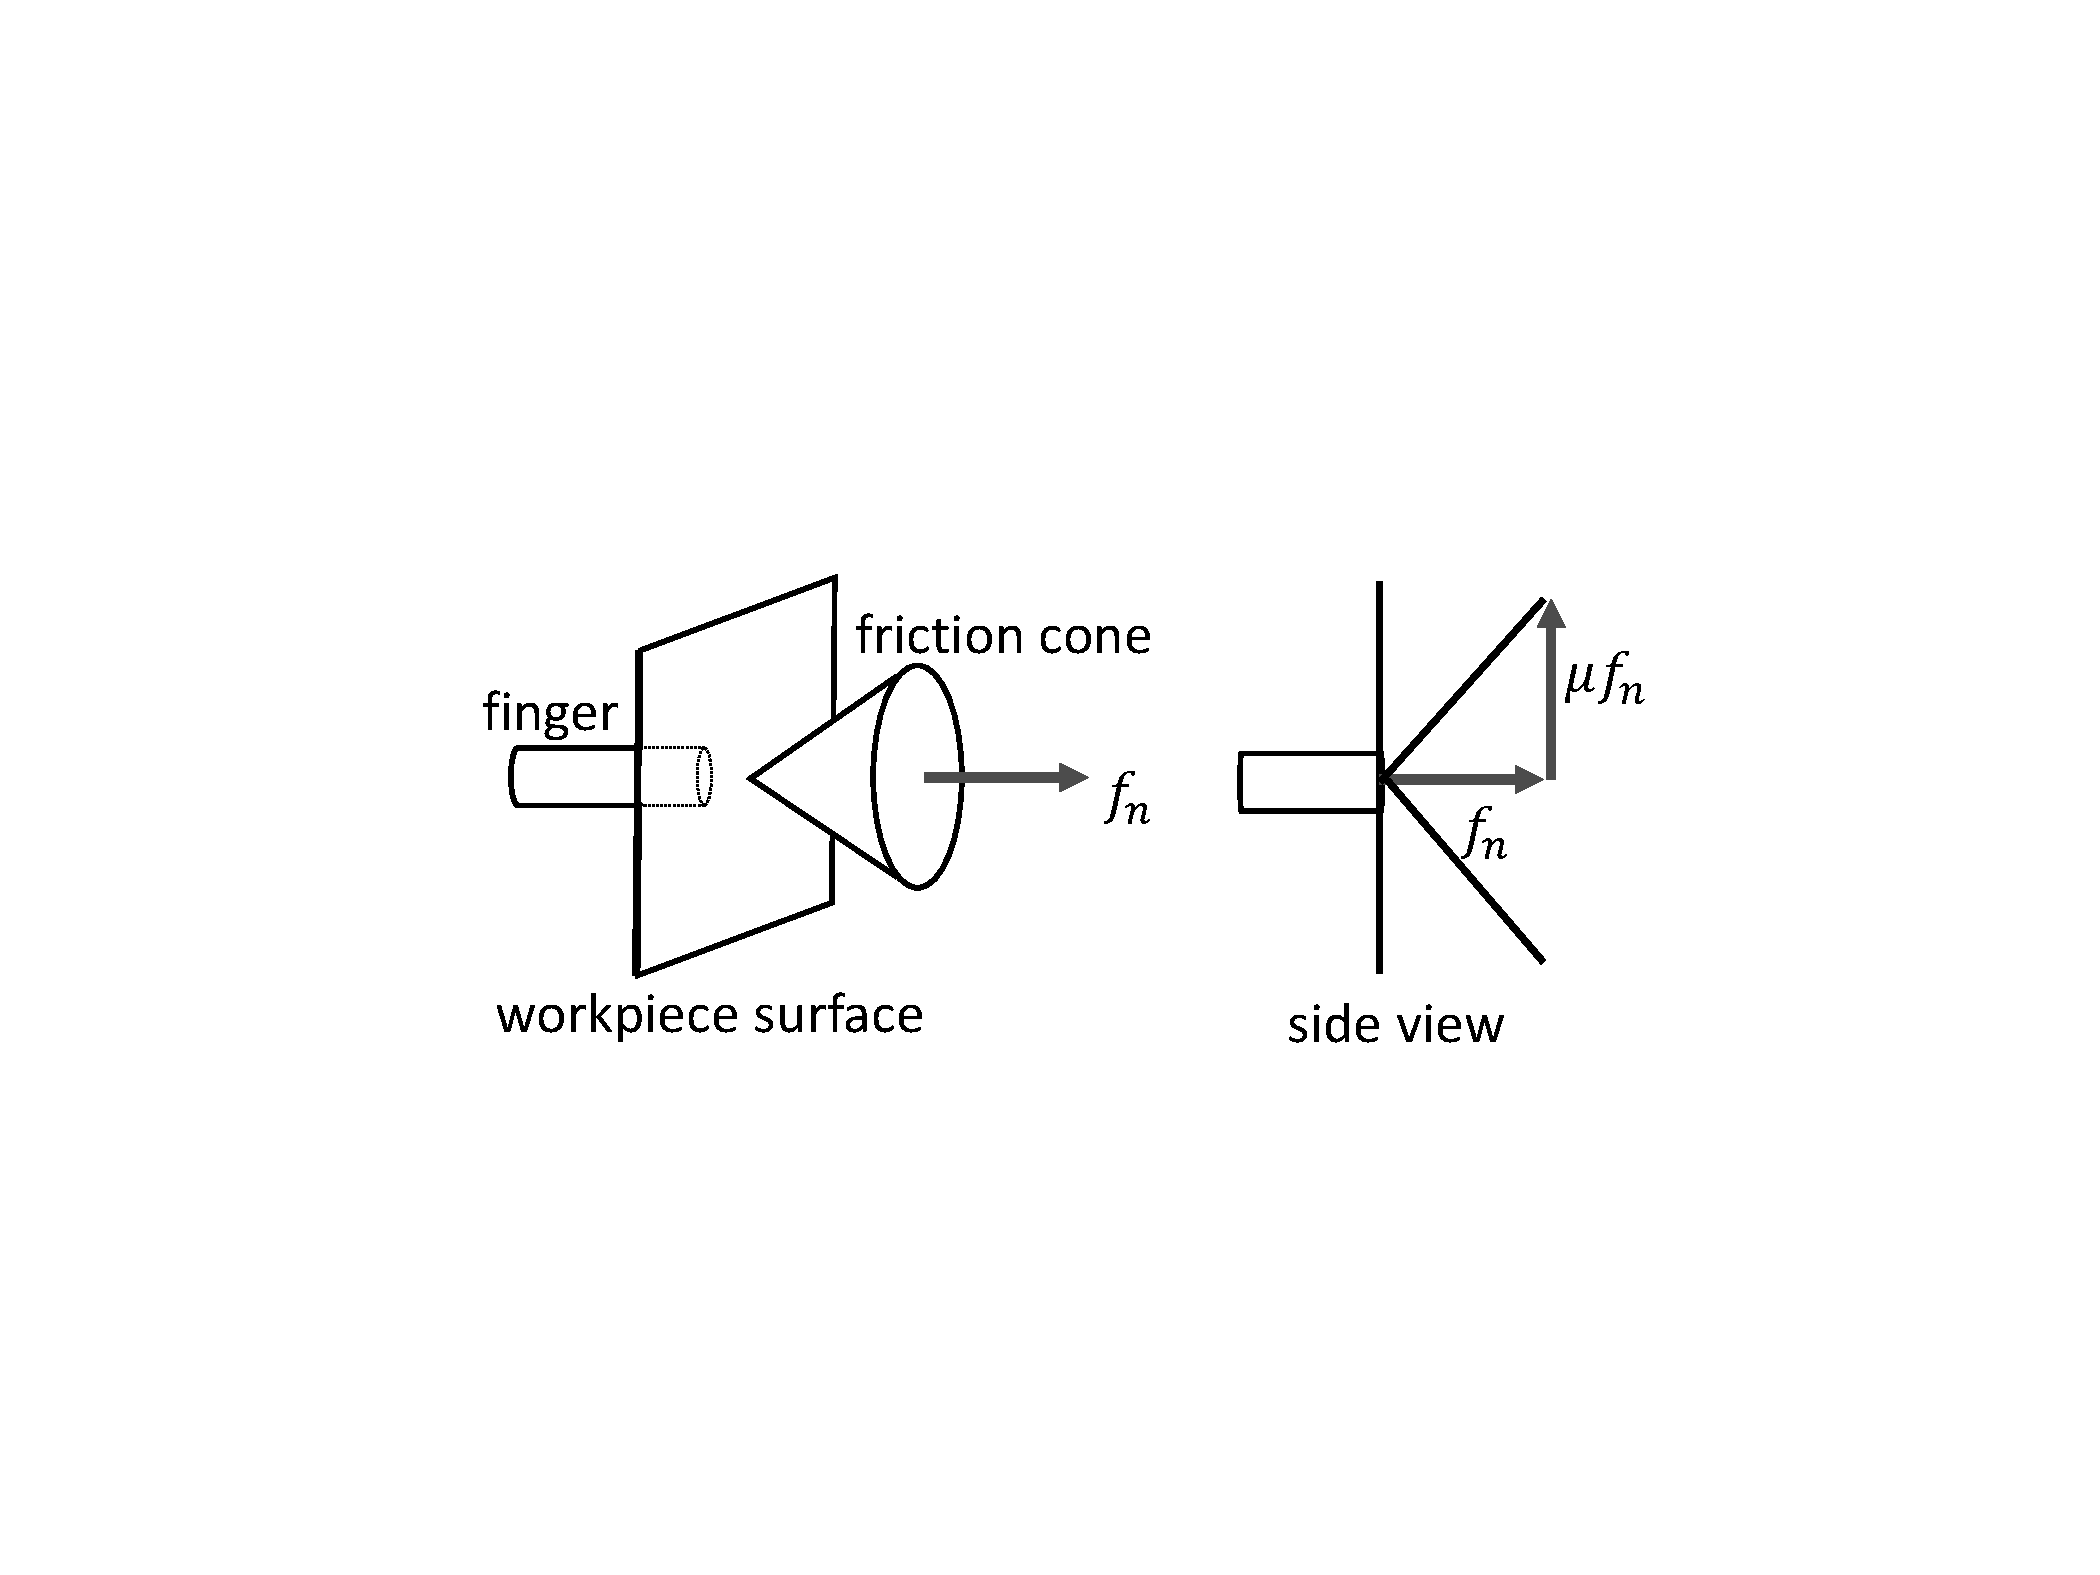
\includegraphics[trim={7cm 8cm 7cm 9cm},clip,width=1\linewidth,angle=0]{Cap2/Figuras/friction_contact.pdf}}
\centerline{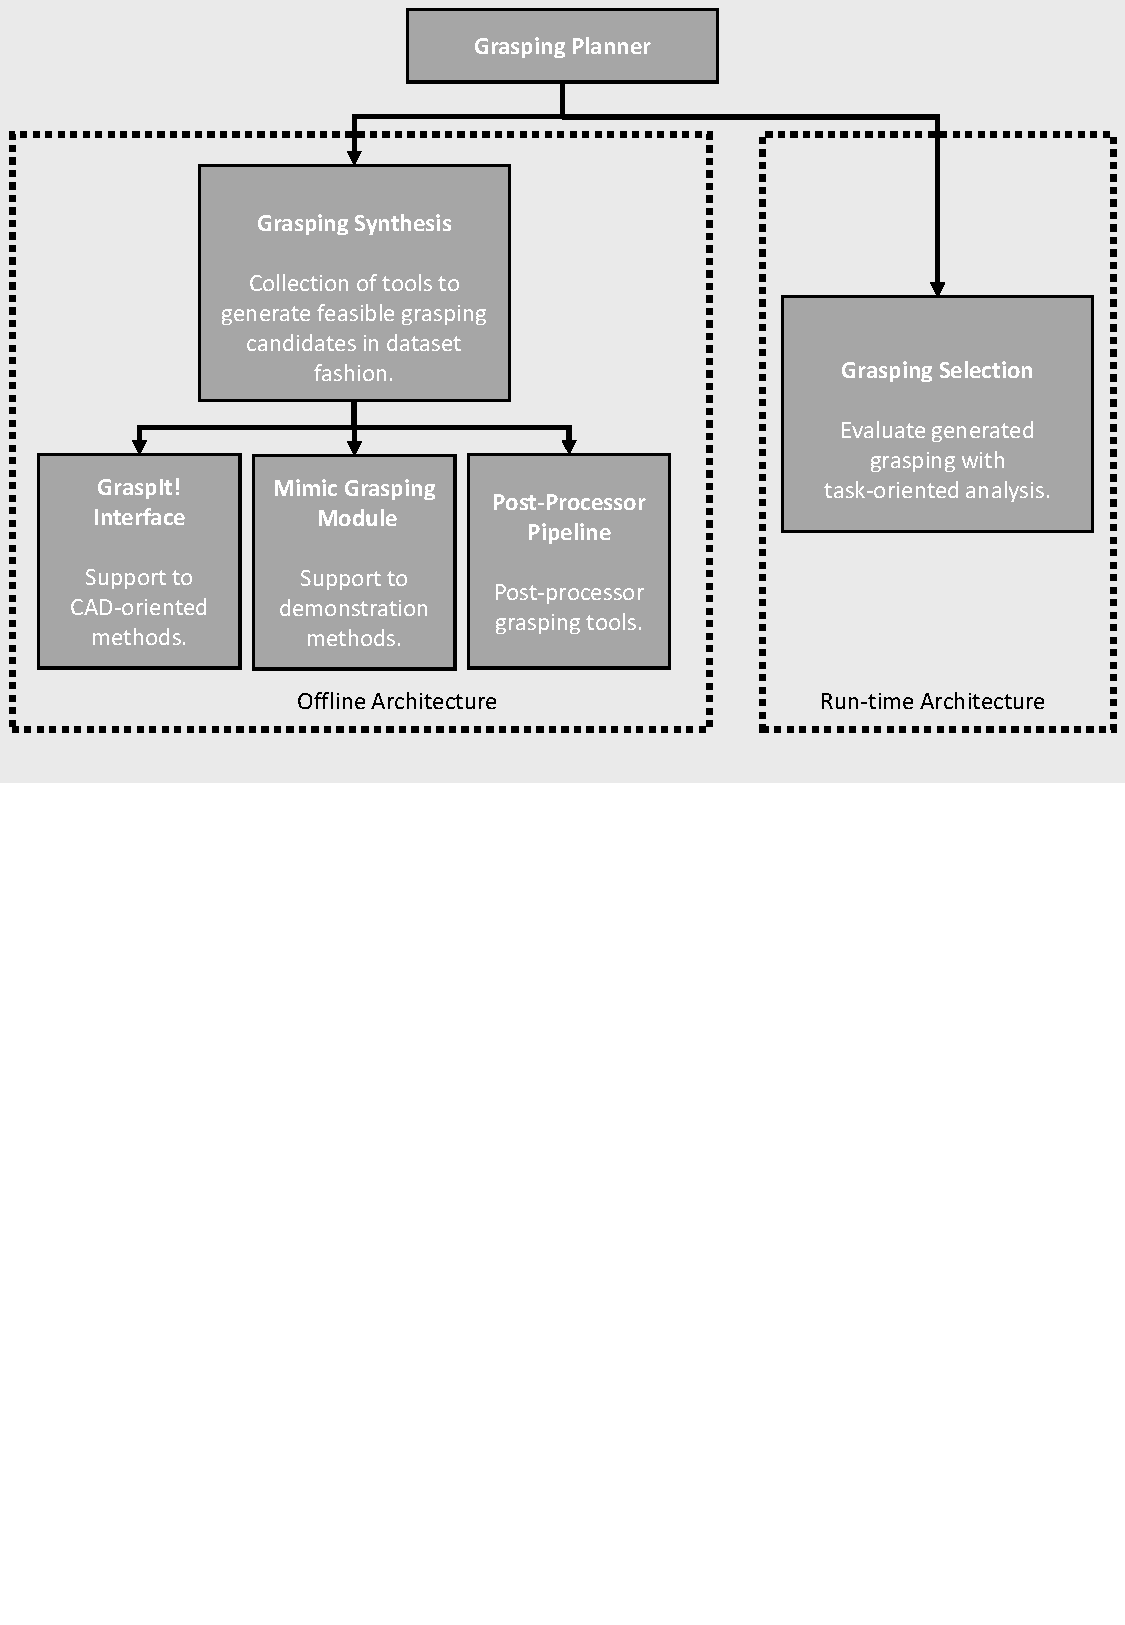
\includegraphics[trim={0cm 15cm 0cm 0cm},clip,width=0.95\linewidth,angle=0]{Cap4/Figuras/grasping_framework.pdf}}
\end{tcolorbox}
\caption{Proposed modular grasping architecture.}
\label{fig:grasping_framework_code}
\end{figure}

\section{Grasping Synthesis}
\label{cap4:modular_grasping_architecture:sec:grasping_synthesis}

The ``Grasping Synthesis'' is a set of tools responsible, in a pipeline fashion, for generating and handling the grasping poses dataset. This pipeline is an offline step, i.e., it runs outside the robot system in a setup phase. The dataset is created as a set of hypothetical grasping pose candidates which are hierarchically structured in a YAML file format. The proposed dataset standard is detailed discussed in Section~\ref{cap4:modular_grasping_architecture:sec:grasping_dataset}.

Currently three main components constitutes the grasping synthesis: the ``GraspIt!'' Interface (Section~\ref{cap4:modular_grasping_architecture:sec:grasping_synthesis:subsec:graspit}), the Mimic Grasping Module (Section~\ref{cap4:modular_grasping_architecture:sec:grasping_synthesis:subsec:mimic_grasping}) and the Post-Processor Pipeline (Section~\ref{cap4:modular_grasping_architecture:sec:grasping_synthesis:subsec:post_processor}). 

\subsection{Grasping Dataset Standard}
\label{cap4:modular_grasping_architecture:sec:grasping_dataset}

A grasping candidate, also referred as candidate, is defined by its pose over an object geometry. Besides this fundamental characteristic, others should be defined according to gripper in usage. Therefore, a structured grasping candidate dataset is proposed. This is a standard which allows new increments according to new future grippers addition.

The candidates are specified by an YAML descriptor (Snippet \ref{code:candidates_dataset}) and they are sequentially located in a YAML configuration file. %This dataset file can be loaded in the ROS parameter server afterwards. 

%\begin{minipage}{1\textwidth}
\begin{snippet}[h!]
	\centering
	\resizebox{0.75\textwidth}{!}{%	
	\begin{tcolorbox}
	\lstinputlisting[%caption= The candidate dataset descriptor example.,
	                  abovecaptionskip=3pt,
	                  captionpos=b,
	                  style=yaml,
	                  linerange={0-18},
	                  firstnumber=25,
	                  %label=code:candidates_dataset
	                  ]
	                  {Cap4/codes/candidates_dataset.yaml}
	\end{tcolorbox}
	}
	\caption{The candidate dataset descriptor example.}
	\label{code:candidates_dataset}
\end{snippet}
%\end{minipage}

The candidates are unique for gripper-object, therefore there exists one datatset per active pair, and they are named as ``candidate$\_$id'', where id is a integer that defines the order into datatset. 

Since the dataset standard is created focused on being applied to a modular grasping pipeline, which allows the integration of different methodologies, the first parameter, ``method/type'' is an integer that defines which synthesis method builds the candidate. Based on the configurable premiss, the supported gripper is defined by an integer code by ``gripper/type'' parameter followed by the ``gripper/parameters'' array. This dynamic size array is related to more complex grippers such as the adaptive RobotiQ models~\cite{robotiq_grippers} that grant more joints control. The ``gripper/type'' parameter define how to read this array, e.g for gripper type 0 (RobotiQ 2f84) and 1 (RobotiQ 2f140) the sequence is: force [N], velocity[m/s], pre-grasp-width [m], grasp-width [m], grasp-release-width [m], grasping model. On the other hand, grippers such as HGPC16A (Figure~\ref{fig:mimic_grippers_supported}) have an empty array since the control is performed only by the ON/OFF state. Any new model added to architecture should have this array described and defined. The ``gripper/DOFs'' is also a dynamic size array with fingers' joints \acp{DOF} value. Since the grasping candidate could be defined by the \textit{eingengrasp} (Section~\ref{sec:sim_ann}) or by the individual finger joint state, the ``method/type" defines how to extract this information from the array. Another important parameter to define this array is the ``gripper/type''. 

The position is given in meters followed by the orientation in quaternion w.r.t. ``parent$\_$frame$\_$id'' reference frame which if it is not declared, is considered the object reference;


%The others descriptor parameters are defined below:

%\begin{itemize_jp}
%    \item \textbf{method/type:} an integer that defines which synthesis method build the candidate. %Supported values in current thesis are: 0$\_$MANUAL, 1-SANN$\_$MULTIFINGERED, 2-SANN$\_$SUCTION. 3-MIMIC$\_$GRASPING;
%    \item \textbf{gripper/type:} an integer that defines the gripper type. %Supported values in current thesis are: 0-ROBOTIQ$\_$2F$\_$85, 1-ROBOTIQ$\_$2F$\_$140, 2-ROBOTIQ$\_$3F, 3-SUCTION, 4-FESTO$\_$2F$\_$HGPC$\_$16$\_$A, 5-SCHMALZ$\_$SINGLE$\_$RECT$\_$SUCTION;
%    \item \textbf{gripper/parameters:} a dynamic size array with specific gripper's parameters. Typically these parameters are related to more complex grippers such as Robotiq models~\cite{robotiq_grippers}. The ``gripper/type'' parameter define how to read this array, e.g for gripper type 0 (robotiq 2f84) and 1 (robotiq 2f140) the sequence is: force [N], velocity[m/s], pre-grasp-width [m], grasp-width [m], grasp-release-width [m], grasping model. On the other hand, grippers such as HGPC16A (Figure~\ref{fig:mimic_grippers_supported}) have a empty array since the control is performed only by ON/OFF state. Any new model added into architecture should have this array described and defined;
%    \item \textbf{gripper/DOFs:} a dynamic size array with fingers' joints \acp{DOF} value. Since the grasping candidate could be defined by the eingengrasp (Section~\ref{ap:sim_ann}) or by the individual finger joint state, the ``method/type" defines how to extract this information from the array. Another important parameter to define this array is the ``gripper/type''; 
%    \item \textbf{parent$\_$frame$\_$id:} reference frame in which the candidate is defined. If it is not declared, it is considered the object reference;
%    \item \textbf{position:} position w.r.t. parent frame id, in meters.
%    \item \textbf{orientation:} orientation w.r.t. parent frame id, in quaternion.
%\end{itemize_jp}

\subsection{``GraspIt" Interface}
\label{cap4:modular_grasping_architecture:sec:grasping_synthesis:subsec:graspit}

The ``GraspIt!" interface is responsible to generate grasping candidates based on CAD modelling by using the ``GraspIt!" API and simulator (Figure~\ref{fig:graspit_manual_feeder_workflow}), in association with \ac{ROS} framework. This simulator was first proposed by~\cite{miller2004graspit} and is widely used in academic community to multi-fingered grasping analysis (Section~\ref{sec:multifingered_grasping}) using CAD interaction in virtual environment. The grippers are structured in XML format (besides the 3D model, the \ac{ICR} and the \textit{eigengrasps}, Section~\ref{sec:sim_ann}, are also defined). The objects are included by using a Polygon File Format (extension ``.ply'').

\begin{figure}[h!]
	\resizebox{1\textwidth}{!}{%
		\begin{tcolorbox}
			\centerline{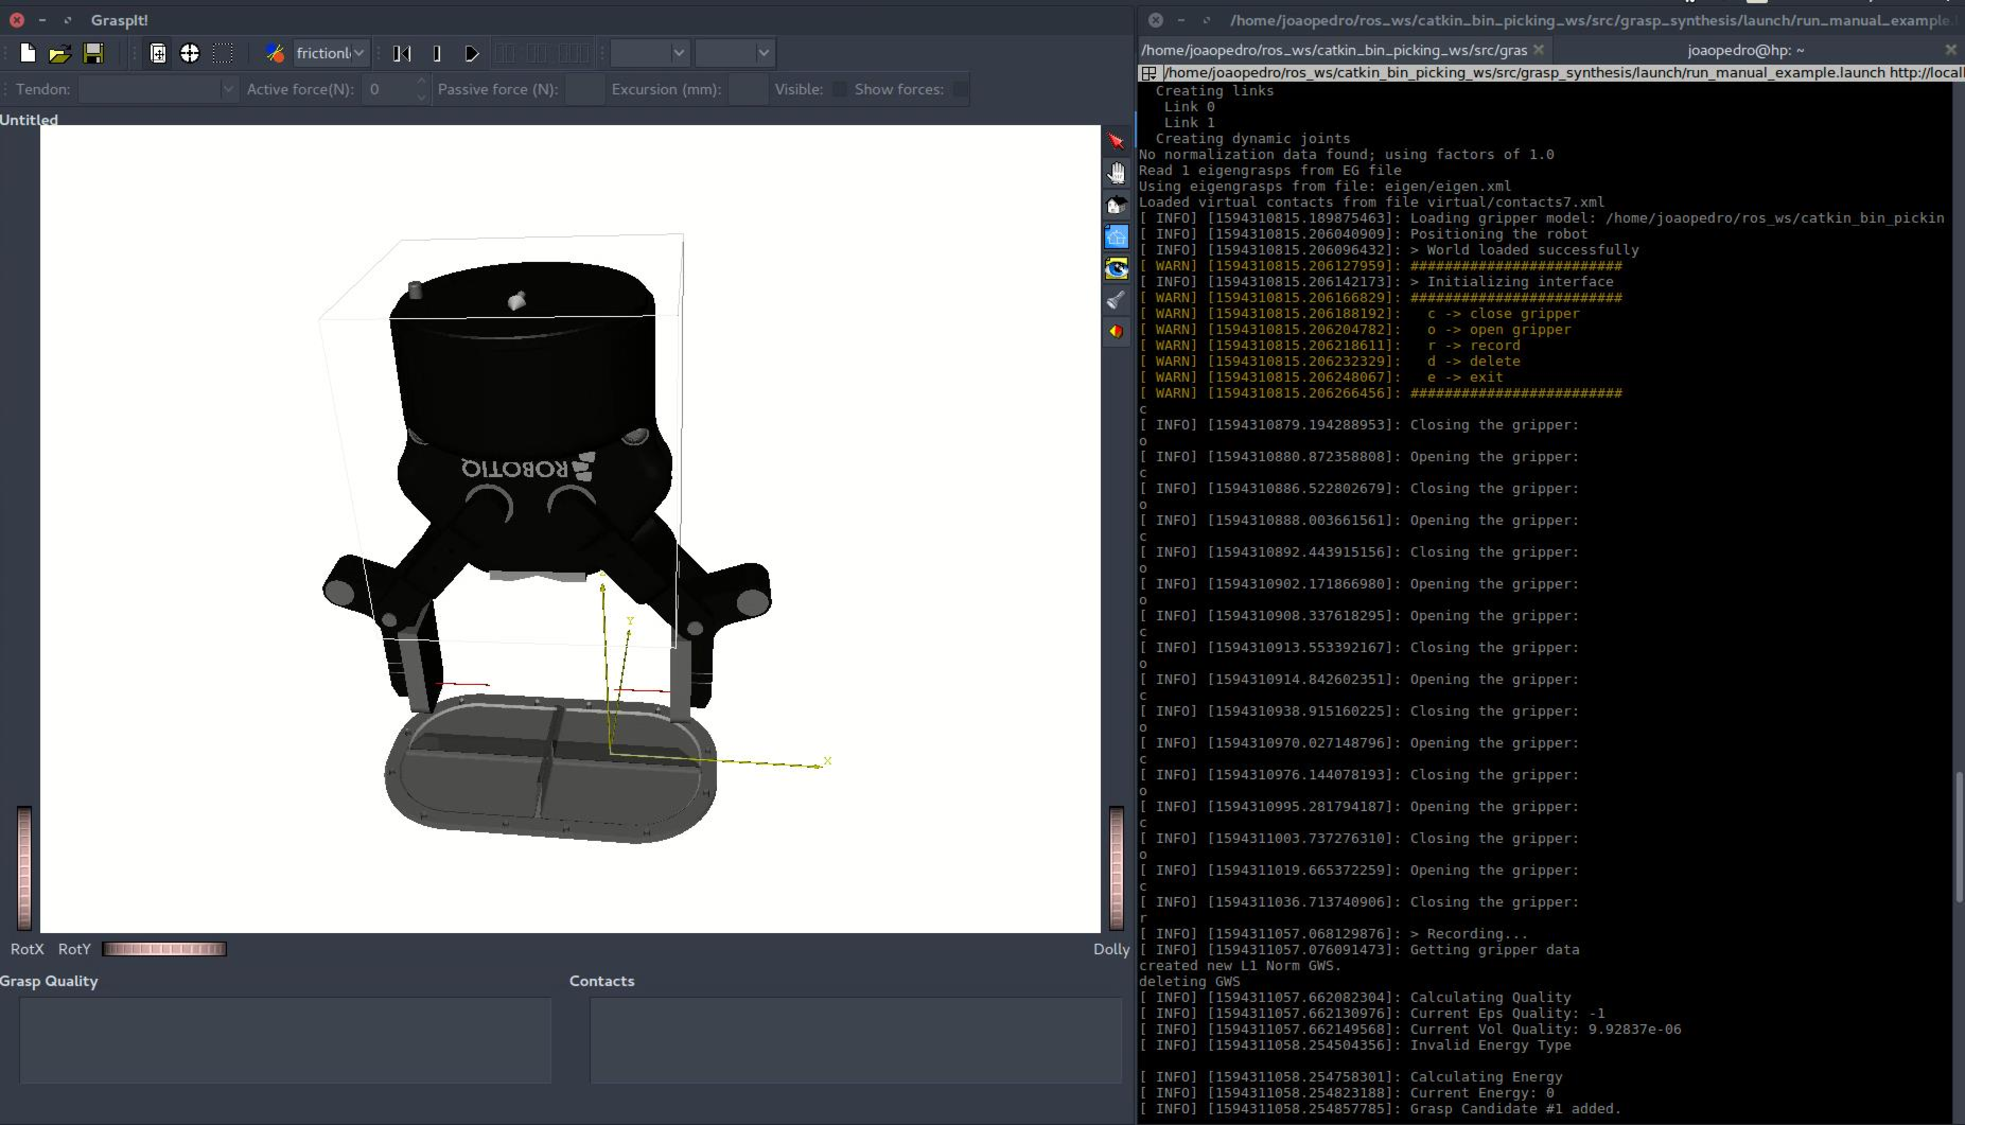
\includegraphics[trim={0cm 0cm 1cm 0cm},clip,width=1\linewidth,angle=0]{Cap4/Figuras/graspit_manual_support.pdf}}
		\end{tcolorbox}
		\caption{``GraspIt!" interface and the implemented manual feeder.}
		\label{fig:graspit_manual_feeder_workflow}
	}%end resize box
\end{figure}

The Figure~\ref{fig:grasping_graspit_module_workflow} presents the ``GraspIt" interface pipeline workflow.

\begin{figure}[h!]
\resizebox{1\textwidth}{!}{%
\begin{tcolorbox}
\centerline{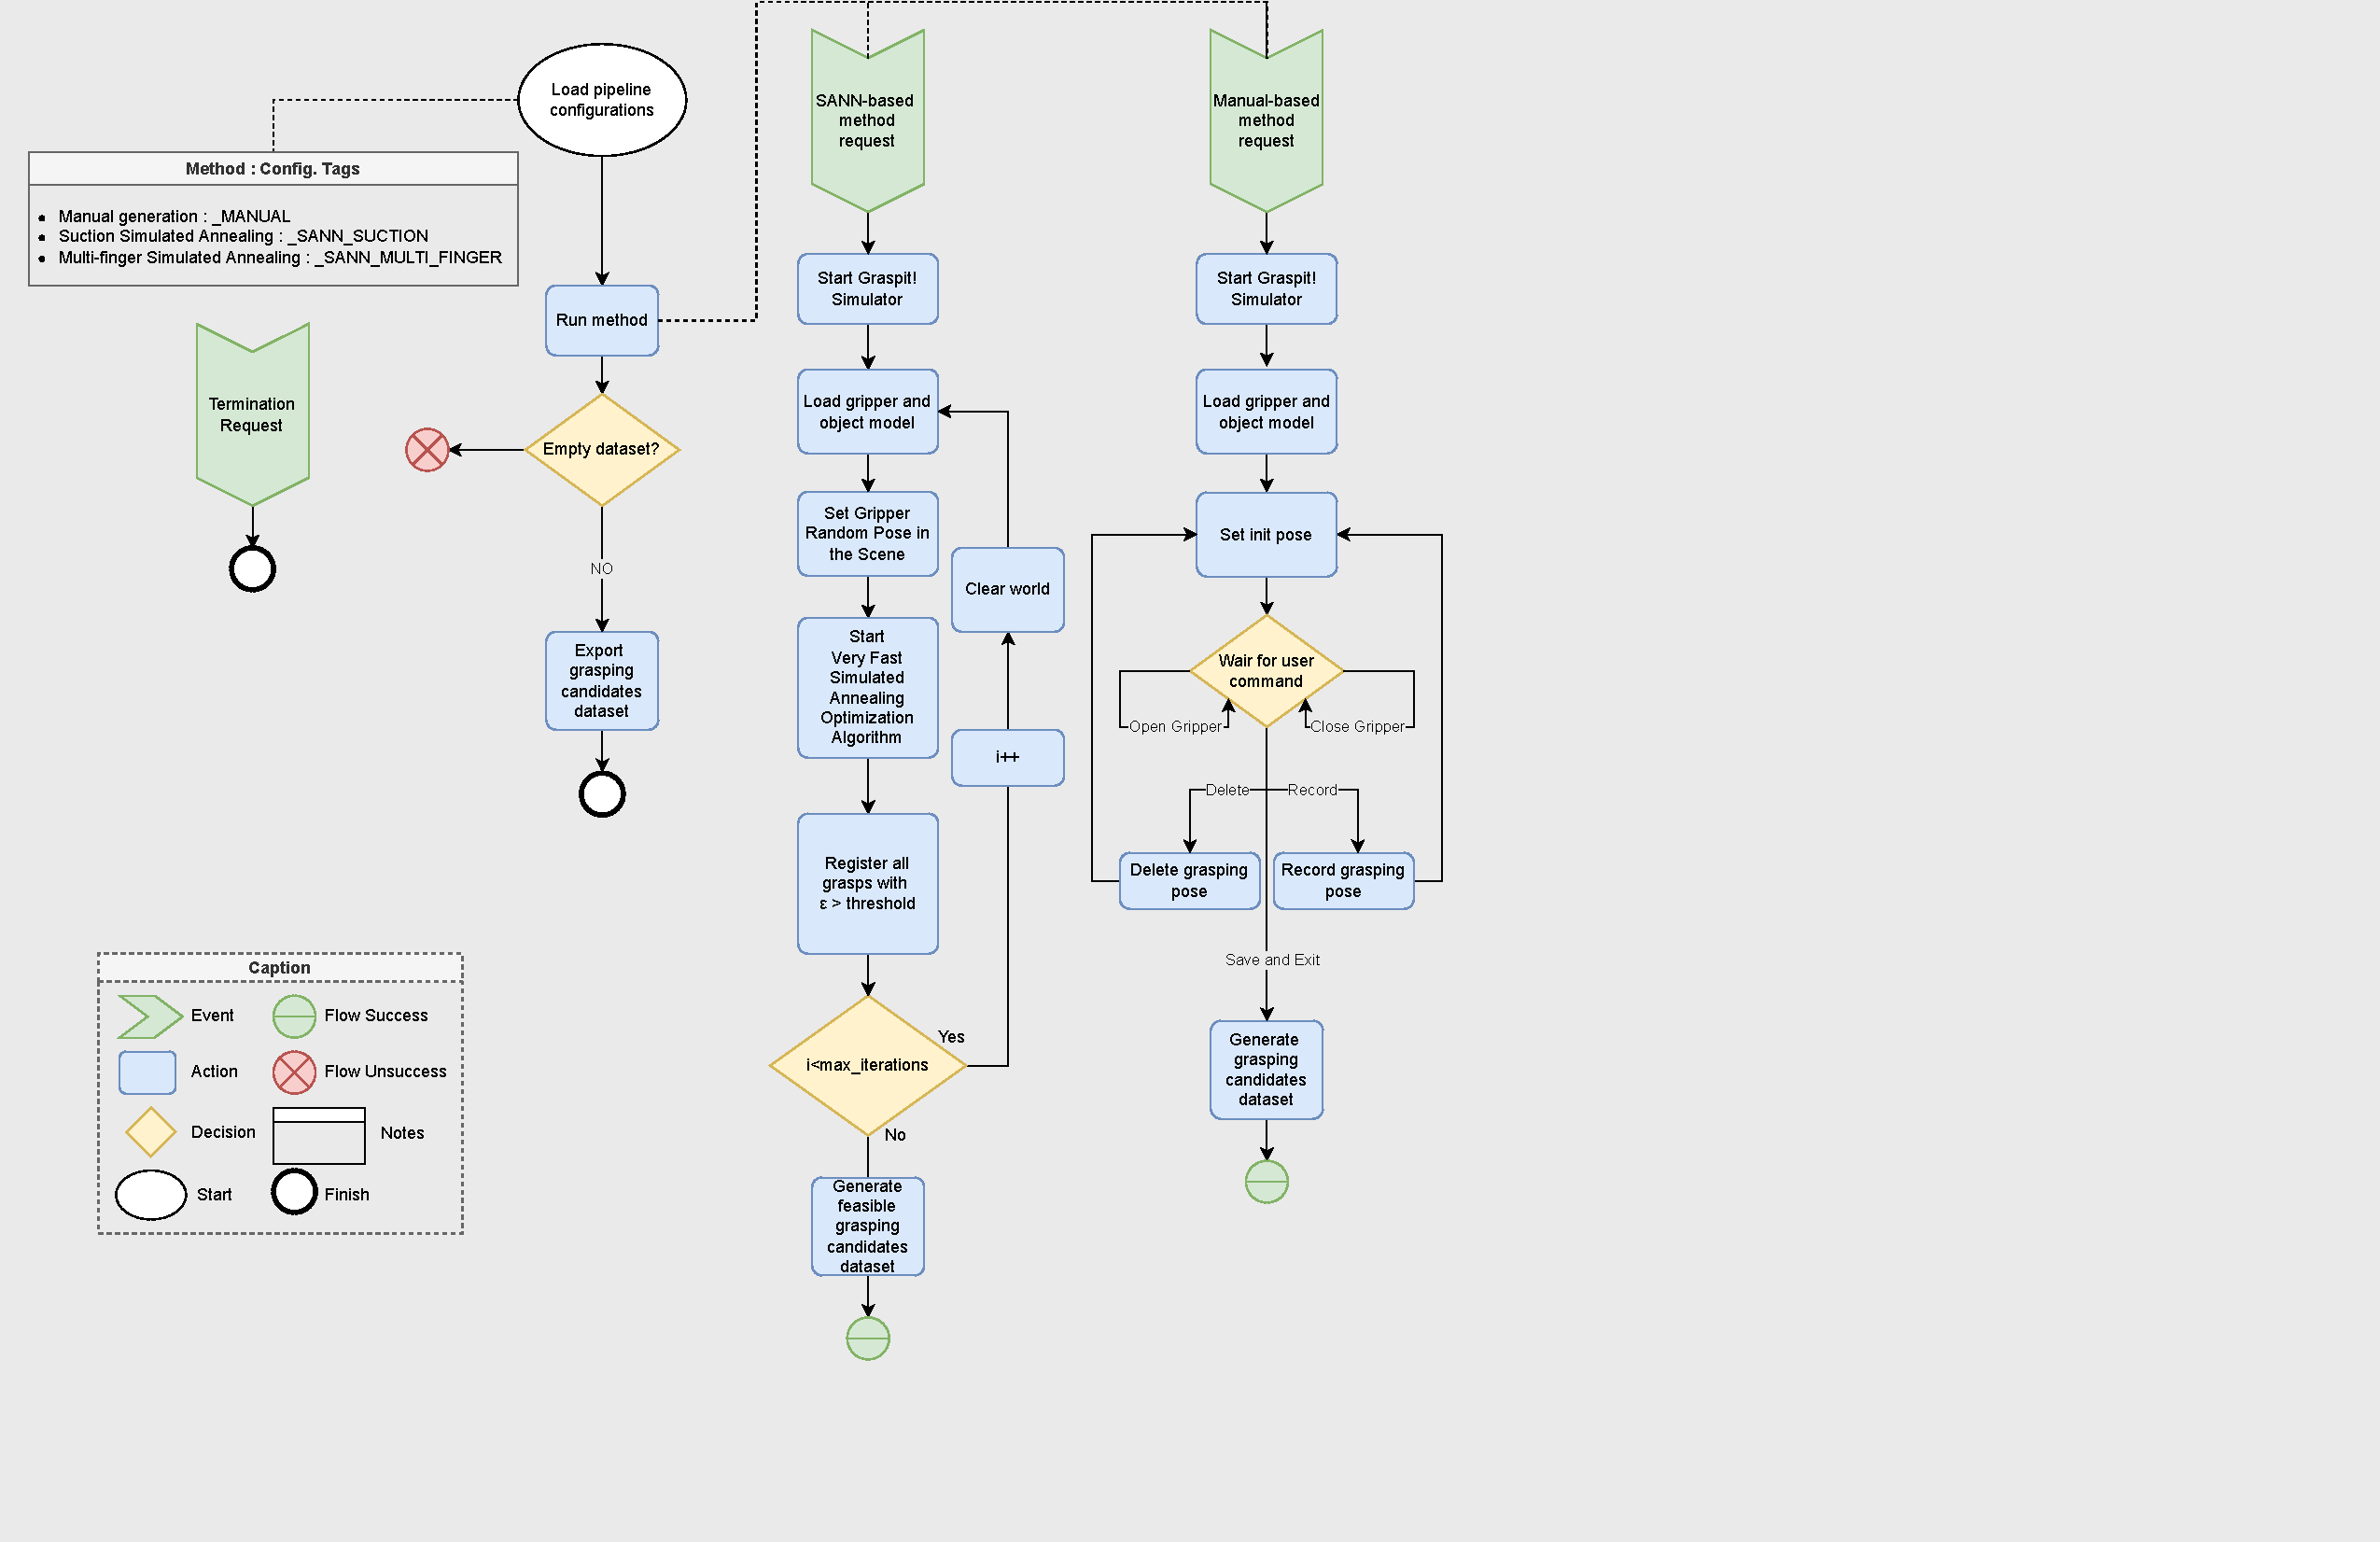
\includegraphics[trim={0.5cm 3cm 17cm 0cm},clip,width=1\linewidth,angle=0]{Cap4/Figuras/flowchart_graspit_module.pdf}}
\end{tcolorbox}
\caption{``GraspIt!" interface pipeline workflow. }
\label{fig:grasping_graspit_module_workflow}
}%end resize box
\end{figure}

The implemented methods are discussed into Sections~\ref{cap4:modular_grasping_architecture:sec:grasping_synthesis:subsec:graspit:subsubsec:manual} and~\ref{cap4:modular_grasping_architecture:sec:grasping_synthesis:subsec:graspit:subsubsec:sann}. The interface is based on C++ polymorphic classes which allows new heuristics design and also incorporate new future ``GraspIt!" functionalities. 

\subsubsection{Manual Feeder}
\label{cap4:modular_grasping_architecture:sec:grasping_synthesis:subsec:graspit:subsubsec:manual}

The manual feeder allows the user to define grasping postures by interacting with ``GraspIt!" 3D environment, Figure~\ref{fig:graspit_manual_feeder_workflow}. This feeder automatic call and configure the ``GraspIt!" virtual interface. It also call a menu, which allows the operator to store, delete, manipulate the gripper and generate the grasping dataset based on the thesis' proposed standard (Section~\ref{cap4:modular_grasping_architecture:sec:grasping_dataset}). The YAML descriptor is defined in Snippet~\ref{code:manual_feeder}. %and its parameters is presented below:

%\begin{minipage}{1\textwidth}
\begin{snippet}[h!]
	\centering
	\resizebox{0.75\textwidth}{!}{%
	\begin{tcolorbox}
	 \lstinputlisting[%caption= The ``GraspIt!" manual descriptor example.,
	                  abovecaptionskip=3pt,
	                  captionpos=b,
	                  style=yaml,
	                  linerange={0-14},
	                  firstnumber=25,
	                  %label=code:manual_feeder
	                  ]
	                  {Cap4/codes/manual_feeder.yaml}
	\end{tcolorbox}
	}
	\caption{The ``GraspIt!" manual descriptor example.}
	\label{code:manual_feeder}
\end{snippet}
%\end{minipage}

%\begin{itemize_jp}
%    \item \textbf{path/gripper$\_$models$\_$file$\_$path:} path to locate the gripper XML model;
%    \item \textbf{path/object$\_$models$\_$file$\_$path:} path to locate the object ``.ply" model;
%    \item \textbf{gripper$\_$file$\_$name:} gripper XML file name;
%    \item \textbf{object$\_$file$\_$name:} object polygon file format name;
%    \item \textbf{config$\_$grasps$\_$parameters/gripper$\_$id:} gripper ID code;
%    %\item \textbf{config$\_$grasps$\_$parameters/grasp$\_$model: } 
%    %\item \textbf{config$\_$grasps$\_$parameters/velocity: } approach velocity. 
%    %\item \textbf{config$\_$grasps$\_$parameters/force: }
%    \item \textbf{config$\_$grasps$\_$parameters/approach$\_$width$\_$multiplier:} the multiplier to define the grasping width in approach procedure. This value is applied over the grasping candidate width;
%    \item \textbf{config$\_$grasps$\_$parameters/release$\_$width$\_$multiplier:} the multiplier to define the grasping width in release procedure. This value is applied over the grasping candidate width;
%    \item \textbf{config$\_$grasps$\_$parameters/min$\_$width$\_$threshold:} minimum width to consider in grasping procedure. Some grippers have flexible finger that need to be considered.
%\end{itemize_jp}

The gripper model path and name are defined in ``$path/gripper$\_$models$\_$file$\_$path$'' and ``$gripper$\_$file$\_$name$'', respectively. It should respect the ``GraspIt!'' XML description standard with its \ac{ICP}, \textit{eigengrasp} and Denavit-Hatenberg definitions. Focused on pipeline configurability, the gripper code ID is defined in ``$config$\_$grasps$\_$parameters/gripper$\_$id$'' and it is mapped according to the pipeline implementation. Other custom parameters are the ``$approach$\_$width$\_$multiplier$'' and ``$release$\_$width$\_$multiplier$'' which are multiplication factors to define the grasping width in the approach and release procedure. These values are applied over the grasping candidate width and it is important to avoid possible collision between the fingers during the grasping approaching and placing approaching movement.  The ``$config$\_$grasps$\_$parameters/min$\_$width$\_$threshold$'' is the minimum width to consider in grasping procedure. Some grippers have a flexible finger that needs to be considered.
In the end, the polygon file format of the object model should be defined by ``$path/object$\_$models$\_$file$\_$path$'' and ``$object$\_$file$\_$name$''.


\subsubsection{\acl{SANN} based Feeder}
\label{cap4:modular_grasping_architecture:sec:grasping_synthesis:subsec:graspit:subsubsec:sann}

The ``Graspit!" has support to grasping automatic generation by using the Very Fast \acl{SANN} optimisation algorithm. For a detailed explanation referrer to Section~\ref{sec:sim_ann}. This functionality is also incorporated into the core pipeline by the YAML descriptor presented in Snippet~\ref{code:multifingered_sann}. Besides the multi-fingered approach (Section~\ref{sec:multifingered_grasping}), a descriptor to suction grippers is designed considering that good suction grasping is directly related to well define contact point Snippet~\ref{code:suction_sann}.

%\begin{minipage}{1\textwidth}
\begin{snippet}[h!]
\centering
\resizebox{0.75\textwidth}{!}{%
\begin{tcolorbox}
 \lstinputlisting[
                  %caption= The ``GraspIt!" multi-finger\ac{SANN} YAML descriptor example.,
                  abovecaptionskip=3pt,
                  captionpos=b,
                  style=yaml,
                  linerange={0-34},
                  firstnumber=25,
                  %label=code:multifingered_sann
                  ]
                  {Cap4/codes/multifingered_sann_feeder.yaml}
\end{tcolorbox}
}
\caption{The ``GraspIt!" multi-finger \ac{SANN} YAML descriptor example.}
\label{code:multifingered_sann}
\end{snippet}
%\end{minipage}


%\begin{minipage}{1\textwidth}
\begin{snippet}[h!]
\centering
\resizebox{0.75\textwidth}{!}{%
\begin{tcolorbox}
 \lstinputlisting[%caption= ``GraspIt!" suction \ac{SANN} YAML descriptor example.,
                  abovecaptionskip=3pt,
                  captionpos=b,
                  style=yaml,
                  linerange={0-34},
                  firstnumber=25,
                  %label=code:suction_sann
                  ]
                  {Cap4/codes/suction_sann_feeder.yaml}
\end{tcolorbox}
}
\caption{``GraspIt!" suction \ac{SANN} YAML descriptor example.}
\label{code:suction_sann}
\end{snippet}
%\end{minipage}

\begin{itemize_jp}
    \item \textbf{path/gripper$\_$models$\_$file$\_$path:} path to locate the gripper XML model;
    \item \textbf{path/object$\_$models$\_$file$\_$path:} path to locate the object ``.ply" model;
    \item \textbf{gripper$\_$file$\_$name:} gripper XML file name;
    \item \textbf{object$\_$file$\_$name:} object polygon file format name;
    \item \textbf{graspable$\_$body$\_$id:} defines which object in scene is the grasping focus;
    %\item \textbf{planner$\_$type$\_$:}
    \item \textbf{graspable$\_$body$\_$id:} defines which object in scene is the grasping focus;
    \item \textbf{action$\_$graspit$\_$interface$\_$server$\_$name:} since the ``GraspIt!" server is deployed as a \ac{ROS} action server~\cite{ros_action_lib}, its names should be specified;
    \item \textbf{action$\_$server$\_$timeout:} timeout to detect that the  ``GraspIt!" server is not running; 
    \item \textbf{iterations:} how many iterations the \ac{SANN} will be executed (Figure~\ref{fig:grasping_synthesis_core});
    \item \textbf{energy$\_$threshold:} convergence optimisation threshold; 
    %\item \textbf{impose$\_$force$\_$closure$\_$to$\_$near$\_$grasps:} in each \ac{SANN} iterations several grasping candidates are generated. Some grasping candidates are discarded during the optimisation procedure since does not respect the \ac{ICR} approximation criteria. However  
    %\item \textbf{epsilon$\_$threshold:}
    \item \textbf{sim$\_$annealing/max$\_$steps:} maximum steps of one \ac{SANN} iteration;
    \item \textbf{sim$\_$annealing/feedback$\_$num$\_$steps:} allow visual update of optimisation process;
    \item \textbf{sim$\_$annealing/set$\_$custom$\_$params:} set custom params;
    \item \textbf{sim$\_$annealing/YC:} annealing constant for neighbor generation schedule;
    \item \textbf{sim$\_$annealing/HC:} annealing constant for error acceptance schedule;
    \item \textbf{sim$\_$annealing/YDIMS:} number of dimensions for neighbor generation schedule;
    \item \textbf{sim$\_$annealing/HDIMS:} number of dimensions for error acceptance schedule;
    \item \textbf{sim$\_$annealing/NBR$\_$ADJ:} adjust factor for neighbor generation schedule
    \item \textbf{sim$\_$annealing/ERR$\_$ADJ:} adjust raw errors reported by states to be in the relevant range of the annealing schedule;
    \item \textbf{sim$\_$annealing/DEF$\_$K0:} starting step;
    \item \textbf{sim$\_$annealing/DEF$\_$T0:} starting temperature;
    \item \textbf{config$\_$grasps$\_$parameters/gripper$\_$id:} gripper ID code;
    %\item \textbf{config$\_$grasps$\_$parameters/grasp$\_$model: } 
    %\item \textbf{config$\_$grasps$\_$parameters/velocity: } approach velocity. 
    %\item \textbf{config$\_$grasps$\_$parameters/force: }
    \item \textbf{config$\_$grasps$\_$parameters/approach$\_$width$\_$multiplier:} the multiplier to define the grasping width in approach procedure. This value is applied over the grasping candidate width;
    \item \textbf{config$\_$grasps$\_$parameters/release$\_$width$\_$multiplier:} the multiplier to define the grasping width in release procedure. This value is applied over the grasping candidate width;
    \item \textbf{config$\_$grasps$\_$parameters/min$\_$width$\_$threshold:} minimum width to consider in grasping procedure. Some grippers have flexible finger that need to be considered.
\end{itemize_jp}

\subsection{Mimic Grasping Module}
\label{cap4:modular_grasping_architecture:sec:grasping_synthesis:subsec:mimic_grasping}

The ``GraspIt!" interface (Section~\ref{cap4:modular_grasping_architecture:sec:grasping_synthesis:subsec:graspit}) generates grasping candidates based on CAD modeling interaction. This category could demand unnecessary effort if the gripper CAD modelling is not in disposition or if the gripper 3D design does not compensate for a simple grasping application with a reduced candidate number. Therefore, human demonstration approaches could facilitate this deployment that allows less knowledgeable users to create a grasping representation.  

A grasping demonstration task could be defined as two localisation problems: the human manipulation detection and the graspable object pose estimation. Several techniques are proposed in current literature to deal with both issues~\cite{ferreira2016stereo,COSTA2016113,hu2022grasps}, in association or individually. Therefore a structured demonstration grasping module architecture could improve the capacity to deploy, test and evaluate different techniques (e.g. computer vision heuristics and machine learning-based) and hardware setups (e.g. sensor technologies and grippers structures), correctly adapting to different applications necessities.

In this regard, the present thesis proposes a mimic grasping architecture in the format of C++ API based on plugin management. The related plugins system is also developed as an C++ API. The plugin strategy is important since different techniques could be implemented as a dynamic library that is loaded in run-time into the mimic grasping architecture without the need to recompile the core pipeline. 

The plugin manager API provides metadata interface allowing the designing of plugins and the support to load this type of dynamic library into custom core applications, Figure~\ref{fig:plugin_system_management} elucidates the proposal.


\begin{figure}[h!]
\resizebox{1\textwidth}{!}{%
\begin{tcolorbox}
\centerline{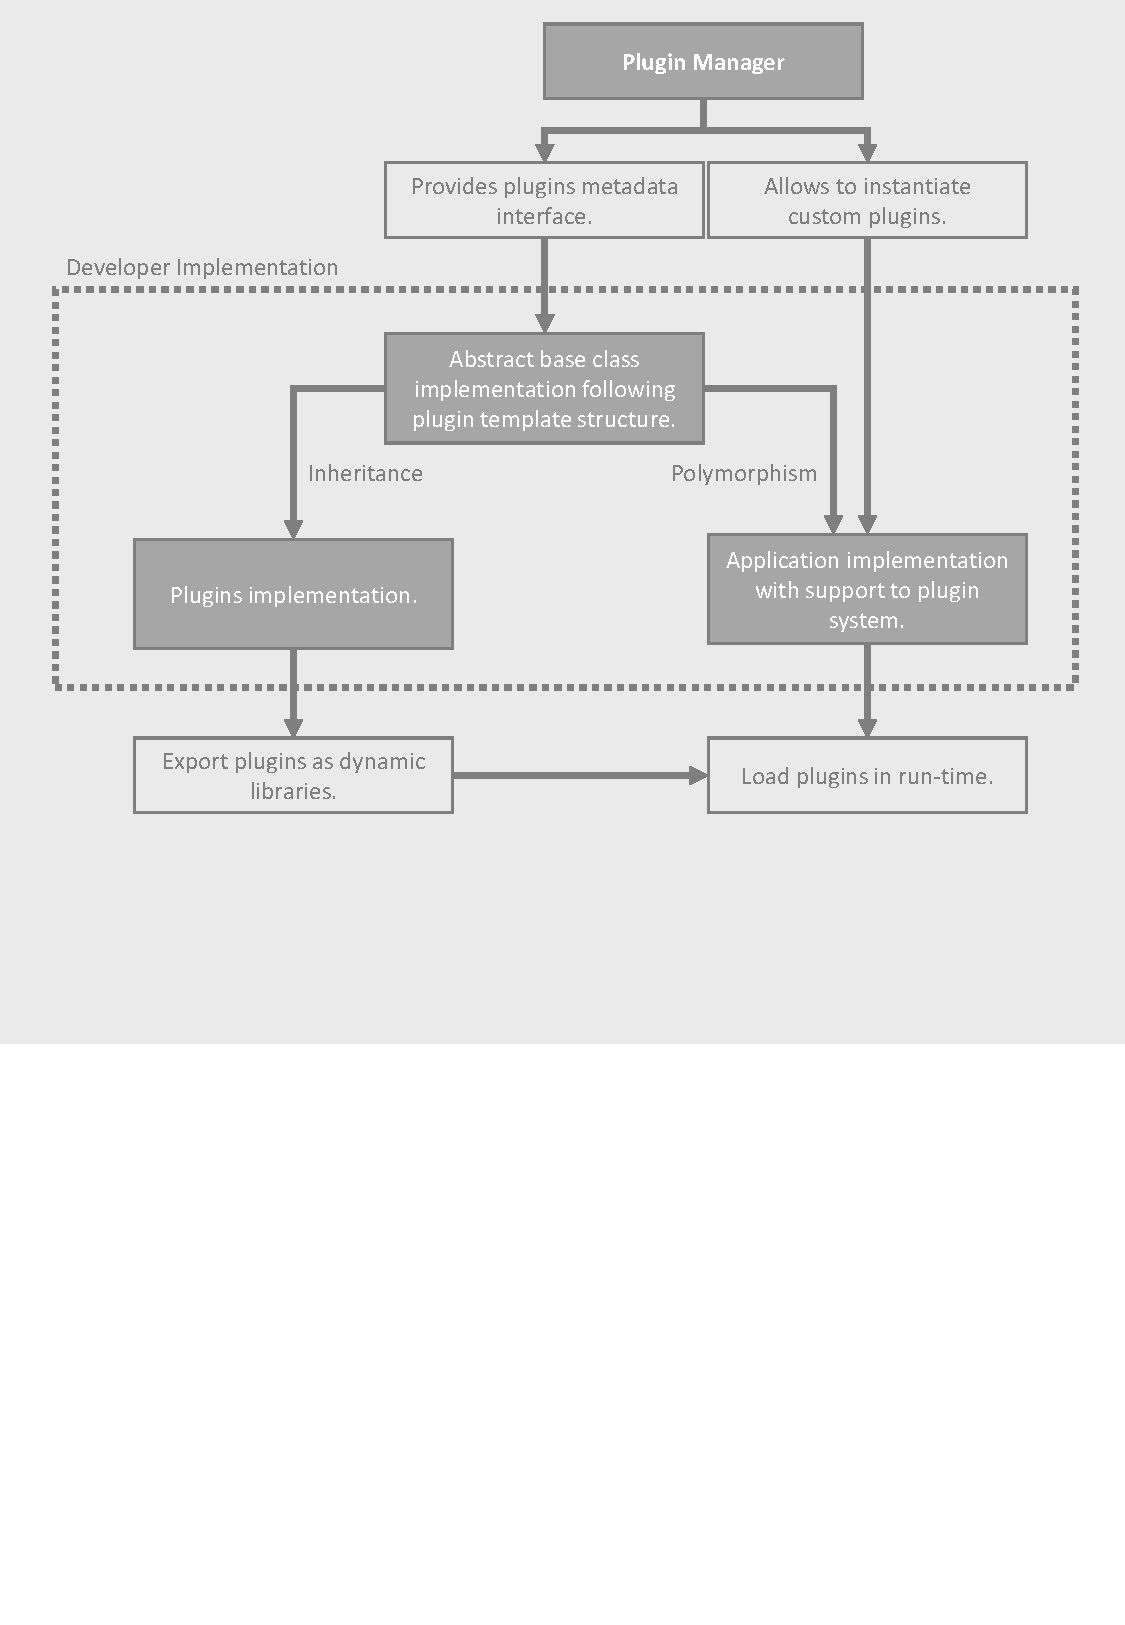
\includegraphics[trim={0cm 13cm 0cm 0cm},clip,width=1\linewidth,angle=0]{Cap4/Figuras/plugin_system_management.pdf}}
\end{tcolorbox}
\caption{Proposed plugin system management.}
\label{fig:plugin_system_management}
}
\end{figure}



The mimic grasping pipeline structured workflow is presented in Figure~\ref{fig:mimic_grasping_flowchart}. The mimic workflow concept considers that tools are necessary to define the human grasping, such as gloves or handler mechanisms, or at least a remote control technique that allows demonstrators requests while performing the demonstration. It is expected that the communication with the tool is performed by serial communication. In addition, it is considered that the two localisation methodologies, also called locators, are processed in sequence after the operator record request. 

Namely, this workflow starts by loading API general configurations, such as tool communication parameters and localisation methods definitions. The locators definition is composed by: the plugins definition such its dynamic library implementation file name and the configuration file by ``$plugin$\_$name$'' and ``$plugin$\_$config$\_$file$'', respectively.  The configuration file definition is necessary since the parameters are custom defined according to plugin implementation.

Typically, but not mandatory, plugins are client implementations since the localisation server could be loaded a part. Therefore the pipeline need to bring up these outer systems by running a user defined script (or a simple command), caller executor. At end, a shutdown scripts (or command), called terminator, is expected to turn off these systems. These commands or files are defined by setting the 
``$executor$\_$cmd$'' and ``$terminator$\_$cmd$'' parameters.

\begin{figure}[h!]
\resizebox{1\textwidth}{!}{%
\begin{tcolorbox}
\centerline{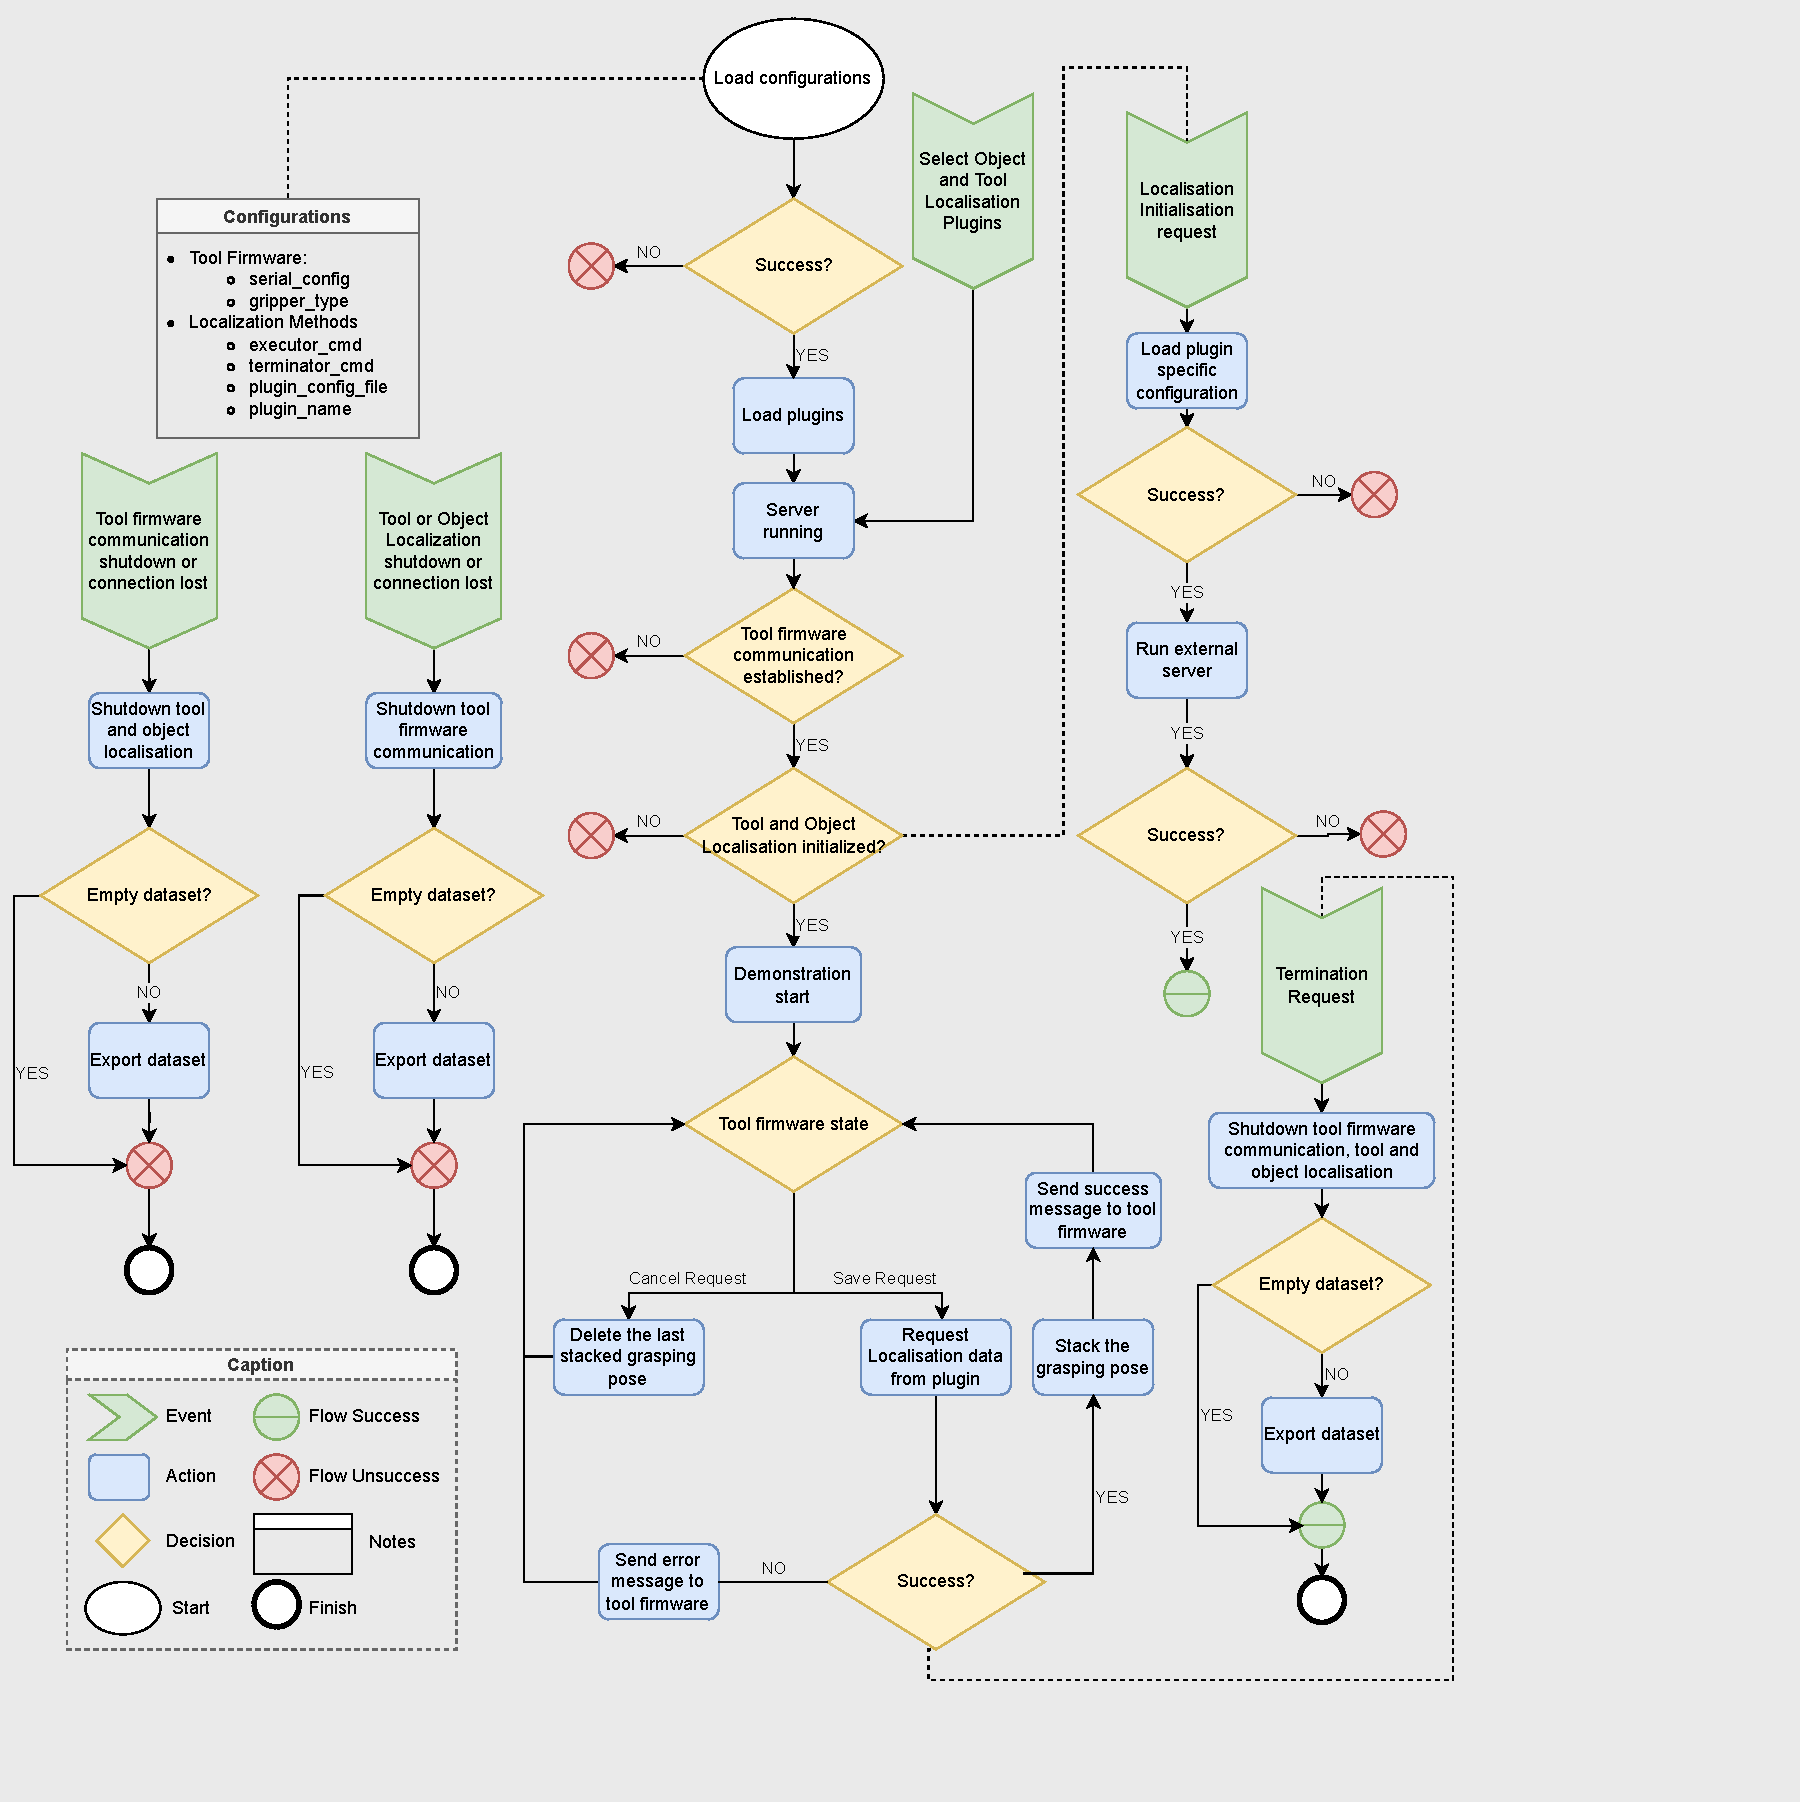
\includegraphics[trim={0cm 2cm 5.5cm 0cm},clip,width=1\linewidth,angle=0]{Cap4/Figuras/mimic_grasping_api_flowchart.pdf}}
\end{tcolorbox}
\caption{Proposed modular mimic grasping architecture.}
\label{fig:mimic_grasping_flowchart}
}
\end{figure}

%\begin{itemize_jp}
%    \item \textbf{plugin$\_$name:} the plugin dynamic library implementation file name;
%    \item \textbf{plugin$\_$config$\_$file:} the plugin dynamic library configuration file name. This is necessary since the parameters are custom defined according to plugin implementation;
%    \item \textbf{executor$\_$cmd and terminator$\_$cmd: } typically, but not mandatory, plugins are client implementations since the localisation server could be loaded a part. Therefore the pipeline need to bring up these outer systems by running a user defined script (or a simple command), caller executor. At end, a shutdown scripts (or command), called terminator, is expected to turn off these systems. 
%\end{itemize_jp}

Since the proposed system is modular and the locators could have different sensing sources, the proposed workflow also loads the spacial relationship between the locator's methods as a matrix input ``.json'' file. It is also possible to define a tridimensional correction factor in the: input tool's pose, input object's pose and over the final result. These tools are focused support freely the user when trying to calibrate the overall system. For error compensation, a structured ``.json'' file is defined to correct each pose component. The implemented error compensation follows the equation: : 

\begin{equation}
	input = input + \Delta e
\end{equation} 

\noindent where $input$ could be the locators' x, y, z, roll, pitch and yaw angles, and $\Delta e$ the error factor where the supported equations are:

\begin{itemize_jp}
	\item \textbf{Constant Absolute:} $\Delta e = a$. Descriptor Type: 0;
	\item \textbf{Constant Relative:} $\Delta e = a\quad[\%]$. Descriptor Type: 1;
	\item \textbf{Linear:} $\Delta e = a \cdot input + b$. Descriptor Type: 2;
	\item \textbf{Exponential:} $\Delta e = a \cdot b ^{(\alpha \cdot input)}$. Descriptor Type: 3. 
\end{itemize_jp} 

where a, b and $\alpha$ are parameters defined in ``.json'' file such as in Snippet~\ref{code:error_compensation}.

\begin{snippet}[h!]
	\centering
	\resizebox{0.75\textwidth}{!}{%	
	\begin{tcolorbox}
		\lstinputlisting[%caption= The ``GraspIt!" manual descriptor example.,
		abovecaptionskip=3pt,
		captionpos=b,
		style=yaml,
		linerange={0-48},
		firstnumber=25,
		%label=code:manual_feeder
		]
		{Cap4/codes/error_compensation.yaml}
	\end{tcolorbox}
	}
	\caption{The error compensation descriptor example.}
	\label{code:error_compensation}
\end{snippet}

Since several configurations could be done, a profile system is created allowing the load and saving different configuration setups.

When the system is started the implemented plugins are loaded into API memory with its respective parameters, the terminator is executed and the communication with demonstration tool verified. If all process is correctly executed, the demonstration process is started, i.e. the human operator positions himself in grasping configuration, execute the grasping and request the record. This procedure can be performed several times and, at end, the operator can export the grasping datatset (which respect the proposed standard~\ref{cap4:modular_grasping_architecture:sec:grasping_dataset}).

This PhD thesis also develops the handler hardware (Section~\ref{cap4:modular_grasping_architecture:sec:grasping_synthesis:subsec:mimic_grasping:subsubsec:hardware}) and its firmware (Section~\ref{cap4:modular_grasping_architecture:sec:grasping_synthesis:subsec:mimic_grasping:subsubsec:firmware}) for deployment in a use case. The proposed use case (Figure~\ref{fig:use_case_setup}) is important to verify the mimic grasping pipeline functionality. This use case consists of two plugins based on: 6D mimic pascal application and \ac{DRL} C++ \ac{ROS} package. The first identifies a robot gripper replica operated by a human using stereoscopic vision (Section~\ref{cap4:modular_grasping_architecture:sec:grasping_synthesis:subsec:mimic_grasping:subsubsec:6dmimic_interface}) while the second estimates the graspable object pose using a structured light camera, Photoneo Phoxi 3D Camera~\cite{photoneo} (Section~\ref{cap4:modular_grasping_architecture:sec:grasping_synthesis:subsec:mimic_grasping:subsubsec:drl_interface}). A \ac{GUI} is implemented which loads the mimic grasping API and assesses the use case (Section~\ref{cap4:modular_grasping_architecture:sec:grasping_synthesis:subsec:mimic_grasping:subsubsec:gui}).

\begin{figure}[h!]
\resizebox{1\textwidth}{!}{%
\begin{tcolorbox}
\centerline{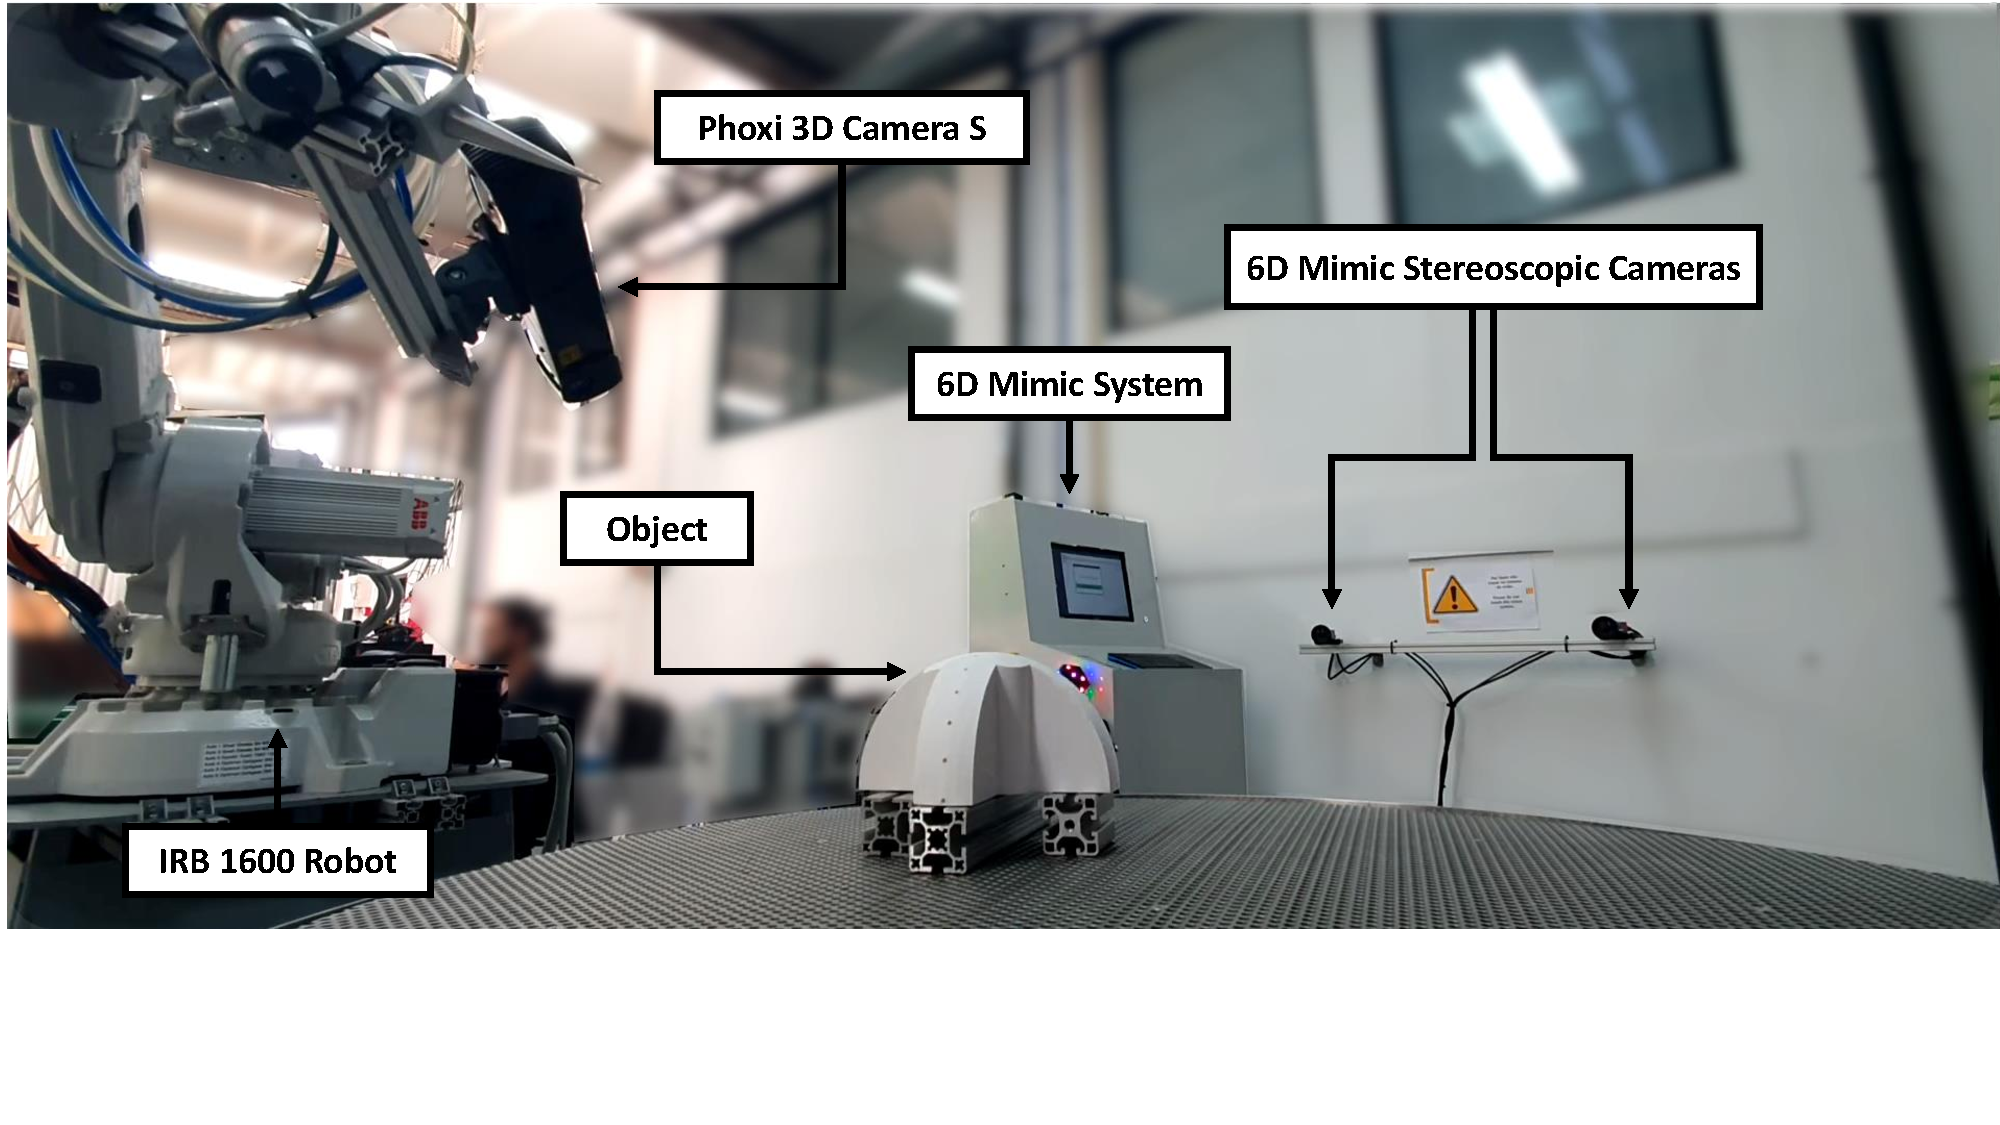
\includegraphics[trim={0cm 3.8cm 0cm 0cm},clip,width=1\linewidth,angle=0]{Cap4/Figuras/photo_use_case_overview_labeled.pdf}}
\end{tcolorbox}
\caption{The proposed use case hardware setup. The Phoxi 3D Camera S is used to locate the object pose. It is attached on a IRB 1600 robot to set a precise acquisition pose. The 6D Mimic system is responsible to detect the handler tool with its stereoscopic cameras.}
\label{fig:use_case_setup}
}%end resize box
\end{figure}




%\subsection{Plugin system management}
%\label{cap4:modular_grasping_architecture:sec:grasping_synthesis:subsec:mimic_grasping:subsubsec:pluginsystem}

%The plugin management is important since different techniques could be implemented as a dynamic library that is loaded in run-time into the mimic grasping architecture without the need to recompile the core pipeline.  



%\subsubsection{Use-case development}
%\label{cap4:modular_grasping_architecture:sec:grasping_synthesis:subsec:mimic_grasping:ware}






%\subsubsection{GUI interface}

\subsubsection{Tool Hardware}
\label{cap4:modular_grasping_architecture:sec:grasping_synthesis:subsec:mimic_grasping:subsubsec:hardware}


A handle tool is designed to a human perform a grasping demonstration, Figure~\ref{fig:tool}. The handler is created following the modular concept since, it need to support different robots' grippers and detection hardware, if needed. Therefore, the human can teach how to grasp with the same gripper used by the robot.% This tool is detect by a tool localisation algorithm which need to be implemented as a plugin into mimic grasping structure. The same is valid to object localisation algorithm.

In addition, the handler supports an Arduino Nano which is embedded into an electronic case (Figure~\ref{fig:tool}), two buttons to open/close the gripper and record/delete grasping, and an RGB LED to visual firmware states feedback. Eletronic schematics is presented in Appendix~\ref{ap:handler_electronic}. The gripper support is a modular part, allowing to quickly change tools Figure~\ref{fig:tool}. The cover is also modular since tool localisation techniques could have different identification devices. The developed tool firmware is discussed in Section \ref{cap4:modular_grasping_architecture:sec:grasping_synthesis:subsec:mimic_grasping:subsubsec:firmware}

\begin{figure}[h!]
\resizebox{.7\textwidth}{!}{%
\begin{tcolorbox}
\centerline{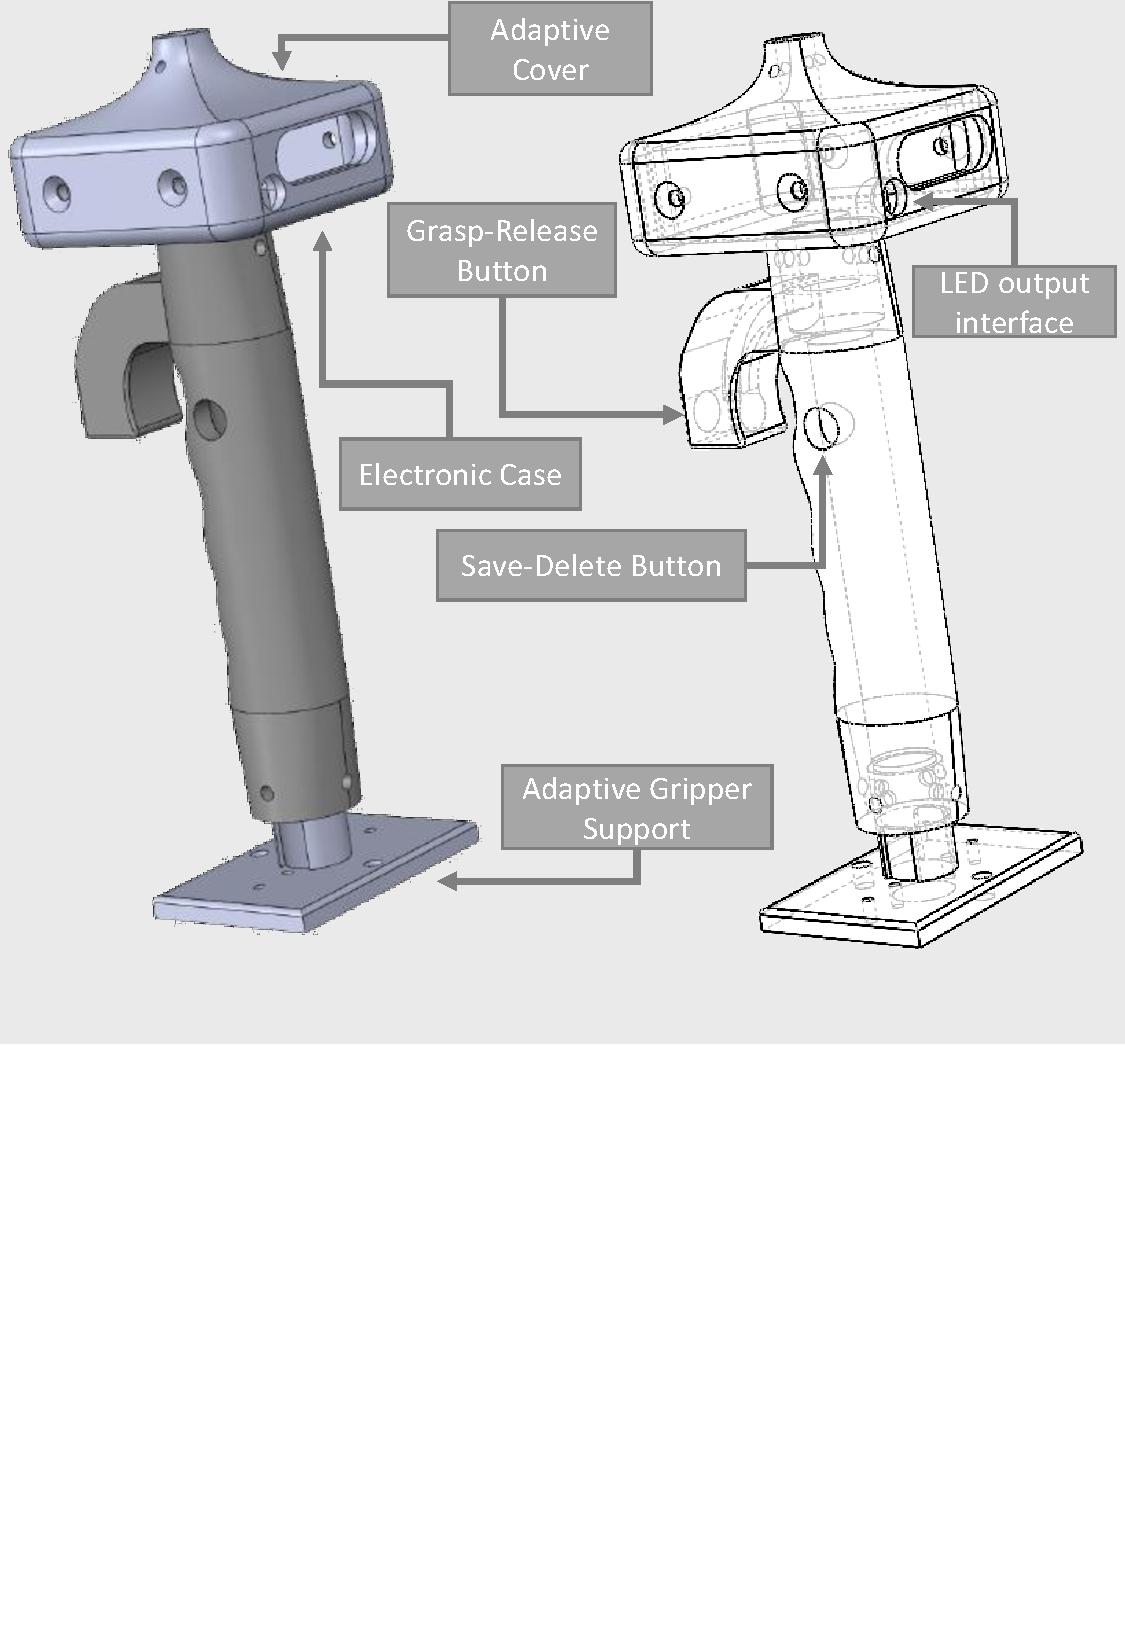
\includegraphics[trim={0cm 11.5cm 0cm 0cm},clip,width=1\linewidth,angle=0]{Cap4/Figuras/mimic_tool_handler.pdf}}
\end{tcolorbox}
\caption{Proposed handler tool.}
\label{fig:tool}}
\end{figure}

For the present thesis, the grippers supported by mimic grasping are: the parallel two-finger gripper HGPC16A~\cite{festo_2f} and the foam suction cup FM-SW 76x22 4x6 N10~\cite{schmalz_cup} (Figure~\ref{fig:mimic_grippers_supported}). It is important to note that the firmware can be easily improved with more types of grippers. Since the supported gripper are pneumatics, a valve system is also designed \cred{TODO}.

\begin{figure}[h!]
\resizebox{.4\textwidth}{!}{%
\begin{tcolorbox}
% \centerline{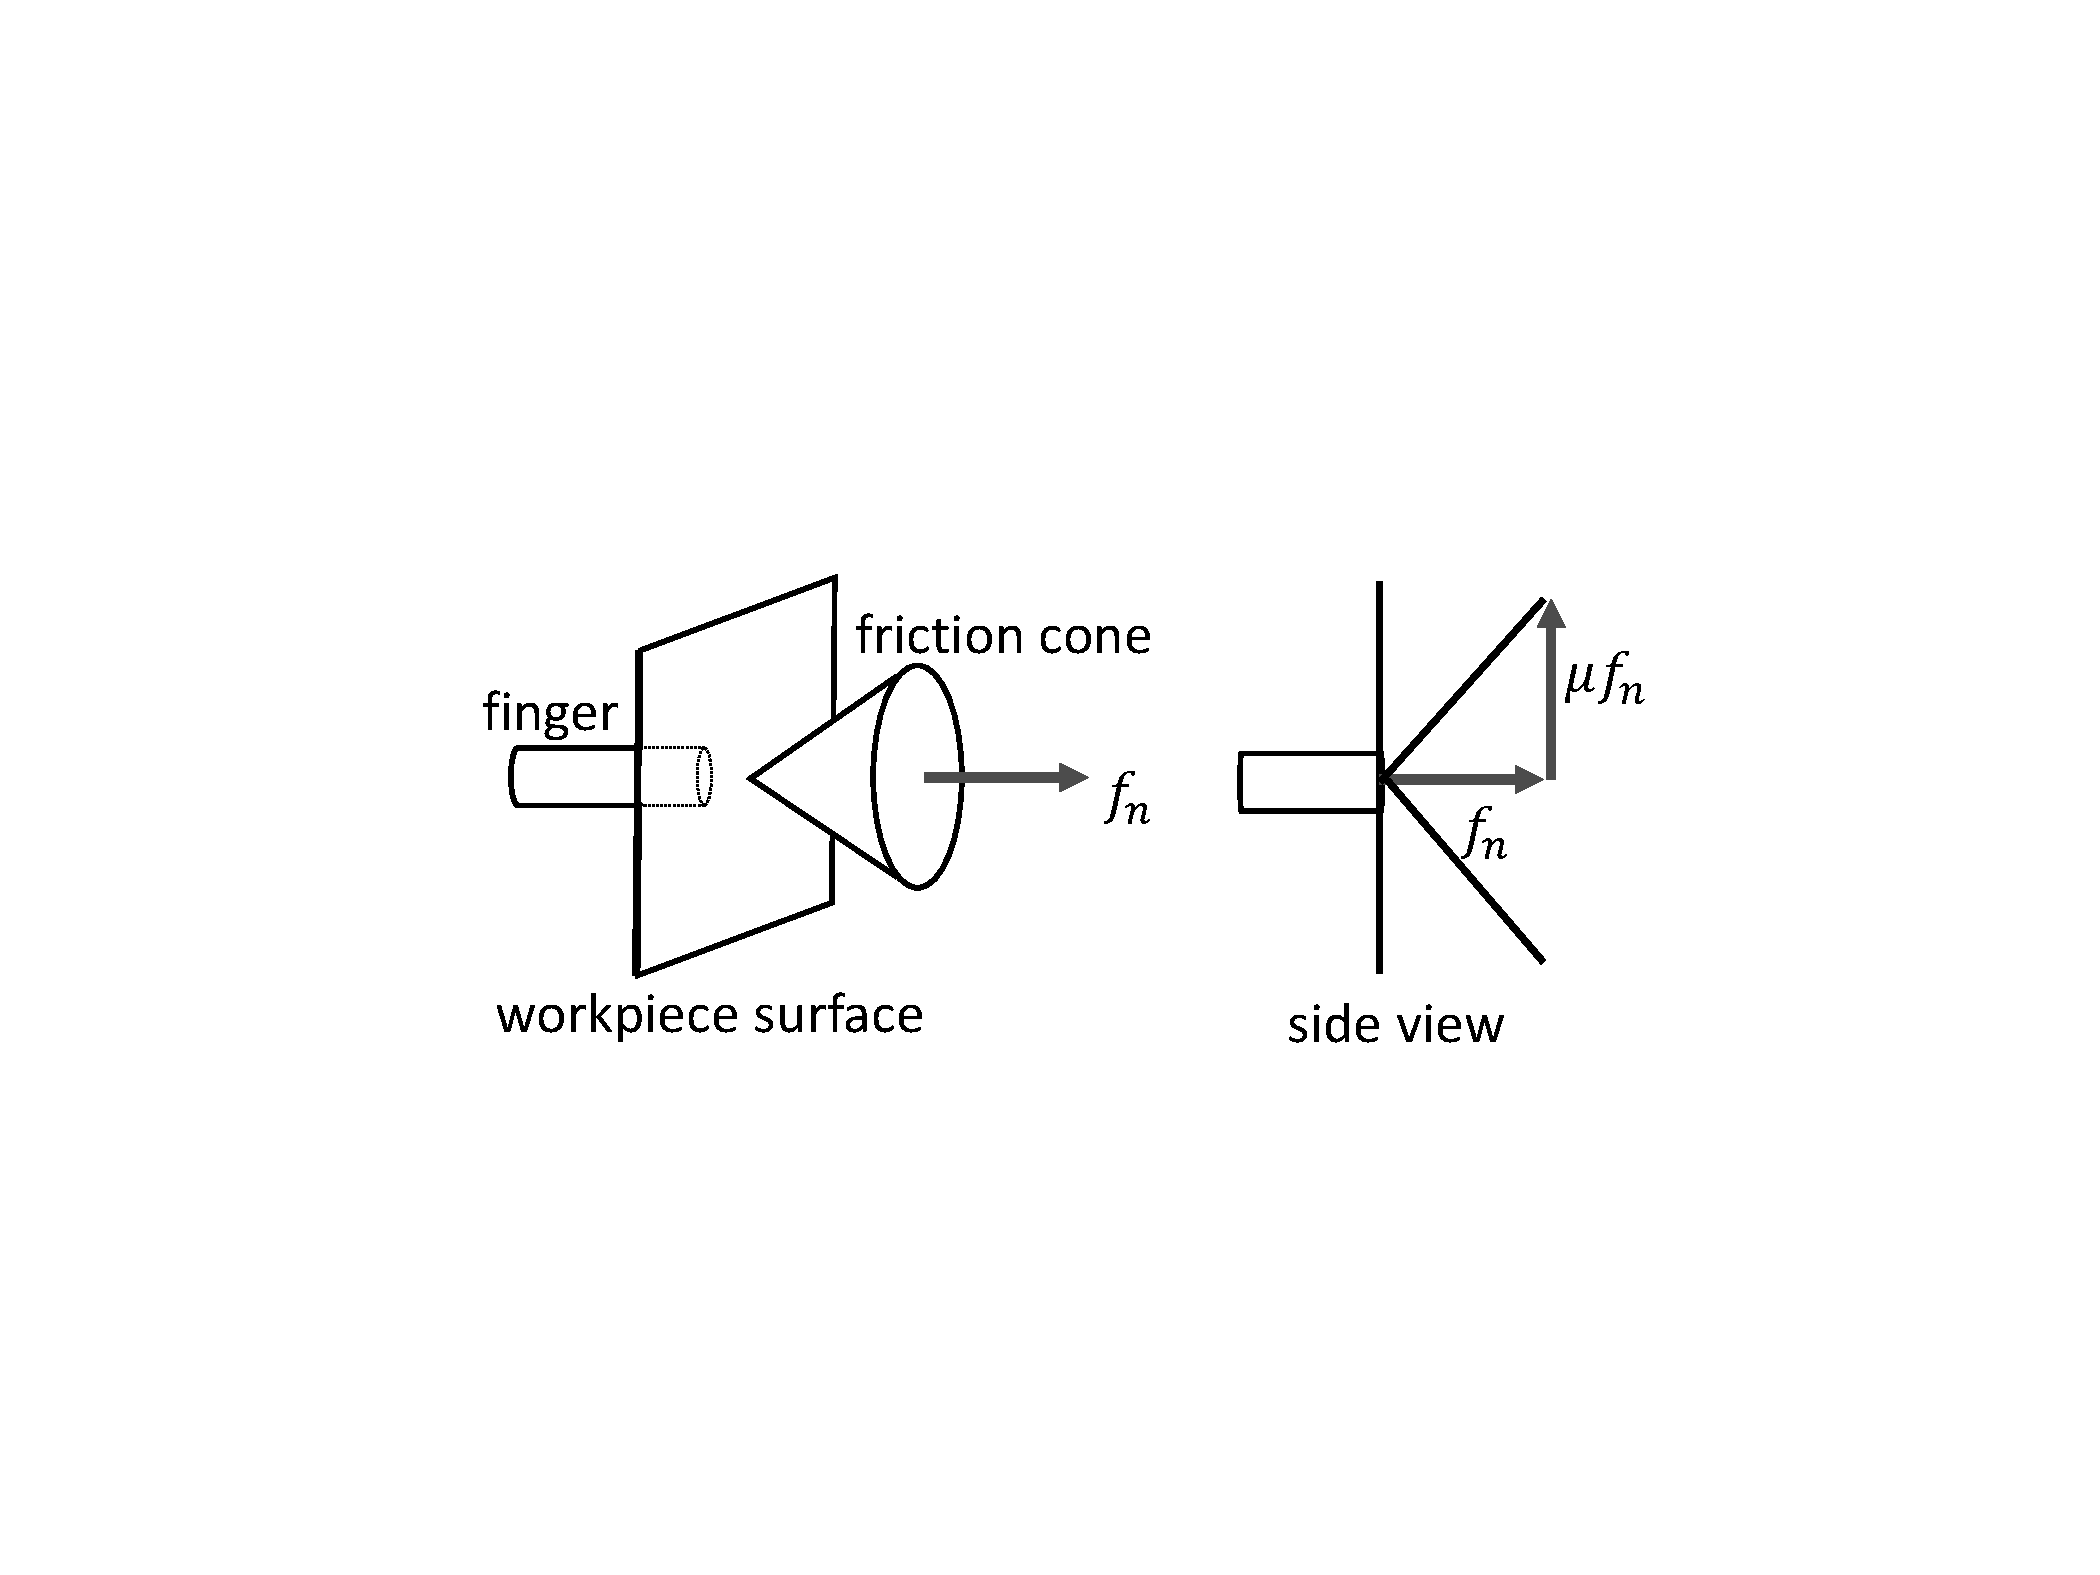
\includegraphics[trim={7cm 8cm 7cm 9cm},clip,width=1\linewidth,angle=0]{Cap2/Figuras/friction_contact.pdf}}
\centerline{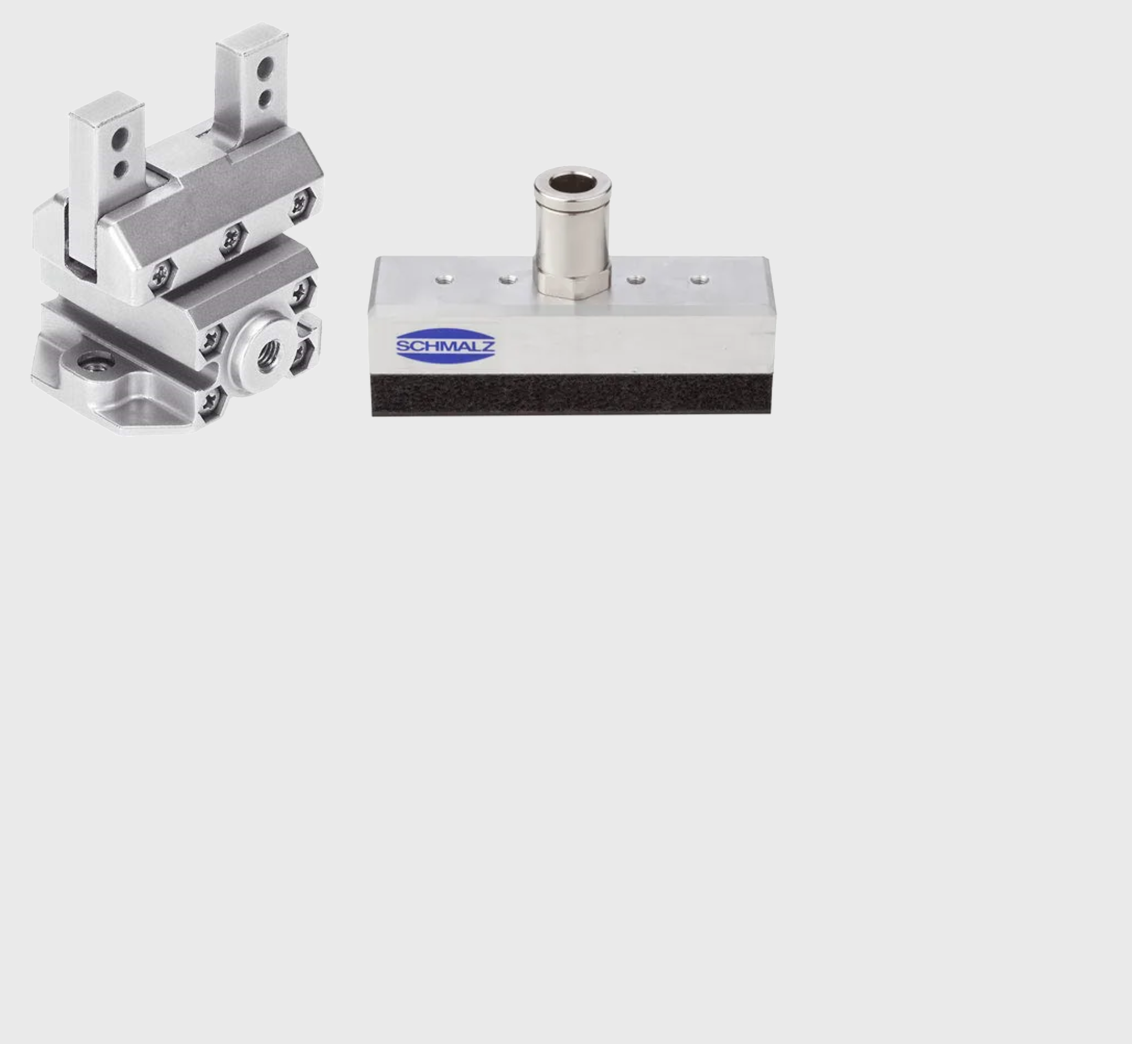
\includegraphics[trim={0cm 10cm 6cm 0cm},clip,width=1\linewidth,angle=0]{Cap4/Figuras/grippers_mimic.pdf}}
\end{tcolorbox}
\caption{HGPC16A and FM-SW 76x22 4x6 N10 grippers.}
\label{fig:mimic_grippers_supported}}
\end{figure}

\subsubsection{Tool Firmware}
\label{cap4:modular_grasping_architecture:sec:grasping_synthesis:subsec:mimic_grasping:subsubsec:firmware}

The firmware is designed to interact with a companion computer with the mimic grasping server working on it. The communication is done by serial with a default baud rate of 115200. The Figure~\ref{fig:mimic_firmware} presents the firmware finite state machine and each state is described bellow:

\begin{figure}[h!]
\resizebox{0.9\textwidth}{!}{%
\begin{tcolorbox}
% \centerline{\includegraphics[trim={7cm 8cm 7cm 9cm},clip,width=1\linewidth,angle=0]{Cap2/Figuras/friction_contact.pdf}}
\centerline{\includegraphics[trim={0cm 17cm 0.8cm 1cm},clip,width=1\linewidth,angle=0]{Cap4/Figuras/mimic_grasping_firmware_state_machine.pdf}}
\end{tcolorbox}
\caption{Proposed firmware finite state machine.}
\label{fig:mimic_firmware}}
\end{figure}

\begin{itemize_jp}
    \item \textbf{Waiting Server:} Idle initial state. It waits for a start command from the server. In the start command message, the gripper type needs to be defined. Output LED state: blink yellow;

    \item \textbf{Running:} Tool running rest state where the user can manipulate it. Only the grasping button is enabled allowing the ``Grasping" transition. Output LED state: solid white;
    
    \item \textbf{Active Gripper:} State that active the grasping. Both buttons are enabled. If the grasping button is pressed the ``Release" transition is activated. Meanwhile, the save button actives the ``Save Request" transition. This state is related to the implemented actuator. Actually, this state only supports pneumatic grippers which are performed by relays usages.  Output LED state: solid cyan;
    
    \item \textbf{Saving: } State which firmware requests the server to acquire data and save it. None of the buttons is enabled. If the server performs the operation successfully the ``Set Success" transition will happen. Otherwise, the ``Error Received" transition is activated. Output LED state: Blink Blue;
    
    \item \textbf{Error:} Only the grasping button is enabled allowing the user to release the work object and leaving the error mode (``Release" transition) to restart the operation. Output LED state: blink red;
    
    \item \textbf{Success:} State that indicates that the grasping pose is correct recorded by the server. Both buttons are enabled. Grasping button pressed actives the ``Release" transition. Holding save button actives the ``Set Cancel`" transition. Output LED state: solid green;
    
    \item \textbf{Cancelling:} State which the firmware requests the server to delete the last acquired grasping. The ``Canceled" transition will only be activated by feedback from the server. 
    
\end{itemize_jp}

All states can be reset by a reset message from the server. Thus, the initial state (waiting server) will take place. A hardware reset is also enabled by holding the grasping button for more than three seconds. The implemented state machine is a Moore Machine with its outputs described by Table~\ref{tab:firmware_state_outputs}.

% Please add the following required packages to your document preamble:
% \usepackage{booktabs}
% \usepackage{multirow}
% \usepackage{graphicx}
\begin{table}[h!]
\resizebox{0.7\textwidth}{!}{%
\begin{tcolorbox}
\centering
\caption{Firmware state's output}
\label{tab:firmware_state_outputs}
\resizebox{1\textwidth}{!}{%
\begin{tabular}{@{}cccc@{}}
\toprule
\multirow{2}{*}{\textbf{State}} & \multicolumn{3}{c}{\textbf{Output}}                                   \\ \cmidrule(l){2-4} 
                       & Active Gripper & Server Save Request & Server Remove Request \\ \midrule
Waiting server         & 0              & 0                   & 0                     \\
Running                & 0              & 0                   & 0                     \\
Active Gripper         & 1              & 0                   & 0                     \\
Success                & 1              & 0                   & 0                     \\
Cancelling             & 1              & 0                   & 1                     \\
Saving                 & 1              & 1                   & 0                     \\
Error                  & 1              & 0                   & 0                     \\ \bottomrule
\end{tabular}%
}
\end{tcolorbox}
}
\end{table}


\subsubsection{6D Mimic Interface}
\label{cap4:modular_grasping_architecture:sec:grasping_synthesis:subsec:mimic_grasping:subsubsec:6dmimic_interface}

The 6D Mimic was first introduced by~\cite{ferreira2016stereo} and improved in current thesis~\cite{6dmimicIMU}, with the objective to facilitate the robot programming in industrial painting procedure. The core relies in tracking a luminous marker movement attached on a painting tool. Stereo cameras are used to perform the marker identification at 25Hz. Therefore, the user can teaching by demonstration the painting procedure to a robot without the need to programming it. In summary, the systems is constituted of a main computer and electronic interface to control the luminous marker.

In the present thesis the 6D Mimic system is used in current Mimic Grasping use-case. The handler tool has attached the luminous marker (see Figure~\ref{fig:handler_with_luminous_marker}),  in the cover support~\ref{fig:tool}, which is properly calibrated with the new tool (the relationship between the marker and the TCP).

\begin{figure}[h!]
\resizebox{0.75\textwidth}{!}{%
\begin{tcolorbox}
\centerline{\includegraphics[trim={0cm 0cm 1cm 0cm},clip,width=0.25\linewidth,angle=-90]{Cap4/Figuras/mimic_grasping_on_handler_2.pdf}}
\end{tcolorbox}
\caption{The mimic handler with 6D Mimic luminous marker attached.}
\label{fig:handler_with_luminous_marker}
}
\end{figure}

A Pascal server is designed into 6D Mimic computer to communicate with Mimic Grasping companion computer~\ref{fig:run_time_test_case_behaviour}. This server is based on 6D Mimic main pipeline, however, it is adapted to generate a grasping candidate. More specifically, when the user request to save a grasping pose (Section~\ref{cap4:modular_grasping_architecture:sec:grasping_synthesis:subsec:mimic_grasping:subsubsec:firmware}) an interface plugin, into Mimic Grasping Module, requests through a \ac{TCP} socket the tool tracking.  The tool pose is defined by the mean value of a pre-defined acquisition time, which default value is three seconds, i.e a mean of 75 measurements. Afterwards, the 6D Mimic computer sends the structured grasping pose through \ac{TCP} back to the plugin interface which passes it to the Mimic Grasping core structure. The implemented 6D mimic server also sends a hearthbit signal ensuring that the computers communication are properly working, otherwise, an error is detected by the plugin interrupting the teaching process.



\subsubsection{\acl{DRL} Interface}
\label{cap4:modular_grasping_architecture:sec:grasping_synthesis:subsec:mimic_grasping:subsubsec:drl_interface}

The \ac{DRL}, proposed by~\cite{COSTA2016113}, was initially developed as a modular robot localisation system but its application is high, being able to be used in object recognition. The configuration to perform this task builds the basis of the \ac{OR}~\cite{or}. This package is structured in \ac{ROS} action service allowing the user to track objects' poses using a CAD reference model and a acquired point cloud image. Detailed description of the technique can be checked at~\cite{COSTA2016113} and~\cite{or}.

The purpose of the present thesis is to deploy this package as a mimic grasping server and plugin to recognize the object pose. Herewith, the grasping candidate generated by the 6D Mimic interface, Section~\ref{cap4:modular_grasping_architecture:sec:grasping_synthesis:subsec:mimic_grasping:subsubsec:6dmimic_interface}, is completely defined. To perform so, Photoneo Phoxi 3D Camera S~\cite{photoneo} is used to point cloud acquisition.


A \ac{ROS} wrapper package to \ac{OR} is created aiming to deploy the server to process the 3D image which comes from a Photoneo Phoxi 3D Camera S~\cite{photoneo}. Both, the server and the camera package are implemented as \ac{ROS} action server, therefore to require the 3D image a goal request is emitted followed by a goal request to process the tracking. These goals are executed by the proposed Phoxi+\ac{DRL} plugin which also load all necessary configurations to package and load the \ac{ROS} environment. It is important to note that eh Mimic Grasping does not have any dependencies with ROS, being the \ac{ROS} prerequisites in charge of the plugin. The related procedure elucidation is exposed in Figure~\ref{fig:run_time_test_case_behaviour}.


\begin{figure}[h!]
\resizebox{1\textwidth}{!}{%
\begin{tcolorbox}
\centerline{\includegraphics[trim={0cm 14cm 10.5cm 0cm},clip,width=1\linewidth,angle=0]{Cap4/Figuras/flowchart_testcase.pdf}}
\end{tcolorbox}
\caption{The plugins are responsible to establish the communication between the localisation strategies and the Mimic Grasping pipeline. 6D Mimic and Phoxi DRL are the implemented interfaces to the proposed use case.}
\label{fig:run_time_test_case_behaviour}
}%end resize box
\end{figure}

\subsubsection{Mimic Grasping \acl{GUI}}
\label{cap4:modular_grasping_architecture:sec:grasping_synthesis:subsec:mimic_grasping:subsubsec:gui}

A \ac{GUI} is designed to allow easy interaction with Mimic Grasping API. The main window is presented in Figure~\ref{fig:main_screen_gui} where the object 3D model is plotted and reference frames indicate the recorded grasping candidate while performing the demonstration. On the right, an output log panel is responsible to inform the mimic grasping core procedure followed by a handler firmware state indicator. Buttons allow the user to start and stop the pipeline and also export the dataset which is also plotted in 3D visualisation. 


\begin{figure}[h!]
\resizebox{0.8\textwidth}{!}{%
\begin{tcolorbox}
\centerline{\includegraphics[trim={0cm 0cm 0cm 0cm},clip,width=1\linewidth,angle=0]{Cap4/Figuras/gui/main_screen_small.pdf}}
\end{tcolorbox}
\caption{\ac{GUI} main window.}
\label{fig:main_screen_gui}
}%end resize box
\end{figure}

The menu interface gives access to configurations such as localisation and firmware setup. The locator configuration is defined in Figure~\ref{fig:localisation_screen_gui}. In this window, the user can define which plugin will be loaded followed by the plugin-specific configuration file, the executor, and terminator commands (Section~\ref{cap4:modular_grasping_architecture:sec:grasping_synthesis:subsec:mimic_grasping}). These configuration can be saved to be used later by the Mimic Grasping API.

\begin{figure}[h!]
\resizebox{0.8\textwidth}{!}{%
\begin{tcolorbox}
\centerline{\includegraphics[trim={0cm 0cm 0cm 0cm},clip,width=1\linewidth,angle=0]{Cap4/Figuras/gui/localisators_config_screen_small.pdf}}
\end{tcolorbox}
\caption{\ac{GUI} localisation configuration window.}
\label{fig:localisation_screen_gui}
}%end resize box
\end{figure}

Regarding the proposed handler firmware, it is possible to communicate, configure it and test it using the firmware window~\ref{fig:firmware_screen_gui}. It is an important configuration menu since needs to be configured according to the gripper attached to the handler.

\begin{figure}[h!]
\resizebox{0.8\textwidth}{!}{%
\begin{tcolorbox}
\centerline{\includegraphics[trim={0cm 0cm 0cm 0cm},clip,width=1\linewidth,angle=0]{Cap4/Figuras/gui/tool_firmware_screen_small.pdf}}
\end{tcolorbox}
\caption{\ac{GUI} firmware configuration window.}
\label{fig:firmware_screen_gui}
}%end resize box
\end{figure}


\subsection{Post-Processor Pipeline}
\label{cap4:modular_grasping_architecture:sec:grasping_synthesis:subsec:post_processor}

The post-processor pipeline is a software structure based on \ac{ROS} framework responsible to edit and manipulate the datatasets in a pipeline workflow structure defined by a YAML configuration file. The Figure~\ref{fig:grasping_post_processor} presents the Post-processor pipeline workflow.

\begin{figure}[h!]
\resizebox{1\textwidth}{!}{%
\begin{tcolorbox}
\centerline{\includegraphics[trim={0.25cm 6cm 14.75cm 0cm},clip,width=1\linewidth,angle=0]{Cap4/Figuras/flowchart_post_processors_pipeline.drawio.pdf}}
\end{tcolorbox}
\caption{Post-processor pipeline workflow.}
\label{fig:grasping_post_processor}
}%end resize box
\end{figure}

A YAML pipeline configuration file is responsible to define the cascade of methods to be deployed, Snippet~\ref{code:post_processor_config}. It is mandatory that the first method be a unique loader method. The loader is responsible to import the dataset to be used by the following ``post-processor`" methods.

\begin{snippet}[h!]
\centering
\resizebox{0.75\textwidth}{!}{%
	\begin{tcolorbox}
 \lstinputlisting[
                  %caption= Post-processor pipeline configuration example.,
                  abovecaptionskip=3pt,
                  captionpos=b,
                  style=yaml,
                  linerange={0-18},
                  firstnumber=25,
                  %label=code:post_processor_config
                  ]
                  {Cap4/codes/post_processor_config.yaml}
\end{tcolorbox}
}
\caption{Post-processor pipeline configuration example.}
\label{code:post_processor_config}
\end{snippet}



Since the ``Post-processor'' pipeline architecture code design is based on polymorphism, which is implemented in C++, the server allows being incremented with new heuristics classes that inherit a defined parent class. Therefore new approaches can be easily integrated without modifying the core architecture and pipeline workflow. 

The proposed post-processors methods are described in the Sections~\ref{cap4:modular_grasping_architecture:sec:grasping_synthesis:subsec:graspit:subsubsec:loader} to ~\ref{cap4:modular_grasping_architecture:sec:grasping_synthesis:subsec:graspit:subsubsec:graspit_viewer}.

\subsubsection{Loader}
\label{cap4:modular_grasping_architecture:sec:grasping_synthesis:subsec:graspit:subsubsec:loader}

The Loader allows to import a already created dataset into ``Post-processor'' pipeline. It important to note that the dataset should follow the proposed convention described in Section~\ref{cap4:modular_grasping_architecture:sec:grasping_dataset}. It also allows to merge several different datasets into one. The loader YAML descriptor is defined in Snippet~\ref{code:load_datatset_feeder}. %and its parameters is presented below:

%\begin{minipage}{1\textwidth} 
\begin{snippet}[h!]
\centering
\resizebox{0.75\textwidth}{!}{%
\begin{tcolorbox}
 \lstinputlisting[%caption= Load dataset YAML descriptor example.,
                  abovecaptionskip=3pt,
                  captionpos=b,
                  style=yaml,
                  linerange={0-4},
                  firstnumber=25,
                  %label=code:load_datatset_feeder
                  ]
                  {Cap4/codes/load_feeder.yaml}
\end{tcolorbox}
}
\caption{Load dataset YAML descriptor example.}
\label{code:load_datatset_feeder}
\end{snippet}
%\end{minipage}

The object name is necessary and described by ``$model$\_$file$\_$name$'' parameter since each dataset is characterized over an specific object. It is possible to load more than one dataset and the number loadings is defined by ``$number$\_$of$\_$files$'' and a namespace is needed by filing the ``$ns$\_$filename$\_$of$\_$candidates$'' parameter. The namespace is necessary to differ candidates from different datatsets. 

%\begin{itemize_jp}
%    \item \textbf{model$\_$file$\_$name:} the object name since each dataset is defined over an specific object;
%    \item \textbf{number$\_$of$\_$files:} number of datatsets to be loaded.;
%    \item \textbf{ns$\_$filename$\_$of$\_$candidates:} namespace to differ candidates from different datatsets.
%\end{itemize_jp}

\subsubsection{Distance Filter Post-Processor}
\label{cap4:modular_grasping_architecture:sec:grasping_synthesis:subsec:postprocessor:subsubsec:distance_filter}

In the grasping dataset some candidates could be in duplicate. Therefore a relevance filter based on distance is proposed to eliminate redundancies. It estimates the tridimensional euclidean and the angular (roll, pitch and yaw) distances between all candidates in dataset. If these distances are absolute smaller than the specific configuration threshold, in meters for euclidean and in degrees for the angular, a duplicate is detected and the candidate replica is deleted from dataset. The pipeline descriptor for this post-processor is presented in Snippet~\ref{code:distance_filter}.% and its parameters are described below:

\begin{snippet}[h!]
\centering
\resizebox{0.75\textwidth}{!}{%
\begin{tcolorbox}
 \lstinputlisting[caption= Distance filter post-processor YAML descriptor example.,
                  abovecaptionskip=3pt,
                  captionpos=b,
                  style=yaml,
                  linerange={0-5},
                  firstnumber=25,
                  label=code:distance_filter]
                  {Cap4/codes/distance_filter.yaml}
\end{tcolorbox}
}
\end{snippet}

%\begin{itemize_jp}
%    \item \textbf{abs$\_$euclidean$\_$distance$\_$threshold}: absolute euclidean minimum distance (in meters) acceptable to define a non-duplicate candidate;  
%    \item \textbf{abs$\_$roll$\_$distance$\_$threshold}: absolute roll minimum distance (in degrees) acceptable to define a non-duplicate candidate; 
%    \item \textbf{abs$\_$pitch$\_$distance$\_$threshold}: absolute pitch minimum distance (in degrees) acceptable to define a non-duplicate candidate; 
%    \item \textbf{abs$\_$yaw$\_$distance$\_$threshold}: absolute yaw minimum distance (in degrees) acceptable to define a non-duplicate candidate;
%\end{itemize_jp}

\subsubsection{Tool Center Point Angle Twin}
\label{cap4:modular_grasping_architecture:sec:grasping_synthesis:subsec:postprocessor:subsubsec:tcp_angle_twin}

According to the gripper type, some candidates replica could be acceptable. Considering the symmetry over the TCP normal axis, it is possible to define an angular twin replica without the search algorithm, thus reducing processing. E.g. two-finger grippers could have a mirror twin (180 degrees over attack axis, Figure~\ref{fig:tcp_angle_twin}) with same grasping properties. Therefore, the TCP angle twin post-processor is designed to apply this replica operation overall dataset. It builds a candidate twin based on an angular shift (Tait-Briant ZYX-order) over the TCP reference frame.  The pipeline descriptor in Snippet~\ref{code:tcp_angle_twin} is an example of generating candidates twin with a 180 degrees angle displacement over the TCP Z-axis. Others axis can also compose the displacement, individually or in association, by setting the $Rx$, $Ry$ and $Rz$ parameters.

\begin{figure}[h!]
\resizebox{1\textwidth}{!}{%
\begin{tcolorbox}
\centerline{\includegraphics[trim={3cm 3cm 3cm 3cm},clip,width=1\linewidth,angle=0]{Cap4/Figuras/tcp_angle_twin.pdf}}
\end{tcolorbox}
\caption{Symmetric grasping replicas over a TCP's symmetry axis.}
\label{fig:tcp_angle_twin}
}%end resize box
\end{figure}

%\begin{minipage}{1\textwidth} 
\begin{snippet}[h!]
\centering
\resizebox{0.75\textwidth}{!}{%
\begin{tcolorbox}
 \lstinputlisting[%caption= TCP angle twin post-processor YAML descriptor example.,
                  abovecaptionskip=3pt,
                  captionpos=b,
                  style=yaml,
                  linerange={0-5},
                  firstnumber=25,
                  %label=code:tcp_angle_twin
                  ]
                  {Cap4/codes/tcp_angle_twin.yaml}
\end{tcolorbox}
}
\caption{TCP angle twin post-processor YAML descriptor example}
\label{code:tcp_angle_twin}
\end{snippet}
%\end{minipage}

%\begin{itemize_jp}
%    \item \textbf{Rz:} angle displacement (in degrees) over the TCP Z-axis.
%    \item \textbf{Ry:} angle displacement (in degrees) over the TCP Y-axis.
%    \item \textbf{Rx:} angle displacement (in degrees) over the TCP X-axis.
%\end{itemize_jp}

This post-processor generates only one symmetric replica per grasping candidate. If more is needed, this filter can be applied several times in sequence, following by Distance Filter~\ref{cap4:modular_grasping_architecture:sec:grasping_synthesis:subsec:postprocessor:subsubsec:distance_filter} to remove duplicates.

\subsubsection{Object Angle Twin}
\label{cap4:modular_grasping_architecture:sec:grasping_synthesis:subsec:postprocessor:subsubsec:obj_angle_twin}

Some objects are spherical or radial symmetries, thus some grasping candidates could have symmetric representation~\ref{fig:obj_angle_twin}. Therefore, this could be automatically generated by the object angle twin replica post-processor. This characteristic could improve the candidates' search. It build a candidate twin based on a spherical angular shift (azimuth and/or polar angle) over the object reference frame. The radius corresponds to the candidate position, therefore it is not a parameter. It is important to note that, the object reference frame should be defined as spherical/radial symmetry origin, otherwise this post-processor will not correctly work. The Snippet~\ref{code:obj_angle_twin} shows an configuration example to build grasping candidates replicas with $30^o$ of azimuth displacement.

\begin{figure}[h!]
\resizebox{1\textwidth}{!}{%
\begin{tcolorbox}
\centerline{\includegraphics[trim={1cm 0.75cm 10cm 0.5cm},clip,width=1\linewidth,angle=0]{Cap4/Figuras/obj_angle_twin.pdf}}
\end{tcolorbox}
\caption{Symmetric grasping replicas over a object's symmetry axis.}
\label{fig:obj_angle_twin}
}%end resize box
\end{figure}

%\begin{minipage}{1\textwidth} 
\begin{snippet}[h!]
\centering
\resizebox{0.75\textwidth}{!}{%
\begin{tcolorbox}
 \lstinputlisting[%caption= OBJ angle twin post-processor YAML descriptor example.,
                  abovecaptionskip=3pt,
                  captionpos=b,
                  style=yaml,
                  linerange={0-5},
                  firstnumber=25,
                  %label=code:obj_angle_twin
                  ]
                  {Cap4/codes/obj_angle_twin.yaml}
\end{tcolorbox}
}
\caption{Object angle twin post-processor YAML descriptor example}
\label{code:obj_angle_twin}
\end{snippet}
%\end{minipage}

%\begin{itemize_jp}
%    \item \textbf{azimuth:} azimuth angle displacement (in degrees) over the object reference frame;
%    \item \textbf{polar:} azimuth angle displacement in degrees) over the object reference frame;
%\end{itemize_jp}

To correctly deploy the spherical displacement over a candidate, the following relationship between spherical coordinates and transformation matrix is deployed:

\begin{equation}
T=\begin{bmatrix}
cos(\Theta) & sin(\Theta)\cdot cos(\phi) & sin(\Theta)\cdot sin(\phi) \\
-sin(\Theta)& cos(\Theta)\cdot cos(\phi)& cos(\Theta)\cdot sin(\phi) \\
0 & -sin(\phi) & cos(\phi)
\end{bmatrix}
\end{equation}



\subsubsection{Viewer based post-processors}
\label{cap4:modular_grasping_architecture:sec:grasping_synthesis:subsec:postprocessor:subsubsec:viewers}

Two post-processors are implemented to grasping candidates visualisation: the ``GraspIt!''~\cite{miller2004graspit} and the RViz~\cite{rviz} viewer. The viewer post-processor configures, builds the visualisation world and calls the respective 3D environment. It also loads the dataset and set the candidate's configuration to visualisation. A menu is responsible for waiting for the user input to run over the dataset. This tool is important for visual inspection of the dataset.

To ``GraspIt!'' support visualisation, the XML 3D model and the Polygon File Format (extension ``.ply'') need to be defined to gripper and object, respectively. In other hand, to RViz, a URDF 3D model is expected following by the object's Polygon File Format. The viewer module implementation should takes in consideration which gripper is used to correctly map the DOFs of each URDF joint. Therefore, the candidates' parameters ``$method/type$" and ``$gripper/type$"  (Section~\ref{cap4:modular_grasping_architecture:sec:grasping_dataset}) lead to help this mapping, since both defined how to read the array parameter \ac{DOF}. Each viewer YAML descriptor are presented in Snippet~\ref{code:graspit_viewer} and~\ref{code:rviz_viewer} : 

%\begin{minipage}{1\textwidth} 
\begin{snippet}[h!]
\centering
\resizebox{0.75\textwidth}{!}{%
\begin{tcolorbox}
 \lstinputlisting[%caption= ``GraspIt!" viewer YAML descriptor example.,
                  abovecaptionskip=3pt,
                  captionpos=b,
                  style=yaml,
                  linerange={0-5},
                  firstnumber=25,
                  %label=code:graspit_viewer
                  ]
                  {Cap4/codes/graspit_viewer.yaml}
\end{tcolorbox}
}
\caption{``GraspIt!" viewer YAML descriptor example.}
\label{code:graspit_viewer}
\end{snippet}
%\end{minipage}

%\begin{minipage}{1\textwidth} 
\begin{snippet}[h!]
\centering
\resizebox{0.75\textwidth}{!}{%
	\begin{tcolorbox}
 \lstinputlisting[%caption= Rviz viewer YAML descriptor example.,
                  abovecaptionskip=3pt,
                  captionpos=b,
                  style=yaml,
                  linerange={0-5},
                  firstnumber=25,
                  %label=code:rviz_viewer
                  ]
                  {Cap4/codes/rviz_viewer.yaml}
\end{tcolorbox}
}
\caption{Rviz viewer YAML descriptor example.}
\label{code:rviz_viewer}
\end{snippet}
%\end{minipage}

%TODO: insert images

%\subsubsection{ROS Viewer}
%\label{cap4:modular_grasping_architecture:sec:grasping_synthesis:subsec:graspit:subsubsec:ros%_viewer}

\section{Grasping Selection}
\label{cap4:modular_grasping_architecture:sec:grasp_selection}

The grasping selection is a \ac{ROS} package (based on \ac{ROS} action server library \cite{ros_action_lib}) designed for choosing the best candidate over a set of previously taught grasping poses of an object. This step is an online procedure; i.e., it is a run-time process performed during the robot task execution. Thus, this operation needs to be fast and reliable. An illustration of the described procedure is presented in Figure~\ref{fig:grasp_estimation}. 

\begin{figure}[h!]
\resizebox{1\textwidth}{!}{%
\begin{tcolorbox}
\centerline{\includegraphics[trim={0cm 0cm 0cm 0cm},clip,width=1\linewidth,angle=0]{Cap4/Figuras/grasping_gray_bg.pdf}}
\end{tcolorbox}
\caption{The grasping selection process. (top~left) The object with the grasping candidates frames. (top~right) The best candidate is chose following the task oriented grasping heuristic. (bottom~left) Robot's initial pose. (bottom~middle) Approaching movement. (bottom~right) Grasping. }
\label{fig:grasp_estimation}
}%end resize box
\end{figure}


Once the candidates dataset are loaded in the parameter server (Figure~\ref{fig:grasping_selection_flowchart}), the grasping selection pipeline estimates the best candidate for allowing the robot to pick the object. The best grasping candidate is chosen according to a cascade of heuristics defined by the user in a YAML file for each object detected (Snippet~\ref{code:selection_pipeline_ex}). Therefore, the object needs to be identified and localised before the grasping selection process. The heuristics cascade gives a score for each grasping candidate related to a reference frame (such as the gripper). The one with the lower cost is the eligible candidate. It is possible to define a weight for each heuristic in the pipeline based on the importance level of each method in the application.

%\begin{minipage}[h!]{1\textwidth}
\begin{snippet}[h!]
\centering
\resizebox{0.75\textwidth}{!}{%
	\begin{tcolorbox}
 \lstinputlisting[%caption= A grasping selection pipeline configuration example.,
                  abovecaptionskip=3pt,
                  captionpos=b,
                  style=yaml,
                  linerange={0-13},
                  firstnumber=25,
                  %label=code:selection_pipeline_ex
                  ]
                  {Cap4/codes/grasping_selection_pipeline.yaml}
\end{tcolorbox}
}
\caption{A grasping selection pipeline configuration example.}
\label{code:selection_pipeline_ex}
\end{snippet}
%\end{minipage}

Since loading the dataset into server demands time, the pipeline allow two types of operation mode: the direct estimation and the pre-load support. The first loads the dataset into rosparam server every time a ROS action's goal request is sent. In other hand, in pre-load support the pipeline requests two ROS action's goals. The first one to load the database into server and the second one to run the estimation pipeline. It is useful to accelerate the procedure. However the user need to be sure that the loaded database correspond to the object in use when run the estimation process (Figure~\ref{fig:grasping_selection_flowchart}).

\begin{figure}[h!]
\resizebox{0.75\textwidth}{!}{%
\begin{tcolorbox}
\centerline{\includegraphics[trim={2.5cm 3cm .5cm 0cm},clip,width=1\linewidth,angle=0]{Cap4/Figuras/grasping_selection_pipeline_workflow.pdf}}
\end{tcolorbox}
\caption{Grasping selection pipeline workflow.}
\label{fig:grasping_selection_flowchart}
}%end resize box
\end{figure}

The grasping selection architecture code design is based on polymorphism and implemented in C++. The grasping selection server allows being incremented with new heuristics classes that inherit a defined parent class. Therefore new approaches can be easily integrated without modifying the grasping selection core architecture and pipeline workflow.  

% TODO: \cred{inserir uml?}


The implemented heuristics for the present thesis proposal are presented from Sections~\ref{cap4:modular_grasping_architecture:sec:grasp_selection:subsec:depth_distance} to~\ref{cap4:modular_grasping_architecture:sec:grasp_selection:subsec:collision_filter}

\subsection{Depth Distance Scorer}
\label{cap4:modular_grasping_architecture:sec:grasp_selection:subsec:depth_distance}

The Depth distance scorer is a method to set the grasping candidate cost value according to the depth distance between the TCP  reference frame and the candidate. Therefore, this cost allows selecting candidates close to depth from the current gripper pose. This is useful for grasping objects in a stack where only height removal layers are considered. The pipeline descriptor is presented in Snippet \ref{code:depth_distance_scorer} and two parameters define it: ``$weight$'' which is a penalty weight value that is inversely proportional to the importance of the metric (thus, this value must be higher than 1); $``distance$\_$threshold''$ the maximum value of distance that is allowed to a candidate, otherwise, it will be discarded.

%\begin{itemize_jp}
%    \item \textbf{weight:} a penalty weight value. The importance of the metric in selection pipeline is inversely proportional to the weight value. Therefore, this value must be higher than 1.
%    \item \textbf{distance$\_$threshold:} candidates with a distance bigger than the threshold value are discarded.
%\end{itemize_jp}


%\begin{minipage}{1\textwidth} 
\begin{snippet}[h!]
\centering
\resizebox{0.75\textwidth}{!}{%
	\begin{tcolorbox}
 \lstinputlisting[%caption= Depth distance scorer pipeline descriptor example.,
                  abovecaptionskip=3pt,
                  captionpos=b,
                  style=yaml,
                  linerange={0-10},
                  firstnumber=25,
                  %label=code:depth_distance_scorer
                  ]
                  {Cap4/codes/depth_distance.yaml}
\end{tcolorbox}
}
\caption{Depth distance scorer pipeline descriptor example.}
\label{code:depth_distance_scorer}
\end{snippet}
%\end{minipage}

\subsection{Euclidean Distance Scorer}
\label{cap4:modular_grasping_architecture:sec:grasp_selection:subsec:euclidean_distance}

The euclidean distance scorer sets the grasping candidate cost value according to the Euclidean distance between the TCP  reference frame and the candidate. This cost allows choosing near candidates from the current gripper pose considering all three dimensions, contrary to the Depth Distance Scorer which only considers one dimension. Therefore, this heuristics is useful to less effort metrics. The pipeline descriptor is presented in Snippet \ref{code:euclidean_distance_scorer} and its parameters are similar to the Depth Distance Scorer, i.e., an ``$weight$'' that defines the importance of the metric and the $``distance$\_$threshold''$ which excludes candidates that extrapolate that value.

%its parameters is described below:

%\begin{itemize_jp}
%    \item \textbf{weight:} a penalty weight value. The importance of the metric in selection pipeline is inversely proportional to the weight value. Therefore, this value must be higher than 1.
%    \item \textbf{distance$\_$threshold:} candidates with a distance bigger than the threshold value are discarded.
%\end{itemize_jp}


%\begin{minipage}{1\textwidth} 
\begin{snippet}[h!]
\centering
\resizebox{0.75\textwidth}{!}{%
	\begin{tcolorbox}
 \lstinputlisting[%caption= Euclidean distance scorer pipeline descriptor example.,
                  abovecaptionskip=3pt,
                  captionpos=b,
                  style=yaml,
                  linerange={0-10},
                  firstnumber=25,
                  %label=code:euclidean_distance_scorer
                  ]
                  {Cap4/codes/euclidean_distance.yaml}
\end{tcolorbox}
}
\caption{Euclidean distance scorer pipeline descriptor example}
\label{code:euclidean_distance_scorer}
\end{snippet}
%\end{minipage}

\subsection{\acl{COG} Distance Scorer}
\label{cap4:modular_grasping_architecture:sec:grasp_selection:subsec:cog_distance}

The \ac{COG} distance scorer is a method to set the grasping candidate cost value according with the euclidean distance between the candidate and the object reference frame. This cost is important in cases of high dimensional objects, which grasping poses can cause torques over the centre of gravity and, affect the equilibrium in grasping movements. The pipeline descriptor is presented in Snippet \ref{code:cog_distance_scorer} and its parameters are the ``$weight$'' that defines the importance of the metric and the $``distance$\_$threshold''$ which excludes candidates that extrapolate that value.

%\begin{itemize_jp}
%    \item \textbf{weight:} a penalty weight value. The importance of the metric in selection pipeline is inversely proportional to the weight value. Therefore, this value must be higher than 1.
%    \item \textbf{distance$\_$threshold:} candidates with a distance bigger than the threshold value are discarded.
%\end{itemize_jp}


%\begin{minipage}{1\textwidth} 
\begin{snippet}[h!]
\centering
\resizebox{0.75\textwidth}{!}{%
	\begin{tcolorbox}
 \lstinputlisting[%caption= COG distance scorer pipeline descriptor example.,
                  abovecaptionskip=3pt,
                  captionpos=b,
                  style=yaml,
                  linerange={0-10},
                  firstnumber=25,
                  %label=code:cog_distance_scorer
                  ]
                  {Cap4/codes/cog_distance.yaml}
\end{tcolorbox}
}
\caption{\ac{COG} distance scorer pipeline descriptor example.}
\label{code:cog_distance_scorer}
\end{snippet}
%\end{minipage}

\subsection{\acl{COBB} Distance Scorer}
\label{cap4:modular_grasping_architecture:sec:grasp_selection:subsec:cobb_distance}

Following the same motivation of \ac{COG} distance scorer\ref{cap4:modular_grasping_architecture:sec:grasp_selection:subsec:cog_distance}, the \ac{COBB} distance scorer defines the grasping candidate cost based on the Euclidean distance between the candidate and the object bounding box reference frame. The difference relies on objects that the mass is not important with but only the dimensions. The pipeline descriptor is presented in Snippet \ref{code:cog_distance_scorer} and its parameters are the ``$weight$'' that defines the importance of the metric and the $``distance$\_$threshold''$ which excludes candidates that extrapolate that value.

\begin{itemize_jp}
    \item \textbf{weight:} a penalty weight value. The importance of the metric in selection pipeline is inversely proportional to the weight value. Therefore, this value must be higher than 1.
    \item \textbf{distance$\_$threshold:} candidates with a distance bigger than the threshold value are discarded.
\end{itemize_jp}


%\begin{minipage}{1\textwidth} 
\begin{snippet}[h!]
\centering
\resizebox{0.75\textwidth}{!}{%
	\begin{tcolorbox}
 \lstinputlisting[%caption= COG distance scorer pipeline descriptor example.,
                  abovecaptionskip=3pt,
                  captionpos=b,
                  style=yaml,
                  linerange={0-10},
                  firstnumber=25,
                  %label=code:cobb_distance_scorer
                  ]
                  {Cap4/codes/cobb_distance.yaml}
\end{tcolorbox}
}
\caption{\ac{COBB} distance scorer pipeline descriptor example.}
\label{code:cobb_distance_scorer}
\end{snippet}
%\end{minipage}

\subsection{Roll Distance Scorer}
\label{cap4:modular_grasping_architecture:sec:grasp_selection:subsec:roll_distance}

The roll distance scorer is a less effort angle displacement selector. Since the ``Grasping Selection`'' Pipeline core relies on configurability, the angles and distance heuristics are developed independently once the application could only take into consideration only a single rotation axis.

This method set the grasping candidate cost value according to the roll distance (TCP X-axis rotation) between the TCP reference frame and the candidate. The pipeline descriptor is presented in Snippet \ref{code:roll_distance_scorer} and besides the already discussed $``weight''$ , two other threshold parameters define the configuration: $``min$\_$angle$\_$threshold`''$ and $``max$\_$angle$\_$threshold`''$ whose are the bound limits in degrees to accept candidates, i.e., it is accepted only candidates within these angular distances.


% its parameters is described below:
%
%\begin{itemize_jp}
%    \item \textbf{weight:} a penalty weight value. The importance of the metric in selection pipeline is inversely proportional to the weight value. Therefore, this value must be higher than 1.
%    \item \textbf{min$\_$angle$\_$threshold:} candidates with a distance lesser than the threshold value are discarded.
%    \item \textbf{max$\_$angle$\_$threshold:} candidates with a distance bigger than the threshold value are discarded.
%\end{itemize_jp}


%\begin{minipage}{1\textwidth} 
\begin{snippet}[h!]
\centering
\resizebox{0.75\textwidth}{!}{%
	\begin{tcolorbox}
 \lstinputlisting[%caption= Roll distance scorer pipeline descriptor example.,
                  abovecaptionskip=3pt,
                  captionpos=b,
                  style=yaml,
                  linerange={0-10},
                  firstnumber=25,
                  %label=code:roll_distance_scorer
                  ]
                  {Cap4/codes/roll_distance.yaml}
\end{tcolorbox}
}
\caption{Roll distance scorer pipeline descriptor example}
\label{code:roll_distance_scorer}
\end{snippet}
%\end{minipage}

\subsection{Pitch Distance Scorer}
\label{cap4:modular_grasping_architecture:sec:grasp_selection:subsec:pitch_distance}

Similarly to Roll Distance scorer\ref{cap4:modular_grasping_architecture:sec:grasp_selection:subsec:roll_distance}, the Pitch Distance Scorer sets the grasping candidate cost value according to the pitch distance between the TCP reference frame and the candidate. Therefore, this cost allows the selection of candidates with less effort in TCP Y-axis rotation. The pipeline descriptor is presented in Snippet \ref{code:pitch_distance_scorer} and its parameters are the same from Roll Distance Scorer, $``weight''$, $``min$\_$angle$\_$threshold`''$ and $``max$\_$angle$\_$threshold`''$.



%\begin{itemize_jp}
%    \item \textbf{weight:} a penalty weight value. The importance of the metric in selection pipeline is inversely proportional to the weight value. Therefore, this value must be higher than 1.
%    \item \textbf{min$\_$angle$\_$threshold:} candidates with a distance lesser than the threshold value are discarded.
%    \item \textbf{max$\_$angle$\_$threshold:} candidates with a distance bigger than the threshold value are discarded.
%\end{itemize_jp}


%\begin{minipage}{1\textwidth} 
\begin{snippet}
\centering
\resizebox{0.75\textwidth}{!}{%
\begin{tcolorbox}
 \lstinputlisting[%caption= Pitch distance scorer pipeline descriptor example.,
                  abovecaptionskip=3pt,
                  captionpos=b,
                  style=yaml,
                  linerange={0-10},
                  firstnumber=25,
                  %label=code:pitch_distance_scorer
                  ]
                  {Cap4/codes/pitch_distance.yaml}
\end{tcolorbox}
}
\caption{Pitch distance scorer pipeline descriptor example.}
\label{code:pitch_distance_scorer}
\end{snippet}
%\end{minipage}

\subsection{Yaw Distance Scorer}
\label{cap4:modular_grasping_architecture:sec:grasp_selection:subsec:yaw_distance}

The yaw distance scorer is a method to set the grasping candidate cost value according with the yaw distance between the TCP reference frame and the candidate. Therefore, this cost allows to select candidates with less effort in TCP Z-axis rotation. The pipeline descriptor is presented in Snippet and its parameters are the same from Roll and Yaw Distance Scorer, $``weight''$, $``min$\_$angle$\_$threshold`''$ and $``max$\_$angle$\_$threshold`''$.

%\begin{itemize_jp}
%    \item \textbf{weight:} a penalty weight value. The importance of the metric in selection pipeline is inversely proportional to the weight value. Therefore, this value must be higher than 1.
%    \item \textbf{min$\_$angle$\_$threshold:} candidates with a distance lesser than the threshold value are discarded.
%    \item \textbf{max$\_$angle$\_$threshold:} candidates with a distance bigger than the threshold value are discarded.
%\end{itemize_jp}


%\begin{minipage}{1\textwidth} 
\begin{snippet}[h!]
\centering
\resizebox{0.75\textwidth}{!}{%
\begin{tcolorbox}
 \lstinputlisting[%caption= Yaw distance scorer pipeline descriptor example.,
                  abovecaptionskip=3pt,
                  captionpos=b,
                  style=yaml,
                  linerange={0-10},
                  firstnumber=25,
                  %label=code:yaw_distance_scorer
                  ]
                  {Cap4/codes/yaw_distance.yaml}
\end{tcolorbox}
}
\caption{Yaw distance scorer pipeline descriptor example.}
\label{code:yaw_distance_scorer}
\end{snippet}
%\end{minipage}

\subsection{Joint Space Filter}
\label{cap4:modular_grasping_architecture:sec:grasp_selection:subsec:joint_space_filter}

In run-time, some grasping candidates can lead the robot to unfeasible kinematic configurations. Thus, aiming to avoid this, the Joint Space Filter heuristic calculates each candidate kinematic chain and discard the ones that exceed joints thresholds. Besides each candidate, the approach pose to grasp is also evaluated. The thresholds are defined into robot model descriptor for each robot joint in degrees range and the kinematic solver is performed using the API Trac IK~\cite{tracik}. The model adopted in this pipeline is the URDF which is supported by ROS.

The pipeline descriptor is presented in Snippet \ref{code:joint_space_filter}. 

% and its parameters is described below:
%\begin{itemize_jp}
%    \item \textbf{urdf$\_$param:} ROS topic name where the URDF robot description is published;
%    \item \textbf{chain$\_$start:} robot first link name to be considered in kinematics solver.It should be in accordance with the robot URDF model;
%    \item \textbf{chain$\_$end:} robot last link name to be considered in invert kinematics solver. It should be in accordance with the robot URDF model;
%    \item \textbf{timeout:} since it is a run-time process, and the solver is optimization process, a timeout (in seconds) should be define to end the solution refinement;
%    \item \textbf{insist:} how many  iterations to refine the solution, otherwise a random joint space will be generated.
%\end{itemize_jp}


%\begin{minipage}{1\textwidth} 
\begin{snippet}[h!]
\centering
\resizebox{0.75\textwidth}{!}{%
	\begin{tcolorbox}
 \lstinputlisting[%caption= Joint space filter pipeline descriptor example.,
                  abovecaptionskip=3pt,
                  captionpos=b,
                  style=yaml,
                  linerange={0-10},
                  firstnumber=25,
                  %label=code:joint_space_filter
                  ]
                  {Cap4/codes/joint_space_heuristic.yaml}
\end{tcolorbox}
}
\caption{Joint space filter pipeline descriptor example.}
\label{code:joint_space_filter}
\end{snippet}
%\end{minipage}

The ``$urdf$\_$param$'' is responsible to indicate the ROS topic name where the URDF robot description is published. Even with all links described in the topic, it is necessary to define the initial and last chain links to be considered in the kinematics solver. Therefore the ``$chain$\_$start$'' and ``$chain$\_$end$'' names should be filled in accordance with the robot URDF model.  Since it is a run-time process, and the solver is an optimisation process, a ``$timeout$'' (in seconds) should be defined to end the solution refinement. The convergence tolerance is defined by ``$convergence\_tolerance$''.  In the end, the parameter ``$insist$'' defines how many iterations to refine the solution, otherwise, a random joint space will be generated allowing the algorithm to leave from local minima. 






\subsection{Workspace Filter}
\label{cap4:modular_grasping_architecture:sec:grasp_selection:subsec:workspace_filter}

The workspace filter is method to discard candidates that exceed a spherical workspace thresholds. This is useful to eliminate candidates with dangerous approach/lifting vector. For instance, if the centre of a box is defined as the sphere's origin, it is possible to avoid candidate that generates approach/lifting vectors that collide with the box border, Figure~\ref{fig:workspace_filter_3d_representation}. The approach positions evaluated in this heuristic are automatic generated using the offset, w.r.t grasping candidate, defined by the user.

\begin{figure}[h!] %because of cas-sc
\resizebox{0.8\textwidth}{!}{%
\begin{tcolorbox}
% \centerline{\includegraphics[trim={7cm 8cm 7cm 9cm},clip,width=1\linewidth,angle=0]{Cap2/Figuras/friction_contact.pdf}}
\centerline{\includegraphics[trim={0cm 0cm 0cm 0cm},clip,width=1\linewidth,angle=0]{Cap4/Figuras/workspace_filter2_gray_bg.pdf}}
\end{tcolorbox}
\caption{Workspace filter 3D representation.}
\label{fig:workspace_filter_3d_representation}
}%end resizebox
\end{figure}

The pipeline descriptor is presented in Snippet \ref{code:workspace_filter}. The first parameter to definition is the ``$ws$\_$base$\_$frame$'' which is the frame name that defines the sphere origin with Z-axis as the reference to angles limits. Thus, the threshold boundary limits can be set by the $min\_azimuth\_threshold \quad \phi_{min}$, $max\_azimuth\_threshold \quad \phi_{max}$, $min\_polar\_threshold \quad \phi_{min}$, $min\_radius\_threshold \quad \phi_{max}$, $min\_radius\_threshold \quad \phi_{max}$ parameters. The angles limits can be defined within a range from -180 to 180 degrees and length from 0 to $\infty$ meters. Any candidate, or associated approach vector, that extrapolate these boundaries are excluded. In the ``$plot\_ws$'' parameter enables workspace 3D visualisation. It is useful to debug and calibrate but it is unnecessary to perform the grasping task.


% and its parameters is described below:

%\begin{itemize_jp}
%    \item \textbf{ws$\_$base$\_$frame:} frame that define the sphere origin. Z-axis is the reference to angles limits.
%    \item \textbf{min$\_$azimuth$\_$threshold $\phi_{min}$:} minimum azimuth angle (from -180 to 180 degrees);
%    \item \textbf{max$\_$azimuth$\_$threshold $\phi_{min}$:} maximum azimuth angle (from -180 to 180 degrees);
%    \item \textbf{min$\_$polar$\_$threshold $\Theta_{min}$:} minimum polar angle (from -180 to 180 degrees);
%    \item \textbf{max$\_$polar$\_$threshold $\Theta_{max}$:} maximum polar angle (from -180 to 180 degrees);
%    \item \textbf{min$\_$radius$\_$threshold $r_{min}$:} minimum radius length (from 0 to +inf meters);
%    \item \textbf{max$\_$radius$\_$threshold $r_{max}$:} maximum radius length (from 0 to +inf meters);
%    \item \textbf{plot$\_$ws:} tag to enable workspace 3D visualisation. It is useful to debug and calibration but it is unnecessary to perform the grasping task.
%\end{itemize_jp}


%\begin{minipage}{1\textwidth} 
\begin{snippet}[h!]
\centering
\resizebox{0.75\textwidth}{!}{%
	\begin{tcolorbox}
 \lstinputlisting[%caption= Workspace filter pipeline descriptor example.,
                  abovecaptionskip=3pt,
                  captionpos=b,
                  style=yaml,
                  linerange={0-10},
                  firstnumber=25,
                  %label=code:workspace_filter
                  ]
                  {Cap4/codes/workspace_filter_heuristic.yaml}
\end{tcolorbox}
}
\caption{Workspace filter pipeline descriptor example.}
\label{code:workspace_filter}
\end{snippet}
%\end{minipage}


\subsection{Collision Filter}
\label{cap4:modular_grasping_architecture:sec:grasp_selection:subsec:collision_filter}

The collision filter is a method that discard candidates that cause collision between the gripper's finger and the scene (or other objects). The fingers trajectory is considered, i.e., the trajectory from open pose to close gripper's finger. The point cloud of the scene must be provided and the collision shape volume must be defined. The Figure~\ref{fig:collision_filter_3d_representation} shows an example of a collision volume (i.e. two collision boxes) defined in 3D representation.


\begin{figure}[h!] %because of cas-sc
\resizebox{0.8\textwidth}{!}{%
\begin{tcolorbox}
% \centerline{\includegraphics[trim={7cm 8cm 7cm 9cm},clip,width=1\linewidth,angle=0]{Cap2/Figuras/friction_contact.pdf}}
\centerline{\includegraphics[trim={0cm 0cm 0cm 0cm},clip,width=1\linewidth,angle=0]{Cap4/Figuras/collision_box_gray_bg.pdf}}
\end{tcolorbox}
\caption{Collision filter 3D representation. The blue boxes define the collision volume.}
\label{fig:collision_filter_3d_representation}
}%end resizebox
\end{figure}

The pipeline descriptor is presented in Snippet \ref{code:workspace_filter}. The input scene cloud to check for collision is defined by ``$cloud$\_$topic$'' while the number of acceptable collision points between the scene point cloud and the collision volume is performed by ``$collision$\_$threshold$'' parameter. It is also possible to reduce the scene input cloud by applying a voxel grid model. By this, the boolean parameters ``$voxel$\_$grid$\_$filter/activate$'' should be set with its tridimensional ``$voxel$\_$grid$\_$filter/leaf$\_$size$'' array. Regarding the finger collision, it is necessary to define  collisions' shapes/volume definition such as pose and dimension. The ``$collisions/show\_shapes$'' it is a parameter tag to enable collision shapes 3D visualisation. It is useful to debug and calibration but it is unnecessary to perform the grasping task.

% and its parameters is described below:


%``$$''

%\begin{itemize_jp}
%    \item \textbf{cloud$\_$topic:} input scene cloud to check for collision;
%    \item \textbf{collision$\_$threshold:} the number of acceptable collision points between the scene point cloud and the collision volume;
%    \item \textbf{voxel$\_$grid$\_$filter/activate:} activate or not a down-sample voxel grid filter into input scene;
%     \item \textbf{voxel$\_$grid$\_$filter/leaf$\_$size:} voxel's grid leaf size;
%    \item \textbf{collisions/gripper$\_$tcp$\_$frame}  gripper tcp frame id used to define the shape/volume. The TCP must be closed;
%    \item \textbf{collisions/show$\_$shapes} tag to enable collision shapes 3D visualisation. It is useful to debug and calibration but it is unnecessary to perform the grasping task.
%    \item \textbf{shapes:} collisions' shapes/volume definition such as pose and dimension.
%
%\end{itemize_jp}

%\begin{minipage}{1\textwidth} 
\begin{snippet}[h!]
\centering
\resizebox{0.75\textwidth}{!}{%
	\begin{tcolorbox}
 \lstinputlisting[%caption= Collision filter pipeline descriptor example.,
                  abovecaptionskip=3pt,
                  captionpos=b,
                  style=yaml,
                  linerange={0-38},
                  firstnumber=25,
                  %label=code:collision_filter
                  ]
                  {Cap4/codes/collision_filter.yaml}
\end{tcolorbox}
}
\caption{Collision filter pipeline descriptor example.}
\label{code:collision_filter}
\end{snippet}
%\end{minipage}



\chapter{Proposal Validation}
\label{cap5:results}

The grasping architecture proposed in this thesis was deployed and validated on three industrial demonstrators which are described in this chapter. Therefore, the chapter is structured as follows: Since the industrial demonstrator is conducted into National and UE R\&D projects in collaboration with different companies, Section~\ref{cap5:red_context} gives a brief introduction of each project and presents its use cases focusing on the grasping issue. Afterwards, the pipeline setup deployed is then presented, followed by the achieved results in Sections~\ref{cap5:grasping_planner_evaluation} and~\ref{cap5:mimic_grasping_evaluation}.


\section{R\&D Context}
\label{cap5:red_context}

During the development of the current thesis, companies and consortia showed interest in the deployment of the current grasping solution in the following R\&D projects: Fasten, Mari4$\_$Yard and Produtech 4S\&C. As the projects are funded by Portugal and/or the European Union, the proposal is widely developed and does not only relies on grasping procedure. Hence, the grasping process is a step in the overall solution. The readers are encouraged to read the detailed description of each project in the references ~\cite{fasten,mari4yard,produtech4sc}.

In summary, all projects have two similarities: Modularity and flexibility, focusing on the challenges of Industry 4.0, and the use of a robotic grasping step during the production/manufacturing task. Therefore, the grasping planner proposed in this thesis has been used within INESCTEC~\cite{inesctec} and CRIIS~\cite{criis} for the mentioned projects. 
It is important to mention that all projects were conducted along this PhD. None of them were designed simultaneously, so differences in the robot setup can be verified together with different outcome evaluations and performances.

The grasping issue, in all projects can be summarised as that in one phase of a mission, the robot should detect, estimate the object pose and select the best grasping configuration to grasp and hold an object that is freely disposed on a table, a box, a conveyor or a container, Figure~\ref{fig:omni}. Therefore, the Grasping Selection, Section~\ref{cap4:modular_grasping_architecture:sec:grasp_selection}, should be able to select a suitable candidate independently of the configuration of the object position. In this context, a large candidate dataset should be available, which can be created by the Grasping Synthesis pipeline (section~\ref{cap4:modular_grasping_architecture:sec:grasping_synthesis:subsec:graspit}). The ''GraspIt! interface" and the ``Post-processor'' pipeline, Sections~\ref{cap4:modular_grasping_architecture:sec:grasping_synthesis:subsec:graspit} and~\ref{cap4:modular_grasping_architecture:sec:grasping_synthesis:subsec:post_processor}, are used to create the dataset in which the definition of the robot setup and the active pair in each solution with their respective 3D model becomes necessary.

\begin{figure}[h!]
	\resizebox{.7\textwidth}{!}{%
		\begin{tcolorbox}
			\centerline{\includegraphics[trim={0cm 0cm 0cm 0cm},clip,width=1\linewidth,angle=0]{Cap5/Figuras/omni_robot_and_bins.pdf}}
		\end{tcolorbox}
		\caption{(left) Omnidirectional mobile manipulator. (right) Example of objects placed on a bin.}
		\label{fig:omni}
	}%end resize box
\end{figure}

The Fasten use case used in this work is shown in Figure~\ref{fig:omni}. It consists of an omnidirectional mobile manipulator equipped with the UR10 robotic arm and the PhotoNeo PhoXi S sensor for 6-DoF object pose estimation, Figure~\ref{fig:omni}. The gripper used is the RobotiQ 2F-85~\cite{robotiq_grippers}, which is an adaptive two-finger gripper with a maximum aperture of 85 millimetres. The robot is equipped with an industrial computer along a Intel Celeron G3900TE 2.3 GHz processor and a 16GB 3200 MHz memory RAM. A total of eight objects constitute the grasping object set (Figure~\ref{fig:obj_fasten}) and they are related to aerospace aircraft manufacturing which is provided by the company Embraer~\cite{embraer_pt}.




 \begin{figure}[h!]
 \resizebox{.7\textwidth}{!}{%
 \begin{tcolorbox}
      \centering
      \begin{subfigure}[c]{.23\textwidth}
          \centering
          \includegraphics[trim={0cm 12cm 0cm .5cm},clip,width=1\linewidth,angle=0]{Cap5/Figuras/objects/bracket.pdf}
          \caption{}
          \label{fig:bracket}
      \end{subfigure}
      \hfill
      \begin{subfigure}[c]{.23\textwidth}
          \centering
          \includegraphics[trim={0cm 12cm 0cm 0cm},clip,width=1\linewidth,angle=0]{Cap5/Figuras/objects/cover_plate.pdf}
          \caption{}
          \label{fig:cover_plate}
      \end{subfigure}
      \hfill
      \begin{subfigure}[c]{.23\textwidth}
          \centering
          \includegraphics[trim={0cm 17cm 0cm 0cm},clip,width=1\linewidth,angle=0]{Cap5/Figuras/objects/double_side_bracket.pdf}
          \caption{}
          \label{fig:Double_side_bracket}
      \end{subfigure}
      \hfill
      \begin{subfigure}[c]{.23\textwidth}
         \centering
         \includegraphics[trim={0cm 9cm 0cm 0cm},clip,width=1\linewidth,angle=0]{Cap5/Figuras/objects/multi_side_bracket.pdf}
         \caption{}
         \label{fig:multi_side_bracket}
      \end{subfigure}
      \hfill
      \begin{subfigure}[c]{.23\textwidth}
         \centering
         \includegraphics[trim={0cm 9cm 0cm 0cm},clip,width=1\linewidth,angle=0]{Cap5/Figuras/objects/reinforced_bracket.pdf}
         \caption{}
         \label{fig:reinforced_bracket}
      \end{subfigure}
      \hfill
      \begin{subfigure}[c]{.23\textwidth}
         \centering
         \includegraphics[trim={0cm 9cm 0cm 0cm},clip,width=1\linewidth,angle=0]{Cap5/Figuras/objects/single_side_bracket.pdf}
         \caption{}
         \label{fig:single_side_bracket}
      \end{subfigure}
      \hfill
      \begin{subfigure}[c]{.23\textwidth}
         \centering
         \includegraphics[trim={0cm 17cm 0cm 0cm},clip,width=1\linewidth,angle=0]{Cap5/Figuras/objects/support_bracket.pdf}
         \caption{}
         \label{fig:support_bracket}
      \end{subfigure}
      \hfill
      \begin{subfigure}[c]{.23\textwidth}
         \centering
         \includegraphics[trim={0cm 8cm 0cm 0cm},clip,width=1\linewidth,angle=0]{Cap5/Figuras/objects/t_bracket.pdf}
         \caption{}
         \label{fig:t_bracket}
      \end{subfigure}
     \end{tcolorbox}
     \caption{Objects from FASTEN setup. (a) Bracket (b) Cover plate (c) Double side bracket (d) Multi side bracket (e) Reinforced bracket (f) Single side bracket (g) Support bracket (h) T-bracket.}
     \label{fig:obj_fasten}
   }%end of resize box      
 \end{figure}

The same robot configuration is used for the Mari4$\_$Yard and the Produtech 4S\&C, but with one major difference: a larger gripper is used, the RobotiQ 2F-140~\cite{robotiq_grippers}. The maximum opening of the adaptive fingers of 140 millimetres makes it possible to grasp larger objects, which is the case with the set of naval objects provided by Brodosplit~\cite{brodosplit} and Nodosa~\cite{nodosa}. The JPM~\cite{jpm} supplied the objects to Produtech 4S\&C, which deals with intralogistics and fast consumer goods. In these cases, the robot is equipped with a computer with an Intel Core i7-6700HQ processor and a 32GB 2133 MHz memory RAM. The objects for Mari4$\_$Yard and Produtech 4S\&C are shown in the Figures~\ref{fig:obj_mari4yard} and ~\ref{fig:obj_produtech} respectively.

%These test-case differences allow to test the pipeline modularity and deployment flexibility. The specific pipeline configuration process and achieved results are presented in the following sections.


 \begin{figure}[h!]
 \resizebox{.7\textwidth}{!}{%
 \begin{tcolorbox}
      \centering
      \begin{subfigure}[c]{.45\textwidth}
          \centering
          \includegraphics[trim={0cm 16cm 0cm .5cm},clip,width=1\linewidth,angle=0]{Cap5/Figuras/objects/triangle_bracket.pdf}
          \caption{}
          \label{fig:triangle_bracket}
      \end{subfigure}
      \hfill
      \begin{subfigure}[c]{.45\textwidth}
          \centering
          \includegraphics[trim={0cm 16cm 0cm 0cm},clip,width=1\linewidth,angle=0]{Cap5/Figuras/objects/90_elbow_flue_pipe.pdf}
          \caption{}
          \label{fig:90_elbow_flue_pipe}
      \end{subfigure}
     \end{tcolorbox}
     \caption{Objects from MARI4YARD use case. (a) Triangle bracket (b) 90º elbow flue pipe.}
     \label{fig:obj_mari4yard}
   }%end of resize box      
 \end{figure}

 \begin{figure}[h!]
 \resizebox{.7\textwidth}{!}{%
 \begin{tcolorbox}
      \centering
      \begin{subfigure}[c]{.32\textwidth}
          \centering
          \includegraphics[trim={0cm 12cm 0cm .5cm},clip,width=1\linewidth,angle=0]{Cap5/Figuras/objects/falange_piece.pdf}
          \caption{}
          \label{fig:falange_piece}
      \end{subfigure}
      \hfill
      \begin{subfigure}[c]{.32\textwidth}
          \centering
          \includegraphics[trim={0cm 12cm 0cm 0cm},clip,width=1\linewidth,angle=0]{Cap5/Figuras/objects/bearing_holder.pdf}
          \caption{}
          \label{fig:bearing_holder}
      \end{subfigure}
      \hfill
      \begin{subfigure}[c]{.32\textwidth}
          \centering
          \includegraphics[trim={0cm 17cm 0cm 0cm},clip,width=1\linewidth,angle=0]{Cap5/Figuras/objects/rod.pdf}
          \caption{}
          \label{fig:rod}
      \end{subfigure}
     \end{tcolorbox}
     \caption{Objects from PRODUTECH 4S\&C use case. (a) Falange piece (b) Bearing holder (c) Rod.}
     \label{fig:obj_produtech}
   }%end of resize box      
 \end{figure}


\section{Grasping Architecture Evaluation}
\label{cap5:grasping_planner_evaluation}


Once the grippers are defined in all projects, their 3D model is represented in Figure~\ref{fig:gripper_models}: the left one is used to test and visualise the possible grasping solutions, while the second one is effectively used in the optimisation step. Both models are modelled with joint movement capabilities. However, only the second model considers the contact model, i.e. the interaction of the physical model with the visual model. Consequently, the model used in the optimisation is simplified and reduces the computational complexity and possible collisions between the links of the gripper itself.

\begin{figure}[h!]
\resizebox{.7\textwidth}{!}{%
\begin{tcolorbox}
\centerline{\includegraphics[trim={0cm 0cm 0cm 0cm},clip,width=1\linewidth,angle=0]{Cap5/Figuras/2f_models.pdf}}
\end{tcolorbox}
\caption{Gripper 3D models used. Complete model (left) and simplified model (right).}
\label{fig:gripper_models}
}%end resize box
\end{figure}

% TODO: Continuar correção textual daquin este capitulo

An arbitrary number of contact points are selected for the contact model, these points constitute the \ac{ICR}, and they belong to the fingertips (Figure~\ref{fig:icr}). The considered number of points in the \ac{ICR} affects the algorithm performance, i.e., a large set of points increases the grasping reliability but could compromises the algorithm convergence.

\begin{figure}[h!]
\resizebox{.8\textwidth}{!}{%
\begin{tcolorbox}
\centerline{\includegraphics[trim={0cm 0cm 0cm 0cm},clip,width=1\linewidth,angle=0]{Cap5/Figuras/contact_points.pdf}}
\end{tcolorbox}
\caption{Possible configuration of \ac{ICR}. From left to right the number of contact points increases. The model becomes more reliable but convergence of the algorithm is more prone to issues.}
\label{fig:icr}
}%end resize box
\end{figure}

In the presented use cases, the grippers have only one \textit{eingengrasp} (Section~\ref{sec:sim_ann}), simplifying the convergence of the \ac{SANN} algorithm. This approach is adequate to model all joint movement as only one group since the gripper does not have independent fingers and only performs the opening-closing procedure.


The candidate's dataset build starts by setting the active pair for each project. Additionally, a fine-tuning of \ac{SANN} parameters is also configured according to the definitions of Section~\ref{sec:sim_ann} and~\ref{cap4:modular_grasping_architecture:sec:grasping_synthesis:subsec:graspit}. 


%To run the grasping synthesis and initialize the process of Figure~\ref{fig:grasping_graspit_module_workflow}, it is configured each object to be grasped, the gripper type, the $\epsilon$-value (the quality metric used, discussed in Section~\ref{cap2:related_work:sec:grasping_representation}) and the maximum iterations thresholds. A fine-tuning of \ac{SANN} parameters is also setup.


%The Grasping Viewer interface (seen in Figure~\ref{fig:bracket}) shows the progress of grasp finding for each iteration.
%The Figure~\ref{fig:grasping_graspit_module_workflow} present At the end of each \ac{SANN}, a set of good grasps is stored and a new simulation is launched until the maximum iterations are reached. 
After the grasping synthesis process executed all iterations of the optimisation algorithm, the ``Post-processor'' pipeline is called by setting the distance filter, Section~\ref{cap4:modular_grasping_architecture:sec:grasping_synthesis:subsec:postprocessor:subsubsec:distance_filter}, which evaluates all grasping candidates and eliminates redundant grasping poses. This pipeline merges candidates that are close to each other by angular and linear distance based on configurable thresholds. It also deployed the \ac{TCP} angle twin heuristics (Section~\ref{cap4:modular_grasping_architecture:sec:grasping_synthesis:subsec:postprocessor:subsubsec:tcp_angle_twin}) because the grippers are $180^o$ symmetric over attack axis and duplicating each candidate increases the dataset diversity. The object angle twin, Section~\ref{cap4:modular_grasping_architecture:sec:grasping_synthesis:subsec:postprocessor:subsubsec:obj_angle_twin} is also used in the case of symmetric objects, such as falange piece, bearing holder and rod objects. This heuristic saves processing time by avoiding excessive optimisation iterations.

The Figures~\ref{fig:obj_fasten},~\ref{fig:obj_mari4yard} and ~\ref{fig:obj_produtech} elucidate the generated dataset for all projects objects. The candidates are presented in the format of 3D frames over the working object. These dataset are exported in the proposed standard, Section~\ref{cap4:modular_grasping_architecture:sec:grasping_dataset}, and deployed in the robot which will be used by the embedded ``Grasping Selection'' pipeline, in run-time grasping operation.

 \begin{figure}[h!]
 \resizebox{.8\textwidth}{!}{%
 \begin{tcolorbox}
      \centering
      \begin{subfigure}[c]{.23\textwidth}
          \centering
          \includegraphics[trim={0cm 0cm 0cm 0cm},clip,width=1\linewidth,angle=0]{Cap5/Figuras/candidates_plot/bracket_candidates.pdf}
          \caption{}
          \label{fig:bracket_candidates}
      \end{subfigure}
      \hfill
      \begin{subfigure}[c]{.23\textwidth}
          \centering
          \includegraphics[trim={0cm 0cm 0cm 0cm},clip,width=1\linewidth,angle=0]{Cap5/Figuras/candidates_plot/cover_plate_candidates.pdf}
          \caption{}
          \label{fig:cover_plate_candidates}
      \end{subfigure}
      \hfill
      \begin{subfigure}[c]{.23\textwidth}
          \centering
          \includegraphics[trim={0cm 0cm 0cm 0cm},clip,width=1\linewidth,angle=0]{Cap5/Figuras/candidates_plot/double_side_bracket_candidates.pdf}
          \caption{}
          \label{fig:double_side_bracket_candidates}
      \end{subfigure}
      \hfill
      \begin{subfigure}[c]{.23\textwidth}
         \centering
         \includegraphics[trim={0cm 0cm 0cm 0cm},clip,width=1\linewidth,angle=0]{Cap5/Figuras/candidates_plot/multi_side_bracket_candidates.pdf}
         \caption{}
         \label{fig:multi_side_bracket_candidates}
      \end{subfigure}
      \hfill
      \begin{subfigure}[c]{.23\textwidth}
         \centering
         \includegraphics[trim={0cm 0cm 0cm 0cm},clip,width=1\linewidth,angle=0]{Cap5/Figuras/candidates_plot/reinforced_bracket_candidates.pdf}
         \caption{}
         \label{fig:reinforced_bracket_candidates}
      \end{subfigure}
      \hfill
      \begin{subfigure}[c]{.23\textwidth}
         \centering
         \includegraphics[trim={0cm 0cm 0cm 0cm},clip,width=1\linewidth,angle=0]{Cap5/Figuras/candidates_plot/single_side_bracket_candidates.pdf}
         \caption{}
         \label{fig:single_side_bracket_candidates}
      \end{subfigure}
      \hfill
      \begin{subfigure}[c]{.23\textwidth}
         \centering
         \includegraphics[trim={0cm 0cm 0cm 0cm},clip,width=1\linewidth,angle=0]{Cap5/Figuras/candidates_plot/support_bracket_candidates.pdf}
         \caption{}
         \label{fig:support_bracket_candidates}
      \end{subfigure}
      \hfill
      \begin{subfigure}[c]{.23\textwidth}
         \centering
         \includegraphics[trim={0cm 0cm 0cm 0cm},clip,width=1\linewidth,angle=0]{Cap5/Figuras/candidates_plot/t_bracket_candidates.pdf}
         \caption{}
         \label{fig:t_bracket_candidates}
      \end{subfigure}
     \end{tcolorbox}
     \caption{Candidates dataset for FASTEN use case.(a) Bracket (b) Cover plate (c) Double side bracket (d) Multi side bracket (e) Reinforced bracket (f) Single side bracket (g) Support bracket (h) T-bracket.}
     \label{fig:obj_candiudates_fasten}
   }%end of resize box      
 \end{figure}
 
 \begin{figure}[h!]
 \resizebox{.8\textwidth}{!}{%
 \begin{tcolorbox}
      \centering
      \begin{subfigure}[c]{.45\textwidth}
          \centering
          \includegraphics[trim={0cm 0cm 0cm 0cm},clip,width=1\linewidth,angle=0]{Cap5/Figuras/candidates_plot/triangle_bracket_candidates.pdf}
          \caption{}
          \label{fig:triangle_bracket_candidates}
      \end{subfigure}
      \hfill
      \begin{subfigure}[c]{.45\textwidth}
          \centering
          \includegraphics[trim={0cm 0cm 0cm 0cm},clip,width=1\linewidth,angle=0]{Cap5/Figuras/candidates_plot/90_elbow_flue_pipe_candidates.pdf}
          \caption{}
          \label{fig:90_elbow_flue_pipe_candidates}
      \end{subfigure}
     \end{tcolorbox}
     \caption{Candidates dataset for MARI4YARD use case.(a) Triangle bracket (b) 90º elbow flue pipe.}
     \label{fig:obj_candiudates_mari4yard}
   }%end of resize box      
 \end{figure}

 \begin{figure}[h!]
 \resizebox{.75\textwidth}{!}{%
 \begin{tcolorbox}
      \centering
      \begin{subfigure}[c]{.32\textwidth}
          \centering
          \includegraphics[trim={0cm 0cm 0cm 0cm},clip,width=1\linewidth,angle=0]{Cap5/Figuras/candidates_plot/falange_piece_candidates.pdf}
          \caption{}
          \label{fig:falange_piece_candidates}
      \end{subfigure}
      \hfill
      \begin{subfigure}[c]{.32\textwidth}
          \centering
          \includegraphics[trim={0cm 0cm 0cm 0cm},clip,width=1\linewidth,angle=0]{Cap5/Figuras/candidates_plot/bearing_holder_candidates.pdf}
          \caption{}
          \label{fig:bearing_holder_candidates}
      \end{subfigure}
      \hfill
      \begin{subfigure}[c]{.125\textwidth}
          \centering
          \includegraphics[trim={0cm 0cm 0cm 0cm},clip,width=1\linewidth,angle=0]{Cap5/Figuras/candidates_plot/rod_candidates.pdf}
          \caption{}
          \label{fig:rod_candidates}
      \end{subfigure}
     \end{tcolorbox}
     \caption{Candidates dataset for PRODUTECH 4S\&C use case.(a) Falange piece (b) Bearing holder (c) Rod.}
     \label{fig:obj_candiudates_produtech}
   }%end of resize box      
 \end{figure}

Table~\ref{tab:grasping_synthesis_performance} presents the elapsed time and the candidate dataset's size for each object. The computer setup to build the dataset in Fasten objects is a medium-end computer with 12GB of RAM and 1.80GHz CPU (i7-8550U); for Mari4$\_$Yard and Produtech 4S\&C a better-end computer with 16GB of RAM and 2.60GHz CPU (i7-10750H). It is important to note that these PCs are not the ones embedded in the robot. The \ac{SANN} iterations are different according to the size and shape complexity of each piece, e.g. in the case of the multi-side bracket, which possesses small (the seven lateral lumps) and large (the base) graspable surfaces, the \ac{SANN} tends to converge to the largest region, i.e., to the easiest graspable part of the object shape. Therefore, a higher number of iterations may improve the detection of small graspable regions since the initial gripper's position can avoid the recurrence of the minima local problem.

\begin{table}[h!]
\resizebox{.65\textwidth}{!}{%
\begin{tcolorbox}
\centering
\caption{Deployed grasping synthesis performance.}
\label{tab:grasping_synthesis_performance}
\resizebox{1\textwidth}{!}{%
\begin{tabular}{@{}cccc@{}}
\toprule
\textbf{Object}              & \textbf{SA iterations} & \begin{tabular}[c]{@{}c@{}}\textbf{Elapsed Time}\\ \small\textbf{[Hr::Min::Sec]} \end{tabular} & \textbf{Dataset size} \\ \midrule
\textbf{Bracket}             & 30                     & 00:22:33              & 48                    \\
\textbf{Cover plate}         & 30                     & 00:45:07              & 70                    \\
\textbf{Double side bracket} & 30                     & 00:48:04              & 42                    \\
\textbf{Multi side bracket}  & 80                     & 02:38:27              & 150                   \\
\textbf{Reinforced bracket}  & 30                     & 00:39:24              & 37                    \\
\textbf{Single side bracket} & 30                     & 00:42:16              & 83                    \\
\textbf{Support bracket}     & 30                     & 00:32:48              & 44                    \\
\textbf{T-bracket}           & 30                     & 00:34:22              & 46                    \\ \midrule
\textbf{Triangle bracket}    & 50                     & 00:64:43              & 152                   \\
\textbf{90º elbow flue pipe} & 50                     & 00:47:31              & 200                   \\ \midrule
\textbf{Falange piece}       & 50                     & 00:51:52              & 92                    \\
\textbf{Bearing holder}      & 50                     & 00:45:51              & 62                    \\
\textbf{Rod}                 & 50                     & 00:46:54              & 158                   \\ \bottomrule
\end{tabular}%
}
\end{tcolorbox}
}
\end{table}

It is also important to consider the \ac{ICR} model presented in Figure~\ref{fig:icr}. As already mentioned, this affects the algorithm's performance. \ac{ICR}s allocated in the inner part of the gripper could lead the algorithm to not converge. In that case, the fingertip's edge can collide with the object before the \ac{ICR} reaches the contact,  i.e., the \ac{ICR} does not touch the lumps' surface in the case of the multi-side bracket. If many contact points are selected, a contact region larger than the actual grasping region could be originated, and this could lead to a situation where not every contact point belongs to the object. Small \ac{ICR} or \ac{ICR} located very near the fingertip edge instead can generate stable but unpractical grasping. Another source of errors is due to differences between the 3D model used in the Grasp Synthesis stage and the real gripper, see~Figure~\ref{fig:failed_candidates}.

\begin{figure}[h!]
\resizebox{0.6\textwidth}{!}{%
\begin{tcolorbox}
\centerline{\includegraphics[trim={0cm 0cm 0cm 0cm},clip,width=1\linewidth,angle=0]{Cap5/Figuras/candidates_with_gripper/failed_candidates.pdf}}
\end{tcolorbox}
\caption{Some excluded unfeasible grasping candidates. The unsuspected collisions are highlighted in red circles. These collision is due to 3D model inconsistencies and by the algorithm parameters calibration.}
\label{fig:failed_candidates}
}%end resizebox
\end{figure}

Therefore, it is important that a human supervisor, with the developed grasping viewer ``Post-processor'' (Section~\ref{cap4:modular_grasping_architecture:sec:grasping_synthesis:subsec:postprocessor:subsubsec:viewers}) analyses and selects the grasps hypothesis to be applied in the real scenario. This led to the \ac{GPSR} evaluation proposed in the current thesis where the ground-truth is the human supervisor. The \ac{GPSR} for each used object is presented in Table~\ref{tab:grasping_synthesis_gpsr}. Figure~\ref{fig:candidates_plot} shows some successful example candidates.

%\begin{table}[h!]
%\resizebox{0.25\textwidth}{!}{%
%\begin{tcolorbox}
%\centering
%\caption{Grasping Prediction Success Rate for all used objects.}
%\label{tab:grasping_synthesis_gpsr}
%\resizebox{\textwidth}{!}{%
%\begin{tabular}{@{}cc@{}}
%\toprule
%\textbf{Object}              & \textbf{GPSR} \\ \midrule
%\textbf{Bracket}             & 75\%          \\
%\textbf{Cover plate}         & 97\%          \\
%\textbf{Double side bracket} & 86\%          \\
%\textbf{Multi side bracket}  & 50\%          \\
%\textbf{Reinforced bracket}  & 70\%          \\
%\textbf{Single side bracket} & 100\%         \\
%\textbf{Support bracket}     & 100\%         \\
%\textbf{T-bracket}           & 91\%          \\ \midrule
%\textbf{Triangle bracket}    & 94\%          \\
%\textbf{90º elbow flue pipe} & 97\%          \\ \midrule
%\textbf{Falange piece}       & 100\%         \\
%\textbf{Bearing holder}      & 100\%         \\
%\textbf{Rod}                 & 100\%         \\ \bottomrule
%\end{tabular}%
%}
%\end{tcolorbox}
%}
%\end{table}

\begin{table}[h!]
\centering
\resizebox{1\textwidth}{!}{%
\begin{tcolorbox}
\centering
\caption{Achieved \ac{GPSR} for all use cases.}
\label{tab:grasping_synthesis_gpsr}
\resizebox{1\textwidth}{!}{%
\begin{tabular}{@{}cccccccccccccc@{}}
\toprule
\textbf{Object} &
  \textbf{Bracket} &
  \textbf{\begin{tabular}[c]{@{}c@{}}Cover\\ Plate\end{tabular}} &
  \textbf{\begin{tabular}[c]{@{}c@{}}Double\\ side\\ bracket\end{tabular}} &
  \textbf{\begin{tabular}[c]{@{}c@{}}Multi\\ side\\ bracket\end{tabular}} &
  \textbf{\begin{tabular}[c]{@{}c@{}}Reinforced\\ Bracket\end{tabular}} &
  \textbf{\begin{tabular}[c]{@{}c@{}}Single\\ side\\ bracket\end{tabular}} &
  \textbf{\begin{tabular}[c]{@{}c@{}}Support\\ bracket\end{tabular}} &
  \textbf{T-bracket} &
  \textbf{\begin{tabular}[c]{@{}c@{}}Triangle\\ Bracket\end{tabular}} &
  \textbf{\begin{tabular}[c]{@{}c@{}}90º elbow\\ flue pipe\end{tabular}} &
  \textbf{\begin{tabular}[c]{@{}c@{}}Falange\\ piece\end{tabular}} &
  \textbf{\begin{tabular}[c]{@{}c@{}}Bearing\\ Holder\end{tabular}} &
  \textbf{Rod} \\ \midrule
\textbf{GPSR} &
  75\% &
  97\% &
  86\% &
  70\% &%50\% &
  70\% &
  100\% &
  100\% &
  91\% &
  94\% &
  97\% &
  100\% &
  100\% &
  100\% \\ \bottomrule
\end{tabular}%
}
\end{tcolorbox}
}
\end{table}


 \begin{figure}[h!]
 \resizebox{.75\textwidth}{!}{%
 \begin{tcolorbox}
      \centering
      \begin{subfigure}[c]{1\textwidth}
          \centering
          \includegraphics[trim={0cm 0cm 0cm 0cm},clip,width=1\linewidth,angle=0]{Cap5/Figuras/candidates_with_gripper/2f85_candidates.pdf}
          \caption{RobotiQ 2F85 candidates.}
          \label{fig:2f85_candidates}
      \end{subfigure}
      \hfill
      \begin{subfigure}[c]{1\textwidth}
          \centering
          \includegraphics[trim={0cm 0cm 0cm 0cm},clip,width=1\linewidth,angle=0]{Cap5/Figuras/candidates_with_gripper/2f140_candidates.pdf}
          \caption{RobotiQ 2F140 candidates.}
          \label{fig:2f140_candidates}
      \end{subfigure}
     \end{tcolorbox}
     \caption{Candidate examples over Grasp Viewer.}
     \label{fig:candidates_plot}
   }%end of resize box      
 \end{figure}
 

Once the candidate's datasets are built, and the \ac{GPSR} evaluated, the next stage is to deploy them into the robot and assesses the grasping selection pipeline (Section~\ref{cap4:modular_grasping_architecture:sec:grasp_selection}) in run-time operation. The pipeline is configured with the premise of less effort, i.e. euclidean distance, giving preference to near candidates from the \ac{TCP} and roll, pitch yaw movement limit of $-35^o$ to $35^o$, $-35^o$ to $35^o$ and $-180^o$ to $180^o$ w.r.t \ac{TCP}. The workspace filter is used to limit the bin boxes used in all use cases, the workspace cone is limited from the bin box centre to a maximum radius of 55cm and opening of 70º from the normal axis. All values are set empirically. In the end, the joint space filter is applied using the robot URDF model with the gripper in usage in each project and the collision box is calibrated according to it avoiding. For the case of Mari4$\_$Yard grasping selection pipeline, the \ac{COG} distance heuristics is also deployed since the objects are bigger and this heuristic improves the \ac{GHSR} and \ac{HGSR} avoiding torque movements between the active-pair. 

A total of 20 grasping attempts were performed on each object. The success rates are presented in Table~\ref{tab:grasping_selection_results}. It is important to note that, if any grasping attempt is failed in some grasping assessment category, this grasping is not considered in the next assessment class, e.g. the reinforced bracket \ac{GRSR} is $95.00\%$, with 19 successful attempts whose define the next the \ac{GHSR} total attempts. In this specific case, the \ac{GHSR} failed in two grasping holding movements, which lead to 17 successes grasping over 19.

\begin{table}[h!]
\resizebox{0.5\textwidth}{!}{%
\begin{tcolorbox}
\centering
\caption{Anchieved \ac{GRSR}, \ac{GHSR} and \ac{HGSR} for the use cases with the proposed pipeline.}
\label{tab:grasping_selection_results}
\resizebox{\textwidth}{!}{%
\begin{tabular}{@{}ccll@{}}
\toprule
\textbf{Object}              & \textbf{GRSR} & \textbf{GHSR}             & \textbf{HGSR}             \\ \midrule
\textbf{Bracket}             & $100\%$   & $85.00\%$ & $100\%$  \\
\textbf{Cover plate}         & $95.00\%$ & $100\%$   & $100\%$   \\
\textbf{Double side bracket} & $100\%$   & $100\%$   & $100\%$   \\
\textbf{Multi side bracket}  & $100\%$     & $95.00\%$    & $100\%$   \\
\textbf{Reinforced bracket}  & $95.00\%$    & $89.47\%$ & $100\%$   \\
\textbf{Single side bracket} & $100\%$   & $100\%$ & $100\%$ \\
\textbf{Support bracket}     & $95.00\%$    & $100\%$   & $100\%$   \\
\textbf{T-bracket}           & $100\%$   & $90.00\%$ & $100\%$   \\ \midrule
\textbf{Triangle bracket}    & $95.00\%$    & $100\%$   & $100\%$   \\
\textbf{90º elbow flue pipe} & $100\%$   & $95.00\%$    & $94.73\%$ \\ \midrule
\textbf{Falange piece}       & $90.00\%$    & $94.44\%$ & $100\%$   \\
\textbf{Bearing holder}      & $95.00\%$    & $100\%$   & $100\%$   \\
\textbf{Rod}                 & $100\%$   & $100\%$   & $100\%$   \\ \bottomrule
\end{tabular}%
}
\end{tcolorbox}
}
\end{table}

An important parameter to be evaluated is the decision time, i.e. the time between the object pose estimation and the candidate selection. These tests were conducted into Mari4$\_$Yard and Produtech 4S\&C pieces and presented in Table~\ref{tab:grasping_selection_time}. A priori, the tests were performed with direct estimation method (Section~\ref{cap4:modular_grasping_architecture:sec:grasp_selection}) leading to the decision time of first table column. However, it was verified that the grasping dataset loading into robot memory consumes a large fraction of the total elapsed time. Using the ``pre-load'' ``Grasping Selection'' function, it was verified a considered reduction in these times led to the table's second column values. The elapsed times presented in the table are run-time applicable processing times in comparison with the ``Grasping Synthesis'' achieved time, Table~\ref{tab:grasping_synthesis_performance}, justifying the strategy to divide the overall grasping planner into offline and run-time pipeline strategies.

\begin{table}[h!]
\resizebox{0.5\textwidth}{!}{%
\begin{tcolorbox}
\centering
\caption{Grasping Selection elapsed decision time.}
\label{tab:grasping_selection_time}
\resizebox{\textwidth}{!}{%
\begin{tabular}{@{}ccc@{}}
\toprule
\multirow{2}{*}{\textbf{Object}} &
  \multicolumn{2}{c}{\textbf{Elapsed Decision Time {[}s{]}}} \\ \cmidrule(l){2-3} 
 &
  \textbf{\begin{tabular}[c]{@{}c@{}}Direct \\ Estimation\end{tabular}} &
  \textbf{\begin{tabular}[c]{@{}c@{}}Pre-load Support\\ Estimation\end{tabular}} \\ \midrule
\textbf{Triangle bracket}    & 1.786 & 0.121 \\
\textbf{90º elbow flue pipe} & 2.516 & 0.105 \\ \midrule
\textbf{Falange piece}       & 1.197 & 0.049 \\
\textbf{Bearing holder}      & 0.853 & 0.041 \\
\textbf{Rod}                 & 1.871 & 0.078 \\ \bottomrule
\end{tabular}%
}
\end{tcolorbox}
}
\end{table}


Finally, the Figure~\ref{fig:demo_mari4yard} presents the proposed pipeline applied into the Mari4$\_$Yard bin-picking demonstrator. The Figure~\ref{fig:embraer_result} shows the success robot grasping results in Embraer Portugal facilities. %The complete mission video can be verified at \textbf{TODO}


 \begin{figure}[h!]
 \resizebox{0.65\textwidth}{!}{%
 \begin{tcolorbox}
      \centering
      \begin{subfigure}[c]{1\textwidth}
          \centering
          \includegraphics[trim={0cm 23cm 0cm 0cm},clip,width=1\linewidth,angle=0]{Cap5/Figuras/picking_mari4yard/capture_image.pdf}
          \caption{Scene point cloud image.}
          \label{fig:bracket}
      \end{subfigure}
      \hfill
      \begin{subfigure}[c]{1\textwidth}
          \centering
          \includegraphics[trim={0cm 23cm 0cm 0cm},clip,width=1\linewidth,angle=0]{Cap5/Figuras/picking_mari4yard/object_detection.pdf}
          \caption{Object pose estimation.}
          \label{fig:cover_plate}
      \end{subfigure}
      \hfill
      \begin{subfigure}[c]{1\textwidth}
          \centering
          \includegraphics[trim={0cm 20cm 0cm 0cm},clip,width=1\linewidth,angle=0]{Cap5/Figuras/picking_mari4yard/grasping_selection.pdf}
          \caption{Grasping selection pipeline choosing the best candidate.}
          \label{fig:Double_side_bracket}
      \end{subfigure}
      \hfill
      \begin{subfigure}[c]{1\textwidth}
         \centering
          \includegraphics[trim={0cm 22cm 0cm 0cm},clip,width=1\linewidth,angle=0]{Cap5/Figuras/picking_mari4yard/grasping.pdf}
         \caption{The grasping procedure.}
         \label{fig:multi_side_bracket}
      \end{subfigure}
     \end{tcolorbox}
     \caption{Mari4$\_$Yard bin-picking demonstrator.}
     \label{fig:demo_mari4yard}
   }%end of resize box      
 \end{figure}

\begin{figure}[h!]
	\resizebox{0.75\textwidth}{!}{%
    \begin{tcolorbox}
    \centering
	\includegraphics[height=.15\textheight]{Cap5/Figuras/picking_embraer//perception-1}
	\includegraphics[height=.15\textheight]{Cap5/Figuras/picking_embraer/back-1}
	\includegraphics[height=.15\textheight]{Cap5/Figuras/picking_embraer/side-1}\\
	\includegraphics[height=.15\textheight]{Cap5/Figuras/picking_embraer/perception-2}
	\includegraphics[height=.15\textheight]{Cap5/Figuras/picking_embraer/back-2}
	\includegraphics[height=.15\textheight]{Cap5/Figuras/picking_embraer/side-2}\\
	\includegraphics[height=.15\textheight]{Cap5/Figuras/picking_embraer/perception-3}
	\includegraphics[height=.15\textheight]{Cap5/Figuras/picking_embraer/back-3}
	\includegraphics[height=.15\textheight]{Cap5/Figuras/picking_embraer/side-3}\\
	\includegraphics[height=.15\textheight]{Cap5/Figuras/picking_embraer/perception-4}
	\includegraphics[height=.15\textheight]{Cap5/Figuras/picking_embraer/back-4}
	\includegraphics[height=.15\textheight]{Cap5/Figuras/picking_embraer/side-4}\\
	\includegraphics[height=.15\textheight]{Cap5/Figuras/picking_embraer/perception-5}
	\includegraphics[height=.15\textheight]{Cap5/Figuras/picking_embraer/back-5}
	\includegraphics[height=.15\textheight]{Cap5/Figuras/picking_embraer/side-5}\\
	\includegraphics[height=.15\textheight]{Cap5/Figuras/picking_embraer/perception-6}
	\includegraphics[height=.15\textheight]{Cap5/Figuras/picking_embraer/back-6}
	\includegraphics[height=.15\textheight]{Cap5/Figuras/picking_embraer/side-6}
	\end{tcolorbox}
	\caption{Experimental grasping results in Embraer shop floor.}
	\label{fig:embraer_result}
}
\end{figure}


%\cred{TODO: inserir esta parte na conclusão}
%A priori, the strategy to naval use case were the deployment of the pneumatic grippers HGPC16A~\cite{festo_2f} and the foam suction cup FM-SW 76x22 4x6 N10~\cite{schmalz_cup}. However, along the project development and the access %to the naval pieces the grippers usage become unfeasible given the hardware restrictions on the omnidirectional robot leading to a new gripper hardware strategy, using the RobotiQ 2F-140. This shortcoming highlights the modularity %capability of the proposed pipeline, which in structured was not affected but only new configuration is defined to supply the new exigencies.


%\section{Mimic Grasping Evaluation}
\section{Mimic Grasping Evaluation}
\label{cap5:mimic_grasping_evaluation}

Since the ``Grasping Synthesis'' (``GraspIt!'' and ``Post-processors'') and the ``Grasping Selection'' were validated, tests regarding the ``Mimic Grasping Module''  were conducted at iiLab laboratory in INESCTEC facilities. It is used the use case \ac{OR} and 6DMimic to conduct a precision analysis of the proposal. Namely,  \ac{OR} is responsible to detect the object and the 6DMimic the tool pose, see Figure~\ref{fig:mimic_grapsing_procedure}.  The proposed GUI (Section~\ref{cap4:modular_grasping_architecture:sec:grasping_synthesis:subsec:mimic_grasping:subsubsec:gui}) allows graphical grasping feedback besides being responsible to load the ``Mimic Grasping API'', the configuration setup and the developed plugins. A detailed description of the proposal is discussed in Section~\ref{cap4:modular_grasping_architecture:sec:grasping_synthesis:subsec:mimic_grasping}, 


 \begin{figure}[h!]
 \resizebox{0.80\textwidth}{!}{%
 \begin{tcolorbox}
      \centering
      \begin{subfigure}[c]{.8\textwidth}
          \centering
          \includegraphics[trim={0cm 3.5cm 0cm 0cm},clip,width=1\linewidth,angle=0]{Cap4/Figuras/photo_use_case_overview_labeled.pdf}
          \caption{The use case setup.}
          \label{fig:mimic_grasping_test_idle}
      \end{subfigure}
      \hfill
      \begin{subfigure}[c]{.8\textwidth}
          \centering
          \includegraphics[width=1\textwidth]{Cap4/Figuras/photo_use_case_overview_flashing.pdf}
          \caption{The object pose estimation.}
          \label{fig:mimic_grasping_test_flashing}
      \end{subfigure}
      \hfill
      \begin{subfigure}[c]{.8\textwidth}
          \centering
          \includegraphics[width=1\textwidth]{Cap4/Figuras/photo_use_case_overview_demo.pdf}
          \caption{Tool handler pose acquisition, i.e. candidate generation.}
          \label{fig:mimic_grasping_test_demo}
      \end{subfigure}
     \end{tcolorbox}
     \caption{Precision analyses using the mimic grasping proposal.}
     \label{fig:mimic_grapsing_procedure}
   }%end of resize box      
 \end{figure}


The evaluation procedure consists of attaching a calibration probe to mimic grasping handler tool instead of a gripper. Afterwards, it is requested the handler tool poses at known-defined poses over the object. Figure~\ref{fig:mimic_grapsing_procedure} shows an example of this procedure. 

Two ground-truth pieces are designed to define the known poses, Figure~\ref{fig:groundtruth_pieces}. Both pieces are projected avoiding symmetries and looking for a better object recognition process. Each piece has small cavities along the axis with a defined pose w.r.t the object frame. The linear ground-truth piece's holes are spaced by 10 mm and the angular ground-truth piece's holes are spaced at 15 degrees. These holes work as a guide to the calibrated probe tool attached to the mimic grasping handler. Besides the pointed probe, applicable in the linear ground-truth piece, two other probes are designed (Figure~\ref{fig:probe_pointers}) intended for stable measurement acquisition over the angular ground-truth piece: the surface bracket and the yaw pointer. The pieces are printed using a Raise3D Pro Plus 3D printer with 0.28mm layer height~\cite{impressora3d}.


 \begin{figure}[h!]
 \resizebox{0.65\textwidth}{!}{%
 \begin{tcolorbox}
      \centering
      \begin{subfigure}[c]{.485\textwidth}
          \centering
          \includegraphics[trim={6cm 2cm 6cm 2cm},clip,width=1\linewidth,angle=0]{Cap5/Figuras/linear_gt2.pdf}
          \caption{Linear ground-truth piece.}
          \label{fig:linear_gt}
      \end{subfigure}
      \hfill
      \begin{subfigure}[c]{.485\textwidth}
          \centering
          \includegraphics[trim={6cm 2cm 6cm 2cm},clip,width=1\linewidth,angle=0]{Cap5/Figuras/angular_gt2.pdf}
          \caption{Angular ground-truth piece.}
          \label{fig:angular_gt}
      \end{subfigure}
     \end{tcolorbox}
     \caption{The designed ground-truth pieces.}
     \label{fig:groundtruth_pieces}
   }%end of resize box      
 \end{figure}
 
 
  \begin{figure}[h!]
 \resizebox{.75\textwidth}{!}{%
 \begin{tcolorbox}
      \centering
      \begin{subfigure}[c]{.30\textwidth}
          \centering
          \includegraphics[trim={4cm 0.5cm 3cm 5cm},clip,width=1\linewidth,angle=0]{Cap5/Figuras/ponta_prova_thin.pdf}
          \caption{Probe pointer.}
          \label{fig:probe_pointer}
      \end{subfigure}
      \hfill
      \begin{subfigure}[c]{.30\textwidth}
          \centering
          \includegraphics[trim={3cm 1cm 5cm 2cm},clip,width=1\linewidth,angle=0]{Cap5/Figuras/ponta_prova_surface.pdf}
          \caption{Surface bracket.}
          \label{fig:surface_bracket_probe_pointer}
      \end{subfigure}
      \hfill
      \begin{subfigure}[c]{.25\textwidth}
          \centering
          \includegraphics[trim={1cm 3cm 6cm 4cm},clip,width=1\linewidth,angle=0]{Cap5/Figuras/ponta_prova_yaw.pdf}
          \caption{Yaw pointer.}
          \label{fig:yaw_probe_pointer}
      \end{subfigure}
     \end{tcolorbox}
     \caption{The designed probes attached on tool handler.}
     \label{fig:probe_pointers}
   }%end of resize box      
 \end{figure}
 
 
It is expected that all measurements incorporate a residual offset and linear component due to calibration inconsistencies. Since this is a systematic error, results could be improved by predicting the error and adjusting it. Therefore, ten acquisitions are performed for each pose component using the ground-truth pieces. The error is estimated by manually placing the probe tool on a cavity, requesting grasping capture and verifying the difference between the ground-truth position/orientation and the acquisition pose. This analysis procedure is realised for each axis simplifying the manual analyses procedure. Acquisition examples are presented in Figure~\ref{fig:precision_linear_asses} and Figure~\ref{fig:precision_angular_asses} for linear and angular ground-truth pieces, respectively.

 \begin{figure}[h!]
 \resizebox{.6\textwidth}{!}{%
 \begin{tcolorbox}
      \centering
      \begin{subfigure}[c]{1\textwidth}
          \centering
          \includegraphics[trim={0cm 0cm 0cm 0cm},clip,width=1\linewidth,angle=0]{Cap5/Figuras/demo_x_axis.pdf}
          \caption{X-axis.}
          \label{fig:x-axis-asses}
      \end{subfigure}
      \hfill
      \begin{subfigure}[c]{1\textwidth}
          \centering
          \includegraphics[trim={0cm 0cm 0cm 0cm},clip,width=1\linewidth,angle=0]{Cap5/Figuras/demo_y_axis.pdf}
          \caption{Y-axis.}
          \label{fig:y-axis-asses}
      \end{subfigure}
      \hfill
      \begin{subfigure}[c]{1\textwidth}
          \centering
          \includegraphics[trim={0cm 0cm 0cm 0cm},clip,width=1\linewidth,angle=0]{Cap5/Figuras/demo_z_axis.pdf}
          \caption{Z-axis.}
          \label{fig:z-axis-asses}
     \end{subfigure}
     \end{tcolorbox}
     \caption{Precision assessment procedure using linear ground-truth piece.}
     \label{fig:precision_linear_asses}
   }%end of resize box      
 \end{figure}
 
 \begin{figure}[h!]
 \resizebox{.6\textwidth}{!}{%
 \begin{tcolorbox}
      \centering
      \begin{subfigure}[c]{1\textwidth}
          \centering
          \includegraphics[trim={0cm 0cm 0cm 0cm},clip,width=1\linewidth,angle=0]{Cap5/Figuras/demo_roll_axis.pdf}
          \caption{Roll.}
          \label{fig:roll-axis-asses}
      \end{subfigure}
      \hfill
      \begin{subfigure}[c]{1\textwidth}
          \centering
          \includegraphics[trim={0cm 0cm 0cm 0cm},clip,width=1\linewidth,angle=0]{Cap5/Figuras/demo_pitch_axis.pdf}
          \caption{Pitch.}
          \label{fig:pitch-axis-asses}
      \end{subfigure}
      \hfill
      \begin{subfigure}[c]{1\textwidth}
          \centering
          \includegraphics[trim={0cm 0cm 0cm 0cm},clip,width=1\linewidth,angle=0]{Cap5/Figuras/demo_yaw_axis.pdf}
          \caption{Yaw.}
          \label{fig:yaw-axis-asses}
     \end{subfigure}
     \end{tcolorbox}
     \caption{Precision assessment procedure using angular ground-truth piece.}
     \label{fig:precision_angular_asses}
   }%end of resize box      
 \end{figure}

The mean acquisition error for each ground-truth component pose in association with the predicted error curve is presented in Figure~\ref{fig:mimic_grasping_prediction_error_curve}.
Linear regression  with a confidence interval of 0.95 is applied to build the prediction curve. Therefore, each component prediction value is defined by a linear equation~\ref{eq:linear_eq}.

\begin{figure}[h!]
\resizebox{1\textwidth}{!}{%
\begin{tcolorbox}
     \centering
     \begin{subfigure}[c]{.485\textwidth}
         \centering
         \includegraphics[width=1\textwidth]{Cap5/Figuras/x_correction_asses.pdf}
         %\caption{}
         %\label{fig:x_linear_regression}
     \end{subfigure}
     \hfill
     \begin{subfigure}[c]{.485\textwidth}
         \centering
         \includegraphics[width=1\textwidth]{Cap5/Figuras/y_correction_asses.pdf}
         %\caption{}
         %\label{fig:y_linear_regression}
     \end{subfigure}
     \hfill
     \begin{subfigure}[c]{.485\textwidth}
         \centering
         \includegraphics[width=1\textwidth]{Cap5/Figuras/z_correction_asses.pdf}
         %\caption{Pure force closure.}
         %\label{fig:z_linear_regression}
     \end{subfigure}
     \begin{subfigure}[c]{.485\textwidth}
         \centering
         \includegraphics[width=1\textwidth]{Cap5/Figuras/roll_correction_asses.pdf}
         %\caption{}
         %\label{fig:roll_linear_regression}
     \end{subfigure}
     \hfill
     \begin{subfigure}[c]{.485\textwidth}
         \centering
         \includegraphics[width=1\textwidth]{Cap5/Figuras/pitch_correction_asses.pdf}
         %\caption{}
         %\label{fig:pitch_linear_regression}
     \end{subfigure}
     \hfill
     \begin{subfigure}[c]{.485\textwidth}
         \centering
         \includegraphics[width=1\textwidth]{Cap5/Figuras/yaw_correction_asses.pdf}
         %\caption{}
         %\label{fig:yaw_linear_regression}
     \end{subfigure}
    \end{tcolorbox}
    \caption{Predicted correction curve for all components of a candidate.}
    \label{fig:mimic_grasping_prediction_error_curve}
  }%end of resize box      
\end{figure}

\begin{equation}
   \Delta e = a\cdot x + b 
   \label{eq:linear_eq}
\end{equation}

where $\Delta e$ is the predicted error; $x$ the candidate component measurement; $a$ the line slope and $b$ the linear y-intercept parameters. Table~\ref{tab:ab_table} shows the estimated coefficients $a$ and $b$ which is applied into Mimic Grasping Pipeline by filling the error compensation file (Section~\ref{cap4:modular_grasping_architecture:sec:grasping_synthesis:subsec:graspit:subsubsec:sann}).

\begin{table}[h!]
\resizebox{.55\textwidth}{!}{%
\begin{tcolorbox}
\centering
\caption{Prediction errors linear parameters.}
\label{tab:ab_table}
\resizebox{\textwidth}{!}{%
\begin{tabular}{@{}ccc@{}}
\toprule
\textbf{Candidate's Component} & \textbf{Slope} & \textbf{Y-Intercept} \\ \midrule
X-Axis                         & -0.00296       & 0.00274m           \\
Y-Axis                         & -0.00452       & 0.00378m           \\
Z-Axis                         & -0.00396       & 0.00891m             \\
Roll                           & -0.0373        & 2.10191$^o$             \\
Pitch                          & -0.03013       & 2.77801$^o$              \\
Yaw                            & -0.02383       & -1.85640$^o$             \\ \bottomrule
\end{tabular}%
}
\end{tcolorbox}
}
\end{table}


Along with the error prediction estimated for the given use case, new acquisitions are executed using both ground-truth pieces. A total of 816 grasping acquisitions were performed. The visual \ac{GUI} feedback (Section~\ref{cap4:modular_grasping_architecture:sec:grasping_synthesis:subsec:mimic_grasping:subsubsec:gui}), which update in demonstration-time, allows to identify  a total of 37 outliers that were deleted by the tool handler firmware ``Cancelling'' state (Section~\ref{cap4:modular_grasping_architecture:sec:grasping_synthesis:subsec:mimic_grasping:subsubsec:firmware}). Therefore the pipeline was able to generate feasible grasping poses at a \ac{GPSR} of 95.47\%. These outliers candidates are typically generated when the handler tool's luminous marker is out of 6D Mimic camera's workspace or if any critical occlusion is created. 


The final precision result assessment is defined by the curves of Figure~\ref{fig:mimic_grapsing_final_error}. In these plots it is possible to verify that the strategy to remove the systematic error improves the result, e.g. considering the absolute average error of all measurements, the x-axis, y-axis and z-axis errors improve in 2.5mm, 2.34mm and 8.63mm. Regarding the roll, pitch, and yaw errors the improvements are of 2.63$^o$, 1.83$^o$ and 3.82$^o$, respectively. It is important to note that, since the 6D Mimic is a stereoscopic system, the acquisitions transversal to the cameras' baseline incorporate a larger error than the ones that are in the image plane. Therefore, in the present use case,  the linear ground-truth piece configuration includes a more significant and a small transversal stereoscopic error along the y-axis and x-axis, respectively, which define the larger error detected in plots of these components while the z-axis, which is entirely in the image plane, has a reduced error. The angular assessments variance is due to the fact the process is manually performed, thus inconsistencies occur based on human movements. However, these results variances result in permissive error values regarding grasping objects.

\begin{figure}[h!]
\resizebox{1\textwidth}{!}{%
\begin{tcolorbox}
     \centering
     \begin{subfigure}[c]{.485\textwidth}
         \centering
         \includegraphics[width=1\textwidth]{Cap5/Figuras/x.pdf}
         %\caption{}
         %\label{fig:x_test}
     \end{subfigure}
     \hfill
     \begin{subfigure}[c]{.485\textwidth}
         \centering
         \includegraphics[width=1\textwidth]{Cap5/Figuras/y.pdf}
         %\caption{}
         %\label{fig:y_test}
     \end{subfigure}
     \hfill
     \begin{subfigure}[c]{.485\textwidth}
         \centering
         \includegraphics[width=1\textwidth]{Cap5/Figuras/z.pdf}
         %\caption{}
         %\label{fig:z_test}
     \end{subfigure}
    %\caption{Linear components error of a candidate.}
    %\label{fig:mimic_grapsing_linear_error}
     \begin{subfigure}[c]{.485\textwidth}
         \centering
         \includegraphics[width=1\textwidth]{Cap5/Figuras/roll.pdf}
         %\caption{}
         %\label{fig:roll_test}
     \end{subfigure}
     \hfill
     \begin{subfigure}[c]{.485\textwidth}
         \centering
         \includegraphics[width=1\textwidth]{Cap5/Figuras/pitch.pdf}
         %\caption{}
         %\label{fig:pitch_test}
     \end{subfigure}
     \hfill
     \begin{subfigure}[c]{.485\textwidth}
         \centering
         \includegraphics[width=1\textwidth]{Cap5/Figuras/yaw.pdf}
         %\caption{}
         %\label{fig:yaw_test}
     \end{subfigure}
    \end{tcolorbox}
    \caption{Components error of a candidate.}
    \label{fig:mimic_grapsing_final_error}
  }%end of resize box      
\end{figure}


With the system properly configured and assessed, grasping demonstrations are performed using the mimic grasping system discussed in this section. The Figure~\ref{fig:demos_mimic_grasping} shows grasping examples executed by IRB2600 robot using the grippers HGPC16A~\cite{festo_2f} and the foam suction cup FM-SW 76x22 4x6 N10~\cite{schmalz_cup} (Figure~\ref{fig:mimic_grippers_supported}) which are mimic of a human movement.


%\begin{figure}[h!]
%\resizebox{1\textwidth}{!}{%
%\begin{tcolorbox}
%\centerline{\includegraphics[trim={0cm 6cm 8cm 1cm},clip,width=.75\linewidth,angle=0]{Cap5/Figuras/demo_01.pdf}}
%\end{tcolorbox}
%\caption{Demonstration process using the Foam suction cup gripper.}
%\label{fig:demo_01}
%}%end resize box
%\end{figure}


\begin{figure}[h!]
\resizebox{1\textwidth}{!}{%
\begin{tcolorbox}
     \centering
     \begin{subfigure}[c]{.495\textwidth}
         \centering
         \includegraphics[trim={0cm 6cm 8cm 0cm},clip,width=1\linewidth,angle=0]{Cap5/Figuras/demo_02.pdf}
         \caption{Two-finger grasping with HGPC16A.}
         \label{fig:demo_02}
     \end{subfigure}
     %\hfill
     \begin{subfigure}[c]{.495\textwidth}
         \centering
         \includegraphics[trim={0cm 6cm 8cm 0cm},clip,width=1\linewidth,angle=0]{Cap5/Figuras/demo_01.pdf}
         \caption{Suction grasping with FM-SW.}
         \label{fig:demo_01}
     \end{subfigure}
    \end{tcolorbox}
    \caption{Mimic grasping candidate building using the linear ground truth object and two different grippers. First the human demonstration, following by the Mimic Grasping GUI representation and the robot grasping movement.}
    \label{fig:demos_mimic_grasping}
  }%end of resize box      
\end{figure}





\chapter{Conclusion and Future Work}
\label{cap6:conclusion}

\section{Conclusion}

An important and decisive factor that production lines have to deal with in the Industry 4.0 challenge is flexibility and modularity. In addition to reducing costs and improving efficiency, companies need to be able to respond quickly to modern market demand, which translates into high adaptability of the shop floor. Therefore, robotic and automated production lines have evolved from a requirement to a necessity. In this context, a common type of application is the robotic grasping in assembly or production lines. 

In the academic and scientific field, the autonomous robotic grasping procedure is still an unsolved problem and various proposals are constantly made in the current literature to develop a solid and generic approach. However, there is a gap in a well-structured and formalised architecture that organises approaches that allow evaluation and form the basis for new advances in science. These issues guided to the first PhD question definition:

\begin{flushright}
	``Several approaches achieved interesting robotic grasping results in specific and/or controlled scenarios. However, how to choose and deploy them according to industry demands?"
\end{flushright}

In response to this question, the present thesis proposes an architecture for a robotic grasping planner in the form of a pipeline that is easily configurable, in a modular fashion, portable and unified.

The proposed pipeline is able to integrate well consolidated software, methods and strategies that focus on grasping, such as the ''GraspIt!" simulator and the \ac{SANN} algorithm, and that do not focus on grasping, such as 6D Mimic and OR, in the form of plugins or not. These are examples that were deployed during the development of the present work and show the ability to integrate new solutions and methods into the pipeline.

In terms of hardware, tests have been carried out on different object datasets with adversarial shapes and different gripper designs, e.g. RobotiQ 2F140 and RobotiQ 2F85 adaptive two-finger grippers, the suction foam FM-SW and the HGPC16A pneumatic two-finger gripper. The pipeline is designed to be easily expanded with new gripper models.

The proposal has produced viable and applicable grasping solutions, with a configured structure that allows the proposed system to be adapted to various National and UE R\&D projects: Fasten, Mary4Yard and Produtech 4S\&C. It also leads to the development of a mimic system with suitable hardware and a standard grasping dataset.

In addition, during the thesis progress, a second basis question was defined:

\begin{flushright}
	``How can a grasping methodology be evaluated in a consistent manner that enables straightforward comparison between various techniques? "
\end{flushright} 

This question led to the development of a comprehensive robotic grasping state-of-the-art study, guiding to structured and standardised outcome assessments. These categories were published in 2021 and are already being used by other authors~\cite{hu2022grasps}. This shows that the scientific field lacks standardisation.



\section{Future Work}

The ``Grasping Synthesis Pipeline'' incorporates 3D model interaction, mathematical heuristics, optimisation techniques, and mimic grasping to create the candidate dataset. An improvement could be the addition of a AI and a machine learning branch, as this methods category have the advantage of a greater adaptability and generalisation. The deployment of 3D \ac{CNN}, such as Voxnet~\cite{maturana2015voxnet}, or multidimensional techniques, like the Multi-View Convolutional Neural Networks (MV -CNNs) proposed by~\cite{su2015multi} and used by~\cite{Mahler2016}, could be an option. These CNN architecture categories can identify features in a 3D database, such as a point cloud representation, and not under-valuate the database as an image classification problem. Works like~\cite{choi2018learning} demonstrate this capability. Although image-based \ac{DL} policies achieve interesting results in a \ac{GPSR} fashion, the \ac{GHSR} usually decreases because the image does not represent some critical parameters in grasping, e.g. three-dimensional representation and physical interaction. On the other hand, the creation of a large labeled 3D grasping database could require a significant effort. Another possible solution is to investigate the transfer learning techniques involving the already consolidated two-dimensional \ac{DL} policies to the new multidimensional \ac{DL} category. For this, the development of frameworks for automatic registration of grasping attempts by application robots (multi-agents) that share their knowledge in a cloud computing or IoT method is an interesting improvement in the pipeline. The developed dataset standard is a first step in this direction, but the ``Post-Processor'' pipeline needs to be improved with agnostic gripper design heuristics, e.g., using the grippers URDF models is possible to define the inverse kinematics with respect to the robot \acp{TCP}, which allows the correction grasping translation between different robot configurations. 

With respect to the proposed ``Mimic Grasping'' setup, the 6D Mimic design could be improved with a third perpendicular camera, since the precision of the stereo system in the baseline normal direction is compromised.

Finally, regarding the ``Grasping Selection'', a study is needed to define the use of a heuristic based on the placement of the object. Indeed, the placement of an object could be an important factor in the selection of candidates, i.e., some grasping postures could lead to impractical placement configurations.



  










%-----------------------------------------------------------------------------------------------------------------
%%-------------------------------------------------------------------------


%\chapter{Technical Grounding}
\chapter{Background and Notation}
\label{ch:techical_grounding}
%------------------------------------------------------------------------------------------------------------
The present Chapter... \cred{TODO}

\section{Gripper Technologies}
\label{sec:grippers_technolgy}

End-effectors are hardware devices of handily mechanisms (e.g., robots and automation
systems) aiming them to interact with the environment.

Two classes of interaction are: passive and active.

In passive interaction, the end effectors are composed of sensors (e.g., inspection, quality assurance, and surveillance applications). Meanwhile, the active interaction consists of direct interaction with the workpiece (e.g., welding, cutting, drilling, screwing, grinding, painting, and grasping different objects).

\begin{figure}[h!]
\resizebox{0.85\textwidth}{!}{%
\begin{tcolorbox}
    \centering
    \includegraphics[trim={0mm 2cm 2cmm 0mm},clip,width=1\linewidth,angle=0]{Cap3/Figuras/grippers_list_gray_bg.pdf}
\end{tcolorbox}
    \caption{Commercial grippers examples. From top-left to down-right:  magnetic \cite{magnetic}, parallel fingers \cite{parallel}, angular fingers \cite{angular}, adaptive two-fingers \cite{robotiq_grippers}, dual suction \cite{dual_suction}, Bernoulli\cite{bernoulli}, adaptive three-fingers \cite{robotiq_grippers}, anthropomorphic \cite{anthopomorphic}, Versaball \cite{versaball}}
    \label{fig:gripper_examples}
    }%end of resize box
\end{figure}

The robotic grippers are a complex class of active end-effectors. They are active links to handle workpieces~\cite{monkman2007robot}. Grippers need to be flexible and versatile according to the application and object that they handle. Nowadays, with the development of new technologies, the variety of grippers and hardware allows more functionality, although it demands new efforts (e.g. modelling and control). In that way, hardware evaluation is also a part of the development of grasping estimation. The structure of the gripper defines a classification of grasping, related to the handling of the objects, i.e., hold an object with an emphasis in security (enveloping grasp) or dexterity and sensitivity (dexterous manipulation). The main characteristic of the dexterous is the manipulation of the object with fingers. Meanwhile, the enveloping grasping wraps the object with the palm and the finger \cite{Bicchi2000} and \cite{alonso2018current}.


Figure~\ref{fig:gripper_examples} and Figure~\ref{fig:most_usual_gripper_forms} elucidate some technologies applied in the concept of different
grippers. The most usual forms of grippers are \cite{monkman2007robot}:

\begin{itemize_jp}
    \item \textbf{Impactive}: the gripper realizes impactive forces against the surface of the workpiece. Some examples are the finger grippers.
    
    \item \textbf{Astrictive}: the gripper generates a field responsible for producing a binding force, as an air movement (vacuum suction), magnetic or electrostatic effect.
    
    \item \textbf{Contigutive}: the gripper touches a surface making contact prehension. The adhesion may be chemical or thermal effects.
    
    \item \textbf{Ingressive}: the gripper permeates the surface of the workpiece. This ingression can be intrusive (pins) or non-intrusive (e.g., hook and loop).    
\end{itemize_jp}

\begin{figure}[h!]
\resizebox{0.85\textwidth}{!}{%
\begin{tcolorbox}
     \centering
     \begin{subfigure}[c]{0.25\textwidth}
         \centering
         \includegraphics[width=.5\textwidth]{Apendices/Figuras/g1_gray_bg.pdf}
         \caption{Pure enclosing without clamping.}
         \label{fig:g1}
     \end{subfigure}
     \qquad
     \begin{subfigure}[c]{0.25\textwidth}
         \centering
         \includegraphics[width=.5\textwidth]{Apendices/Figuras/g2_gray_bg.pdf}
         \caption{Partial form fit combined with clamping force.}
         \label{fig:g2}
     \end{subfigure}
     \qquad
     \begin{subfigure}[c]{0.25\textwidth}
         \centering
         \includegraphics[width=.5\textwidth]{Apendices/Figuras/g3_gray_bg.pdf}
         \caption{Pure force closure.}
         \label{fig:g3}
     \end{subfigure}
	\qquad
     \begin{subfigure}[c]{0.25\textwidth}
         \centering
         \includegraphics[width=.5\textwidth]{Apendices/Figuras/g4_gray_bg.pdf}
         \caption{Holding with vacuum air (pneumatic force closure).}
         \label{fig:g4}
     \end{subfigure}
     \qquad
     \begin{subfigure}[c]{0.25\textwidth}
         \centering
         \includegraphics[width=.5\textwidth]{Apendices/Figuras/g5_gray_bg.pdf}
         \caption{Retention using magnetic field (force field).}
         \label{fig:g5}
     \end{subfigure}
     \qquad
     \begin{subfigure}[c]{0.25\textwidth}
         \centering
         \includegraphics[width=.5\textwidth]{Apendices/Figuras/g6_gray_bg.pdf}
         \caption{Retention using adhesive media.}
         \label{fig:g6}
     \end{subfigure}
    \end{tcolorbox}
    \caption{Forms of grippers according to \cite{monkman2007robot}}
    \label{fig:most_usual_gripper_forms}
  }%end of resize box      
\end{figure}

The use of automatic tool change devices is an option to improve the flexibility, and
applicability of the grippers over the wide variety of objects and workpieces. Besides that, the use of handling machines or dual-arm robots in the automatic process is also a valid alternative (Figure~\ref{fig:alternatives}). Both solutions increase the complexity of the system, and the grasp estimation evaluation may determine which tool is best to complete the task to each object to grasp.

\begin{figure}[h!]
\resizebox{0.75\textwidth}{!}{%
\begin{tcolorbox}
    \centering
    \includegraphics[trim={4cm 3cm 4cm 3cm},clip,width=1\linewidth,angle=0]{Apendices/Figuras/multi_end_effectors_gray_bg.pdf}
\end{tcolorbox}
    \caption{(left) Multi-arm robot~\cite{abb_dual_arm}. (right) Multi-gripper end-effector~\cite{multi_gripper_nsr}}
    \label{fig:alternatives}
}%end resize box
\end{figure}

\section{Multi-Fingered Grasping}
\label{sec:multifingered_grasping}

A multi-fingered grasping is realised over a set of contacts between the active pairs (the workpiece and the gripper). Therefore, the determination of a suitable configuration of independent grasping points is the primary step of the fingered grasping planning. 

The wrench vectors describe the forces and moments that influence a rigid body's dynamic. These vectors can be used to formulate grasping locations, and a wrench vector is presented below:  

\begin{equation}
\mathbf{w_{c}}=\left[\begin{array}{l}
\mathbf{f} \\
\boldsymbol{\tau}
\end{array}\right]
\end{equation}

\noindent
where $\mathbf{f}$ and $\boldsymbol{\tau}$ are the vector representations of the forces and the moments. The wrench vectors have 3 and 6 \acp{DOF} in the case of $\mathbb{R}^2$ and $\mathbb{R}^3$, respectively.

The contact models can be categorised as friction-less contact, friction contact (also named hard finger contact), and soft contact~\cite{murray1994mathematical}. The focus of this chapter will be the friction contact, since this model covers the main application field of this thesis.

%The friction contact model considers the mechanical interaction between the active pairs. Therefore, the wrench convex depends on the friction contact forces, described by Coulomb model of friction: Considering the normal force $\mathbf{f_n}$, and the tangential force $\mathbf{f_t}$, static friction occurs when there is no slipping between the two surfaces of contact, that is when $\left|\mathbf{f_{t}}\right| \leq \mu_{t} |\mathbf{f_{n}}|
%$ where $\mu_{t} $ is a positive value representing the static tangential coefficient of friction. Figure~\ref{fig:friction_contact} shows an example of hard finger contact, the geometric representation of the Coulomb’s law and the friction cone convex also defined as ${FC}_{c_i}$. 

The friction contact model considers the mechanical interaction between the active pairs which is defined by Coulomb model of friction: Considering the normal force $\mathbf{f_n}$, and the tangential force $\mathbf{f_t}$, static friction occurs when there is no slipping between the two surfaces of contact, that is when $\left|\mathbf{f_{t}}\right| \leq \mu_{t} |\mathbf{f_{n}}|
$ where $\mu_{t} $ is a positive value representing the static tangential coefficient of friction. Figure~\ref{fig:friction_contact} shows an example of hard finger contact, the geometric representation of the Coulomb’s law and the friction cone convex also defined as ${FC}_{c_i}$. 

\begin{figure}[h!]
\resizebox{0.75\textwidth}{!}{%
\begin{tcolorbox}
\centerline{\includegraphics[trim={0cm 0cm 0cm 0cm},clip,width=1\linewidth,angle=0]{Apendices/Figuras/friction_contact_gray_bg2.pdf}}
\end{tcolorbox}
\caption{Friction contact model and the geometric representation of Coulomb’s law (figure based on~\cite{murray1994mathematical}).}
\label{fig:friction_contact}
} %end resize box
\end{figure}

A wrench representation, w.r.t the $i$-th contact point ($c_i$), could be defined as follows:

\begin{equation}
\mathbf{W_{c_i}}=\begin{bmatrix}
1 & 0 & 0 \\ 
0 & 1 & 0 \\ 
0 & 0 & 1 \\ 
0 & 0 & 0 \\ 
0 & 0 & 0 \\ 
0 & 0 & 0 
\end{bmatrix} \mathbf{f}_{c_i}, \quad \mathbf{f}_{c_i} \in F C_{c_i}
\end{equation}

\noindent
where $F C_{c_i}=\mathbf{f} \in \!R^3: \sqrt{f_{x}^{2}+f_{y}^{2}} \leq \mu_{t} f_{z,}, f_{z} \geq 0$, and $\mu_t$ is the transversal friction coefficient in $c_i$. 

Therefore, based on this wrench representation, it is possible to define the matrix that compose the wrench vector concept:

\begin{equation}
\mathbf{W}_{c_i}=\mathbf{B}_{c_i} \mathbf{f}_{c_i}, \quad \mathbf{f}_{c_i} \in F C_{c_i}
\end{equation}

\noindent
where $\mathbf{{B}_{c_i}}$ is the wrench basis matrix with dimension $p \times n$ where $p$ is the \acp{DOF} and $n$ the number of independent forces and moments that constitutes $\mathbf{{f}_{c_i}}$. The contact model discussed here has as reference frame the one with the origin coincident with the contact point itself. It is more convenient to refer all contacts in a grasp model to a common frame, generally the centre of mass of the work piece. Therefore the wrench transformation matrix is defined as follows:

\begin{equation}
^{o} \mathbf{Tw}_{c_i}=\left[\begin{array}{cc}
{^{o} \mathbf{R}_{\mathrm{c_i}}} & {0} \\
{^o \hat{\mathbf{t}}_{\mathrm{c_i}} {}^{o} \mathbf{R}_{\mathrm{c_i}}} & {^{o} \mathbf{R}_{\mathrm{c_i}}}
\end{array}\right]
\in \mathbb{R}^3
\end{equation}

\noindent
where $ ^o\mathbf{R}_{c_i}$ and $^o\mathbf{t}_{c_i}$ are the rotation and translation matrix of the $i$-th contact point ($c_i$) w.r.t. object frame ($o$). The $\mathbf{\hat{t}}$ is the linear operator representing the cross product $^o\mathbf{t}_{c_i} \times {{{}^o}\mathbf{R}}_{c_i}$ as bellow:

\begin{equation}
\widehat{\boldsymbol{a}}=\left[\begin{array}{ccc}
0 & -a_{3} & a_{2} \\
a_{3} & 0 & -a_{1} \\
-a_{2} & a_{1} & 0
\end{array}\right] \quad where \quad \boldsymbol{a} = \left[\begin{array}{c}
a_{1} \\
a_{2} \\
a_{3}
\end{array}\right]
\end{equation}


Hence, the contact map $\mathbf{G}_{i}$ is defined as follows:

\begin{equation}
\mathbf{G}_{i}=^{o} \mathbf{T} \mathbf{w}_{c_i}^{\prime} \mathbf{B}_{c_i}
\end{equation}

Note that it describes the direction of each component of the $i$-th applied wrench and defines the constraints of the contact. The grasp map is the matrix with all contact maps that characterise the contact model (it is also named constraint matrix):

\begin{equation}
\mathbf{G}=\left[\begin{array}{llll}
{{}^o \mathbf{T} \mathbf{w}_{c_1}^{\prime} \mathbf{B}_{c_1}} & {\dots} & {{}^{o} \mathbf{T} \mathbf{w}_{c_N}^{\prime} \mathbf{B}_{c_N}}
\end{array}\right]
\end{equation}

Then, including the magnitude of the forces, a workpiece wrench can be written:

\begin{equation}
^{o} \mathbf{W}=\left[\mathbf{G}_{1}, \ldots, \mathbf{G}_{N}\right]\left[\mathbf{f}_{c_1}, \ldots, \mathbf{f}_{c_N}\right]^{\prime}=\mathbf{G} \mathbf{F}
\end{equation}

\noindent
where: $\mathbf{F} \in F C \text { and } F C=F C_{c_1} \times \ldots \times F C_{C_N}$

The grasp map is an important matrix since it is the mathematical formulation of a multi-finger grasping. From now on, the common reference frame is defined as the object frame, and for convenience, the $^{o}\mathbf{W}$ will be substituted by $\mathbf{W}$. Each column of $\mathbf{W}$ represents the independent contact wrenches. All the contacts discussed here are punctual contacts since the other kinds of contact can be approximate by a set of punctual contacts and edge contacts.

By means of the convex linearisation of the friction contact, Figure~\ref{fig:friction_contact_linearised}, it is possible to represent the contact force ($\mathbf{f}_{c_i}$) as a linear combination of the cone edges ($\mathbf{S}_{c_i}$) and ($a_d$):

\begin{figure}[h!]
	\resizebox{0.75\textwidth}{!}{%
		\begin{tcolorbox}
			\centerline{\includegraphics[trim={0cm 0cm 0cm 0cm},clip,width=1\linewidth,angle=0]{Apendices/Figuras/friction_contact_linearised.pdf}}
		\end{tcolorbox}
		\caption{Linearised friction contact model.}
		\label{fig:friction_contact_linearised}
	} %end resize box
\end{figure}


\begin{equation}
	\mathbf{f}_{ci} \approx \sum_{d=0}^{D} a_{d} \mathbf{s}_{ci_d}, a_{d} \geq 0 \quad, \quad \sum_{d=0}^{D} a_{d}=1
\end{equation}

where D is the number of edges that composes the linearised cone. A matrix notation can be formed as:

\begin{equation}
	\mathbf{f}_{ci}=\mathbf{A} \mathbf{S}_{ci}^{\prime}
\end{equation}

with $\mathbf{A}=\left[a_{0}, \ldots, a_{D}\right]$ and $\mathbf{S}_{ci}=\left[\mathbf{s}_{ci_0}, \ldots, \mathbf{s}_{ci_D}\right]$

Therefore, including all contact forces, the $\mathbf{W}$ associate with $\mathbf{S}$ is called primitive grasp map, also referred as primitive wrench map, defined as follow:

\begin{equation}
	\mathbf{W}_{p}=\left[\mathbf{G}_{1}, \ldots, \mathbf{G}_{N}\right]\left[\mathbf{A} \mathbf{S}_{c 1}^{\prime}, \ldots, \mathbf{A} \mathbf{S}_{c N}^{\prime}\right]^{\prime}=\mathbf{G} \mathbf{F}_{\mathbf{p}}
\end{equation}

The columns of $\mathbf{W}_{p}$ represent all wrenches associated with the edges of the linearised friction cone of the N contacts. It is an interesting matrix since it defines boundary conditions of contact. Applying a torque factor $\alpha$ (ensuring $|\tau| \leq|F|$) in each $w_{pd_{ci}}$ in $\mathbf{W}_{p}$, i.e.:

\begin{equation}
	w_{c}=\left[\begin{array}{c}
		\boldsymbol{f} \\
		\alpha \boldsymbol{\tau}
	\end{array}\right]
\end{equation}

and defining $\alpha=\frac{1}{r}$, where $r$ is the maximum radius of the centre of mass or gravity of the object and a contact point, it is possible to evaluate the grasps independently of the object size.

The $\mathbf{W}_p$ of all contact forces also defines the GWS (grasp wrench space) of the grasping. It is obtained by means of the $L_\infty$ or $L_1$ norm over the vector $\mathbf{g}$ composed by the magnitude of each contact normal force. The $L_\infty$ defines the GWS($W_L\infty$) considering the limitation of the maximum allowable normal contact force, while $L_1$ defines the GWS($W_{L1}$) by the sum magnitude of the normal contact forces. The norms operation yields to:


\begin{equation}
\begin{aligned}
\mathbf{W}_{L_{1}} &=\text { ConvexHull }\left(\bigcup_{c_i}^{N} \mathbf{w}_{p_1 c_i}, \ldots, \mathbf{w}_{p D_{c_i}}\right) \\
\mathbf{W}_{L_{\infty}} &=\text { ConvexHull }\left(\bigoplus_{c i}\left\{\mathbf{w}_{p_1 c_i}, \ldots, \mathbf{w}_{p D_{c_i}}\right\}\right)
\end{aligned}
\end{equation}

\noindent
where $\mathbf{w}_{pd_{ci}}$ $\in$ $\mathbf{W}$ and $\bigoplus$ is the Minkowski sum. More detail about the norm operation can be verified in~\cite{Ferrari}.


The concept of grasp closure evaluates the restraining of an object. A common assumption is the force-closure implies an equilibrium, but the inverse does not apply. A grasp has its convex hull defined by the wrenches that constitute the grasp configuration, i.e., the matrix $\mathbf{W}$. In a force-closure grasp, the convex hull includes the wrench space origin $\{O\}$, see Figure~\ref{fig:gws_force_closure}. According to the definition presented in~\cite{salisbury1983kinematic}, if all wrenches in $\mathbf{W}$ positively span the entire wrench space, the grasp will be force-closure. Figure~\ref{fig:gws_force_closure} shows a  grasp wrench space (GWS) and a convex hull of grasp configuration for force and non-force-closure, for a planar case with a fixed value for the moment ($\tau$) in the z-axis. Therefore, it is considered $\mathbf{f}_{c_i} \in  \mathbb{R}^2:  {f}_{c_i}  = (f_{x} , f_{y})$, and  the resistance to perturbation in both force axes is evaluated. 

\begin{figure}[h!]
\resizebox{0.8\textwidth}{!}{%
\begin{tcolorbox}
\centerline{\includegraphics[trim={0cm 1.2cm 0cm 5.5cm},clip,width=1\linewidth,angle=0]{Cap2/Figuras/wrenchspace_anlayses_2.pdf}}
\end{tcolorbox}
\caption{Wrench convex-hull configuration. Force-closure and the $\epsilon$-value (left). Non-force-closure (right).}
\label{fig:gws_force_closure}
}%end resize box
\end{figure}

Since several configurations can reach a force-closure grasp, quality metrics like $\epsilon$-metric evaluate which one is best. The $\epsilon$ is a normalized value that represents the wrench vector's distance to the origin ($\{O\}$), which is the shortest, i.e., the worst wrench vector to support an external perturbation. An efficient grasp, ideally, has $\epsilon=1$ . The left GWS of Figure~\ref{fig:gws_force_closure} elucidates this metric and the readers are encouraged to a more detailed review of this grasping definition in~\cite{Ferrari}.





%-----------------------------------------------------------------------------------------------------------------
%\chapter{Modular Grasping Pipeline Architecture}
\label{cap4:modular_grasping_architecture}

Nowadays, since a completely generic solution, independently from previous knowledge of object shape, gripper design, and sensing type, is not an available option, there is a gap between real application, research development and scientific evaluation. Thus, creating a re-configurable grasping framework integrating the best of all methodologies could transfer this to a practical robotic grasping task which is the main contribution of the present thesis.

The core of the developed grasping planning architecture pipeline is divided into two parts: the grasping synthesis and the grasping selection (Figure~\ref{fig:grasping_framework_code}). In summary, the grasping synthesis is a system architecture responsible for generating all the grasping poses. It creates a set of  hypothetical grasping candidates in an offline step, i.e., it runs outside the robot system in a setup phase. The generated data is then uploaded to the robot system to be used during the grasping selection step. This architecture is responsible for choosing the best grasping candidate following a set of heuristics and priorities. It is a task-oriented procedure that analyses the environment and the run-time constraints of the task. The following sections provide a detailed description of the procedure.

\begin{figure}[h!]
\begin{tcolorbox}
% \centerline{\includegraphics[trim={7cm 8cm 7cm 9cm},clip,width=1\linewidth,angle=0]{Cap2/Figuras/friction_contact.pdf}}
\centerline{\includegraphics[trim={0cm 15cm 0cm 0cm},clip,width=0.95\linewidth,angle=0]{Cap4/Figuras/grasping_framework.pdf}}
\end{tcolorbox}
\caption{Proposed modular grasping architecture.}
\label{fig:grasping_framework_code}
\end{figure}

\section{Grasping Synthesis}
\label{cap4:modular_grasping_architecture:sec:grasping_synthesis}

The ``Grasping Synthesis'' is a set of tools responsible, in a pipeline fashion, for generating and handling the grasping poses dataset. This pipeline is an offline step, i.e., it runs outside the robot system in a setup phase. The dataset is created as a set of hypothetical grasping pose candidates which are hierarchically structured in a YAML file format. The proposed dataset standard is detailed discussed in Section~\ref{cap4:modular_grasping_architecture:sec:grasping_dataset}.

Currently three main components constitutes the grasping synthesis: the ``GraspIt!'' Interface (Section~\ref{cap4:modular_grasping_architecture:sec:grasping_synthesis:subsec:graspit}), the Mimic Grasping Module (Section~\ref{cap4:modular_grasping_architecture:sec:grasping_synthesis:subsec:mimic_grasping}) and the Post-Processor Pipeline (Section~\ref{cap4:modular_grasping_architecture:sec:grasping_synthesis:subsec:post_processor}). 

\subsection{Grasping Dataset Standard}
\label{cap4:modular_grasping_architecture:sec:grasping_dataset}

A grasping candidate, also referred as candidate, is defined by its pose over an object geometry. Besides this fundamental characteristic, others should be defined according to gripper in usage. Therefore, a structured grasping candidate dataset is proposed. This is a standard which allows new increments according to new future grippers addition.

The candidates are specified by an YAML descriptor (Snippet \ref{code:candidates_dataset}) and they are sequentially located in a YAML configuration file. %This dataset file can be loaded in the ROS parameter server afterwards. 

%\begin{minipage}{1\textwidth}
\begin{snippet}[h!]
	\centering
	\resizebox{0.75\textwidth}{!}{%	
	\begin{tcolorbox}
	\lstinputlisting[%caption= The candidate dataset descriptor example.,
	                  abovecaptionskip=3pt,
	                  captionpos=b,
	                  style=yaml,
	                  linerange={0-18},
	                  firstnumber=25,
	                  %label=code:candidates_dataset
	                  ]
	                  {Cap4/codes/candidates_dataset.yaml}
	\end{tcolorbox}
	}
	\caption{The candidate dataset descriptor example.}
	\label{code:candidates_dataset}
\end{snippet}
%\end{minipage}

The candidates are unique for gripper-object, therefore there exists one datatset per active pair, and they are named as ``candidate$\_$id'', where id is a integer that defines the order into datatset. 

Since the dataset standard is created focused on being applied to a modular grasping pipeline, which allows the integration of different methodologies, the first parameter, ``method/type'' is an integer that defines which synthesis method builds the candidate. Based on the configurable premiss, the supported gripper is defined by an integer code by ``gripper/type'' parameter followed by the ``gripper/parameters'' array. This dynamic size array is related to more complex grippers such as the adaptive RobotiQ models~\cite{robotiq_grippers} that grant more joints control. The ``gripper/type'' parameter define how to read this array, e.g for gripper type 0 (RobotiQ 2f84) and 1 (RobotiQ 2f140) the sequence is: force [N], velocity[m/s], pre-grasp-width [m], grasp-width [m], grasp-release-width [m], grasping model. On the other hand, grippers such as HGPC16A (Figure~\ref{fig:mimic_grippers_supported}) have an empty array since the control is performed only by the ON/OFF state. Any new model added to architecture should have this array described and defined. The ``gripper/DOFs'' is also a dynamic size array with fingers' joints \acp{DOF} value. Since the grasping candidate could be defined by the \textit{eingengrasp} (Section~\ref{sec:sim_ann}) or by the individual finger joint state, the ``method/type" defines how to extract this information from the array. Another important parameter to define this array is the ``gripper/type''. 

The position is given in meters followed by the orientation in quaternion w.r.t. ``parent$\_$frame$\_$id'' reference frame which if it is not declared, is considered the object reference;


%The others descriptor parameters are defined below:

%\begin{itemize_jp}
%    \item \textbf{method/type:} an integer that defines which synthesis method build the candidate. %Supported values in current thesis are: 0$\_$MANUAL, 1-SANN$\_$MULTIFINGERED, 2-SANN$\_$SUCTION. 3-MIMIC$\_$GRASPING;
%    \item \textbf{gripper/type:} an integer that defines the gripper type. %Supported values in current thesis are: 0-ROBOTIQ$\_$2F$\_$85, 1-ROBOTIQ$\_$2F$\_$140, 2-ROBOTIQ$\_$3F, 3-SUCTION, 4-FESTO$\_$2F$\_$HGPC$\_$16$\_$A, 5-SCHMALZ$\_$SINGLE$\_$RECT$\_$SUCTION;
%    \item \textbf{gripper/parameters:} a dynamic size array with specific gripper's parameters. Typically these parameters are related to more complex grippers such as Robotiq models~\cite{robotiq_grippers}. The ``gripper/type'' parameter define how to read this array, e.g for gripper type 0 (robotiq 2f84) and 1 (robotiq 2f140) the sequence is: force [N], velocity[m/s], pre-grasp-width [m], grasp-width [m], grasp-release-width [m], grasping model. On the other hand, grippers such as HGPC16A (Figure~\ref{fig:mimic_grippers_supported}) have a empty array since the control is performed only by ON/OFF state. Any new model added into architecture should have this array described and defined;
%    \item \textbf{gripper/DOFs:} a dynamic size array with fingers' joints \acp{DOF} value. Since the grasping candidate could be defined by the eingengrasp (Section~\ref{ap:sim_ann}) or by the individual finger joint state, the ``method/type" defines how to extract this information from the array. Another important parameter to define this array is the ``gripper/type''; 
%    \item \textbf{parent$\_$frame$\_$id:} reference frame in which the candidate is defined. If it is not declared, it is considered the object reference;
%    \item \textbf{position:} position w.r.t. parent frame id, in meters.
%    \item \textbf{orientation:} orientation w.r.t. parent frame id, in quaternion.
%\end{itemize_jp}

\subsection{``GraspIt" Interface}
\label{cap4:modular_grasping_architecture:sec:grasping_synthesis:subsec:graspit}

The ``GraspIt!" interface is responsible to generate grasping candidates based on CAD modelling by using the ``GraspIt!" API and simulator (Figure~\ref{fig:graspit_manual_feeder_workflow}), in association with \ac{ROS} framework. This simulator was first proposed by~\cite{miller2004graspit} and is widely used in academic community to multi-fingered grasping analysis (Section~\ref{sec:multifingered_grasping}) using CAD interaction in virtual environment. The grippers are structured in XML format (besides the 3D model, the \ac{ICR} and the \textit{eigengrasps}, Section~\ref{sec:sim_ann}, are also defined). The objects are included by using a Polygon File Format (extension ``.ply'').

\begin{figure}[h!]
	\resizebox{1\textwidth}{!}{%
		\begin{tcolorbox}
			\centerline{\includegraphics[trim={0cm 0cm 1cm 0cm},clip,width=1\linewidth,angle=0]{Cap4/Figuras/graspit_manual_support.pdf}}
		\end{tcolorbox}
		\caption{``GraspIt!" interface and the implemented manual feeder.}
		\label{fig:graspit_manual_feeder_workflow}
	}%end resize box
\end{figure}

The Figure~\ref{fig:grasping_graspit_module_workflow} presents the ``GraspIt" interface pipeline workflow.

\begin{figure}[h!]
\resizebox{1\textwidth}{!}{%
\begin{tcolorbox}
\centerline{\includegraphics[trim={0.5cm 3cm 17cm 0cm},clip,width=1\linewidth,angle=0]{Cap4/Figuras/flowchart_graspit_module.pdf}}
\end{tcolorbox}
\caption{``GraspIt!" interface pipeline workflow. }
\label{fig:grasping_graspit_module_workflow}
}%end resize box
\end{figure}

The implemented methods are discussed into Sections~\ref{cap4:modular_grasping_architecture:sec:grasping_synthesis:subsec:graspit:subsubsec:manual} and~\ref{cap4:modular_grasping_architecture:sec:grasping_synthesis:subsec:graspit:subsubsec:sann}. The interface is based on C++ polymorphic classes which allows new heuristics design and also incorporate new future ``GraspIt!" functionalities. 

\subsubsection{Manual Feeder}
\label{cap4:modular_grasping_architecture:sec:grasping_synthesis:subsec:graspit:subsubsec:manual}

The manual feeder allows the user to define grasping postures by interacting with ``GraspIt!" 3D environment, Figure~\ref{fig:graspit_manual_feeder_workflow}. This feeder automatic call and configure the ``GraspIt!" virtual interface. It also call a menu, which allows the operator to store, delete, manipulate the gripper and generate the grasping dataset based on the thesis' proposed standard (Section~\ref{cap4:modular_grasping_architecture:sec:grasping_dataset}). The YAML descriptor is defined in Snippet~\ref{code:manual_feeder}. %and its parameters is presented below:

%\begin{minipage}{1\textwidth}
\begin{snippet}[h!]
	\centering
	\resizebox{0.75\textwidth}{!}{%
	\begin{tcolorbox}
	 \lstinputlisting[%caption= The ``GraspIt!" manual descriptor example.,
	                  abovecaptionskip=3pt,
	                  captionpos=b,
	                  style=yaml,
	                  linerange={0-14},
	                  firstnumber=25,
	                  %label=code:manual_feeder
	                  ]
	                  {Cap4/codes/manual_feeder.yaml}
	\end{tcolorbox}
	}
	\caption{The ``GraspIt!" manual descriptor example.}
	\label{code:manual_feeder}
\end{snippet}
%\end{minipage}

%\begin{itemize_jp}
%    \item \textbf{path/gripper$\_$models$\_$file$\_$path:} path to locate the gripper XML model;
%    \item \textbf{path/object$\_$models$\_$file$\_$path:} path to locate the object ``.ply" model;
%    \item \textbf{gripper$\_$file$\_$name:} gripper XML file name;
%    \item \textbf{object$\_$file$\_$name:} object polygon file format name;
%    \item \textbf{config$\_$grasps$\_$parameters/gripper$\_$id:} gripper ID code;
%    %\item \textbf{config$\_$grasps$\_$parameters/grasp$\_$model: } 
%    %\item \textbf{config$\_$grasps$\_$parameters/velocity: } approach velocity. 
%    %\item \textbf{config$\_$grasps$\_$parameters/force: }
%    \item \textbf{config$\_$grasps$\_$parameters/approach$\_$width$\_$multiplier:} the multiplier to define the grasping width in approach procedure. This value is applied over the grasping candidate width;
%    \item \textbf{config$\_$grasps$\_$parameters/release$\_$width$\_$multiplier:} the multiplier to define the grasping width in release procedure. This value is applied over the grasping candidate width;
%    \item \textbf{config$\_$grasps$\_$parameters/min$\_$width$\_$threshold:} minimum width to consider in grasping procedure. Some grippers have flexible finger that need to be considered.
%\end{itemize_jp}

The gripper model path and name are defined in ``$path/gripper$\_$models$\_$file$\_$path$'' and ``$gripper$\_$file$\_$name$'', respectively. It should respect the ``GraspIt!'' XML description standard with its \ac{ICP}, \textit{eigengrasp} and Denavit-Hatenberg definitions. Focused on pipeline configurability, the gripper code ID is defined in ``$config$\_$grasps$\_$parameters/gripper$\_$id$'' and it is mapped according to the pipeline implementation. Other custom parameters are the ``$approach$\_$width$\_$multiplier$'' and ``$release$\_$width$\_$multiplier$'' which are multiplication factors to define the grasping width in the approach and release procedure. These values are applied over the grasping candidate width and it is important to avoid possible collision between the fingers during the grasping approaching and placing approaching movement.  The ``$config$\_$grasps$\_$parameters/min$\_$width$\_$threshold$'' is the minimum width to consider in grasping procedure. Some grippers have a flexible finger that needs to be considered.
In the end, the polygon file format of the object model should be defined by ``$path/object$\_$models$\_$file$\_$path$'' and ``$object$\_$file$\_$name$''.


\subsubsection{\acl{SANN} based Feeder}
\label{cap4:modular_grasping_architecture:sec:grasping_synthesis:subsec:graspit:subsubsec:sann}

The ``Graspit!" has support to grasping automatic generation by using the Very Fast \acl{SANN} optimisation algorithm. For a detailed explanation referrer to Section~\ref{sec:sim_ann}. This functionality is also incorporated into the core pipeline by the YAML descriptor presented in Snippet~\ref{code:multifingered_sann}. Besides the multi-fingered approach (Section~\ref{sec:multifingered_grasping}), a descriptor to suction grippers is designed considering that good suction grasping is directly related to well define contact point Snippet~\ref{code:suction_sann}.

%\begin{minipage}{1\textwidth}
\begin{snippet}[h!]
\centering
\resizebox{0.75\textwidth}{!}{%
\begin{tcolorbox}
 \lstinputlisting[
                  %caption= The ``GraspIt!" multi-finger\ac{SANN} YAML descriptor example.,
                  abovecaptionskip=3pt,
                  captionpos=b,
                  style=yaml,
                  linerange={0-34},
                  firstnumber=25,
                  %label=code:multifingered_sann
                  ]
                  {Cap4/codes/multifingered_sann_feeder.yaml}
\end{tcolorbox}
}
\caption{The ``GraspIt!" multi-finger \ac{SANN} YAML descriptor example.}
\label{code:multifingered_sann}
\end{snippet}
%\end{minipage}


%\begin{minipage}{1\textwidth}
\begin{snippet}[h!]
\centering
\resizebox{0.75\textwidth}{!}{%
\begin{tcolorbox}
 \lstinputlisting[%caption= ``GraspIt!" suction \ac{SANN} YAML descriptor example.,
                  abovecaptionskip=3pt,
                  captionpos=b,
                  style=yaml,
                  linerange={0-34},
                  firstnumber=25,
                  %label=code:suction_sann
                  ]
                  {Cap4/codes/suction_sann_feeder.yaml}
\end{tcolorbox}
}
\caption{``GraspIt!" suction \ac{SANN} YAML descriptor example.}
\label{code:suction_sann}
\end{snippet}
%\end{minipage}

\begin{itemize_jp}
    \item \textbf{path/gripper$\_$models$\_$file$\_$path:} path to locate the gripper XML model;
    \item \textbf{path/object$\_$models$\_$file$\_$path:} path to locate the object ``.ply" model;
    \item \textbf{gripper$\_$file$\_$name:} gripper XML file name;
    \item \textbf{object$\_$file$\_$name:} object polygon file format name;
    \item \textbf{graspable$\_$body$\_$id:} defines which object in scene is the grasping focus;
    %\item \textbf{planner$\_$type$\_$:}
    \item \textbf{graspable$\_$body$\_$id:} defines which object in scene is the grasping focus;
    \item \textbf{action$\_$graspit$\_$interface$\_$server$\_$name:} since the ``GraspIt!" server is deployed as a \ac{ROS} action server~\cite{ros_action_lib}, its names should be specified;
    \item \textbf{action$\_$server$\_$timeout:} timeout to detect that the  ``GraspIt!" server is not running; 
    \item \textbf{iterations:} how many iterations the \ac{SANN} will be executed (Figure~\ref{fig:grasping_synthesis_core});
    \item \textbf{energy$\_$threshold:} convergence optimisation threshold; 
    %\item \textbf{impose$\_$force$\_$closure$\_$to$\_$near$\_$grasps:} in each \ac{SANN} iterations several grasping candidates are generated. Some grasping candidates are discarded during the optimisation procedure since does not respect the \ac{ICR} approximation criteria. However  
    %\item \textbf{epsilon$\_$threshold:}
    \item \textbf{sim$\_$annealing/max$\_$steps:} maximum steps of one \ac{SANN} iteration;
    \item \textbf{sim$\_$annealing/feedback$\_$num$\_$steps:} allow visual update of optimisation process;
    \item \textbf{sim$\_$annealing/set$\_$custom$\_$params:} set custom params;
    \item \textbf{sim$\_$annealing/YC:} annealing constant for neighbor generation schedule;
    \item \textbf{sim$\_$annealing/HC:} annealing constant for error acceptance schedule;
    \item \textbf{sim$\_$annealing/YDIMS:} number of dimensions for neighbor generation schedule;
    \item \textbf{sim$\_$annealing/HDIMS:} number of dimensions for error acceptance schedule;
    \item \textbf{sim$\_$annealing/NBR$\_$ADJ:} adjust factor for neighbor generation schedule
    \item \textbf{sim$\_$annealing/ERR$\_$ADJ:} adjust raw errors reported by states to be in the relevant range of the annealing schedule;
    \item \textbf{sim$\_$annealing/DEF$\_$K0:} starting step;
    \item \textbf{sim$\_$annealing/DEF$\_$T0:} starting temperature;
    \item \textbf{config$\_$grasps$\_$parameters/gripper$\_$id:} gripper ID code;
    %\item \textbf{config$\_$grasps$\_$parameters/grasp$\_$model: } 
    %\item \textbf{config$\_$grasps$\_$parameters/velocity: } approach velocity. 
    %\item \textbf{config$\_$grasps$\_$parameters/force: }
    \item \textbf{config$\_$grasps$\_$parameters/approach$\_$width$\_$multiplier:} the multiplier to define the grasping width in approach procedure. This value is applied over the grasping candidate width;
    \item \textbf{config$\_$grasps$\_$parameters/release$\_$width$\_$multiplier:} the multiplier to define the grasping width in release procedure. This value is applied over the grasping candidate width;
    \item \textbf{config$\_$grasps$\_$parameters/min$\_$width$\_$threshold:} minimum width to consider in grasping procedure. Some grippers have flexible finger that need to be considered.
\end{itemize_jp}

\subsection{Mimic Grasping Module}
\label{cap4:modular_grasping_architecture:sec:grasping_synthesis:subsec:mimic_grasping}

The ``GraspIt!" interface (Section~\ref{cap4:modular_grasping_architecture:sec:grasping_synthesis:subsec:graspit}) generates grasping candidates based on CAD modeling interaction. This category could demand unnecessary effort if the gripper CAD modelling is not in disposition or if the gripper 3D design does not compensate for a simple grasping application with a reduced candidate number. Therefore, human demonstration approaches could facilitate this deployment that allows less knowledgeable users to create a grasping representation.  

A grasping demonstration task could be defined as two localisation problems: the human manipulation detection and the graspable object pose estimation. Several techniques are proposed in current literature to deal with both issues~\cite{ferreira2016stereo,COSTA2016113,hu2022grasps}, in association or individually. Therefore a structured demonstration grasping module architecture could improve the capacity to deploy, test and evaluate different techniques (e.g. computer vision heuristics and machine learning-based) and hardware setups (e.g. sensor technologies and grippers structures), correctly adapting to different applications necessities.

In this regard, the present thesis proposes a mimic grasping architecture in the format of C++ API based on plugin management. The related plugins system is also developed as an C++ API. The plugin strategy is important since different techniques could be implemented as a dynamic library that is loaded in run-time into the mimic grasping architecture without the need to recompile the core pipeline. 

The plugin manager API provides metadata interface allowing the designing of plugins and the support to load this type of dynamic library into custom core applications, Figure~\ref{fig:plugin_system_management} elucidates the proposal.


\begin{figure}[h!]
\resizebox{1\textwidth}{!}{%
\begin{tcolorbox}
\centerline{\includegraphics[trim={0cm 13cm 0cm 0cm},clip,width=1\linewidth,angle=0]{Cap4/Figuras/plugin_system_management.pdf}}
\end{tcolorbox}
\caption{Proposed plugin system management.}
\label{fig:plugin_system_management}
}
\end{figure}



The mimic grasping pipeline structured workflow is presented in Figure~\ref{fig:mimic_grasping_flowchart}. The mimic workflow concept considers that tools are necessary to define the human grasping, such as gloves or handler mechanisms, or at least a remote control technique that allows demonstrators requests while performing the demonstration. It is expected that the communication with the tool is performed by serial communication. In addition, it is considered that the two localisation methodologies, also called locators, are processed in sequence after the operator record request. 

Namely, this workflow starts by loading API general configurations, such as tool communication parameters and localisation methods definitions. The locators definition is composed by: the plugins definition such its dynamic library implementation file name and the configuration file by ``$plugin$\_$name$'' and ``$plugin$\_$config$\_$file$'', respectively.  The configuration file definition is necessary since the parameters are custom defined according to plugin implementation.

Typically, but not mandatory, plugins are client implementations since the localisation server could be loaded a part. Therefore the pipeline need to bring up these outer systems by running a user defined script (or a simple command), caller executor. At end, a shutdown scripts (or command), called terminator, is expected to turn off these systems. These commands or files are defined by setting the 
``$executor$\_$cmd$'' and ``$terminator$\_$cmd$'' parameters.

\begin{figure}[h!]
\resizebox{1\textwidth}{!}{%
\begin{tcolorbox}
\centerline{\includegraphics[trim={0cm 2cm 5.5cm 0cm},clip,width=1\linewidth,angle=0]{Cap4/Figuras/mimic_grasping_api_flowchart.pdf}}
\end{tcolorbox}
\caption{Proposed modular mimic grasping architecture.}
\label{fig:mimic_grasping_flowchart}
}
\end{figure}

%\begin{itemize_jp}
%    \item \textbf{plugin$\_$name:} the plugin dynamic library implementation file name;
%    \item \textbf{plugin$\_$config$\_$file:} the plugin dynamic library configuration file name. This is necessary since the parameters are custom defined according to plugin implementation;
%    \item \textbf{executor$\_$cmd and terminator$\_$cmd: } typically, but not mandatory, plugins are client implementations since the localisation server could be loaded a part. Therefore the pipeline need to bring up these outer systems by running a user defined script (or a simple command), caller executor. At end, a shutdown scripts (or command), called terminator, is expected to turn off these systems. 
%\end{itemize_jp}

Since the proposed system is modular and the locators could have different sensing sources, the proposed workflow also loads the spacial relationship between the locator's methods as a matrix input ``.json'' file. It is also possible to define a tridimensional correction factor in the: input tool's pose, input object's pose and over the final result. These tools are focused support freely the user when trying to calibrate the overall system. For error compensation, a structured ``.json'' file is defined to correct each pose component. The implemented error compensation follows the equation: : 

\begin{equation}
	input = input + \Delta e
\end{equation} 

\noindent where $input$ could be the locators' x, y, z, roll, pitch and yaw angles, and $\Delta e$ the error factor where the supported equations are:

\begin{itemize_jp}
	\item \textbf{Constant Absolute:} $\Delta e = a$. Descriptor Type: 0;
	\item \textbf{Constant Relative:} $\Delta e = a\quad[\%]$. Descriptor Type: 1;
	\item \textbf{Linear:} $\Delta e = a \cdot input + b$. Descriptor Type: 2;
	\item \textbf{Exponential:} $\Delta e = a \cdot b ^{(\alpha \cdot input)}$. Descriptor Type: 3. 
\end{itemize_jp} 

where a, b and $\alpha$ are parameters defined in ``.json'' file such as in Snippet~\ref{code:error_compensation}.

\begin{snippet}[h!]
	\centering
	\resizebox{0.75\textwidth}{!}{%	
	\begin{tcolorbox}
		\lstinputlisting[%caption= The ``GraspIt!" manual descriptor example.,
		abovecaptionskip=3pt,
		captionpos=b,
		style=yaml,
		linerange={0-48},
		firstnumber=25,
		%label=code:manual_feeder
		]
		{Cap4/codes/error_compensation.yaml}
	\end{tcolorbox}
	}
	\caption{The error compensation descriptor example.}
	\label{code:error_compensation}
\end{snippet}

Since several configurations could be done, a profile system is created allowing the load and saving different configuration setups.

When the system is started the implemented plugins are loaded into API memory with its respective parameters, the terminator is executed and the communication with demonstration tool verified. If all process is correctly executed, the demonstration process is started, i.e. the human operator positions himself in grasping configuration, execute the grasping and request the record. This procedure can be performed several times and, at end, the operator can export the grasping datatset (which respect the proposed standard~\ref{cap4:modular_grasping_architecture:sec:grasping_dataset}).

This PhD thesis also develops the handler hardware (Section~\ref{cap4:modular_grasping_architecture:sec:grasping_synthesis:subsec:mimic_grasping:subsubsec:hardware}) and its firmware (Section~\ref{cap4:modular_grasping_architecture:sec:grasping_synthesis:subsec:mimic_grasping:subsubsec:firmware}) for deployment in a use case. The proposed use case (Figure~\ref{fig:use_case_setup}) is important to verify the mimic grasping pipeline functionality. This use case consists of two plugins based on: 6D mimic pascal application and \ac{DRL} C++ \ac{ROS} package. The first identifies a robot gripper replica operated by a human using stereoscopic vision (Section~\ref{cap4:modular_grasping_architecture:sec:grasping_synthesis:subsec:mimic_grasping:subsubsec:6dmimic_interface}) while the second estimates the graspable object pose using a structured light camera, Photoneo Phoxi 3D Camera~\cite{photoneo} (Section~\ref{cap4:modular_grasping_architecture:sec:grasping_synthesis:subsec:mimic_grasping:subsubsec:drl_interface}). A \ac{GUI} is implemented which loads the mimic grasping API and assesses the use case (Section~\ref{cap4:modular_grasping_architecture:sec:grasping_synthesis:subsec:mimic_grasping:subsubsec:gui}).

\begin{figure}[h!]
\resizebox{1\textwidth}{!}{%
\begin{tcolorbox}
\centerline{\includegraphics[trim={0cm 3.8cm 0cm 0cm},clip,width=1\linewidth,angle=0]{Cap4/Figuras/photo_use_case_overview_labeled.pdf}}
\end{tcolorbox}
\caption{The proposed use case hardware setup. The Phoxi 3D Camera S is used to locate the object pose. It is attached on a IRB 1600 robot to set a precise acquisition pose. The 6D Mimic system is responsible to detect the handler tool with its stereoscopic cameras.}
\label{fig:use_case_setup}
}%end resize box
\end{figure}




%\subsection{Plugin system management}
%\label{cap4:modular_grasping_architecture:sec:grasping_synthesis:subsec:mimic_grasping:subsubsec:pluginsystem}

%The plugin management is important since different techniques could be implemented as a dynamic library that is loaded in run-time into the mimic grasping architecture without the need to recompile the core pipeline.  



%\subsubsection{Use-case development}
%\label{cap4:modular_grasping_architecture:sec:grasping_synthesis:subsec:mimic_grasping:ware}






%\subsubsection{GUI interface}

\subsubsection{Tool Hardware}
\label{cap4:modular_grasping_architecture:sec:grasping_synthesis:subsec:mimic_grasping:subsubsec:hardware}


A handle tool is designed to a human perform a grasping demonstration, Figure~\ref{fig:tool}. The handler is created following the modular concept since, it need to support different robots' grippers and detection hardware, if needed. Therefore, the human can teach how to grasp with the same gripper used by the robot.% This tool is detect by a tool localisation algorithm which need to be implemented as a plugin into mimic grasping structure. The same is valid to object localisation algorithm.

In addition, the handler supports an Arduino Nano which is embedded into an electronic case (Figure~\ref{fig:tool}), two buttons to open/close the gripper and record/delete grasping, and an RGB LED to visual firmware states feedback. Eletronic schematics is presented in Appendix~\ref{ap:handler_electronic}. The gripper support is a modular part, allowing to quickly change tools Figure~\ref{fig:tool}. The cover is also modular since tool localisation techniques could have different identification devices. The developed tool firmware is discussed in Section \ref{cap4:modular_grasping_architecture:sec:grasping_synthesis:subsec:mimic_grasping:subsubsec:firmware}

\begin{figure}[h!]
\resizebox{.7\textwidth}{!}{%
\begin{tcolorbox}
\centerline{\includegraphics[trim={0cm 11.5cm 0cm 0cm},clip,width=1\linewidth,angle=0]{Cap4/Figuras/mimic_tool_handler.pdf}}
\end{tcolorbox}
\caption{Proposed handler tool.}
\label{fig:tool}}
\end{figure}

For the present thesis, the grippers supported by mimic grasping are: the parallel two-finger gripper HGPC16A~\cite{festo_2f} and the foam suction cup FM-SW 76x22 4x6 N10~\cite{schmalz_cup} (Figure~\ref{fig:mimic_grippers_supported}). It is important to note that the firmware can be easily improved with more types of grippers. Since the supported gripper are pneumatics, a valve system is also designed \cred{TODO}.

\begin{figure}[h!]
\resizebox{.4\textwidth}{!}{%
\begin{tcolorbox}
% \centerline{\includegraphics[trim={7cm 8cm 7cm 9cm},clip,width=1\linewidth,angle=0]{Cap2/Figuras/friction_contact.pdf}}
\centerline{\includegraphics[trim={0cm 10cm 6cm 0cm},clip,width=1\linewidth,angle=0]{Cap4/Figuras/grippers_mimic.pdf}}
\end{tcolorbox}
\caption{HGPC16A and FM-SW 76x22 4x6 N10 grippers.}
\label{fig:mimic_grippers_supported}}
\end{figure}

\subsubsection{Tool Firmware}
\label{cap4:modular_grasping_architecture:sec:grasping_synthesis:subsec:mimic_grasping:subsubsec:firmware}

The firmware is designed to interact with a companion computer with the mimic grasping server working on it. The communication is done by serial with a default baud rate of 115200. The Figure~\ref{fig:mimic_firmware} presents the firmware finite state machine and each state is described bellow:

\begin{figure}[h!]
\resizebox{0.9\textwidth}{!}{%
\begin{tcolorbox}
% \centerline{\includegraphics[trim={7cm 8cm 7cm 9cm},clip,width=1\linewidth,angle=0]{Cap2/Figuras/friction_contact.pdf}}
\centerline{\includegraphics[trim={0cm 17cm 0.8cm 1cm},clip,width=1\linewidth,angle=0]{Cap4/Figuras/mimic_grasping_firmware_state_machine.pdf}}
\end{tcolorbox}
\caption{Proposed firmware finite state machine.}
\label{fig:mimic_firmware}}
\end{figure}

\begin{itemize_jp}
    \item \textbf{Waiting Server:} Idle initial state. It waits for a start command from the server. In the start command message, the gripper type needs to be defined. Output LED state: blink yellow;

    \item \textbf{Running:} Tool running rest state where the user can manipulate it. Only the grasping button is enabled allowing the ``Grasping" transition. Output LED state: solid white;
    
    \item \textbf{Active Gripper:} State that active the grasping. Both buttons are enabled. If the grasping button is pressed the ``Release" transition is activated. Meanwhile, the save button actives the ``Save Request" transition. This state is related to the implemented actuator. Actually, this state only supports pneumatic grippers which are performed by relays usages.  Output LED state: solid cyan;
    
    \item \textbf{Saving: } State which firmware requests the server to acquire data and save it. None of the buttons is enabled. If the server performs the operation successfully the ``Set Success" transition will happen. Otherwise, the ``Error Received" transition is activated. Output LED state: Blink Blue;
    
    \item \textbf{Error:} Only the grasping button is enabled allowing the user to release the work object and leaving the error mode (``Release" transition) to restart the operation. Output LED state: blink red;
    
    \item \textbf{Success:} State that indicates that the grasping pose is correct recorded by the server. Both buttons are enabled. Grasping button pressed actives the ``Release" transition. Holding save button actives the ``Set Cancel`" transition. Output LED state: solid green;
    
    \item \textbf{Cancelling:} State which the firmware requests the server to delete the last acquired grasping. The ``Canceled" transition will only be activated by feedback from the server. 
    
\end{itemize_jp}

All states can be reset by a reset message from the server. Thus, the initial state (waiting server) will take place. A hardware reset is also enabled by holding the grasping button for more than three seconds. The implemented state machine is a Moore Machine with its outputs described by Table~\ref{tab:firmware_state_outputs}.

% Please add the following required packages to your document preamble:
% \usepackage{booktabs}
% \usepackage{multirow}
% \usepackage{graphicx}
\begin{table}[h!]
\resizebox{0.7\textwidth}{!}{%
\begin{tcolorbox}
\centering
\caption{Firmware state's output}
\label{tab:firmware_state_outputs}
\resizebox{1\textwidth}{!}{%
\begin{tabular}{@{}cccc@{}}
\toprule
\multirow{2}{*}{\textbf{State}} & \multicolumn{3}{c}{\textbf{Output}}                                   \\ \cmidrule(l){2-4} 
                       & Active Gripper & Server Save Request & Server Remove Request \\ \midrule
Waiting server         & 0              & 0                   & 0                     \\
Running                & 0              & 0                   & 0                     \\
Active Gripper         & 1              & 0                   & 0                     \\
Success                & 1              & 0                   & 0                     \\
Cancelling             & 1              & 0                   & 1                     \\
Saving                 & 1              & 1                   & 0                     \\
Error                  & 1              & 0                   & 0                     \\ \bottomrule
\end{tabular}%
}
\end{tcolorbox}
}
\end{table}


\subsubsection{6D Mimic Interface}
\label{cap4:modular_grasping_architecture:sec:grasping_synthesis:subsec:mimic_grasping:subsubsec:6dmimic_interface}

The 6D Mimic was first introduced by~\cite{ferreira2016stereo} and improved in current thesis~\cite{6dmimicIMU}, with the objective to facilitate the robot programming in industrial painting procedure. The core relies in tracking a luminous marker movement attached on a painting tool. Stereo cameras are used to perform the marker identification at 25Hz. Therefore, the user can teaching by demonstration the painting procedure to a robot without the need to programming it. In summary, the systems is constituted of a main computer and electronic interface to control the luminous marker.

In the present thesis the 6D Mimic system is used in current Mimic Grasping use-case. The handler tool has attached the luminous marker (see Figure~\ref{fig:handler_with_luminous_marker}),  in the cover support~\ref{fig:tool}, which is properly calibrated with the new tool (the relationship between the marker and the TCP).

\begin{figure}[h!]
\resizebox{0.75\textwidth}{!}{%
\begin{tcolorbox}
\centerline{\includegraphics[trim={0cm 0cm 1cm 0cm},clip,width=0.25\linewidth,angle=-90]{Cap4/Figuras/mimic_grasping_on_handler_2.pdf}}
\end{tcolorbox}
\caption{The mimic handler with 6D Mimic luminous marker attached.}
\label{fig:handler_with_luminous_marker}
}
\end{figure}

A Pascal server is designed into 6D Mimic computer to communicate with Mimic Grasping companion computer~\ref{fig:run_time_test_case_behaviour}. This server is based on 6D Mimic main pipeline, however, it is adapted to generate a grasping candidate. More specifically, when the user request to save a grasping pose (Section~\ref{cap4:modular_grasping_architecture:sec:grasping_synthesis:subsec:mimic_grasping:subsubsec:firmware}) an interface plugin, into Mimic Grasping Module, requests through a \ac{TCP} socket the tool tracking.  The tool pose is defined by the mean value of a pre-defined acquisition time, which default value is three seconds, i.e a mean of 75 measurements. Afterwards, the 6D Mimic computer sends the structured grasping pose through \ac{TCP} back to the plugin interface which passes it to the Mimic Grasping core structure. The implemented 6D mimic server also sends a hearthbit signal ensuring that the computers communication are properly working, otherwise, an error is detected by the plugin interrupting the teaching process.



\subsubsection{\acl{DRL} Interface}
\label{cap4:modular_grasping_architecture:sec:grasping_synthesis:subsec:mimic_grasping:subsubsec:drl_interface}

The \ac{DRL}, proposed by~\cite{COSTA2016113}, was initially developed as a modular robot localisation system but its application is high, being able to be used in object recognition. The configuration to perform this task builds the basis of the \ac{OR}~\cite{or}. This package is structured in \ac{ROS} action service allowing the user to track objects' poses using a CAD reference model and a acquired point cloud image. Detailed description of the technique can be checked at~\cite{COSTA2016113} and~\cite{or}.

The purpose of the present thesis is to deploy this package as a mimic grasping server and plugin to recognize the object pose. Herewith, the grasping candidate generated by the 6D Mimic interface, Section~\ref{cap4:modular_grasping_architecture:sec:grasping_synthesis:subsec:mimic_grasping:subsubsec:6dmimic_interface}, is completely defined. To perform so, Photoneo Phoxi 3D Camera S~\cite{photoneo} is used to point cloud acquisition.


A \ac{ROS} wrapper package to \ac{OR} is created aiming to deploy the server to process the 3D image which comes from a Photoneo Phoxi 3D Camera S~\cite{photoneo}. Both, the server and the camera package are implemented as \ac{ROS} action server, therefore to require the 3D image a goal request is emitted followed by a goal request to process the tracking. These goals are executed by the proposed Phoxi+\ac{DRL} plugin which also load all necessary configurations to package and load the \ac{ROS} environment. It is important to note that eh Mimic Grasping does not have any dependencies with ROS, being the \ac{ROS} prerequisites in charge of the plugin. The related procedure elucidation is exposed in Figure~\ref{fig:run_time_test_case_behaviour}.


\begin{figure}[h!]
\resizebox{1\textwidth}{!}{%
\begin{tcolorbox}
\centerline{\includegraphics[trim={0cm 14cm 10.5cm 0cm},clip,width=1\linewidth,angle=0]{Cap4/Figuras/flowchart_testcase.pdf}}
\end{tcolorbox}
\caption{The plugins are responsible to establish the communication between the localisation strategies and the Mimic Grasping pipeline. 6D Mimic and Phoxi DRL are the implemented interfaces to the proposed use case.}
\label{fig:run_time_test_case_behaviour}
}%end resize box
\end{figure}

\subsubsection{Mimic Grasping \acl{GUI}}
\label{cap4:modular_grasping_architecture:sec:grasping_synthesis:subsec:mimic_grasping:subsubsec:gui}

A \ac{GUI} is designed to allow easy interaction with Mimic Grasping API. The main window is presented in Figure~\ref{fig:main_screen_gui} where the object 3D model is plotted and reference frames indicate the recorded grasping candidate while performing the demonstration. On the right, an output log panel is responsible to inform the mimic grasping core procedure followed by a handler firmware state indicator. Buttons allow the user to start and stop the pipeline and also export the dataset which is also plotted in 3D visualisation. 


\begin{figure}[h!]
\resizebox{0.8\textwidth}{!}{%
\begin{tcolorbox}
\centerline{\includegraphics[trim={0cm 0cm 0cm 0cm},clip,width=1\linewidth,angle=0]{Cap4/Figuras/gui/main_screen_small.pdf}}
\end{tcolorbox}
\caption{\ac{GUI} main window.}
\label{fig:main_screen_gui}
}%end resize box
\end{figure}

The menu interface gives access to configurations such as localisation and firmware setup. The locator configuration is defined in Figure~\ref{fig:localisation_screen_gui}. In this window, the user can define which plugin will be loaded followed by the plugin-specific configuration file, the executor, and terminator commands (Section~\ref{cap4:modular_grasping_architecture:sec:grasping_synthesis:subsec:mimic_grasping}). These configuration can be saved to be used later by the Mimic Grasping API.

\begin{figure}[h!]
\resizebox{0.8\textwidth}{!}{%
\begin{tcolorbox}
\centerline{\includegraphics[trim={0cm 0cm 0cm 0cm},clip,width=1\linewidth,angle=0]{Cap4/Figuras/gui/localisators_config_screen_small.pdf}}
\end{tcolorbox}
\caption{\ac{GUI} localisation configuration window.}
\label{fig:localisation_screen_gui}
}%end resize box
\end{figure}

Regarding the proposed handler firmware, it is possible to communicate, configure it and test it using the firmware window~\ref{fig:firmware_screen_gui}. It is an important configuration menu since needs to be configured according to the gripper attached to the handler.

\begin{figure}[h!]
\resizebox{0.8\textwidth}{!}{%
\begin{tcolorbox}
\centerline{\includegraphics[trim={0cm 0cm 0cm 0cm},clip,width=1\linewidth,angle=0]{Cap4/Figuras/gui/tool_firmware_screen_small.pdf}}
\end{tcolorbox}
\caption{\ac{GUI} firmware configuration window.}
\label{fig:firmware_screen_gui}
}%end resize box
\end{figure}


\subsection{Post-Processor Pipeline}
\label{cap4:modular_grasping_architecture:sec:grasping_synthesis:subsec:post_processor}

The post-processor pipeline is a software structure based on \ac{ROS} framework responsible to edit and manipulate the datatasets in a pipeline workflow structure defined by a YAML configuration file. The Figure~\ref{fig:grasping_post_processor} presents the Post-processor pipeline workflow.

\begin{figure}[h!]
\resizebox{1\textwidth}{!}{%
\begin{tcolorbox}
\centerline{\includegraphics[trim={0.25cm 6cm 14.75cm 0cm},clip,width=1\linewidth,angle=0]{Cap4/Figuras/flowchart_post_processors_pipeline.drawio.pdf}}
\end{tcolorbox}
\caption{Post-processor pipeline workflow.}
\label{fig:grasping_post_processor}
}%end resize box
\end{figure}

A YAML pipeline configuration file is responsible to define the cascade of methods to be deployed, Snippet~\ref{code:post_processor_config}. It is mandatory that the first method be a unique loader method. The loader is responsible to import the dataset to be used by the following ``post-processor`" methods.

\begin{snippet}[h!]
\centering
\resizebox{0.75\textwidth}{!}{%
	\begin{tcolorbox}
 \lstinputlisting[
                  %caption= Post-processor pipeline configuration example.,
                  abovecaptionskip=3pt,
                  captionpos=b,
                  style=yaml,
                  linerange={0-18},
                  firstnumber=25,
                  %label=code:post_processor_config
                  ]
                  {Cap4/codes/post_processor_config.yaml}
\end{tcolorbox}
}
\caption{Post-processor pipeline configuration example.}
\label{code:post_processor_config}
\end{snippet}



Since the ``Post-processor'' pipeline architecture code design is based on polymorphism, which is implemented in C++, the server allows being incremented with new heuristics classes that inherit a defined parent class. Therefore new approaches can be easily integrated without modifying the core architecture and pipeline workflow. 

The proposed post-processors methods are described in the Sections~\ref{cap4:modular_grasping_architecture:sec:grasping_synthesis:subsec:graspit:subsubsec:loader} to ~\ref{cap4:modular_grasping_architecture:sec:grasping_synthesis:subsec:graspit:subsubsec:graspit_viewer}.

\subsubsection{Loader}
\label{cap4:modular_grasping_architecture:sec:grasping_synthesis:subsec:graspit:subsubsec:loader}

The Loader allows to import a already created dataset into ``Post-processor'' pipeline. It important to note that the dataset should follow the proposed convention described in Section~\ref{cap4:modular_grasping_architecture:sec:grasping_dataset}. It also allows to merge several different datasets into one. The loader YAML descriptor is defined in Snippet~\ref{code:load_datatset_feeder}. %and its parameters is presented below:

%\begin{minipage}{1\textwidth} 
\begin{snippet}[h!]
\centering
\resizebox{0.75\textwidth}{!}{%
\begin{tcolorbox}
 \lstinputlisting[%caption= Load dataset YAML descriptor example.,
                  abovecaptionskip=3pt,
                  captionpos=b,
                  style=yaml,
                  linerange={0-4},
                  firstnumber=25,
                  %label=code:load_datatset_feeder
                  ]
                  {Cap4/codes/load_feeder.yaml}
\end{tcolorbox}
}
\caption{Load dataset YAML descriptor example.}
\label{code:load_datatset_feeder}
\end{snippet}
%\end{minipage}

The object name is necessary and described by ``$model$\_$file$\_$name$'' parameter since each dataset is characterized over an specific object. It is possible to load more than one dataset and the number loadings is defined by ``$number$\_$of$\_$files$'' and a namespace is needed by filing the ``$ns$\_$filename$\_$of$\_$candidates$'' parameter. The namespace is necessary to differ candidates from different datatsets. 

%\begin{itemize_jp}
%    \item \textbf{model$\_$file$\_$name:} the object name since each dataset is defined over an specific object;
%    \item \textbf{number$\_$of$\_$files:} number of datatsets to be loaded.;
%    \item \textbf{ns$\_$filename$\_$of$\_$candidates:} namespace to differ candidates from different datatsets.
%\end{itemize_jp}

\subsubsection{Distance Filter Post-Processor}
\label{cap4:modular_grasping_architecture:sec:grasping_synthesis:subsec:postprocessor:subsubsec:distance_filter}

In the grasping dataset some candidates could be in duplicate. Therefore a relevance filter based on distance is proposed to eliminate redundancies. It estimates the tridimensional euclidean and the angular (roll, pitch and yaw) distances between all candidates in dataset. If these distances are absolute smaller than the specific configuration threshold, in meters for euclidean and in degrees for the angular, a duplicate is detected and the candidate replica is deleted from dataset. The pipeline descriptor for this post-processor is presented in Snippet~\ref{code:distance_filter}.% and its parameters are described below:

\begin{snippet}[h!]
\centering
\resizebox{0.75\textwidth}{!}{%
\begin{tcolorbox}
 \lstinputlisting[caption= Distance filter post-processor YAML descriptor example.,
                  abovecaptionskip=3pt,
                  captionpos=b,
                  style=yaml,
                  linerange={0-5},
                  firstnumber=25,
                  label=code:distance_filter]
                  {Cap4/codes/distance_filter.yaml}
\end{tcolorbox}
}
\end{snippet}

%\begin{itemize_jp}
%    \item \textbf{abs$\_$euclidean$\_$distance$\_$threshold}: absolute euclidean minimum distance (in meters) acceptable to define a non-duplicate candidate;  
%    \item \textbf{abs$\_$roll$\_$distance$\_$threshold}: absolute roll minimum distance (in degrees) acceptable to define a non-duplicate candidate; 
%    \item \textbf{abs$\_$pitch$\_$distance$\_$threshold}: absolute pitch minimum distance (in degrees) acceptable to define a non-duplicate candidate; 
%    \item \textbf{abs$\_$yaw$\_$distance$\_$threshold}: absolute yaw minimum distance (in degrees) acceptable to define a non-duplicate candidate;
%\end{itemize_jp}

\subsubsection{Tool Center Point Angle Twin}
\label{cap4:modular_grasping_architecture:sec:grasping_synthesis:subsec:postprocessor:subsubsec:tcp_angle_twin}

According to the gripper type, some candidates replica could be acceptable. Considering the symmetry over the TCP normal axis, it is possible to define an angular twin replica without the search algorithm, thus reducing processing. E.g. two-finger grippers could have a mirror twin (180 degrees over attack axis, Figure~\ref{fig:tcp_angle_twin}) with same grasping properties. Therefore, the TCP angle twin post-processor is designed to apply this replica operation overall dataset. It builds a candidate twin based on an angular shift (Tait-Briant ZYX-order) over the TCP reference frame.  The pipeline descriptor in Snippet~\ref{code:tcp_angle_twin} is an example of generating candidates twin with a 180 degrees angle displacement over the TCP Z-axis. Others axis can also compose the displacement, individually or in association, by setting the $Rx$, $Ry$ and $Rz$ parameters.

\begin{figure}[h!]
\resizebox{1\textwidth}{!}{%
\begin{tcolorbox}
\centerline{\includegraphics[trim={3cm 3cm 3cm 3cm},clip,width=1\linewidth,angle=0]{Cap4/Figuras/tcp_angle_twin.pdf}}
\end{tcolorbox}
\caption{Symmetric grasping replicas over a TCP's symmetry axis.}
\label{fig:tcp_angle_twin}
}%end resize box
\end{figure}

%\begin{minipage}{1\textwidth} 
\begin{snippet}[h!]
\centering
\resizebox{0.75\textwidth}{!}{%
\begin{tcolorbox}
 \lstinputlisting[%caption= TCP angle twin post-processor YAML descriptor example.,
                  abovecaptionskip=3pt,
                  captionpos=b,
                  style=yaml,
                  linerange={0-5},
                  firstnumber=25,
                  %label=code:tcp_angle_twin
                  ]
                  {Cap4/codes/tcp_angle_twin.yaml}
\end{tcolorbox}
}
\caption{TCP angle twin post-processor YAML descriptor example}
\label{code:tcp_angle_twin}
\end{snippet}
%\end{minipage}

%\begin{itemize_jp}
%    \item \textbf{Rz:} angle displacement (in degrees) over the TCP Z-axis.
%    \item \textbf{Ry:} angle displacement (in degrees) over the TCP Y-axis.
%    \item \textbf{Rx:} angle displacement (in degrees) over the TCP X-axis.
%\end{itemize_jp}

This post-processor generates only one symmetric replica per grasping candidate. If more is needed, this filter can be applied several times in sequence, following by Distance Filter~\ref{cap4:modular_grasping_architecture:sec:grasping_synthesis:subsec:postprocessor:subsubsec:distance_filter} to remove duplicates.

\subsubsection{Object Angle Twin}
\label{cap4:modular_grasping_architecture:sec:grasping_synthesis:subsec:postprocessor:subsubsec:obj_angle_twin}

Some objects are spherical or radial symmetries, thus some grasping candidates could have symmetric representation~\ref{fig:obj_angle_twin}. Therefore, this could be automatically generated by the object angle twin replica post-processor. This characteristic could improve the candidates' search. It build a candidate twin based on a spherical angular shift (azimuth and/or polar angle) over the object reference frame. The radius corresponds to the candidate position, therefore it is not a parameter. It is important to note that, the object reference frame should be defined as spherical/radial symmetry origin, otherwise this post-processor will not correctly work. The Snippet~\ref{code:obj_angle_twin} shows an configuration example to build grasping candidates replicas with $30^o$ of azimuth displacement.

\begin{figure}[h!]
\resizebox{1\textwidth}{!}{%
\begin{tcolorbox}
\centerline{\includegraphics[trim={1cm 0.75cm 10cm 0.5cm},clip,width=1\linewidth,angle=0]{Cap4/Figuras/obj_angle_twin.pdf}}
\end{tcolorbox}
\caption{Symmetric grasping replicas over a object's symmetry axis.}
\label{fig:obj_angle_twin}
}%end resize box
\end{figure}

%\begin{minipage}{1\textwidth} 
\begin{snippet}[h!]
\centering
\resizebox{0.75\textwidth}{!}{%
\begin{tcolorbox}
 \lstinputlisting[%caption= OBJ angle twin post-processor YAML descriptor example.,
                  abovecaptionskip=3pt,
                  captionpos=b,
                  style=yaml,
                  linerange={0-5},
                  firstnumber=25,
                  %label=code:obj_angle_twin
                  ]
                  {Cap4/codes/obj_angle_twin.yaml}
\end{tcolorbox}
}
\caption{Object angle twin post-processor YAML descriptor example}
\label{code:obj_angle_twin}
\end{snippet}
%\end{minipage}

%\begin{itemize_jp}
%    \item \textbf{azimuth:} azimuth angle displacement (in degrees) over the object reference frame;
%    \item \textbf{polar:} azimuth angle displacement in degrees) over the object reference frame;
%\end{itemize_jp}

To correctly deploy the spherical displacement over a candidate, the following relationship between spherical coordinates and transformation matrix is deployed:

\begin{equation}
T=\begin{bmatrix}
cos(\Theta) & sin(\Theta)\cdot cos(\phi) & sin(\Theta)\cdot sin(\phi) \\
-sin(\Theta)& cos(\Theta)\cdot cos(\phi)& cos(\Theta)\cdot sin(\phi) \\
0 & -sin(\phi) & cos(\phi)
\end{bmatrix}
\end{equation}



\subsubsection{Viewer based post-processors}
\label{cap4:modular_grasping_architecture:sec:grasping_synthesis:subsec:postprocessor:subsubsec:viewers}

Two post-processors are implemented to grasping candidates visualisation: the ``GraspIt!''~\cite{miller2004graspit} and the RViz~\cite{rviz} viewer. The viewer post-processor configures, builds the visualisation world and calls the respective 3D environment. It also loads the dataset and set the candidate's configuration to visualisation. A menu is responsible for waiting for the user input to run over the dataset. This tool is important for visual inspection of the dataset.

To ``GraspIt!'' support visualisation, the XML 3D model and the Polygon File Format (extension ``.ply'') need to be defined to gripper and object, respectively. In other hand, to RViz, a URDF 3D model is expected following by the object's Polygon File Format. The viewer module implementation should takes in consideration which gripper is used to correctly map the DOFs of each URDF joint. Therefore, the candidates' parameters ``$method/type$" and ``$gripper/type$"  (Section~\ref{cap4:modular_grasping_architecture:sec:grasping_dataset}) lead to help this mapping, since both defined how to read the array parameter \ac{DOF}. Each viewer YAML descriptor are presented in Snippet~\ref{code:graspit_viewer} and~\ref{code:rviz_viewer} : 

%\begin{minipage}{1\textwidth} 
\begin{snippet}[h!]
\centering
\resizebox{0.75\textwidth}{!}{%
\begin{tcolorbox}
 \lstinputlisting[%caption= ``GraspIt!" viewer YAML descriptor example.,
                  abovecaptionskip=3pt,
                  captionpos=b,
                  style=yaml,
                  linerange={0-5},
                  firstnumber=25,
                  %label=code:graspit_viewer
                  ]
                  {Cap4/codes/graspit_viewer.yaml}
\end{tcolorbox}
}
\caption{``GraspIt!" viewer YAML descriptor example.}
\label{code:graspit_viewer}
\end{snippet}
%\end{minipage}

%\begin{minipage}{1\textwidth} 
\begin{snippet}[h!]
\centering
\resizebox{0.75\textwidth}{!}{%
	\begin{tcolorbox}
 \lstinputlisting[%caption= Rviz viewer YAML descriptor example.,
                  abovecaptionskip=3pt,
                  captionpos=b,
                  style=yaml,
                  linerange={0-5},
                  firstnumber=25,
                  %label=code:rviz_viewer
                  ]
                  {Cap4/codes/rviz_viewer.yaml}
\end{tcolorbox}
}
\caption{Rviz viewer YAML descriptor example.}
\label{code:rviz_viewer}
\end{snippet}
%\end{minipage}

%TODO: insert images

%\subsubsection{ROS Viewer}
%\label{cap4:modular_grasping_architecture:sec:grasping_synthesis:subsec:graspit:subsubsec:ros%_viewer}

\section{Grasping Selection}
\label{cap4:modular_grasping_architecture:sec:grasp_selection}

The grasping selection is a \ac{ROS} package (based on \ac{ROS} action server library \cite{ros_action_lib}) designed for choosing the best candidate over a set of previously taught grasping poses of an object. This step is an online procedure; i.e., it is a run-time process performed during the robot task execution. Thus, this operation needs to be fast and reliable. An illustration of the described procedure is presented in Figure~\ref{fig:grasp_estimation}. 

\begin{figure}[h!]
\resizebox{1\textwidth}{!}{%
\begin{tcolorbox}
\centerline{\includegraphics[trim={0cm 0cm 0cm 0cm},clip,width=1\linewidth,angle=0]{Cap4/Figuras/grasping_gray_bg.pdf}}
\end{tcolorbox}
\caption{The grasping selection process. (top~left) The object with the grasping candidates frames. (top~right) The best candidate is chose following the task oriented grasping heuristic. (bottom~left) Robot's initial pose. (bottom~middle) Approaching movement. (bottom~right) Grasping. }
\label{fig:grasp_estimation}
}%end resize box
\end{figure}


Once the candidates dataset are loaded in the parameter server (Figure~\ref{fig:grasping_selection_flowchart}), the grasping selection pipeline estimates the best candidate for allowing the robot to pick the object. The best grasping candidate is chosen according to a cascade of heuristics defined by the user in a YAML file for each object detected (Snippet~\ref{code:selection_pipeline_ex}). Therefore, the object needs to be identified and localised before the grasping selection process. The heuristics cascade gives a score for each grasping candidate related to a reference frame (such as the gripper). The one with the lower cost is the eligible candidate. It is possible to define a weight for each heuristic in the pipeline based on the importance level of each method in the application.

%\begin{minipage}[h!]{1\textwidth}
\begin{snippet}[h!]
\centering
\resizebox{0.75\textwidth}{!}{%
	\begin{tcolorbox}
 \lstinputlisting[%caption= A grasping selection pipeline configuration example.,
                  abovecaptionskip=3pt,
                  captionpos=b,
                  style=yaml,
                  linerange={0-13},
                  firstnumber=25,
                  %label=code:selection_pipeline_ex
                  ]
                  {Cap4/codes/grasping_selection_pipeline.yaml}
\end{tcolorbox}
}
\caption{A grasping selection pipeline configuration example.}
\label{code:selection_pipeline_ex}
\end{snippet}
%\end{minipage}

Since loading the dataset into server demands time, the pipeline allow two types of operation mode: the direct estimation and the pre-load support. The first loads the dataset into rosparam server every time a ROS action's goal request is sent. In other hand, in pre-load support the pipeline requests two ROS action's goals. The first one to load the database into server and the second one to run the estimation pipeline. It is useful to accelerate the procedure. However the user need to be sure that the loaded database correspond to the object in use when run the estimation process (Figure~\ref{fig:grasping_selection_flowchart}).

\begin{figure}[h!]
\resizebox{0.75\textwidth}{!}{%
\begin{tcolorbox}
\centerline{\includegraphics[trim={2.5cm 3cm .5cm 0cm},clip,width=1\linewidth,angle=0]{Cap4/Figuras/grasping_selection_pipeline_workflow.pdf}}
\end{tcolorbox}
\caption{Grasping selection pipeline workflow.}
\label{fig:grasping_selection_flowchart}
}%end resize box
\end{figure}

The grasping selection architecture code design is based on polymorphism and implemented in C++. The grasping selection server allows being incremented with new heuristics classes that inherit a defined parent class. Therefore new approaches can be easily integrated without modifying the grasping selection core architecture and pipeline workflow.  

% TODO: \cred{inserir uml?}


The implemented heuristics for the present thesis proposal are presented from Sections~\ref{cap4:modular_grasping_architecture:sec:grasp_selection:subsec:depth_distance} to~\ref{cap4:modular_grasping_architecture:sec:grasp_selection:subsec:collision_filter}

\subsection{Depth Distance Scorer}
\label{cap4:modular_grasping_architecture:sec:grasp_selection:subsec:depth_distance}

The Depth distance scorer is a method to set the grasping candidate cost value according to the depth distance between the TCP  reference frame and the candidate. Therefore, this cost allows selecting candidates close to depth from the current gripper pose. This is useful for grasping objects in a stack where only height removal layers are considered. The pipeline descriptor is presented in Snippet \ref{code:depth_distance_scorer} and two parameters define it: ``$weight$'' which is a penalty weight value that is inversely proportional to the importance of the metric (thus, this value must be higher than 1); $``distance$\_$threshold''$ the maximum value of distance that is allowed to a candidate, otherwise, it will be discarded.

%\begin{itemize_jp}
%    \item \textbf{weight:} a penalty weight value. The importance of the metric in selection pipeline is inversely proportional to the weight value. Therefore, this value must be higher than 1.
%    \item \textbf{distance$\_$threshold:} candidates with a distance bigger than the threshold value are discarded.
%\end{itemize_jp}


%\begin{minipage}{1\textwidth} 
\begin{snippet}[h!]
\centering
\resizebox{0.75\textwidth}{!}{%
	\begin{tcolorbox}
 \lstinputlisting[%caption= Depth distance scorer pipeline descriptor example.,
                  abovecaptionskip=3pt,
                  captionpos=b,
                  style=yaml,
                  linerange={0-10},
                  firstnumber=25,
                  %label=code:depth_distance_scorer
                  ]
                  {Cap4/codes/depth_distance.yaml}
\end{tcolorbox}
}
\caption{Depth distance scorer pipeline descriptor example.}
\label{code:depth_distance_scorer}
\end{snippet}
%\end{minipage}

\subsection{Euclidean Distance Scorer}
\label{cap4:modular_grasping_architecture:sec:grasp_selection:subsec:euclidean_distance}

The euclidean distance scorer sets the grasping candidate cost value according to the Euclidean distance between the TCP  reference frame and the candidate. This cost allows choosing near candidates from the current gripper pose considering all three dimensions, contrary to the Depth Distance Scorer which only considers one dimension. Therefore, this heuristics is useful to less effort metrics. The pipeline descriptor is presented in Snippet \ref{code:euclidean_distance_scorer} and its parameters are similar to the Depth Distance Scorer, i.e., an ``$weight$'' that defines the importance of the metric and the $``distance$\_$threshold''$ which excludes candidates that extrapolate that value.

%its parameters is described below:

%\begin{itemize_jp}
%    \item \textbf{weight:} a penalty weight value. The importance of the metric in selection pipeline is inversely proportional to the weight value. Therefore, this value must be higher than 1.
%    \item \textbf{distance$\_$threshold:} candidates with a distance bigger than the threshold value are discarded.
%\end{itemize_jp}


%\begin{minipage}{1\textwidth} 
\begin{snippet}[h!]
\centering
\resizebox{0.75\textwidth}{!}{%
	\begin{tcolorbox}
 \lstinputlisting[%caption= Euclidean distance scorer pipeline descriptor example.,
                  abovecaptionskip=3pt,
                  captionpos=b,
                  style=yaml,
                  linerange={0-10},
                  firstnumber=25,
                  %label=code:euclidean_distance_scorer
                  ]
                  {Cap4/codes/euclidean_distance.yaml}
\end{tcolorbox}
}
\caption{Euclidean distance scorer pipeline descriptor example}
\label{code:euclidean_distance_scorer}
\end{snippet}
%\end{minipage}

\subsection{\acl{COG} Distance Scorer}
\label{cap4:modular_grasping_architecture:sec:grasp_selection:subsec:cog_distance}

The \ac{COG} distance scorer is a method to set the grasping candidate cost value according with the euclidean distance between the candidate and the object reference frame. This cost is important in cases of high dimensional objects, which grasping poses can cause torques over the centre of gravity and, affect the equilibrium in grasping movements. The pipeline descriptor is presented in Snippet \ref{code:cog_distance_scorer} and its parameters are the ``$weight$'' that defines the importance of the metric and the $``distance$\_$threshold''$ which excludes candidates that extrapolate that value.

%\begin{itemize_jp}
%    \item \textbf{weight:} a penalty weight value. The importance of the metric in selection pipeline is inversely proportional to the weight value. Therefore, this value must be higher than 1.
%    \item \textbf{distance$\_$threshold:} candidates with a distance bigger than the threshold value are discarded.
%\end{itemize_jp}


%\begin{minipage}{1\textwidth} 
\begin{snippet}[h!]
\centering
\resizebox{0.75\textwidth}{!}{%
	\begin{tcolorbox}
 \lstinputlisting[%caption= COG distance scorer pipeline descriptor example.,
                  abovecaptionskip=3pt,
                  captionpos=b,
                  style=yaml,
                  linerange={0-10},
                  firstnumber=25,
                  %label=code:cog_distance_scorer
                  ]
                  {Cap4/codes/cog_distance.yaml}
\end{tcolorbox}
}
\caption{\ac{COG} distance scorer pipeline descriptor example.}
\label{code:cog_distance_scorer}
\end{snippet}
%\end{minipage}

\subsection{\acl{COBB} Distance Scorer}
\label{cap4:modular_grasping_architecture:sec:grasp_selection:subsec:cobb_distance}

Following the same motivation of \ac{COG} distance scorer\ref{cap4:modular_grasping_architecture:sec:grasp_selection:subsec:cog_distance}, the \ac{COBB} distance scorer defines the grasping candidate cost based on the Euclidean distance between the candidate and the object bounding box reference frame. The difference relies on objects that the mass is not important with but only the dimensions. The pipeline descriptor is presented in Snippet \ref{code:cog_distance_scorer} and its parameters are the ``$weight$'' that defines the importance of the metric and the $``distance$\_$threshold''$ which excludes candidates that extrapolate that value.

\begin{itemize_jp}
    \item \textbf{weight:} a penalty weight value. The importance of the metric in selection pipeline is inversely proportional to the weight value. Therefore, this value must be higher than 1.
    \item \textbf{distance$\_$threshold:} candidates with a distance bigger than the threshold value are discarded.
\end{itemize_jp}


%\begin{minipage}{1\textwidth} 
\begin{snippet}[h!]
\centering
\resizebox{0.75\textwidth}{!}{%
	\begin{tcolorbox}
 \lstinputlisting[%caption= COG distance scorer pipeline descriptor example.,
                  abovecaptionskip=3pt,
                  captionpos=b,
                  style=yaml,
                  linerange={0-10},
                  firstnumber=25,
                  %label=code:cobb_distance_scorer
                  ]
                  {Cap4/codes/cobb_distance.yaml}
\end{tcolorbox}
}
\caption{\ac{COBB} distance scorer pipeline descriptor example.}
\label{code:cobb_distance_scorer}
\end{snippet}
%\end{minipage}

\subsection{Roll Distance Scorer}
\label{cap4:modular_grasping_architecture:sec:grasp_selection:subsec:roll_distance}

The roll distance scorer is a less effort angle displacement selector. Since the ``Grasping Selection`'' Pipeline core relies on configurability, the angles and distance heuristics are developed independently once the application could only take into consideration only a single rotation axis.

This method set the grasping candidate cost value according to the roll distance (TCP X-axis rotation) between the TCP reference frame and the candidate. The pipeline descriptor is presented in Snippet \ref{code:roll_distance_scorer} and besides the already discussed $``weight''$ , two other threshold parameters define the configuration: $``min$\_$angle$\_$threshold`''$ and $``max$\_$angle$\_$threshold`''$ whose are the bound limits in degrees to accept candidates, i.e., it is accepted only candidates within these angular distances.


% its parameters is described below:
%
%\begin{itemize_jp}
%    \item \textbf{weight:} a penalty weight value. The importance of the metric in selection pipeline is inversely proportional to the weight value. Therefore, this value must be higher than 1.
%    \item \textbf{min$\_$angle$\_$threshold:} candidates with a distance lesser than the threshold value are discarded.
%    \item \textbf{max$\_$angle$\_$threshold:} candidates with a distance bigger than the threshold value are discarded.
%\end{itemize_jp}


%\begin{minipage}{1\textwidth} 
\begin{snippet}[h!]
\centering
\resizebox{0.75\textwidth}{!}{%
	\begin{tcolorbox}
 \lstinputlisting[%caption= Roll distance scorer pipeline descriptor example.,
                  abovecaptionskip=3pt,
                  captionpos=b,
                  style=yaml,
                  linerange={0-10},
                  firstnumber=25,
                  %label=code:roll_distance_scorer
                  ]
                  {Cap4/codes/roll_distance.yaml}
\end{tcolorbox}
}
\caption{Roll distance scorer pipeline descriptor example}
\label{code:roll_distance_scorer}
\end{snippet}
%\end{minipage}

\subsection{Pitch Distance Scorer}
\label{cap4:modular_grasping_architecture:sec:grasp_selection:subsec:pitch_distance}

Similarly to Roll Distance scorer\ref{cap4:modular_grasping_architecture:sec:grasp_selection:subsec:roll_distance}, the Pitch Distance Scorer sets the grasping candidate cost value according to the pitch distance between the TCP reference frame and the candidate. Therefore, this cost allows the selection of candidates with less effort in TCP Y-axis rotation. The pipeline descriptor is presented in Snippet \ref{code:pitch_distance_scorer} and its parameters are the same from Roll Distance Scorer, $``weight''$, $``min$\_$angle$\_$threshold`''$ and $``max$\_$angle$\_$threshold`''$.



%\begin{itemize_jp}
%    \item \textbf{weight:} a penalty weight value. The importance of the metric in selection pipeline is inversely proportional to the weight value. Therefore, this value must be higher than 1.
%    \item \textbf{min$\_$angle$\_$threshold:} candidates with a distance lesser than the threshold value are discarded.
%    \item \textbf{max$\_$angle$\_$threshold:} candidates with a distance bigger than the threshold value are discarded.
%\end{itemize_jp}


%\begin{minipage}{1\textwidth} 
\begin{snippet}
\centering
\resizebox{0.75\textwidth}{!}{%
\begin{tcolorbox}
 \lstinputlisting[%caption= Pitch distance scorer pipeline descriptor example.,
                  abovecaptionskip=3pt,
                  captionpos=b,
                  style=yaml,
                  linerange={0-10},
                  firstnumber=25,
                  %label=code:pitch_distance_scorer
                  ]
                  {Cap4/codes/pitch_distance.yaml}
\end{tcolorbox}
}
\caption{Pitch distance scorer pipeline descriptor example.}
\label{code:pitch_distance_scorer}
\end{snippet}
%\end{minipage}

\subsection{Yaw Distance Scorer}
\label{cap4:modular_grasping_architecture:sec:grasp_selection:subsec:yaw_distance}

The yaw distance scorer is a method to set the grasping candidate cost value according with the yaw distance between the TCP reference frame and the candidate. Therefore, this cost allows to select candidates with less effort in TCP Z-axis rotation. The pipeline descriptor is presented in Snippet and its parameters are the same from Roll and Yaw Distance Scorer, $``weight''$, $``min$\_$angle$\_$threshold`''$ and $``max$\_$angle$\_$threshold`''$.

%\begin{itemize_jp}
%    \item \textbf{weight:} a penalty weight value. The importance of the metric in selection pipeline is inversely proportional to the weight value. Therefore, this value must be higher than 1.
%    \item \textbf{min$\_$angle$\_$threshold:} candidates with a distance lesser than the threshold value are discarded.
%    \item \textbf{max$\_$angle$\_$threshold:} candidates with a distance bigger than the threshold value are discarded.
%\end{itemize_jp}


%\begin{minipage}{1\textwidth} 
\begin{snippet}[h!]
\centering
\resizebox{0.75\textwidth}{!}{%
\begin{tcolorbox}
 \lstinputlisting[%caption= Yaw distance scorer pipeline descriptor example.,
                  abovecaptionskip=3pt,
                  captionpos=b,
                  style=yaml,
                  linerange={0-10},
                  firstnumber=25,
                  %label=code:yaw_distance_scorer
                  ]
                  {Cap4/codes/yaw_distance.yaml}
\end{tcolorbox}
}
\caption{Yaw distance scorer pipeline descriptor example.}
\label{code:yaw_distance_scorer}
\end{snippet}
%\end{minipage}

\subsection{Joint Space Filter}
\label{cap4:modular_grasping_architecture:sec:grasp_selection:subsec:joint_space_filter}

In run-time, some grasping candidates can lead the robot to unfeasible kinematic configurations. Thus, aiming to avoid this, the Joint Space Filter heuristic calculates each candidate kinematic chain and discard the ones that exceed joints thresholds. Besides each candidate, the approach pose to grasp is also evaluated. The thresholds are defined into robot model descriptor for each robot joint in degrees range and the kinematic solver is performed using the API Trac IK~\cite{tracik}. The model adopted in this pipeline is the URDF which is supported by ROS.

The pipeline descriptor is presented in Snippet \ref{code:joint_space_filter}. 

% and its parameters is described below:
%\begin{itemize_jp}
%    \item \textbf{urdf$\_$param:} ROS topic name where the URDF robot description is published;
%    \item \textbf{chain$\_$start:} robot first link name to be considered in kinematics solver.It should be in accordance with the robot URDF model;
%    \item \textbf{chain$\_$end:} robot last link name to be considered in invert kinematics solver. It should be in accordance with the robot URDF model;
%    \item \textbf{timeout:} since it is a run-time process, and the solver is optimization process, a timeout (in seconds) should be define to end the solution refinement;
%    \item \textbf{insist:} how many  iterations to refine the solution, otherwise a random joint space will be generated.
%\end{itemize_jp}


%\begin{minipage}{1\textwidth} 
\begin{snippet}[h!]
\centering
\resizebox{0.75\textwidth}{!}{%
	\begin{tcolorbox}
 \lstinputlisting[%caption= Joint space filter pipeline descriptor example.,
                  abovecaptionskip=3pt,
                  captionpos=b,
                  style=yaml,
                  linerange={0-10},
                  firstnumber=25,
                  %label=code:joint_space_filter
                  ]
                  {Cap4/codes/joint_space_heuristic.yaml}
\end{tcolorbox}
}
\caption{Joint space filter pipeline descriptor example.}
\label{code:joint_space_filter}
\end{snippet}
%\end{minipage}

The ``$urdf$\_$param$'' is responsible to indicate the ROS topic name where the URDF robot description is published. Even with all links described in the topic, it is necessary to define the initial and last chain links to be considered in the kinematics solver. Therefore the ``$chain$\_$start$'' and ``$chain$\_$end$'' names should be filled in accordance with the robot URDF model.  Since it is a run-time process, and the solver is an optimisation process, a ``$timeout$'' (in seconds) should be defined to end the solution refinement. The convergence tolerance is defined by ``$convergence\_tolerance$''.  In the end, the parameter ``$insist$'' defines how many iterations to refine the solution, otherwise, a random joint space will be generated allowing the algorithm to leave from local minima. 






\subsection{Workspace Filter}
\label{cap4:modular_grasping_architecture:sec:grasp_selection:subsec:workspace_filter}

The workspace filter is method to discard candidates that exceed a spherical workspace thresholds. This is useful to eliminate candidates with dangerous approach/lifting vector. For instance, if the centre of a box is defined as the sphere's origin, it is possible to avoid candidate that generates approach/lifting vectors that collide with the box border, Figure~\ref{fig:workspace_filter_3d_representation}. The approach positions evaluated in this heuristic are automatic generated using the offset, w.r.t grasping candidate, defined by the user.

\begin{figure}[h!] %because of cas-sc
\resizebox{0.8\textwidth}{!}{%
\begin{tcolorbox}
% \centerline{\includegraphics[trim={7cm 8cm 7cm 9cm},clip,width=1\linewidth,angle=0]{Cap2/Figuras/friction_contact.pdf}}
\centerline{\includegraphics[trim={0cm 0cm 0cm 0cm},clip,width=1\linewidth,angle=0]{Cap4/Figuras/workspace_filter2_gray_bg.pdf}}
\end{tcolorbox}
\caption{Workspace filter 3D representation.}
\label{fig:workspace_filter_3d_representation}
}%end resizebox
\end{figure}

The pipeline descriptor is presented in Snippet \ref{code:workspace_filter}. The first parameter to definition is the ``$ws$\_$base$\_$frame$'' which is the frame name that defines the sphere origin with Z-axis as the reference to angles limits. Thus, the threshold boundary limits can be set by the $min\_azimuth\_threshold \quad \phi_{min}$, $max\_azimuth\_threshold \quad \phi_{max}$, $min\_polar\_threshold \quad \phi_{min}$, $min\_radius\_threshold \quad \phi_{max}$, $min\_radius\_threshold \quad \phi_{max}$ parameters. The angles limits can be defined within a range from -180 to 180 degrees and length from 0 to $\infty$ meters. Any candidate, or associated approach vector, that extrapolate these boundaries are excluded. In the ``$plot\_ws$'' parameter enables workspace 3D visualisation. It is useful to debug and calibrate but it is unnecessary to perform the grasping task.


% and its parameters is described below:

%\begin{itemize_jp}
%    \item \textbf{ws$\_$base$\_$frame:} frame that define the sphere origin. Z-axis is the reference to angles limits.
%    \item \textbf{min$\_$azimuth$\_$threshold $\phi_{min}$:} minimum azimuth angle (from -180 to 180 degrees);
%    \item \textbf{max$\_$azimuth$\_$threshold $\phi_{min}$:} maximum azimuth angle (from -180 to 180 degrees);
%    \item \textbf{min$\_$polar$\_$threshold $\Theta_{min}$:} minimum polar angle (from -180 to 180 degrees);
%    \item \textbf{max$\_$polar$\_$threshold $\Theta_{max}$:} maximum polar angle (from -180 to 180 degrees);
%    \item \textbf{min$\_$radius$\_$threshold $r_{min}$:} minimum radius length (from 0 to +inf meters);
%    \item \textbf{max$\_$radius$\_$threshold $r_{max}$:} maximum radius length (from 0 to +inf meters);
%    \item \textbf{plot$\_$ws:} tag to enable workspace 3D visualisation. It is useful to debug and calibration but it is unnecessary to perform the grasping task.
%\end{itemize_jp}


%\begin{minipage}{1\textwidth} 
\begin{snippet}[h!]
\centering
\resizebox{0.75\textwidth}{!}{%
	\begin{tcolorbox}
 \lstinputlisting[%caption= Workspace filter pipeline descriptor example.,
                  abovecaptionskip=3pt,
                  captionpos=b,
                  style=yaml,
                  linerange={0-10},
                  firstnumber=25,
                  %label=code:workspace_filter
                  ]
                  {Cap4/codes/workspace_filter_heuristic.yaml}
\end{tcolorbox}
}
\caption{Workspace filter pipeline descriptor example.}
\label{code:workspace_filter}
\end{snippet}
%\end{minipage}


\subsection{Collision Filter}
\label{cap4:modular_grasping_architecture:sec:grasp_selection:subsec:collision_filter}

The collision filter is a method that discard candidates that cause collision between the gripper's finger and the scene (or other objects). The fingers trajectory is considered, i.e., the trajectory from open pose to close gripper's finger. The point cloud of the scene must be provided and the collision shape volume must be defined. The Figure~\ref{fig:collision_filter_3d_representation} shows an example of a collision volume (i.e. two collision boxes) defined in 3D representation.


\begin{figure}[h!] %because of cas-sc
\resizebox{0.8\textwidth}{!}{%
\begin{tcolorbox}
% \centerline{\includegraphics[trim={7cm 8cm 7cm 9cm},clip,width=1\linewidth,angle=0]{Cap2/Figuras/friction_contact.pdf}}
\centerline{\includegraphics[trim={0cm 0cm 0cm 0cm},clip,width=1\linewidth,angle=0]{Cap4/Figuras/collision_box_gray_bg.pdf}}
\end{tcolorbox}
\caption{Collision filter 3D representation. The blue boxes define the collision volume.}
\label{fig:collision_filter_3d_representation}
}%end resizebox
\end{figure}

The pipeline descriptor is presented in Snippet \ref{code:workspace_filter}. The input scene cloud to check for collision is defined by ``$cloud$\_$topic$'' while the number of acceptable collision points between the scene point cloud and the collision volume is performed by ``$collision$\_$threshold$'' parameter. It is also possible to reduce the scene input cloud by applying a voxel grid model. By this, the boolean parameters ``$voxel$\_$grid$\_$filter/activate$'' should be set with its tridimensional ``$voxel$\_$grid$\_$filter/leaf$\_$size$'' array. Regarding the finger collision, it is necessary to define  collisions' shapes/volume definition such as pose and dimension. The ``$collisions/show\_shapes$'' it is a parameter tag to enable collision shapes 3D visualisation. It is useful to debug and calibration but it is unnecessary to perform the grasping task.

% and its parameters is described below:


%``$$''

%\begin{itemize_jp}
%    \item \textbf{cloud$\_$topic:} input scene cloud to check for collision;
%    \item \textbf{collision$\_$threshold:} the number of acceptable collision points between the scene point cloud and the collision volume;
%    \item \textbf{voxel$\_$grid$\_$filter/activate:} activate or not a down-sample voxel grid filter into input scene;
%     \item \textbf{voxel$\_$grid$\_$filter/leaf$\_$size:} voxel's grid leaf size;
%    \item \textbf{collisions/gripper$\_$tcp$\_$frame}  gripper tcp frame id used to define the shape/volume. The TCP must be closed;
%    \item \textbf{collisions/show$\_$shapes} tag to enable collision shapes 3D visualisation. It is useful to debug and calibration but it is unnecessary to perform the grasping task.
%    \item \textbf{shapes:} collisions' shapes/volume definition such as pose and dimension.
%
%\end{itemize_jp}

%\begin{minipage}{1\textwidth} 
\begin{snippet}[h!]
\centering
\resizebox{0.75\textwidth}{!}{%
	\begin{tcolorbox}
 \lstinputlisting[%caption= Collision filter pipeline descriptor example.,
                  abovecaptionskip=3pt,
                  captionpos=b,
                  style=yaml,
                  linerange={0-38},
                  firstnumber=25,
                  %label=code:collision_filter
                  ]
                  {Cap4/codes/collision_filter.yaml}
\end{tcolorbox}
}
\caption{Collision filter pipeline descriptor example.}
\label{code:collision_filter}
\end{snippet}
%\end{minipage}



%-----------------------------------------------------------------------------------------------------------------
%%-----------------------------------------------------------------------------------------------------------------
\chapter[Resultados]{Resultados}
\label{Ch:Resultados}

Exemplo de um algorítmo
\begin{algorithmic}[1]
\State $LeituraEscuro \gets Leitura da ADC antes do LED emissor ligar$
	\State $LeituraLuz \gets Leitura da ADC depois do LED emissor ligar$ 
    \State $LeituraReal \gets Leitura correta do valor dos sensores$ 
    \State $Limit \gets Valorda ADC para o qual se considera proximidade da parede$ 
\Repeat
\State $LeituraEscuro \gets LerADC$
\State $LEDEmissor \gets ON$
\State $LeituraLuz \gets LerADC$
\State $LEDEmissor \gets OFF$
\State $LeituraReal \gets LeituraLuz - LeituraEscuro$

\If {$LeituraReal < Limit$}
    \State \Return $Nao ha parede$
  \Else
    \State \Return $Ha parede$
  \EndIf

\Until{$TodosSensoresLidos$}

\end{algorithmic}





%-----------------------------------------------------------------------------------------------------------------

%-----------------------------------------------------------------------------------------------------------------

%%-----------------------------------------------------------------------------------------------------------------
\chapter[Conclusion and Future Work]{aa}
\label{Ch:Conclusao}


%-----------------------------------------------------------------------------------------------------------------


%GATHER{MyBibDataBase.bib}                  % Não mexer nesta linha - Comando WinEdt
\cleardoublepage
%\bibliographystyle{apa}                  % Formato IEEE Transactions
%\bibliographystyle{unsrtnat}                 
%%\nocite{*}                                  % Lista toda a bibliografia do ficheiro bib
\phantomsection
\printbibliography
%\bibliography{MyBibDataBase}

%-----------------------------------------------------------------------------------------------------------------
% Depois da bibliografia, vêm os anexos (Letras)
%-----------------------------------------------------------------------------------------------------------------
\appendix
%-----------------------------------------------------------------------------------------------------------------
\cleardoublepage
% ------------------------------------------------------------------
% Parâmetros do Processo AMI C07MA
% ------------------------------------------------------------------

%\chapter{Appendix}
%\vspace{-2cm}
%{\Large
%Technical and Theoretical Background}
%\cred{TODO: Maybe this section could be the second or third chapter.}

%\section*{Technical and Theoretical Background}

%\clearpage
%\section{Gripper Technologies}
\label{sec:grippers_technolgy}

End-effectors are hardware devices of handily mechanisms (e.g., robots and automation
systems) aiming them to interact with the environment.

Two classes of interaction are: passive and active.

In passive interaction, the end effectors are composed of sensors (e.g., inspection, quality assurance, and surveillance applications). Meanwhile, the active interaction consists of direct interaction with the workpiece (e.g., welding, cutting, drilling, screwing, grinding, painting, and grasping different objects).

\begin{figure}[h!]
\resizebox{0.85\textwidth}{!}{%
\begin{tcolorbox}
    \centering
    \includegraphics[trim={0mm 2cm 2cmm 0mm},clip,width=1\linewidth,angle=0]{Cap3/Figuras/grippers_list_gray_bg.pdf}
\end{tcolorbox}
    \caption{Commercial grippers examples. From top-left to down-right:  magnetic \cite{magnetic}, parallel fingers \cite{parallel}, angular fingers \cite{angular}, adaptive two-fingers \cite{robotiq_grippers}, dual suction \cite{dual_suction}, Bernoulli\cite{bernoulli}, adaptive three-fingers \cite{robotiq_grippers}, anthropomorphic \cite{anthopomorphic}, Versaball \cite{versaball}}
    \label{fig:gripper_examples}
    }%end of resize box
\end{figure}

The robotic grippers are a complex class of active end-effectors. They are active links to handle workpieces~\cite{monkman2007robot}. Grippers need to be flexible and versatile according to the application and object that they handle. Nowadays, with the development of new technologies, the variety of grippers and hardware allows more functionality, although it demands new efforts (e.g. modelling and control). In that way, hardware evaluation is also a part of the development of grasping estimation. The structure of the gripper defines a classification of grasping, related to the handling of the objects, i.e., hold an object with an emphasis in security (enveloping grasp) or dexterity and sensitivity (dexterous manipulation). The main characteristic of the dexterous is the manipulation of the object with fingers. Meanwhile, the enveloping grasping wraps the object with the palm and the finger \cite{Bicchi2000} and \cite{alonso2018current}.


Figure~\ref{fig:gripper_examples} and Figure~\ref{fig:most_usual_gripper_forms} elucidate some technologies applied in the concept of different
grippers. The most usual forms of grippers are \cite{monkman2007robot}:

\begin{itemize_jp}
    \item \textbf{Impactive}: the gripper realizes impactive forces against the surface of the workpiece. Some examples are the finger grippers.
    
    \item \textbf{Astrictive}: the gripper generates a field responsible for producing a binding force, as an air movement (vacuum suction), magnetic or electrostatic effect.
    
    \item \textbf{Contigutive}: the gripper touches a surface making contact prehension. The adhesion may be chemical or thermal effects.
    
    \item \textbf{Ingressive}: the gripper permeates the surface of the workpiece. This ingression can be intrusive (pins) or non-intrusive (e.g., hook and loop).    
\end{itemize_jp}

\begin{figure}[h!]
\resizebox{0.85\textwidth}{!}{%
\begin{tcolorbox}
     \centering
     \begin{subfigure}[c]{0.25\textwidth}
         \centering
         \includegraphics[width=.5\textwidth]{Apendices/Figuras/g1_gray_bg.pdf}
         \caption{Pure enclosing without clamping.}
         \label{fig:g1}
     \end{subfigure}
     \qquad
     \begin{subfigure}[c]{0.25\textwidth}
         \centering
         \includegraphics[width=.5\textwidth]{Apendices/Figuras/g2_gray_bg.pdf}
         \caption{Partial form fit combined with clamping force.}
         \label{fig:g2}
     \end{subfigure}
     \qquad
     \begin{subfigure}[c]{0.25\textwidth}
         \centering
         \includegraphics[width=.5\textwidth]{Apendices/Figuras/g3_gray_bg.pdf}
         \caption{Pure force closure.}
         \label{fig:g3}
     \end{subfigure}
	\qquad
     \begin{subfigure}[c]{0.25\textwidth}
         \centering
         \includegraphics[width=.5\textwidth]{Apendices/Figuras/g4_gray_bg.pdf}
         \caption{Holding with vacuum air (pneumatic force closure).}
         \label{fig:g4}
     \end{subfigure}
     \qquad
     \begin{subfigure}[c]{0.25\textwidth}
         \centering
         \includegraphics[width=.5\textwidth]{Apendices/Figuras/g5_gray_bg.pdf}
         \caption{Retention using magnetic field (force field).}
         \label{fig:g5}
     \end{subfigure}
     \qquad
     \begin{subfigure}[c]{0.25\textwidth}
         \centering
         \includegraphics[width=.5\textwidth]{Apendices/Figuras/g6_gray_bg.pdf}
         \caption{Retention using adhesive media.}
         \label{fig:g6}
     \end{subfigure}
    \end{tcolorbox}
    \caption{Forms of grippers according to \cite{monkman2007robot}}
    \label{fig:most_usual_gripper_forms}
  }%end of resize box      
\end{figure}

The use of automatic tool change devices is an option to improve the flexibility, and
applicability of the grippers over the wide variety of objects and workpieces. Besides that, the use of handling machines or dual-arm robots in the automatic process is also a valid alternative (Figure~\ref{fig:alternatives}). Both solutions increase the complexity of the system, and the grasp estimation evaluation may determine which tool is best to complete the task to each object to grasp.

\begin{figure}[h!]
\resizebox{0.75\textwidth}{!}{%
\begin{tcolorbox}
    \centering
    \includegraphics[trim={4cm 3cm 4cm 3cm},clip,width=1\linewidth,angle=0]{Apendices/Figuras/multi_end_effectors_gray_bg.pdf}
\end{tcolorbox}
    \caption{(left) Multi-arm robot~\cite{abb_dual_arm}. (right) Multi-gripper end-effector~\cite{multi_gripper_nsr}}
    \label{fig:alternatives}
}%end resize box
\end{figure}
%\clearpage
%\section{Multi-Fingered Grasping}
\label{sec:multifingered_grasping}

A multi-fingered grasping is realised over a set of contacts between the active pairs (the workpiece and the gripper). Therefore, the determination of a suitable configuration of independent grasping points is the primary step of the fingered grasping planning. 

The wrench vectors describe the forces and moments that influence a rigid body's dynamic. These vectors can be used to formulate grasping locations, and a wrench vector is presented below:  

\begin{equation}
\mathbf{w_{c}}=\left[\begin{array}{l}
\mathbf{f} \\
\boldsymbol{\tau}
\end{array}\right]
\end{equation}

\noindent
where $\mathbf{f}$ and $\boldsymbol{\tau}$ are the vector representations of the forces and the moments. The wrench vectors have 3 and 6 \acp{DOF} in the case of $\mathbb{R}^2$ and $\mathbb{R}^3$, respectively.

The contact models can be categorised as friction-less contact, friction contact (also named hard finger contact), and soft contact~\cite{murray1994mathematical}. The focus of this chapter will be the friction contact, since this model covers the main application field of this thesis.

%The friction contact model considers the mechanical interaction between the active pairs. Therefore, the wrench convex depends on the friction contact forces, described by Coulomb model of friction: Considering the normal force $\mathbf{f_n}$, and the tangential force $\mathbf{f_t}$, static friction occurs when there is no slipping between the two surfaces of contact, that is when $\left|\mathbf{f_{t}}\right| \leq \mu_{t} |\mathbf{f_{n}}|
%$ where $\mu_{t} $ is a positive value representing the static tangential coefficient of friction. Figure~\ref{fig:friction_contact} shows an example of hard finger contact, the geometric representation of the Coulomb’s law and the friction cone convex also defined as ${FC}_{c_i}$. 

The friction contact model considers the mechanical interaction between the active pairs which is defined by Coulomb model of friction: Considering the normal force $\mathbf{f_n}$, and the tangential force $\mathbf{f_t}$, static friction occurs when there is no slipping between the two surfaces of contact, that is when $\left|\mathbf{f_{t}}\right| \leq \mu_{t} |\mathbf{f_{n}}|
$ where $\mu_{t} $ is a positive value representing the static tangential coefficient of friction. Figure~\ref{fig:friction_contact} shows an example of hard finger contact, the geometric representation of the Coulomb’s law and the friction cone convex also defined as ${FC}_{c_i}$. 

\begin{figure}[h!]
\resizebox{0.75\textwidth}{!}{%
\begin{tcolorbox}
\centerline{\includegraphics[trim={0cm 0cm 0cm 0cm},clip,width=1\linewidth,angle=0]{Apendices/Figuras/friction_contact_gray_bg2.pdf}}
\end{tcolorbox}
\caption{Friction contact model and the geometric representation of Coulomb’s law (figure based on~\cite{murray1994mathematical}).}
\label{fig:friction_contact}
} %end resize box
\end{figure}

A wrench representation, w.r.t the $i$-th contact point ($c_i$), could be defined as follows:

\begin{equation}
\mathbf{W_{c_i}}=\begin{bmatrix}
1 & 0 & 0 \\ 
0 & 1 & 0 \\ 
0 & 0 & 1 \\ 
0 & 0 & 0 \\ 
0 & 0 & 0 \\ 
0 & 0 & 0 
\end{bmatrix} \mathbf{f}_{c_i}, \quad \mathbf{f}_{c_i} \in F C_{c_i}
\end{equation}

\noindent
where $F C_{c_i}=\mathbf{f} \in \!R^3: \sqrt{f_{x}^{2}+f_{y}^{2}} \leq \mu_{t} f_{z,}, f_{z} \geq 0$, and $\mu_t$ is the transversal friction coefficient in $c_i$. 

Therefore, based on this wrench representation, it is possible to define the matrix that compose the wrench vector concept:

\begin{equation}
\mathbf{W}_{c_i}=\mathbf{B}_{c_i} \mathbf{f}_{c_i}, \quad \mathbf{f}_{c_i} \in F C_{c_i}
\end{equation}

\noindent
where $\mathbf{{B}_{c_i}}$ is the wrench basis matrix with dimension $p \times n$ where $p$ is the \acp{DOF} and $n$ the number of independent forces and moments that constitutes $\mathbf{{f}_{c_i}}$. The contact model discussed here has as reference frame the one with the origin coincident with the contact point itself. It is more convenient to refer all contacts in a grasp model to a common frame, generally the centre of mass of the work piece. Therefore the wrench transformation matrix is defined as follows:

\begin{equation}
^{o} \mathbf{Tw}_{c_i}=\left[\begin{array}{cc}
{^{o} \mathbf{R}_{\mathrm{c_i}}} & {0} \\
{^o \hat{\mathbf{t}}_{\mathrm{c_i}} {}^{o} \mathbf{R}_{\mathrm{c_i}}} & {^{o} \mathbf{R}_{\mathrm{c_i}}}
\end{array}\right]
\in \mathbb{R}^3
\end{equation}

\noindent
where $ ^o\mathbf{R}_{c_i}$ and $^o\mathbf{t}_{c_i}$ are the rotation and translation matrix of the $i$-th contact point ($c_i$) w.r.t. object frame ($o$). The $\mathbf{\hat{t}}$ is the linear operator representing the cross product $^o\mathbf{t}_{c_i} \times {{{}^o}\mathbf{R}}_{c_i}$ as bellow:

\begin{equation}
\widehat{\boldsymbol{a}}=\left[\begin{array}{ccc}
0 & -a_{3} & a_{2} \\
a_{3} & 0 & -a_{1} \\
-a_{2} & a_{1} & 0
\end{array}\right] \quad where \quad \boldsymbol{a} = \left[\begin{array}{c}
a_{1} \\
a_{2} \\
a_{3}
\end{array}\right]
\end{equation}


Hence, the contact map $\mathbf{G}_{i}$ is defined as follows:

\begin{equation}
\mathbf{G}_{i}=^{o} \mathbf{T} \mathbf{w}_{c_i}^{\prime} \mathbf{B}_{c_i}
\end{equation}

Note that it describes the direction of each component of the $i$-th applied wrench and defines the constraints of the contact. The grasp map is the matrix with all contact maps that characterise the contact model (it is also named constraint matrix):

\begin{equation}
\mathbf{G}=\left[\begin{array}{llll}
{{}^o \mathbf{T} \mathbf{w}_{c_1}^{\prime} \mathbf{B}_{c_1}} & {\dots} & {{}^{o} \mathbf{T} \mathbf{w}_{c_N}^{\prime} \mathbf{B}_{c_N}}
\end{array}\right]
\end{equation}

Then, including the magnitude of the forces, a workpiece wrench can be written:

\begin{equation}
^{o} \mathbf{W}=\left[\mathbf{G}_{1}, \ldots, \mathbf{G}_{N}\right]\left[\mathbf{f}_{c_1}, \ldots, \mathbf{f}_{c_N}\right]^{\prime}=\mathbf{G} \mathbf{F}
\end{equation}

\noindent
where: $\mathbf{F} \in F C \text { and } F C=F C_{c_1} \times \ldots \times F C_{C_N}$

The grasp map is an important matrix since it is the mathematical formulation of a multi-finger grasping. From now on, the common reference frame is defined as the object frame, and for convenience, the $^{o}\mathbf{W}$ will be substituted by $\mathbf{W}$. Each column of $\mathbf{W}$ represents the independent contact wrenches. All the contacts discussed here are punctual contacts since the other kinds of contact can be approximate by a set of punctual contacts and edge contacts.

By means of the convex linearisation of the friction contact, Figure~\ref{fig:friction_contact_linearised}, it is possible to represent the contact force ($\mathbf{f}_{c_i}$) as a linear combination of the cone edges ($\mathbf{S}_{c_i}$) and ($a_d$):

\begin{figure}[h!]
	\resizebox{0.75\textwidth}{!}{%
		\begin{tcolorbox}
			\centerline{\includegraphics[trim={0cm 0cm 0cm 0cm},clip,width=1\linewidth,angle=0]{Apendices/Figuras/friction_contact_linearised.pdf}}
		\end{tcolorbox}
		\caption{Linearised friction contact model.}
		\label{fig:friction_contact_linearised}
	} %end resize box
\end{figure}


\begin{equation}
	\mathbf{f}_{ci} \approx \sum_{d=0}^{D} a_{d} \mathbf{s}_{ci_d}, a_{d} \geq 0 \quad, \quad \sum_{d=0}^{D} a_{d}=1
\end{equation}

where D is the number of edges that composes the linearised cone. A matrix notation can be formed as:

\begin{equation}
	\mathbf{f}_{ci}=\mathbf{A} \mathbf{S}_{ci}^{\prime}
\end{equation}

with $\mathbf{A}=\left[a_{0}, \ldots, a_{D}\right]$ and $\mathbf{S}_{ci}=\left[\mathbf{s}_{ci_0}, \ldots, \mathbf{s}_{ci_D}\right]$

Therefore, including all contact forces, the $\mathbf{W}$ associate with $\mathbf{S}$ is called primitive grasp map, also referred as primitive wrench map, defined as follow:

\begin{equation}
	\mathbf{W}_{p}=\left[\mathbf{G}_{1}, \ldots, \mathbf{G}_{N}\right]\left[\mathbf{A} \mathbf{S}_{c 1}^{\prime}, \ldots, \mathbf{A} \mathbf{S}_{c N}^{\prime}\right]^{\prime}=\mathbf{G} \mathbf{F}_{\mathbf{p}}
\end{equation}

The columns of $\mathbf{W}_{p}$ represent all wrenches associated with the edges of the linearised friction cone of the N contacts. It is an interesting matrix since it defines boundary conditions of contact. Applying a torque factor $\alpha$ (ensuring $|\tau| \leq|F|$) in each $w_{pd_{ci}}$ in $\mathbf{W}_{p}$, i.e.:

\begin{equation}
	w_{c}=\left[\begin{array}{c}
		\boldsymbol{f} \\
		\alpha \boldsymbol{\tau}
	\end{array}\right]
\end{equation}

and defining $\alpha=\frac{1}{r}$, where $r$ is the maximum radius of the centre of mass or gravity of the object and a contact point, it is possible to evaluate the grasps independently of the object size.

The $\mathbf{W}_p$ of all contact forces also defines the GWS (grasp wrench space) of the grasping. It is obtained by means of the $L_\infty$ or $L_1$ norm over the vector $\mathbf{g}$ composed by the magnitude of each contact normal force. The $L_\infty$ defines the GWS($W_L\infty$) considering the limitation of the maximum allowable normal contact force, while $L_1$ defines the GWS($W_{L1}$) by the sum magnitude of the normal contact forces. The norms operation yields to:


\begin{equation}
\begin{aligned}
\mathbf{W}_{L_{1}} &=\text { ConvexHull }\left(\bigcup_{c_i}^{N} \mathbf{w}_{p_1 c_i}, \ldots, \mathbf{w}_{p D_{c_i}}\right) \\
\mathbf{W}_{L_{\infty}} &=\text { ConvexHull }\left(\bigoplus_{c i}\left\{\mathbf{w}_{p_1 c_i}, \ldots, \mathbf{w}_{p D_{c_i}}\right\}\right)
\end{aligned}
\end{equation}

\noindent
where $\mathbf{w}_{pd_{ci}}$ $\in$ $\mathbf{W}$ and $\bigoplus$ is the Minkowski sum. More detail about the norm operation can be verified in~\cite{Ferrari}.


The concept of grasp closure evaluates the restraining of an object. A common assumption is the force-closure implies an equilibrium, but the inverse does not apply. A grasp has its convex hull defined by the wrenches that constitute the grasp configuration, i.e., the matrix $\mathbf{W}$. In a force-closure grasp, the convex hull includes the wrench space origin $\{O\}$, see Figure~\ref{fig:gws_force_closure}. According to the definition presented in~\cite{salisbury1983kinematic}, if all wrenches in $\mathbf{W}$ positively span the entire wrench space, the grasp will be force-closure. Figure~\ref{fig:gws_force_closure} shows a  grasp wrench space (GWS) and a convex hull of grasp configuration for force and non-force-closure, for a planar case with a fixed value for the moment ($\tau$) in the z-axis. Therefore, it is considered $\mathbf{f}_{c_i} \in  \mathbb{R}^2:  {f}_{c_i}  = (f_{x} , f_{y})$, and  the resistance to perturbation in both force axes is evaluated. 

\begin{figure}[h!]
\resizebox{0.8\textwidth}{!}{%
\begin{tcolorbox}
\centerline{\includegraphics[trim={0cm 1.2cm 0cm 5.5cm},clip,width=1\linewidth,angle=0]{Cap2/Figuras/wrenchspace_anlayses_2.pdf}}
\end{tcolorbox}
\caption{Wrench convex-hull configuration. Force-closure and the $\epsilon$-value (left). Non-force-closure (right).}
\label{fig:gws_force_closure}
}%end resize box
\end{figure}

Since several configurations can reach a force-closure grasp, quality metrics like $\epsilon$-metric evaluate which one is best. The $\epsilon$ is a normalized value that represents the wrench vector's distance to the origin ($\{O\}$), which is the shortest, i.e., the worst wrench vector to support an external perturbation. An efficient grasp, ideally, has $\epsilon=1$ . The left GWS of Figure~\ref{fig:gws_force_closure} elucidates this metric and the readers are encouraged to a more detailed review of this grasping definition in~\cite{Ferrari}.



%\clearpage
%\section{Simulated Annealing Grasping}
\label{sec:sim_ann}

The \ac{SANN} algorithm~\cite{Ciocarlie2009} integrated in the ``GraspIt!'' simulator~\cite{AndrewT2004} is one of the tools that the grasping pipeline relies on. Since it was used from the perspective of an end user, a brief explanation will be done here, and any further information can be retrieved on the referenced papers.

The \ac{SANN} is a heuristic optimization algorithm based on the cooling of a set of atoms to a minimum state of energy, and it was first introduced by~\cite{kirkpatrick1983} in a Statistical Mechanics optimization algorithm application. The ``Very Fast Simulated Re-Annealing'' was an improvement made by Ingber at~\cite{ingber1988} and used here. Since it is based on temperature, Ingber proposed that its cooling process decrease as described by Equation~\ref{eq:temperature}

\begin{equation}
T=T_{0} \cdot exp{(-k^{1/D})}
\label{eq:temperature}
\end{equation}

\noindent
where $D$ is the dimensional search space, $k$ a \ac{SANN} parameter step, and $T_0$ is the initial temperature.

Each algorithm iteration generates new state variables following a rule of neighbouring. Considering current and a new variable state as $S_{current}$ and $S_{new}$, this rule yields Equation~\ref{eq:neighbors}.

\begin{equation}
S_{new}=S_{current}+T \cdot(-1)^{round(Rand(0,1))} \cdot\left(1+\frac{1}{T}\right)^{Rand(-1,1)}
\label{eq:neighbors}
\end{equation}

\noindent
and the probability to change the state between the current and the new one is defined by Equation~\ref{eq:very_fast_snn_prob} where $Q(\bullet)$ represents the objective function of the optimization problem.

\begin{equation}
exp({\frac{Q(S_{current})-Q(S_{new})}{T}})>Rand(0,1)
\label{eq:very_fast_snn_prob}
\end{equation}

Regarding the multi-fingered grasping, it is possible to define a state based on the hand posture $\mathbf{p}$ and, the position and orientation of the wrist $\mathbf{w}$ such as:

%\begin{equation}
%S=[\mathbf{p}, \mathbf{w}], \quad \mathbf{p} \in \mathcal{R}^{d}, \mathbf{w} \in \mathcal{R}^{6}
%\label{eq:fob_grasp}
%\end{equation}

\begin{equation}
	\mathbf{S}=\left[\begin{array}{c}
		\mathbf{p} \\
		\mathbf{w}\end{array}\right], \quad \mathbf{p} \in \mathcal{R}^{d}, \mathbf{w} \in \mathcal{R}^{6}
\label{eq:fob_grasp}
\end{equation}

\noindent
where $d$ is the number of intrinsic \acp{DOF} of the hand. For instance, the human hand and the robotic Barrett gripper~\cite{barret_hand} have 20 \acp{DOF} and 4 \acp{DOF}, respectively.

As discussed by~\cite{Ciocarlie2009}, the hand posture is defined by \textit{eigengrasps}, a subspace of movement based on how human generate hand postures. The \textit{eigengrasps} reduces the \acp{DOF} of the hand based on how humans select appropriate grasps and hand postures in a primitive fashion. Studies show that humans simplify, unconsciously, the problem with a pattern in the movement. More information can be verified in~\cite{Ciocarlie2009,Santello2002}. 

Considering a hand with $d$ hand's postures DOFs, it is possible to defined a d-dimensional \textit{eigengrasp} ($\mathbf{e}_i$) as:

\begin{equation}
	\mathbf{e}_{i}=\left[\begin{array}{llll}
		e_{i, 1} & e_{i, 2} & \ldots & e_{i, d}
	\end{array}\right]
\end{equation}

\noindent where each $e_{i,d}$ represents the individual joint direction movement. In other words, the \textit{eigengrasp} ($\mathbf{e}_i$) is a d-dimensional direction vector that represents the motion of a group joint space. Therefore, it is possible to create a set of \textit{eigengrasps} with size $b \ll  d$, simplifying the searching space. Hence, a posture can be defined by Equation~\ref{eq:eigengrasp_posture}.

\begin{equation}
p=\mathbf{p}_m+\sum_{i=1}^{b} a_{i} \mathbf{e}_i
\label{eq:eigengrasp_posture}
\end{equation}


\noindent
with posture origin defined by $\mathbf{p}_m$ and $b$ the total number of \textit{eigengrasps}. Since it is a linear combination, the parameter array $\mathbf{a} = [a_1, a_2, ... , a_b]$  will be the optimisation variable in Equation~\ref{eq:fob_grasp} together with the $\mathbf{w}$. Therefore, the dimensional search space $D$ has a reduced length, i.e. $D = sizeof(\mathbf{a}) +  sizeof(\mathbf{w})$. The Figure~\ref{fig:barrett_eigengrasps} elucidates the \textit{eigengrasp} discussion in the case of 4 \ac{DOF} Barrett gripper.


\begin{figure}[h!]
	\resizebox{0.85\textwidth}{!}{%
		\begin{tcolorbox}
			\centering
			\begin{subfigure}[c]{.475\textwidth}
				\centering
				\includegraphics[trim={1cm 8cm 19cm 0cm},clip,width=1\linewidth,angle=0]{Apendices/Figuras/barret_eigengrasp_01.pdf}
				\caption{\textit{Eigengrasp} 01: fingers twist movement over wrist's normal axis.}
				\label{fig:barrett_eigengrasp01}
			\end{subfigure}
			\quad
			\begin{subfigure}[c]{.475\textwidth}
				\centering
				\includegraphics[trim={0.75cm 8cm 19cm 0.85cm},clip,width=1\linewidth,angle=0]{Apendices/Figuras/barret_eigengrasp_02.pdf}
				\caption{\textit{Eigengrasp} 02: fingers flexion.}
				\label{fig:barrett_eigengrasp02}
			\end{subfigure}
		\end{tcolorbox}
		\caption{The 4 \ac{DOF} Barrett gripper and its bidimensional \textit{eigengrasp} representation. }
		\label{fig:barrett_eigengrasps}
	}%end of resize box      
\end{figure}

The optimisation algorithm tries to minimize the distance from the \ac{ICP}, that constitute the \ac{ICR} (Figure~\ref{fig:icp_opt}), to the object surface by adjusting the discussed optimization variables $\mathbf{a}$ and $\mathbf{w}$. The \ac{ICR} is a contact region model (a predefined group of distributed \acp{ICP}) used to calculate the interaction of the algorithm, thus it is possible to create a feasible procedure. 

Therefore, the objective function to be minimised is describe by Equation~\ref{eq:fob_grasp_complete}, where $N$ is the number of total contacts in \ac{ICR}, $\mathbf{\hat{n}}_{i}$ is the surface normal, $\mathbf{o}_{i}$ the distance between the \ac{ICP} and the object ($i \in N$). The scalar $\alpha$ is a range adjustment factor between the distance and the normalised dot product of the second sum part. It is important to note that the $\mathbf{o}_{i}$ and $\mathbf{\hat{n}}_{i}$ are updated according to 3D simulation interaction in the ``GraspIt!''~\cite{AndrewT2004}. %A detailed description of the algorithm procedure is presented in \cite{Ciocarlie2009}.    

\begin{equation}
Q=\sum_{i=1}^{N}\left(1-\delta_{i}\right)\hspace{0.5cm}\textnormal{with}\hspace{0.5cm}\delta_{i}=\frac{\left|\mathbf{o}_{i}\right|}{\alpha}+\left(1-\frac{\mathbf{\hat{n}}_{i} \cdot\mathbf{o}_{i}}{\left|\mathbf{o}_{i}\right|}\right)
\label{eq:fob_grasp_complete}
\end{equation}


\begin{figure}[h!] %because of cas-sc
\resizebox{1\textwidth}{!}{%
\begin{tcolorbox}
% \centerline{\includegraphics[trim={7cm 8cm 7cm 9cm},clip,width=1\linewidth,angle=0]{Cap2/Figuras/friction_contact.pdf}}
\centerline{\includegraphics[trim={6.5cm 10cm 4cm 8cm},clip,width=1\linewidth,angle=0]{Apendices/Figuras/ICPreduction_gray_bg.pdf}}
\end{tcolorbox}
\caption{Grasping optimisation process elucidation.}
\label{fig:icp_opt}
}
\end{figure}


The algorithm proposed by~\cite{Ciocarlie2009}, and used in this proposal, is replicated in Algorithm~\ref{alg:snn_grasp}. As already mentioned, the variables that define the states are $\mathbf{a}$, related to the \textit{eigengrasp}, and $\mathbf{w}$, related to the wrist pose. The ``\textit{ObjFunc}'' is described by Equation~\ref{eq:fob_grasp_complete}. The ``\textit{Ngbr}'' is the calculus of the state variables neighbout valuer using the Equation~\ref{eq:neighbors} and, ``\textit{Probability}'' is the function to perform the jump probability to a new state according to Equation~\ref{eq:very_fast_snn_prob}. Since this step of the algorithm is based on ``GraspIt!''} the ``ForwardKinematics'' and collision check are are parts of this tool.

 \begin{algorithm}[h!]
 	\centering
	\resizebox{0.85\textwidth}{!}{%
	\begin{tcolorbox}
		\ForAll {variables of CurrentState} 
		{CurrentState.variable = RandomValue()}
		QCurrent = ObjFunc(CurrentState)\;
		Steps = 0\;
		QSaved = 0\;
		\While{Steps $\neq$ MaxSteps}{
			{Generate a new state as a neighbor of current state}\;
			\Repeat{legalState == true}
			{
				\ForAll{variables of NewState}{
					Sim. Annealing neighbor generation function\;
					NewState.variable = Ngbr(CurrentState.variable)\;
				}
				Apply ForwardKinematics(NewState)\;
				\If{collisions detected \textnormal{\textbf{or}} joint limits exceeded} {
					legalState = false\;
				} \Else{
					legalState = true
				}
				
			} 
			QNew = ObjFunc(NewState)\;
			\If{QNew $>$ QSaved}
			{
				Insert NewState in SavedStatesList\;
				QSaved = lowest ObjFunc value in SavedStateList\;
			}
			Sim. Annealing probability of "jumping" to new state\;
			PJump = Probability(QCurrent, QNew)\;
			\If{PJump $>$ 0.5}{
				CurrentState = NewState\;
				QCurrent = QNew\;
			}
			Steps = Steps + 1\;
		}	
		 \end{tcolorbox}
		\caption{\ac{SANN} applied to grasping}
		\label{alg:snn_grasp}
		}
\end{algorithm}

\chapter{Appendix}
\vspace{-2cm}
\section*{Technical Data}
\clearpage
\subsection{Handler Tool Electronic Schematic}
\label{ap:handler_electronic}

\vspace{0.5cm}

\begin{figure}[h!]
\resizebox{.9\textwidth}{!}{%
%\begin{tcolorbox}
\centerline{\includegraphics[trim={0cm 0cm 0cm 0cm},clip,width=1.25\linewidth,angle=90]{Apendices/Figuras/circuit.pdf}}
%\end{tcolorbox}
\caption{Handler Tool Electronic Schematic.}
\label{fig:tool_electronic_blueprint}
} %end resize box
\end{figure}






%\section*{Datasheets}

%\subsection{DS3231}
%\newcommand*\side{90}

%\includepdf[pages=-,width=\textwidth,pagecommand={\xdef\side{\the\numexpr-\side\relax}}]{Acessorios/datasheet.pdf}

% ---------------------------------------------------------------------


%-----------------------------------------------------------------------------------------------------------------
\cleardoublepage
%\include{Acessorios/MyAppendixB}
%-----------------------------------------------------------------------------------------------------------------
\cleardoublepage
\phantomsection
\addcontentsline{toc}{chapter}{\indexname}
\printindex                                 % Imprime o ?ndice remissivo (N?o esquecer compilar com MakeIndex)
%-----------------------------------------------------------------------------------------------------------------
\cleardoublepage
%\include{Acessorios/MySobreOAutor}          % Imprimir informa??osobre o Autor
%-----------------------------------------------------------------------------------------------------------------
\end{document}
%-----------------------------------------------------------------------------------------------------------------
